% Provenance: copied from the design workspace CambridgePQ/recursion.fast, `report/recursion-fast-blueprint.tex`, on 2026-10-19. Read-only copy; the source is authoritative.
% recursion.fast competition blueprint. Build: latexmk -lualatex recursion-fast-blueprint.tex
\documentclass[11pt,a4paper]{article}
% Provenance: copied from the design workspace CambridgePQ/recursion.fast, `report/preamble.tex`, on 2026-10-19. Read-only copy; the source is authoritative.
% Shared preamble for the recursion.fast blueprint. Compile with: latexmk -lualatex recursion-fast-blueprint.tex
\usepackage[margin=2.4cm]{geometry}
\usepackage{fontspec}
\usepackage{amsmath,amssymb,amsthm,mathtools}
\usepackage{unicode-math}
\setmainfont{STIX Two Text}
\setmathfont{STIX Two Math}
\setmonofont{DejaVu Sans Mono}[Scale=0.82]
\usepackage{microtype}
\usepackage[section]{placeins}  % floats never drift past their section
\renewcommand{\topfraction}{0.85}\renewcommand{\bottomfraction}{0.6}\renewcommand{\textfraction}{0.12}
\renewcommand{\floatpagefraction}{0.75}\setcounter{topnumber}{3}\setcounter{totalnumber}{5}
\usepackage{booktabs,tabularx,longtable,multirow,array}
\usepackage{xcolor}
\usepackage{enumitem}
\usepackage[most]{tcolorbox}
\usepackage{fancyvrb}
\usepackage{tikz}
\usetikzlibrary{arrows.meta,positioning,fit,calc,shapes.geometric,shapes.multipart,backgrounds}
\usepackage[backend=biber,style=alphabetic,maxbibnames=99,maxalphanames=4]{biblatex}
\usepackage{csquotes}
\usepackage{hyperref}
\hypersetup{colorlinks=true,linkcolor=blue!50!black,citecolor=green!40!black,urlcolor=blue!60!black}
\usepackage[capitalise,noabbrev]{cleveref}

% ---------- theorem-like environments
\theoremstyle{definition}
\newtheorem{definition}{Definition}[section]
\newtheorem{example}[definition]{Example}
\theoremstyle{plain}
\newtheorem{theorem}[definition]{Theorem}
\newtheorem{lemma}[definition]{Lemma}
\newtheorem{proposition}[definition]{Proposition}
\theoremstyle{remark}
\newtheorem{remark}[definition]{Remark}


% ---------- boxes
% Decision box: \begin{decision}{D-ID}{Title} ... \end{decision}
\newtcolorbox{decision}[2]{enhanced,breakable,colback=blue!3,colframe=blue!45!black,
  fonttitle=\bfseries\small,title={Decision #1: #2},left=4pt,right=4pt,top=2pt,bottom=2pt}
% Issue box (actionable): \begin{issue}{I-ID}{Title} ... \end{issue}
\newtcolorbox{issue}[2]{enhanced,breakable,colback=red!3,colframe=red!50!black,
  fonttitle=\bfseries\small,title={Issue #1: #2},left=4pt,right=4pt,top=2pt,bottom=2pt}
% Trusted assumption box
\newtcolorbox{assumption}[2]{enhanced,breakable,colback=orange!4,colframe=orange!60!black,
  fonttitle=\bfseries\small,title={Assumption #1: #2},left=4pt,right=4pt,top=2pt,bottom=2pt}
% Key takeaway
\newtcolorbox{takeaway}[1][]{enhanced,breakable,colback=green!3,colframe=green!40!black,
  fonttitle=\bfseries\small,title={#1},left=4pt,right=4pt,top=2pt,bottom=2pt}

% Lean code blocks: use \begin{leancode} ... \end{leancode} (fancyvrb; Unicode-safe under LuaLaTeX).
% (listings is not used: it reorders non-ASCII characters under LuaLaTeX.)
\DefineVerbatimEnvironment{leancode}{Verbatim}{fontsize=\small,frame=single,framerule=0.3pt,
  rulecolor=\color{black!30},framesep=4pt,xleftmargin=2pt,xrightmargin=2pt}

% ---------- macros
\newcommand{\F}{\mathbb{F}}
\newcommand{\Fp}{\mathbb{F}_p}
\newcommand{\negl}{\mathsf{negl}}
\newcommand{\R}{\mathcal{R}}
\newcommand{\Rrcs}{\mathcal{R}_{\mathsf{R1CS}}}
\newcommand{\Racc}{\mathcal{R}_{\mathsf{acc}}}
\newcommand{\Prv}{\mathsf{P}}
\newcommand{\Vrf}{\mathsf{V}}
\newcommand{\Ext}{\mathsf{E}}
\newcommand{\Ind}{\mathsf{I}}
\newcommand{\vk}{\mathsf{vk}}
\newcommand{\idx}{\mathsf{IDX}}
\newcommand{\eps}{\varepsilon}
\newcommand{\errcap}{\varepsilon_{\max}}
\newcommand{\code}[1]{\texttt{#1}}
\newcommand{\lean}[1]{\texttt{#1}}
\newcommand{\repo}[1]{\texttt{#1}}

\addbibresource{refs.bib}

\title{\textbf{recursion.fast}\\[4pt]\large A blueprint for a Lean-checked autoresearch competition\\ on recursive SNARK verifier design}
\author{Orchestrated design study (draft for the recursion.fast organisers)}
\date{11 October 2026 \quad (v1.0; contract v0.3 with round-4 fixes)}

\begin{document}
\maketitle

% Provenance: copied from the design workspace CambridgePQ/recursion.fast, `report/sections/00-abstract.tex`, on 2026-10-19. Read-only copy; the source is authoritative.
\begin{abstract}
\noindent recursion.fast is a proposed autoresearch competition. Untrusted, possibly adversarial AI
agents submit SNARK verifiers for arbitrary R1CS as RISC-V programs, with Lean~4 proofs that each
program is a complete and round-by-round knowledge-sound verifier and that its cost on every
accepting run is bounded. They are scored on the cost of one recursion step. This report is the
blueprint for that competition.

It reviews the brief and resolves twelve gaps. The main ones are an inverted score, a missing
indexer, a batcher property that states only completeness, and the impossibility of preventing
overfitting through the security definition. It then fixes a holographic, information-theoretic IOP
model over the binary fields $\mathrm{GF}(2^{64})$ and $\mathrm{GF}(2^{192})$. The cited
BCS/Fiat--Shamir compilation turns the certified per-round error $2^{-128}$ into a soundness error of at most
$t/2^{127}$ for $2k\le t\le2^{124}$ random-oracle queries ($k$ the number of rounds). It is a knowledge
error only with unbounded extraction time, so level-1 records are labelled RBR-sound. Recursion is defined as an
accumulation scheme; the deployed recursive SNARK rests on one named assumption.

The trusted contract has 796 lines of Lean code, over 930 reachable lines of vendored RISC-V
semantics. It ties each RISC-V image to its
specification by exact decision agreement over all prover strings. Cost is a proved vector of
instruction-class counters, priced under four calibrated zkVM profiles for the recursion board and
under a deterministic timing model with fork--join parallelism for a latency board, replacing a flat
per-instruction model. A class-uniform cost theorem, a bound over every circuit of a size class, makes
hard-coding benchmark circuits worthless.

Every element was attacked by independent adversarial reviews. The attacks found include a
typed-message soundness break, unbounded round counts, decorative accumulator caps, an unbound
image, and hygiene-gate bypasses. Several were demonstrated in Lean, and each now fails as a negative
control. The trivial baseline verifier has a kernel-checked certificate against the final contract,
1{,}920 proof lines with tight cost bounds. The production harness, with two kernels, accepts it in
about six minutes per track, against a one-hour requirement. The
report closes with an actionable issue register and a phased roadmap. The critical path is a
knowledge-sound hash-based polynomial commitment over binary Reed--Solomon codes, which no Lean
library provides yet.
\end{abstract}


\tableofcontents
\clearpage

% Provenance: copied from the design workspace CambridgePQ/recursion.fast, `report/sections/01-summary.tex`, on 2026-10-19. Read-only copy; the source is authoritative.
\section{Executive summary}\label{sec:summary}

\paragraph{The problem.} recursion.fast asks agents to design SNARK verifiers that are as cheap as
possible to recurse on. The design space should stay wide open, while a small trusted base decides
what counts as a correct verifier and what it costs. The earlier Lean-checked competitions show the
format works: ots.golf, sig.golf and the Proximity Prize (\cref{sec:prior}). They also show its
failure modes: vacuous statements, images unbound from theorems, flat per-instruction cost models
that agents overfit, and check times near their limits. This report turns the brief into a
specification with those lessons applied. Every decision below was attacked by at least one
independent adversarial review, and the load-bearing parts were built and checked in Lean.

\begin{takeaway}[Headline recommendations]
\begin{enumerate}[nosep,leftmargin=*]
\item \textbf{Objective.} Score the cost of one recursion step: a proved bound on the cost of every
  \emph{accepting} run of the submitted verifier image (\cref{sec:objectives,sec:cost}). Rejecting
  runs are fuel-capped and unscored, so fast-failing paths are free. Proof size and prover cost are
  constraints and secondary boards. The brief's \enquote{performance $\div$ program size} is dropped
  (\cref{sec:brief-review}).
\item \textbf{Model.} A holographic public-coin IOP in the information-theoretic model
  (\cref{sec:protocol}). R1CS over $K=\mathrm{GF}(2^{64})$ with challenges in
  $E=\mathrm{GF}(2^{192})$, at three fixed size classes $2^{16},2^{20},2^{24}$ with
  satisfiability-preserving and reflecting padding. Prover messages are raw $K$-vectors; the
  challenge menu and a round cap of $2^{14}$ are fixed by the contract. BCS and Fiat--Shamir
  compilation is a cited meta-theorem: per-round error $2^{-128}$ gives a soundness error of at most
  $t/2^{127}$ for $2k\le t\le2^{124}$, which is a knowledge error only with unbounded extraction time
  (\cref{subsec:sec-cap}).
\item \textbf{Security definitions.} Perfect completeness and one worst-case round-by-round
  knowledge-soundness notion in counting form, restated locally in 132 lines and bridged to
  ArkLib. Because Lean extractors carry no cost bound, level-1 records are labelled
  \enquote{RBR-sound}. Knowledge claims require a separate efficient-extraction track
  (\cref{subsec:sec-extractor}).
\item \textbf{Binding.} The RISC-V image must agree exactly with a Lean spec verifier on every raw
  transcript, every index of class shape and every instance, with honest preprocessing
  (\cref{subsec:proto-agrees}). Images and score inputs are rendered from files into the challenge
  statement, and no candidate code runs on the trust path (\cref{sec:architecture}).
\item \textbf{Cost.} One proved 18-counter vector per class. The \emph{recursion board} prices it
  under four calibrated zkVM profiles (ZisK, SP1-Hypercube, RISC Zero, Jolt) and takes the
  geometric mean. A \emph{latency board} uses a deterministic in-order timing model and fork--join
  harts, with work and span accounting. Wall time on a reference board with Zbc is used only for
  calibration. This answers the overfitting seen under sig.golf's flat per-instruction model
  (\cref{sec:cost}).
\item \textbf{Anti-overfitting.} The cost bound is a class-uniform theorem, over \emph{every} R1CS
  of the class, so hard-coding benchmark circuits buys nothing. Benchmarks are used for
  demonstration and the record gate (\cref{sec:benchmark}).
\item \textbf{Recursion.} The batcher is an accumulation scheme (embed, fold, decide) with a fixed,
  typed accumulator shape (\cref{sec:recursion}). One-step theorems are required at level~1 and
  the tree theorem is an organiser obligation. Soundness of the deployed recursive SNARK is the named
  assumption \lean{RecursionHeuristic}, which no Lean theorem can currently replace.
\item \textbf{MVP.} The trivial verifier (proof = $w$) is fully certified against the final
  contract v0.3, including the optional latency clause \lean{Latency1}. The proof is 1{,}920 lines.
  The production harness accepts it with two kernels, at about 6 minutes per harness run and
  3.5\,GB; the full check with differential tests takes 13.6 minutes. It scores
  $\mathrm{Score}_{\mathrm{zk}}\approx1.6\times10^9$ and $\mathrm{Score}_{\mathrm{lat}}\approx6.1\times10^8$,
  and its cost bounds are tight (\cref{sec:baseline}). Modelled succinct designs are about two
  orders of magnitude better (model estimates, accurate to about $2\times$).
\end{enumerate}
\end{takeaway}

\paragraph{Answers to the brief's five questions.}
\begin{description}[leftmargin=0pt,itemsep=2pt]
\item[Objective and design.] The aim is general, cheap-to-recurse verifier architectures, with
  security certified in Lean and cost certified on the exact bytes that would be deployed. Agents
  control the protocol, the indexer, the honest prover, the RISC-V image and the proofs. The
  organisers control a trusted contract (796 Lean code lines in v0.3, over 930 reachable lines of
  vendored RISC-V semantics), a harness, and an untrusted organiser library
  (\cref{sec:objectives,sec:architecture}).
\item[Rules, trust and gaps.] The harness renders the challenge, then runs comparator first, in a
  fresh tree, with an axiom whitelist and two kernel replays, then an environment-level hygiene gate
  in a second fresh tree, with the organiser build pinned by a hash manifest. Records also pass an
  unscored badge path, which v0.3 specifies but does not yet implement (\cref{sec:architecture}).
  What must be trusted is listed explicitly: the contract, the Lean kernel, elaborator, Lake and
  compiler, comparator and the second kernel, the vendored RISC-V semantics, the harness and its host
  tools, the cited meta-theorems, any named hypotheses, and the deployment assumptions. The remaining
  gaps are in \cref{sec:threats,sec:issues}.
\item[Submission format and cost.] Raw RV64IM+Zbc images, a claim file, Lean proofs, and native
  binaries for record runs. The cost is the proved accepting-run counter vector priced by calibrated
  profiles, plus a Fiat--Shamir surcharge, a byte charge and a soft prover blow-up factor. Every
  attempted gaming vector is catalogued with its mitigation (\cref{sec:cost,sec:threats}).
\item[Security definitions.] Perfect completeness, worst-case RBR knowledge soundness with a named
  extractor, the per-round cap $2^{-128}$, the round cap $2^{14}$, and controls showing every clause
  is load-bearing (\cref{sec:security}).
\item[Baseline.] Certified and timed as above, first against v0.2 (1{,}481 lines, 2.5 minutes on
  cached dependencies) and then against v0.3. The brief's one-hour requirement is met with a margin of
  more than $4\times$ for the complete v0.3 check (\cref{sec:baseline}).
\end{description}

\paragraph{Answers to the brief's further considerations.}
\begin{description}[leftmargin=0pt,itemsep=2pt]
\item[MVP scope.] Launch in phases (\cref{subsec:iss-roadmap}): freeze contract v0.3 with the
  certified trivial baseline (done) and organiser library components lib-L0 and lib-L1; open a
  Lean-only T0 season, in which a verifier is a query program scored on its three query counters;
  then open T1, RISC-V images on the recursion board. The latency board, fork--join harts and the
  accumulation track (T2) are optional or later.
\item[An easy-to-implement cost function.] The score is a Lean definition of the contract
  (\code{Cost.lean}, 73 code lines including the cost clauses, the four profiles, the score
  functions and the admission caps); the external scorer only takes a root of a certified rational.
  A submitter proves one counter vector per class, and re-weighting the profiles needs no new proof
  (\cref{subsec:arch-versioning}). It is not the simplest possible model: a single flat weight
  vector, kept as a display column, would be simpler, and was rejected because agents overfit it
  (\cref{subsec:cost-diagnosis}). A minimal launch can omit the latency board and harts.
\item[Design-space exploration.] The contract fixes the relation, fields, machine and round menu,
  and nothing about the protocol (\cref{subsec:obj-interesting}); an untrusted organiser library
  lowers the proof burden so that it does not select designs.
\item[Inner versus final verifier.] The batcher is an accumulation scheme; the fold verifier (the
  inner verifier) is scored at every node and the decider (the final verifier) at weight $1/64$
  (\cref{subsec:rec-score}).
\item[Interactive or non-interactive.] Interactive: submitters prove properties of a public-coin IOP
  in the information-theoretic model, and compilation to a non-interactive argument is a cited
  theorem with an explicit bound, plus a harness rule for the Fiat--Shamir transcript (Decision~P-1,
  \cref{subsec:sec-fs}).
\item[Overfitting.] Knowledge soundness cannot prevent it, so the cost theorem is class-uniform
  (\cref{subsec:bench-hardcode}); overfitting of the cost model itself is answered by several
  calibrated profiles (\cref{subsec:cost-diagnosis}).
\end{description}

\paragraph{User inputs during the study.} Three inputs from the brief's author were incorporated. The
competition is over binary fields (U1): \cref{subsec:bg-binary,subsec:proto-fields}. The cost bound is
taken over accepting runs, with a fast-failing path (U2): \cref{sec:cost}. Flat per-instruction costs
are replaced by calibrated and timing models with parallelism (U3): \cref{sec:cost}.

\paragraph{Evidence produced.} The study produced:
\begin{itemize}[nosep]
\item eight research notes and four design documents;
\item eight adversarial reviews: incentives, definitions, feasibility, the compiled contract in two
  rounds (v0.2 and v0.3), the cryptography, the formal methods and the editing of the report;
\item a compiled trusted contract: v0.2 with 582 code lines, and v0.3 with 796, which adds the
  cost-realism and review fixes;
\item Lean counterexamples for every critical definitional attack found, each now a failing control;
\item a certified baseline submission;
\item cycle-level probes of field kernels under nine cost models.
\end{itemize}
All artefacts are reproducible from the paths in \cref{sec:reproducibility}.

\paragraph{Main risks.} The decisive risk is proof burden. A competitive entry is sig.golf-scale work,
estimated at 45--100k lines with organiser libraries. Its critical path is a knowledge-sound
hash-based PCS over binary Reed--Solomon codes, which neither ArkLib nor any other Lean library
provides (\cref{sec:issues}). Further risks:
\begin{itemize}[nosep]
\item the Johnson-regime proximity gap, available only as a flagged named hypothesis;
\item recursive soundness after hash instantiation;
\item the calibration of judgement constants (profiles, surcharge, blow-up threshold);
\item deployment fidelity of the per-hart fuel rule, and three score-meaning gaps (hart pricing,
  timer realism, leaf pricing on the latency board) scheduled for v0.4;
\item harness components that are specified but not yet built (production sandbox, badge path,
  trusted emulator, Fiat--Shamir sampler);
\item contract churn after launch.
\end{itemize}
The roadmap sequences these: contract freeze and library components lib-L0--lib-L1, then a Lean-only
T0 season, then T1 with the PCS library, then T2 recursion (\cref{subsec:iss-roadmap}).

\paragraph{How to read this report.} Cryptographers new to Lean should read
\cref{subsec:bg-lean} before \cref{sec:protocol,sec:security}. Formal-methods readers new to SNARKs
should read \cref{subsec:bg-iop,subsec:bg-bcs,subsec:bg-recursion}. zkVM engineers will find the
machine and cost model in \cref{subsec:proto-machine,sec:cost}. Decisions appear in blue boxes,
actionable issues in red boxes and trusted assumptions in orange boxes. A glossary is in
\cref{sec:glossary}. Four families of short names recur: T0--T3 are score tracks; L0--L4 are
security levels (\cref{subsec:proto-model}); lib-L0--lib-L6 are organiser library components
(\cref{sec:issues}); and the latency-board record is named after its contract clause
\lean{Latency1} (its challenge stub is the file \code{L1.lean.in}, which is not security level L1).
Bracketed tags name the source of a rule: A1--A8 are the adversarial reviews (A1 incentives, A2
definitions, A3 feasibility, A4 contract v0.2, A5 cryptography of the report, A6 contract v0.3, A7
formal methods of the report, A8 editing); D1--D4 are design notes and \enquote{DESIGN §$n$} the
design document; P2--P3b are engineering reports (contract, baseline); O-recheck is an independent
re-run of the baseline's checks. These documents ship with the report.

% Provenance: copied from the design workspace CambridgePQ/recursion.fast, `report/sections/02-objectives.tex`, on 2026-10-19. Read-only copy; the source is authoritative.
% 02-objectives -- written by W2
\section{Objectives and non-goals}\label{sec:objectives}

This section states what recursion.fast optimizes, which designs it intends to reward, the
principles that govern every later rule, and what is deliberately out of scope.
\Cref{fig:obj-pipeline} shows the pipeline that turns a submission into a score; the rest of the
report specifies each box.

\begin{figure}[!b]
\centering
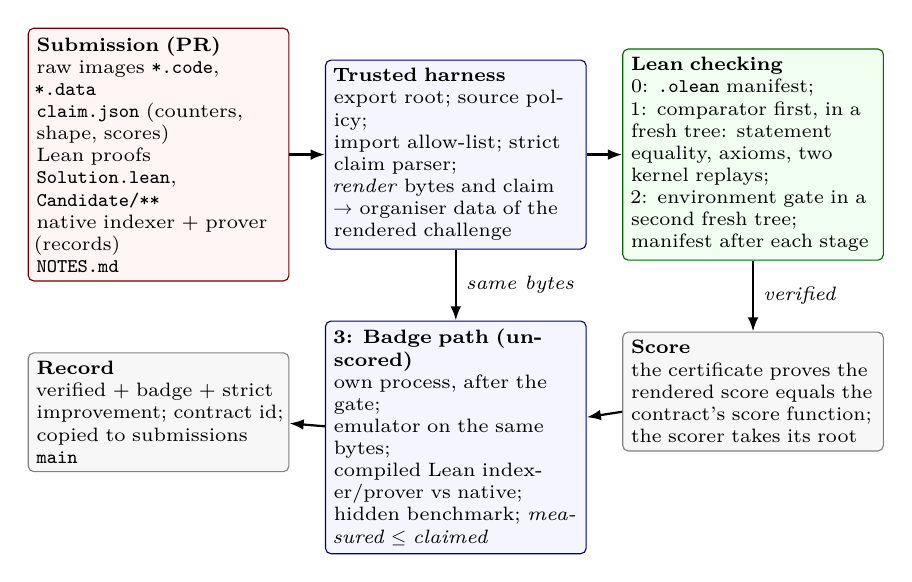
\begin{tikzpicture}[
  node distance=0.5cm and 0.45cm,
  box/.style={draw,rounded corners=2pt,align=left,font=\scriptsize,inner sep=3pt,text width=3.1cm},
  untr/.style={box,fill=red!4,draw=red!45!black},
  trus/.style={box,fill=blue!4,draw=blue!45!black},
  lean/.style={box,fill=green!6,draw=green!40!black},
  outb/.style={box,fill=black!3,draw=black!50},
  arr/.style={-{Latex[length=1.8mm]},thick},
  lab/.style={font=\scriptsize\itshape,align=center}]
\node[untr] (sub) {\textbf{Submission (PR)}\\
  raw images \code{*.code}, \code{*.data}\\
  \code{claim.json} (counters, shape, scores)\\
  Lean proofs \code{Solution.lean}, \code{Candidate/**}\\
  native indexer + prover (records)\\
  \code{NOTES.md}};
\node[trus, right=of sub] (har) {\textbf{Trusted harness}\\
  export root; source policy;\\
  import allow-list; strict claim parser;\\
  \emph{render} bytes and claim\\
  $\to$ organiser data of the\\ rendered challenge};
\node[lean, right=of har] (chk) {\textbf{Lean checking}\\
  0: \code{.olean} manifest;\\
  1: comparator first, in a\\ fresh tree: statement\\ equality, axioms, two\\ kernel replays;\\
  2: environment gate in a\\ second fresh tree;\\
  manifest after each stage};
\node[outb, below=0.9cm of chk] (score) {\textbf{Score}\\
  the certificate proves the\\
  rendered score equals the\\
  contract's score function;\\
  the scorer takes its root};
\node[trus, below=0.9cm of har] (badge) {\textbf{3: Badge path (unscored)}\\
  own process, after the gate;\\
  emulator on the same bytes;\\
  compiled Lean indexer/prover vs native;\\
  hidden benchmark; \emph{measured} $\le$ \emph{claimed}};
\node[outb, below=0.9cm of sub] (rec) {\textbf{Record}\\
  verified + badge + strict\\
  improvement; contract id;\\
  copied to submissions \code{main}};
\draw[arr] (sub) -- (har);
\draw[arr] (har) -- (chk);
\draw[arr] (chk) -- node[lab,right]{verified} (score);
\draw[arr] (har) -- node[lab,right]{same bytes} (badge);
\draw[arr] (score) -- (badge);
\draw[arr] (badge) -- (rec);
\end{tikzpicture}
\caption{The recursion.fast pipeline. Red: untrusted inputs. Blue: trusted software. Green: Lean
kernel checking. Stages run in the order of Decision~A-3. The proved score never depends on running
candidate code; the badge path runs candidate binaries in a sandbox and gates only record
eligibility. The v0.3 harness implements stages 0--2 and a hook for stage 3; the badge checks and
the emulator are specified but not yet built (\cref{sec:architecture}).}
\label{fig:obj-pipeline}
\end{figure}

\subsection{What is optimized, and why}\label{subsec:obj-what}

\paragraph{Primary objective: the cost of one recursion step.} The brief's \enquote{as efficient as
possible} admits four readings (\cref{sec:brief-review}): the cost of the final verifier, the cost
of one recursion step, proof size, and prover time. recursion.fast optimizes the second. In a
recursive proof system the inner verifier is executed inside a proof at every node of the
recursion tree, so its cost dominates the total prover work, while the final verifier runs once.
The recursion-step cost also subsumes the final-verifier cost, since a decider is itself a
verifier program. Proof size and prover time pull against verifier cost (a lower code rate shrinks
proofs and verifier work and inflates the prover); they enter as constraints and secondary
displays (\cref{sec:cost}), not as an arbitrary exchange rate inside the primary score.

\paragraph{Operationalization.} \enquote{Cost} means a \emph{vector} of instruction counts on one
fixed, contract-owned machine: RV64IM with all W-forms plus the Zbc carry-less multiplications,
with an oracle-query system call that stands for a Merkle opening (\cref{sec:protocol}). The vector
has 18 counters: instructions by class, first-touched memory words and pages, and query counts,
Merkle levels and leaf bytes. A submission proves, in Lean, an upper bound $c_k$ on this vector for
\emph{every accepting run} of its verifier image at each of three size classes
$k\in\{16,20,24\}$ (constraint systems with up to $2^k$ rows and columns). The score weights $c_k$
under four calibrated zkVM cost profiles, adds a static Fiat--Shamir surcharge and a proof-byte
charge, applies a soft penalty on prover-oracle blow-up, and takes the geometric mean over profiles
and classes (\cref{sec:cost}). The score function is a Lean definition of the contract, and the
certificate proves that the claimed score is its value. The score is therefore a theorem about the
exact bytes the deployed verifier would execute, not a measurement. A secondary latency board
scores a deterministic pipeline timing model with fork-join harts (\cref{subsec:cost-lat}).

\paragraph{Why accepting runs.} In recursion the circuit proves \enquote{the verifier accepted
$\pi$}; only accepting executions are ever arithmetized, and a zkVM's trace length is the executed
instruction count. A rejecting run is never proved. The maximum over accepting runs is thus
exactly the quantity a recursion step pays, and a maximum over \emph{all} runs over-approximates it
by the most expensive rejecting path, which no deployment pays except under attack. The bound is
not an average and not a measurement on honest proofs: by perfect completeness it covers every
honest run at every challenge vector, and it also covers every accepting run on an adversarial
transcript, including accepting runs on false statements. A verifier cannot make acceptance cheap
on true statements and expensive on false ones, because it cannot tell them apart; any
\enquote{fast accept} path must itself be sound, and then it is simply a cheaper verifier. Rejecting
runs are bounded by the contract's fuel constant ($2^{36}$ steps per hart), and fuel exhaustion is a
rejection (\cref{subsec:proto-machine}). The price is that the deployed decider's denial-of-service
exposure is bounded only by the fuel: $2^{36}$ steps for an image without harts, and
$(\#\mathrm{spawns}+1)\cdot2^{36}$ with harts, since a child runs on its parent's remaining fuel. An
optional all-runs badge is planned; it is not part of contract v0.3.

\paragraph{Relation to the brief's ambitious variant.} The brief's end state arithmetizes the
verifier and measures a 2-to-1 recursion step. We schedule this as a later score track (T3): wall
time is not reproducible, the RISC-V-to-constraint arithmetizer would be a large trusted artifact,
and the best modelled verifiers (\cref{subsec:bench-trajectory}) are 9--29 times too large for a
self-recursion fixed point inside the $2^{24}$ class (\cref{subsec:rec-t3}). The v1 proxy, the
instruction count of the fold verifier on the contract machine, is exactly what a fixed zkVM would
arithmetize.

\subsection{What counts as an interesting verifier architecture}\label{subsec:obj-interesting}

The competition succeeds if the leaderboard is populated by verifier \emph{architectures}, not by
assembly micro-optimizations of one known design, and not by artifacts of the rules. We call a
submission architecturally interesting if it is
\begin{enumerate}[nosep]
\item \emph{general}: one verifier image for every rank-1 constraint system (R1CS) of the class,
  with the circuit entering only through a short verification key and a committed index oracle
  (holography; \cref{subsec:bg-r1cs});
\item \emph{succinct}: its accepting-run cost is sublinear in the number of nonzero matrix entries,
  which in practice means a polynomial IOP combined with a hash-based polynomial commitment or
  proximity test;
\item \emph{provably sound at the stated level}: round-by-round errors of at most $2^{-128}$ per
  round, proved in Lean in the proven proximity regimes, or in a separate, labelled track under a
  published and named hypothesis (\cref{subsec:sec-hypotheses});
\item \emph{recursion-shaped}: it either verifies a full proof or, in the accumulation track (T2),
  folds two accumulators into one of fixed size and defers work to a decider (\cref{sec:recursion}).
\end{enumerate}
The intended design space is wide: sumcheck-based interactive oracle proofs such as Spartan
\cite{Set20-Spartan} and GKR-style memory checking for the sparse index; Reed--Solomon IOPPs over
binary additive domains such as WHIR \cite{ACFY24-WHIR}, BaseFold \cite{ZCF24-BaseFold},
FRI-Binius \cite{DP24-FRIBinius} and Ligerito \cite{NA25-Ligerito}; tensor-code commitments in the
Ligero/Brakedown line \cite{AHIV17-Ligero,GLSTW23-Brakedown}; holographic compilers in the
Marlin/COS line \cite{CHMMVW20-Marlin,COS20}; and hash-based accumulation such as WARP
\cite{BCFW25-WARP}, Arc \cite{BMNW25-Arc} and Blaze \cite{BCFRRZ25-Blaze}. The cost model is
calibrated so that the main levers are protocol choices. In a modelled Spartan-plus-binary-WHIR
verifier at $2^{24}$, the openings of the index commitment and of the witness commitment take
93\% of the cost; that cost is set by the proven query count, the leaf size and folding schedule,
and the size of the index commitment. Hand-tuning the extension-field kernels moves the total by
about 15\% (\cref{sec:cost}).

Equally explicit is what the rules must \emph{not} reward: special-casing the benchmark circuit or
its instances; lookup tables in an unbounded image or verification key; free computation by the
trusted harness (for example, powers of a challenge precomputed on the input tape); typed prover
messages that silently promise a property, such as low degree, that the deployed verifier never
checks; and protocols whose per-round error is small only because the number of rounds is
unbounded. Each of these is a concrete attack found during design review, and each is closed by a
rule cited where it is introduced.

\subsection{Design principles}\label{subsec:obj-principles}

\begin{description}[leftmargin=0pt,itemsep=2pt]
\item[P1. A small, auditable trusted base.] Everything a reader must accept is listed in one table
  (\cref{tab:arch-trusted}). The trusted Lean contract is 796 code lines (v0.3; v0.2 had 582) over
  Lean core, Mathlib and a vendored RISC-V model (listings in \cref{sec:appendix-contract}),
  and imports neither ArkLib nor CompPoly; bridges to those libraries are kernel-checked but
  untrusted. The growth from v0.2 is the cost model and the latency board: counters, timer, harts,
  profiles and score functions. The security definitions are statements about finite sets
  (\enquote{at most an $\eps$-fraction of challenges is bad}) with an existentially quantified
  state function, and no probability monad in the audited text.
\item[P2. A large design space.] The contract fixes the relation, the fields, the machine and the
  shapes of messages and challenges, and nothing about the protocol. Any public-coin holographic
  interactive oracle proof expressible with raw field-vector messages and contract-typed challenges
  is admissible. Organizers ship an untrusted, kernel-checked library (machine facts, a symbolic
  executor, verified field routines, IOP components, eventually a commitment scheme) so that the
  proof burden does not select designs.
\item[P3. Scores are proved, not measured.] The score is a Lean function of scalars that appear
  in kernel-checked theorem statements, and its value is itself a certificate clause. Measurements on hidden benchmarks are unscored
  demonstrations, a differential test of the trusted machine semantics, and a gate on record
  eligibility (\cref{subsec:arch-badge}).
\item[P4. A class-uniform cost theorem.] Knowledge soundness does not forbid
  hard-coding (the extractor is existential and may carry a benchmark witness). Overfitting is
  therefore excluded by the \emph{cost} statement, which quantifies over every index of a class
  shape, every public input, every prover message and every challenge, so that a fast path for one
  circuit cannot lower the score (\cref{subsec:bench-hardcode}).
\item[P5. Honest labelling.] Every record states precisely what is proved. With Lean extractors
  of unbounded running time, the base-level knowledge certificate is equivalent to round-by-round
  \emph{soundness}, and records say so (\cref{subsec:sec-extractor}); records under a named
  hypothesis are flagged with its version; one-step accumulation results are labelled one-step until
  the tree theorem exists; the gap from the interactive model to the deployed hash-based argument is
  stated as cited theorems and named deployment assumptions, never as Lean hypotheses.
\end{description}

\subsection{Non-goals}\label{subsec:obj-nongoals}

\begin{description}[leftmargin=0pt,itemsep=2pt]
\item[Zero knowledge.] Recursion needs succinctness and knowledge soundness, not privacy; zero
  knowledge would add a second simulation-based definition to the trusted text and is out of scope
  in v1.
\item[Quantum adversaries.] The statements proved in Lean are information-theoretic: they hold
  against unbounded adversaries. The compilation to a hash-based argument is cited in
  the classical random-oracle model only; a quantum random-oracle analysis \cite{CMS19} has worse
  constants and is not claimed.
\item[A prover-time score in v1.] The honest prover is a Lean specification proved complete; its
  running time is not observable from a Lean term. Prover cost is constrained statically
  (oracle-length caps and a soft blow-up factor in the score) and practically (a native prover must
  produce accepting proofs within a wall-clock and memory budget before a record is granted). A
  proved prover-cost bound would require a RISC-V prover with a refinement proof, which is far beyond
  any check budget (\cref{sec:cost}).
\item[Arithmetized recursion in v1.] Proving \enquote{the verifier accepted} inside the next proof
  needs a trusted RISC-V-to-constraint compiler and, for hash-compiled verifiers, a recursion
  heuristic that no random-oracle theorem justifies \cite{BCG24-RelROM}. v1 scores the fold
  verifier's cost on the machine; full recursion is a target schema (security level L4, score track
  T3; \cref{sec:recursion}).
\end{description}

% Provenance: copied from the design workspace CambridgePQ/recursion.fast, `report/sections/03-background.tex`, on 2026-10-19. Read-only copy; the source is authoritative.
% 03-background -- written by W1 (background for cryptographers and formal-methods readers)
% Unicode in listings: listings reorders non-ASCII glyphs under LuaLaTeX unless they are
% declared as literates (they would otherwise be emitted out of order, e.g. after a parenthesis).
\section{Background}\label{sec:background}

This section fixes notation and records the state of the art on which the competition design
rests. It has two audiences. Cryptographers should find
\cref{subsec:bg-lean} (what a Lean proof does and does not certify) self-contained. Formal-methods
readers should find the same for \cref{subsec:bg-r1cs,subsec:bg-iop,subsec:bg-bcs,subsec:bg-proximity,subsec:bg-binary,subsec:bg-costs,subsec:bg-recursion}.
Claims marked \emph{(unverified)} could not be confirmed from a primary source; repository facts
are cited as \repo{repo@commit} with a path, from the research notes behind this report.

Throughout, $\F$ is a finite field, $\lambda$ is a security parameter in bits, and
$[n]=\{1,\dots,n\}$. A probability bound is \emph{concrete} if it is stated as a function of the
parameters, without asymptotic notation. All adversaries in information-theoretic statements are
computationally unbounded.

%-----------------------------------------------------------------------------------------------
\subsection{R1CS, indexed relations and holography}\label{subsec:bg-r1cs}

\begin{definition}[R1CS]\label{def:bg-r1cs}
Fix sizes $m$ (constraints), $n_x$ (public inputs) and $n_w$ (witness variables), and let
$N = 1+n_x+n_w$. An \emph{R1CS index} is a triple $i=(A,B,C)$ of matrices in $\F^{m\times N}$.
An \emph{instance} is $x\in\F^{n_x}$ and a \emph{witness} is $w\in\F^{n_w}$. With
$z=(1,x,w)\in\F^N$,
\[
  (i,x,w)\in\Rrcs \iff (A z)\circ(B z) = C z ,
\]
where $\circ$ is the entrywise (Hadamard) product. The \emph{sparsity} is
$\mathsf{nnz}(i) = |\mathrm{supp}\,A|+|\mathrm{supp}\,B|+|\mathrm{supp}\,C|$, the number of nonzero
entries (some papers use the maximum of the three counts instead; the two differ by a factor of at
most $3$).
\end{definition}

The leading constant $1$ in $z$ lets affine constraints be written; ArkLib's
\lean{R1CS.relation} uses $z=(x,w)$ without it, so the competition restates the relation
locally.\footnote{\repo{ArkLib@db7005f}, \path{ArkLib/ProofSystem/ConstraintSystem/R1CS.lean:64}
(\lean{relation}); its field comments for $m$ and $n$ are also swapped (lines 32--33).}
recursion.fast instantiates $\F$ with the binary field $K=\mathrm{GF}(2^{64})$
(\cref{subsec:bg-binary}). R1CS is NP-complete, and a RISC-V execution trace, a hash chain or a SNARK verifier can all be
arithmetised into it; the matrices are then very sparse ($\mathsf{nnz}=O(m+N)$).

\paragraph{Indexed relations.} An \emph{indexed relation} $\R$ is a set of triples $(i,x,w)$:
the index $i$ is large and fixed in advance (here the matrices), the instance $x$ is small and
varies from proof to proof. Its language is $L(\R)=\{(i,x) : \exists w,\ (i,x,w)\in\R\}$
\cite{CHMMVW20-Marlin,COS20}, \cite[ch.~32]{CY24-Book}. Soundness for an indexed relation
quantifies over \emph{adversarially chosen} indices: the cheating prover outputs $(i,x)$ (and
auxiliary data) itself \cite[Def.~32.4.2]{CY24-Book}.

\paragraph{Why succinct verification of arbitrary R1CS needs preprocessing.} An arbitrary
(non-uniform) index has description length $\Theta(\mathsf{nnz}\cdot\log(mN|\F|))$ bits. A
verifier that receives $i$ as input therefore runs in time $\Omega(\mathsf{nnz})$ just to read it,
and checking $(Az)\circ(Bz)=Cz$ directly costs $\Theta(\mathsf{nnz})$ field operations. Succinct
verification is possible only if the cost of reading $i$ is paid once, by an \emph{indexer}.

\begin{definition}[Holographic proof system]\label{def:bg-holographic}
A holographic (preprocessing) proof system for $\R$ is a triple $(\Ind,\Prv,\Vrf)$. The
deterministic indexer computes, once per index, an encoding $\Ind(i)$ (the \emph{index oracle})
and a short verification key $\vk_i$. The prover receives $(i,x,w)$. The verifier receives
$(\vk_i,x)$ and \emph{oracle access} to $\Ind(i)$, and runs in time polylogarithmic in
$|i|$. In the compiled argument, $\vk_i$ contains a Merkle root of $\Ind(i)$, and the verifier's
queries to $\Ind(i)$ become authenticated openings \cite[ch.~32]{CY24-Book}.
\end{definition}

\paragraph{Spartan, Marlin, Fractal and COS.} \emph{Spartan} \cite{Set20-Spartan} reduces R1CS
satisfiability to a sumcheck over the multilinear extensions $\tilde A,\tilde B,\tilde C$ and
$\tilde z$. At the end the verifier needs $\tilde A(r_x,r_y)$, $\tilde B(r_x,r_y)$,
$\tilde C(r_x,r_y)$ at a random point. SPARK, Spartan's sparse-polynomial compiler, lets the
prover prove these evaluations against a commitment to the matrices computed in preprocessing
(Spartan's ``computation commitment''), so the verifier costs $O(\log^2 n)$ field operations plus
polynomial-commitment checks. \emph{Marlin} \cite{CHMMVW20-Marlin} introduced holographic
polynomial IOPs for R1CS, in which the indexer encodes each matrix by low-degree polynomials
(row, column, value) that the verifier queries. \emph{Fractal} \cite{COS20} gave holographic IOPs
with Reed--Solomon encodings and the COS transformation, the holographic analogue of BCS
(\cref{subsec:bg-bcs}). The result is transparent, plausibly post-quantum and recursive, and
\cite[ch.~32]{CY24-Book} formalises it. Pairing Spartan's information-theoretic core with a
hash-based polynomial commitment (WHIR or BaseFold, \cref{subsec:bg-costs}) yields a
hash-based R1CS verifier; STIR estimates about $220$\,KiB for an $n=2^{24}$ R1CS at $128$ bits and
$\rho=1/2$ \cite{ACFY24-STIR}.

%-----------------------------------------------------------------------------------------------
\subsection{Interactive oracle proofs and round-by-round knowledge soundness}\label{subsec:bg-iop}

\paragraph{IOPs.} An \emph{interactive oracle proof} (IOP)
\cite{BCS16,RRR16} with $k$ rounds runs as follows. In round $j\in[k]$ the prover sends an
\emph{oracle} $\Pi_j\in\Sigma_j^{\ell_j}$, a string the verifier may later read at chosen
positions. The verifier then replies with a challenge $\rho_j$. After the last round the
verifier queries the oracles (and $\Ind(i)$, if holographic) and accepts or rejects. The IOP is
\emph{public-coin} if every $\rho_j$ is uniform on a finite set $C_j$ and independent of
everything else, so that the verifier's randomness is its messages; only public-coin IOPs can be
compiled by Fiat--Shamir. We write $\mathrm{tr}_{<j}$ for the partial transcript before round $j$,
$\ell=\sum_j\ell_j$ for the total oracle length, and $q$ for the number of queries. An \emph{IOP of
proximity} (IOPP) instead gives the verifier oracle access to its input $f$ and asks it to reject
when $f$ is $\delta$-far from a code (\cref{subsec:bg-proximity}). FRI, STIR and WHIR are IOPPs.

Fix an indexed relation $\R$ and a public-coin holographic IOP $(\Ind,\Prv,\Vrf)$. Write
$\langle \tilde\Prv,\Vrf\rangle(i,x)\in\{0,1\}$ for the verifier's decision when it interacts
with a (possibly malicious) prover $\tilde\Prv$, the probability being over the challenges.

\begin{definition}[Completeness, soundness, knowledge soundness]\label{def:bg-ks}
The IOP has
\begin{itemize}[nosep]
  \item \emph{perfect completeness} if $\Pr[\langle\Prv(i,x,w),\Vrf\rangle(i,x)=1]=1$ for every
    $(i,x,w)\in\R$;
  \item \emph{soundness error} $\eps$ if $\Pr[\langle\tilde\Prv,\Vrf\rangle(i,x)=1]\le\eps$ for
    every $(i,x)\notin L(\R)$ and every $\tilde\Prv$;
  \item \emph{(straight-line) knowledge error} $\kappa$ if there is an extractor $\Ext$ such that for
    every $(i,x)$ and every $\tilde\Prv$,
    \[ \Pr\bigl[\langle\tilde\Prv,\Vrf\rangle(i,x)=1 \ \wedge\ (i,x,\Ext(i,x,\Pi_1,\dots,\Pi_k))\notin\R\bigr]\le\kappa, \]
    where $\Ext$ sees the prover's oracles but not its code (it is \emph{straight-line}, i.e.\ it
    does not rewind). Cryptographic definitions require $\Ext$ to run in polynomial time.
\end{itemize}
\end{definition}

Completeness is not a formality in an adversarial competition: a verifier that rejects
everything is trivially sound, and only completeness excludes it.

\paragraph{Round-by-round soundness.} Soundness bounds the total probability of acceptance;
Fiat--Shamir needs a stronger, per-round property. Round-by-round (RBR) soundness, introduced by
Canetti et al.\ \cite{CCHLRRW19}, requires that a false statement stay ``doomed'' after each
round except with small probability over that round's challenge.

\begin{definition}[State function; RBR soundness {\cite{CCHLRRW19}, \cite[Defs.~31.1.1--31.1.2]{CY24-Book}}]\label{def:bg-rbr}
A \emph{state function} is a deterministic (possibly inefficient) predicate
$\mathsf{St}((i,x),\mathrm{tr})\in\{0,1\}$ on partial transcripts such that, for $(i,x)\notin L(\R)$:
(i) $\mathsf{St}((i,x),\emptyset)=0$; (ii) prover moves cannot leave the doomed state:
$\mathsf{St}(\mathrm{tr})=0\Rightarrow\mathsf{St}(\mathrm{tr}\|\Pi)=0$ for every $\Pi$; and
(iii) if $\mathsf{St}(\mathrm{tr})=0$ on a full transcript then $\Vrf$ rejects. The IOP has
\emph{RBR soundness error} $(\eps_1,\dots,\eps_k)$ if some state function satisfies, for every
$(i,x)\notin L(\R)$, every $j$ and every prefix $\mathrm{tr}\|\Pi_j$ with
$\mathsf{St}(\mathrm{tr}\|\Pi_j)=0$,
\[ \Pr_{\rho_j\leftarrow C_j}\bigl[\mathsf{St}(\mathrm{tr}\|\Pi_j\|\rho_j)=1\bigr]\le\eps_j . \]
\end{definition}

Only verifier randomness can flip a state from $0$ to $1$, so a union bound gives soundness error
at most $\sum_j\eps_j\le k\cdot\max_j\eps_j$ \cite[Claim~31.1.3]{CY24-Book}.

\paragraph{RBR knowledge soundness: three variants.} The knowledge analogue
\cite{CMS19,COS20} comes in (at least) three variants that differ in what the extractor sees:
CMS19's, whose extractor sees the transcript prefix \cite[Def.~8.5]{CMS19}; the book's, whose
single extractor sees all prover strings of the continued execution \cite[Def.~31.1.6]{CY24-Book}
(\cref{def:bg-rbrks-cy}); and WARP's per-round backward extractor \cite[Defs.~4.1--4.2]{BCFW25-WARP}
(\cref{def:bg-rbrks-warp}). The competition must pin exactly one of them (\cref{sec:security}).

\begin{definition}[RBR-KS, global extractor; paraphrasing {\cite[Def.~31.1.6]{CY24-Book}}]\label{def:bg-rbrks-cy}
There are a state function $\mathsf{St}$ and a polynomial-time extractor $\Ext$ that sees only
prover strings (hence is straight-line) such that for every $(i,x)$, every malicious prover
$\tilde\Prv$, every $j$ and every prefix with $\mathsf{St}(\mathrm{tr}\|\Pi_j)=0$,
\[ \Pr_{\rho_j,\ \tilde\Prv}\bigl[\mathsf{St}(\mathrm{tr}\|\Pi_j\|\rho_j)=1 \ \wedge\
   (i,x,\Ext(i,x,\vec\Pi))\notin\R\bigr]\le\kappa_j , \]
where the probability is over $\rho_j$ and the continuation $(\Pi_{j+1},\dots,\Pi_k)$ produced by
$\tilde\Prv$, and $\vec\Pi$ is the list of \emph{all} prover oracles of that execution, including
those sent after round $j$.
\end{definition}

The second variant replaces the single extractor by a chain of per-round maps that pull a witness
backwards through the transcript. It is due to WARP \cite[Defs.~4.1--4.2, informally
2.6--2.7]{BCFW25-WARP} and is the
form ArkLib implements (\lean{KnowledgeStateFunction} with \lean{Extractor.RoundByRound}).
Position the $n=2k$ messages in order (prover message, then challenge) and index stages by
$m\in\{0,\dots,n\}$.

\begin{definition}[RBR-KS, per-round backward extractor {\cite[Def.~4.2, informally Def.~2.7]{BCFW25-WARP}}]\label{def:bg-rbrks-warp}
A \emph{knowledge state function} is a family of predicates $S_m(s,\mathrm{tr},w)$ on statements
$s=(i,x)$, stage-$m$ transcripts and intermediate witnesses $w\in W_m$ (with $W_0$ the witness
type of $\R$). It comes with extractor maps $E_m:\ (s,\mathrm{tr}\|a,w)\mapsto w'$ from $W_{m+1}$
to $W_m$ and $E_{\mathrm{out}}$ into $W_n$, satisfying three laws:
\begin{itemize}[nosep]
  \item (empty) $S_0(s,\emptyset,w)\iff (s,w)\in\R$;
  \item (prover moves) if message $m$ is the prover's, then
    $S_{m+1}(s,\mathrm{tr}\|\Pi,w)\Rightarrow S_m(s,\mathrm{tr},E_m(s,\mathrm{tr}\|\Pi,w))$;
  \item (full) if $\Vrf(s,\mathrm{tr})=\mathsf{some}\ s'$ and $(s',w')\in\R_{\mathrm{out}}$, then
    $S_n(s,\mathrm{tr},E_{\mathrm{out}}(s,\mathrm{tr},w'))$; for a proof system,
    $\R_{\mathrm{out}}$ is trivial (\cref{def:bg-rok}).
\end{itemize}
For a challenge position $m$ and prefix $\mathrm{tr}$, a challenge $c\in C_m$ is \emph{bad} if
$\exists w:\ \neg S_m(s,\mathrm{tr},E_m(s,\mathrm{tr}\|c,w))\wedge S_{m+1}(s,\mathrm{tr}\|c,w)$.
The verifier is \emph{(worst-case) RBR knowledge sound} with errors $(\eps_m)$ if, for every $s$,
every challenge position $m$ and every prefix $\mathrm{tr}$,
\[ \#\{c\in C_m : c \text{ bad}\}\ \le\ \eps_m\cdot|C_m| . \]
\end{definition}

\begin{remark}[How the variants differ]\label[remark]{rem:bg-variants}
(1) \emph{Extractor shape.} \Cref{def:bg-rbrks-cy} has one extractor that sees every prover
string. \Cref{def:bg-rbrks-warp} has one local map per round, and extraction only needs to
\emph{fail} at a challenge. WARP shows that its notion is implied by the CMS19-style notion
(adapted to reductions) \cite[App.~C]{BCFW25-WARP} and states that the relaxation is strict, which
is what admits codes not known to have an efficient \emph{error-tolerant} decoder; it does not
compare its notion with the book's. ArkLib further
generalises the definition in two documented ways: the maps may transform the witness across
prover moves, and the full-transcript law is one-directional.\footnote{\repo{ArkLib@db7005f},
\path{ArkLib/OracleReduction/Security/RoundByRound.lean:155-164} (docstring: deviations from
ABF26 Def.~A.5, in ArkLib's numbering).} (2) \emph{Worst case versus average.} \Cref{def:bg-rbrks-warp} quantifies over
every prefix, which matches the literature. ArkLib's default \lean{rbrKnowledgeSoundness} instead
lets the prover sample the prefix and bounds the mixture, which is weaker; the worst-case form
\lean{rbrKnowledgeSoundnessWorstCase} exists, and the implication worst-case $\Rightarrow$
averaged is proved.\footnote{\repo{ArkLib@db7005f},
\path{ArkLib/OracleReduction/Security/RoundByRound.lean:539} (definition) and \texttt{:609}
(implication).} (3) \emph{Efficiency.} Cryptographic definitions require a polynomial-time
extractor; ArkLib's extractor maps are arbitrary Lean functions (\cref{subsec:bg-lean}).
\end{remark}

\paragraph{State-restoration soundness.} The property that Fiat--Shamir and BCS actually consume
is \emph{state-restoration} (SR) soundness \cite{BCS16}, \cite[Defs.~23.2.2--23.2.3]{CY24-Book}.
In the SR game the malicious prover talks to a verifier that it may \emph{rewind}: at each of at
most $t$ moves it picks any previously reached verifier state (a partial transcript), appends a
prover message, and receives a fresh challenge. It wins if some complete transcript in the
resulting tree is accepting while $(i,x)\notin L(\R)$ (soundness, error $\eps^{\mathrm{sr}}(t)$),
or is accepting while the extractor, given the tree, fails to output a witness (knowledge, error
$\kappa^{\mathrm{sr}}(t)$). This models a Fiat--Shamir prover, which can recompute a hash on any
modified prefix.

\begin{theorem}[Relations between the notions]\label[theorem]{thm:bg-rbr-sr}
Let $\eps_{\mathrm{rbr}}=\max_j\eps_j$ and $\kappa_{\mathrm{rbr}}=\max_j\kappa_j$.
\begin{enumerate}[nosep]
  \item RBR-KS with errors $(\kappa_j)$ implies RBR soundness with the same errors.
  \item RBR soundness implies soundness error $\sum_j\eps_j$, and RBR-KS implies straight-line
    knowledge error $\sum_j\kappa_j$ \cite[Claim~31.1.3]{CY24-Book}.
  \item $\eps^{\mathrm{sr}}(t)\le(t+k)\cdot\eps_{\mathrm{rbr}}$ \cite[Thm.~31.2.1]{CY24-Book}, and
    $\kappa^{\mathrm{sr}}(t)\le(t+k)\cdot\kappa_{\mathrm{rbr}}$ with a straight-line SR extractor
    for the book's notion \cite[Thm.~31.3.1]{CY24-Book}. For the backward-extractor variant, the
    same $(t+k)\cdot\kappa_{\mathrm{rbr}}$ bound is \cite[Thm.~2.8, formally Thm.~B.4 with
    Constr.~B.5]{BCFW25-WARP}, with extraction time $\sum_i\mathit{et}_i$.
  \item For interactive proofs, RBR soundness and SR soundness are qualitatively (asymptotically) equivalent, and
    neither follows from Fiat--Shamir soundness in the random-oracle model \cite{Hol19}.
\end{enumerate}
\end{theorem}

Item~1 is proved in ArkLib.\footnote{\repo{ArkLib@db7005f},
\path{ArkLib/OracleReduction/Security/Implications.lean:87}.} The implications to plain
soundness and knowledge soundness in item~2, and all SR implications in ArkLib's legacy layer, are
currently \lean{sorry}. ArkLib's newer native \lean{Interaction} layer proves an SR knowledge bound
$(Q+\#\text{rounds})\cdot\eps$, sorry-free, for a fixed-round presentation with finite message and
challenge types. It is not yet connected to the legacy definitions
(\cref{subsec:bg-lean}).\footnote{\repo{ArkLib@db7005f},
\path{ArkLib/Interaction/Oracle/Security/StateRestorationGame.lean:102}
(\lean{stateRestoration\_knowledge\_soundness}).}

The alternative route to Fiat--Shamir security is \emph{special soundness}. For multi-round
special-sound protocols, Attema, Fehr and Klo\ss{} show that the Fiat--Shamir knowledge error
grows only linearly in the number of random-oracle queries \cite{AFK22}. Block et al.\ relate the
generalised notions for IOPs: generalised special soundness implies generalised RBR soundness,
and generalised RBR-KS implies generalised special soundness, but not conversely
\cite{BGTZ23}. For hash-based IOPs, RBR (knowledge) soundness is the notion that has actually been
proven: for FRI's Fiat--Shamir security \cite{BGKTTZ23-FSFRI}, for STIR (RBR soundness)
\cite{ACFY24-STIR} and for WHIR (RBR-KS) \cite{ACFY24-WHIR}.

%-----------------------------------------------------------------------------------------------
\subsection{From IOPs to SNARKs: BCS and Fiat--Shamir}\label{subsec:bg-bcs}

\paragraph{The BCS transformation.} Ben-Sasson, Chiesa and Spooner \cite{BCS16} compile a
public-coin IOP into a non-interactive argument in the random-oracle model (ROM) as follows. The
prover commits to each oracle $\Pi_j$ with a Merkle tree, whose leaves and nodes are hashed with
the random oracle $H$. It derives $\rho_j$ by hashing the previous state and the new root
$\mathrm{rt}_j$ (with a salt). It derives the query positions from the final state, and it sends
the queried symbols with their authentication paths. The verifier recomputes every challenge and
checks every path. Let $t$ be the adversary's query budget to $H$, $\lambda$ the output length of
$H$ in bits, $k$ the round count and $\ell$ the total oracle length.

\begin{theorem}[BCS, concrete bounds {\cite[Thms.~25.2.1 and 26.1.1 (straight-line clause)]{CY24-Book}}]\label[theorem]{thm:bg-bcs}
For $t\ge 2(\log\ell+1)\cdot\ell$, with $\ell=\sum_j\ell_j$ (the book's condition under which the
Merkle and collision terms combine), the BCS argument has soundness and straight-line knowledge errors
\[
  \eps_{\mathrm{BCS}}(t)\le (t+k)\cdot\eps_{\mathrm{rbr}} + \frac{3.5\,t^2}{2^{\lambda}},\qquad
  \kappa_{\mathrm{BCS}}(t)\le (t+k)\cdot\kappa_{\mathrm{rbr}} + \frac{3.5\,t^2}{2^{\lambda}} .
\]
The extractor runs in time $\mathit{et}^{\mathrm{sr}}+\mathit{et}^{\mathrm{mm}}_{\mathrm{MT}}
+O(r_{\max}\cdot k\cdot t\log t)$: the SR extractor's time, the Merkle extractor's time, and a
term with $r_{\max}=\max_j\log|C_j|$ the largest challenge length. (The book's main knowledge
statements are for rewinding extractors; straight-line extraction is their \enquote{moreover}
clause.) For the holographic COS variant, which commits to $\Ind(i)$ once and places the root in
$\vk_i$, the bound gains a term $4\ell_0^2/2^\lambda$ for an index oracle of length $\ell_0$; with
$\ell:=\ell_0+\sum_j\ell_j$ and $t\ge2\ell_0$ it is $(t+k)\cdot\eps_{\mathrm{rbr}}+4.5\,t^2/2^\lambda$
(soundness \cite[Thm.~32.8.9]{CY24-Book}; knowledge, straight-line clause, \cite[Thm.~32.8.10]{CY24-Book}).
\end{theorem}

\paragraph{Reading the bound.} The factor $(t+k)$ is the price of state restoration. A Lean bound
of $2^{-\lambda_r}$ per round therefore yields only about $2^{-(\lambda_r-\tau)}$ against an
adversary making $t=2^\tau$ hash queries. For example, with
$\eps_{\mathrm{rbr}}\le 2^{-128}$, $\lambda=256$ and $2k\le t\le 2^{124}$ (with $t$ replaced by
$\max(t,t^*)$ in the hash term below the side condition's threshold $t^*$, \cref{subsec:sec-cap}),
we get $\kappa(t)\le 1.5\,t/2^{128}+4.5\,t^2/2^{256}\le t/2^{127}$, which is sig.golf's $Q/2^{127}$
convention (\cref{sec:prior}). With $k\le t$ alone, the first term already equals $t/2^{127}$ and
the bound exceeds it by the (negligible) collision term. Grinding (proof-of-work) adds bits to
individual rounds \cite{ethSTARK21}. Deployed systems implement
Fiat--Shamir with a duplex sponge rather than independent random oracles; Chiesa and Orr\`u
analyse that setting in the ideal-permutation model \cite{CO25-DuplexFS}.

\begin{figure}[t]
\centering
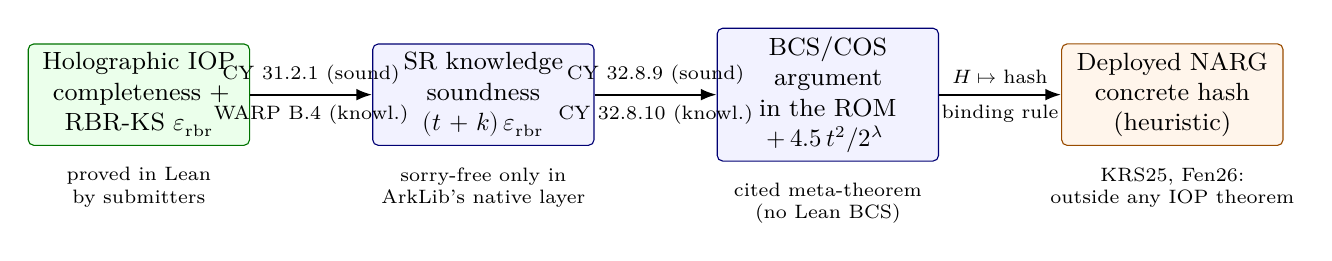
\begin{tikzpicture}[
  box/.style={draw,rounded corners=2pt,align=center,font=\small,minimum height=1.25cm,text width=2.6cm,inner sep=3pt},
  lean/.style={box,fill=green!8,draw=green!45!black},
  cited/.style={box,fill=blue!5,draw=blue!45!black},
  heur/.style={box,fill=orange!8,draw=orange!60!black},
  arr/.style={-{Latex[length=2mm]},thick},
  lab/.style={font=\scriptsize,align=center}]
\node[lean]  (iop) {Holographic IOP\\ completeness +\\ RBR-KS $\eps_{\mathrm{rbr}}$};
\node[cited, right=1.55cm of iop] (sr) {SR knowledge\\ soundness\\ $(t+k)\,\eps_{\mathrm{rbr}}$};
\node[cited, right=1.55cm of sr] (bcs) {BCS/COS argument\\ in the ROM\\ $+\,4.5\,t^2/2^{\lambda}$};
\node[heur, right=1.55cm of bcs] (fs) {Deployed NARG\\ concrete hash\\ (heuristic)};
\draw[arr] (iop) -- node[lab,above]{CY 31.2.1 (sound)}node[lab,below]{WARP B.4 (knowl.)} (sr);
\draw[arr] (sr) -- node[lab,above]{CY 32.8.9 (sound)}node[lab,below]{CY 32.8.10 (knowl.)} (bcs);
\draw[arr] (bcs) -- node[lab,above]{$H\mapsto$ hash}node[lab,below]{binding rule} (fs);
\node[lab,below=0.15cm of iop] {proved in Lean\\ by submitters};
\node[lab,below=0.15cm of sr] {sorry-free only in\\ ArkLib's native layer};
\node[lab,below=0.15cm of bcs] {cited meta-theorem\\ (no Lean BCS)};
\node[lab,below=0.15cm of fs] {KRS25, Fen26:\\ outside any IOP theorem};
\end{tikzpicture}
\caption{The security chain from an IOP to a deployed succinct argument, and which link is
machine-checked. Only the leftmost box is a Lean obligation in recursion.fast; the arrows are
theorems of the cited works; the last arrow is a heuristic that contract rules must protect.}
\label{fig:bg-pipeline}
\end{figure}

\paragraph{Fiat--Shamir pitfalls outside the IOP model.} Three classes of failure sit outside
\cref{thm:bg-bcs} because they concern how the oracle is instantiated or what is hashed.
\begin{enumerate}[nosep,label=(\roman*)]
\item \emph{Weak Fiat--Shamir.} Deriving challenges without hashing the statement lets a prover
  choose the statement after the challenges \cite{BPW12-WeakFS}. In the indexed setting the
  statement is $(i,x)$, so $\vk_i$ \emph{and} $x$ must be absorbed.
\item \emph{Hash inside the relation.} Khovratovich, Rothblum and Soukhanov give, for every
  concrete Fiat--Shamir hash, a circuit for which Fiat--Shamir-compiled GKR is not adaptively
  sound, even under the \emph{strong} transform that absorbs the statement (the circuit
  description). The circuit evaluates the hash on a transcript-predicting input \cite{KRS25}. Recursion
  meets this precondition by construction, because the proved circuit contains the verifier's
  hash.
\item \emph{Generated statements.} Fenzi extends this to R1CS instances \emph{generated by running
  an adversarial program}: when the conversion is expressive enough, the author of the program can
  break Fiat--Shamir soundness of any protocol in which an accepting transcript can be prepared
  before the statement is bound. Variants of Spartan and Aurora \cite{BCRSVW19-Aurora} are
  affected \cite{Fen26-GenR1CS}. The proven mitigation is to derive the first challenge from the
  \emph{generated statement}, meaning the R1CS (or its commitment) and the public input; soundness
  then reduces to that of the underlying protocol for the non-generated relation. (We read this
  paper only at the level of its abstract and the R7 summary.)
\end{enumerate}
In recursion.fast the R1CS is generated from programs, and the next layer's circuit contains the
hash. The design therefore makes the initial absorption a property of the trusted harness, not of
the submission: the transcript starts from
$H(\mathit{domSep}\,\|\,\mathit{contractId}\,\|\,\mathit{shapeHash}\,\|\,\mathit{claimHash}\,\|\,k\,\|\,\mathrm{MTroot}(\Ind(i))\,\|\,\vk_i\,\|\,x)$
(rule S-4 of \cref{subsec:sec-fs}). This answers (i) and (iii). It does not answer (ii), which
breaks the strong transform; that attack is part of the named deployment assumption of
\cref{subsec:rec-cannot}.

\paragraph{Sampler bias.} \Cref{thm:bg-bcs} treats challenges as uniform elements of $C_j$. An
implementation maps hash bits to field elements, and any fixed bad set gains at most the
statistical distance of that map from uniform, which therefore adds directly to each $\eps_j$.
Over a prime field, reducing a $b$-bit uniform integer modulo $p$ (write $2^b=Qp+r$, $0\le r<p$)
gives distance $r(p-r)/(p\,2^b)\le p/2^{b+2}$. For a 31-bit prime and $b=128$ this is about
$2^{-99}$, which would dominate a $2^{-128}$ round error, so implementations need rejection
sampling or $b\ge160$ bits per coordinate. Over $\mathrm{GF}(2^n)$ every $n$-bit string is an
element, so sampling is exactly uniform (\cref{subsec:bg-binary}).

\begin{takeaway}[What is and is not provable today]
The information-theoretic statement (completeness and RBR-KS of a holographic IOP) is the only
link that submissions can prove in Lean with current libraries. ArkLib has no BCS transform and
no Fiat--Shamir soundness theorem in its legacy layer; its Fiat--Shamir completeness lemma is
\lean{sorry}. The compiled bound is therefore a cited meta-theorem with the explicit form
$(t+k)\,\eps_{\mathrm{rbr}}+4.5\,\max(t,t^*)^2/2^\lambda$, with $t^*$ the side condition's threshold
(\cref{subsec:sec-cap}). Weak-FS and generated-statement attacks are excluded by contract rules,
not by theorems; the hash-in-circuit attack is excluded by neither and is a named deployment
assumption.
\end{takeaway}

%-----------------------------------------------------------------------------------------------
\subsection{Proximity gaps: what is proven and what has been refuted}\label{subsec:bg-proximity}

Let $C=\mathrm{RS}[\F,D,k]$ be the Reed--Solomon code of evaluations on $D\subseteq\F$, $|D|=n$, of
polynomials of degree $<k$. Its rate is $\rho=k/n$ and its relative distance is
$\delta_C=1-\rho+1/n$. Write $\Delta(u,C)$ for the relative Hamming distance from $u\in\F^D$ to
$C$. Three radii matter: \emph{unique decoding} $\gamma<\delta_C/2\approx(1-\rho)/2$, where every
word has at most one codeword within $\gamma$; the \emph{Johnson radius} $1-\sqrt\rho$, up to which
lists are provably polynomial; and \emph{capacity} $1-\rho$.

\begin{definition}[Proximity gap; correlated agreement]\label{def:bg-ca}
The code $C$ has \emph{correlated agreement for lines} at radius $\gamma$ with exceptional count
$a$ if, for all $u_0,u_1\in\F^D$,
\begin{multline*}
  \bigl|\{z\in\F : \Delta(u_0+z\,u_1,\,C)\le\gamma\}\bigr|> a \\
  \Longrightarrow\ \exists S\subseteq D,\ |S|\ge(1-\gamma)n,\ \exists v_0,v_1\in C:\
  u_0|_S=v_0|_S,\ u_1|_S=v_1|_S.
\end{multline*}
The combination step of a batched or folded test then errs with probability about $a/|\F|$.
\emph{Mutual correlated agreement} (MCA), which WHIR needs \cite{ACFY24-WHIR}, additionally
requires the agreement set of the random combination itself to be one on which $u_0,u_1$ agree
with codewords, except with similar probability over $z$.
\end{definition}

The soundness error of FRI, STIR and WHIR decomposes into three terms. The batching or folding term
is proportional to $a/|\F|$ per round. The query term is about $(1-\gamma)^s$ for $s$ queries. The
third term comes from Fiat--Shamir (\cref{subsec:bg-bcs}). The radius $\gamma$ at which the gap
is \emph{proven} therefore sets the number of queries, and query count is the dominant verifier
cost.

\begin{table}[t]
\centering\small
\begin{tabularx}{\linewidth}{@{}l>{\raggedright\arraybackslash}Xl@{}}
\toprule
Regime & Result (exceptional count $a$; error $\approx a/|\F|$) & Status \\
\midrule
$\gamma<\delta_C/2$ (UD) & correlated agreement with $a\approx n$ \cite{BCIKS20} & proven \\
$\gamma\in(\delta_C/3,\delta_C/2-1/n)$ & $a=O(1)$ with arbitrarily small proximity loss \cite[Thm.~1.3]{BCHKS25} & proven \\
$\gamma<1-\sqrt\rho-\eta$ (JB) & $a=O(n^2/\eta^7)$ \cite{BCIKS20}; improved to $a=O(n/\eta^5)$ \cite[Thm.~1.5]{BCHKS25} & proven \\
MCA up to Johnson & for all polynomial generators (lines, powers, curves) \cite{BCGM25-MCA}; see also \cite{Hab25-MCA} & proven \\
past Johnson by $O(1)$ steps & MCA with relative gain $O(1/n)$ \cite{Jo26-MCA} & preprint \\
up to $1-\rho-\eta$ & optimal gaps for folded RS, multiplicity, subspace-design and \emph{random} RS codes \cite{GG25,GGSW26}; not smooth-domain RS & proven \\
\midrule
up to capacity, RS & BCIKS20 capacity conjecture: refuted for rate $\to0$, radius $\to1$ \cite{DG25-Dist} & refuted \\
up to capacity, RS & CA, WHIR MCA and DEEP-FRI list-decoding conjectures refuted in general form \cite{CS25-PGC} & refuted \\
at Johnson ($\eta=0$), char.~2, rate $\approx1/16$ & $n^{2-o(1)}$ exceptional points on random $\F_2$-subspaces \cite[Thm.~1.6, Cor.~1.7]{BCHKS25}; beyond-Johnson refuted for these codes & lower bound \\
DEEP-ALI, ethSTARK toy problem & attacks showing soundness is governed by list decodability \cite{BCHKS25} & refuted \\
near capacity, prime fields & lines with $2^{\Omega(1/\eta)}$ close points $z$ at $1-\rho-\eta$, $\eta=\Theta(1/\log n)$, on multiplicative subgroups \cite{KKH26}; $\ge n^{C}$ close points for primes $p\equiv1\bmod n$ at $\delta=(1-\rho)-\Omega(1/\log n)$ \cite{Kam26} & refuted \\
\bottomrule
\end{tabularx}
\caption{Proximity gaps for Reed--Solomon codes as of October 2026. ``Refuted'' means that
counterexamples exist in the stated regime, not that every restricted variant fails; open problems
are surveyed in \cite{ABF26}.}
\label{tab:bg-proximity}
\end{table}

Three consequences follow (\cref{tab:bg-proximity}). First, the ``up to capacity'' conjectures on
which most deployed parameter sets rest are false in at least some regimes. Crites and Stewart
propose a weakened ``list-decoding capacity'' conjecture, for prime $q$ up to the radius
$\delta$ with $H_q(\delta)\le1-\rho-\eta$, whose loss against capacity is at most
$1/\log_2q+1/n$ \cite{CS25-PGC}. Second, BCHKS25 show that improved proximity
gaps imply improved list decoding for all RS codes, so beyond-Johnson gaps first require
list-decoding progress \cite{BCHKS25}. Third, the capacity-achieving results of \cite{GG25,GGSW26}
cover codes that FRI-style protocols do not currently use, which makes the choice of code a
legitimate design axis. The Ethereum Foundation's targets count only unique-decoding and Johnson
parameters as provable \cite{EF25-zkEVMsec,soundcalc}. The EF Proximity Prize poses its grand MCA
and list-decoding challenges at $\eps^\ast=2^{-128}$ for rates $1/2$ to $1/16$ \cite{ProximityPrize}.

\paragraph{Cost in queries.} Each query buys $-\log_2(1-\gamma)$ bits. At $\lambda=128$, ignoring
the slack $\eta$, list-size factors and grinding, this gives \cref{tab:bg-queries}. The Johnson
column is therefore a lower bound.

\begin{table}[t]
\centering\small
\begin{tabular}{@{}lccccc@{}}
\toprule
& \multicolumn{2}{c}{UD, $\gamma=(1-\rho)/2$ (proven)} & \multicolumn{2}{c}{JB, $\gamma\approx1-\sqrt\rho$ (proven)} & CB, $\gamma\approx1-\rho$ (refuted) \\
\cmidrule(lr){2-3}\cmidrule(lr){4-5}\cmidrule(l){6-6}
$\rho$ & bits/query & queries & bits/query & queries & queries \\
\midrule
$1/2$  & 0.415 & 309 & 0.5 & 256 & 128 \\
$1/4$  & 0.678 & 189 & 1.0 & 128 & 64 \\
$1/8$  & 0.830 & 155 & 1.5 & 86  & 43 \\
$1/16$ & 0.913 & 141 & 2.0 & 64  & 32 \\
\bottomrule
\end{tabular}
\caption{Queries $s=\lceil 128/(-\log_2(1-\gamma))\rceil$ needed for a $2^{-128}$ query term,
derived from the radii (R7 reports $\approx257$ for JB at $\rho=1/2$ once slack is included).
Proven Johnson parameters cost exactly $2\times$ the capacity-conjectured queries (bits per query
halve), and unique decoding $2.4$--$4.4\times$.}
\label{tab:bg-queries}
\end{table}

\paragraph{Status in Lean.} ArkLib proves the BCIKS20 unique-decoding correlated agreement for
affine lines without \lean{sorry}. Its Johnson-regime BCIKS20 theorem (Thm.~5.1) is \lean{sorry}.
A separate RS development proves a Johnson-range MCA bound for lines without
\lean{sorry}.\footnote{\repo{ArkLib@db7005f}: \path{ArkLib/Data/CodingTheory/ProximityGap/BCIKS20/AffineLines/UniqueDecoding.lean:33} (proved);
\path{.../BCIKS20/AffineLines/Main.lean:38} (\lean{sorry}); \lean{mcaError\_affineLine\_johnson\_le},
\path{ArkLib/Data/CodingTheory/ReedSolomon/MutualCorrelatedAgreement/Johnson/Probability.lean:41} (proved).} The BCHKS25 Johnson-range MCA
bound and some list-decoding bounds are admitted with \lean{sorry}. A Lean-checked competition
with an axiom whitelist therefore forces proven regimes, either proved by the submitter or
supplied as a named, human-audited hypothesis transcribed from a published theorem. The Johnson
regime also enlarges the batching term $a/|\F|$ with $a=O(n/\eta^5)$, which, with one challenge
per check, forces large challenge fields: extensions of degree $4$--$6$ over a 31-bit prime field,
and $\mathrm{GF}(2^{192})$ rather than $\mathrm{GF}(2^{128})$ in the binary case
(\cref{subsec:bg-binary}).

%-----------------------------------------------------------------------------------------------
\subsection{Binary fields for SNARKs}\label{subsec:bg-binary}

recursion.fast fixes its relation over a binary field (see the protocol-model section). This
subsection collects what that choice implies for codes, costs, soundness and Lean support. The
numbers in \cref{tab:bg-binary-errors} and the cycle counts come from the design's own arithmetic
and probes, which apply the cited theorems' formulas; they are derived figures, not results
quoted from the literature.

\paragraph{Fields and towers.} $\mathrm{GF}(2^n)=\mathrm{GF}(2)[x]/(f)$ for an irreducible $f$ of
degree $n$. An element is a polynomial of degree $<n$, stored as an $n$-bit word with bit $i$
holding the coefficient of $x^i$. Addition is XOR, so $a+a=0$ and subtraction equals addition.
Multiplication is a \emph{carry-less} product of degree $<2n$ followed by reduction modulo $f$.
Binius \cite{DP23-Binius} uses Wiedemann-style towers $\mathcal T_{i+1}=\mathcal T_i[X]/(X^2+X_iX+1)$,
in which every $\mathcal T_i$ is a subfield of $\mathcal T_{i+1}$ and subfield products are cheap.
recursion.fast uses leanVM's pair \cite{leanVM}:
\[
  K=\mathrm{GF}(2)[x]/(x^{64}+x^4+x^3+x+1)=\mathrm{GF}(2^{64}),\qquad
  E=K[y]/(y^3+y+1)=\mathrm{GF}(2^{192}).
\]
The cubic $y^3+y+1$ is irreducible over $K$. It is irreducible over $\mathrm{GF}(2)$, so a root
would generate $\mathrm{GF}(8)$ and have multiplicative order $7$, but $7\nmid 2^{64}-1$ because
$2^{64}\equiv2\pmod 7$. Every 64-bit word is an element of $K$ and every 24-byte string is an
element of $E$. Encodings are therefore canonical, and Fiat--Shamir sampling from 24 uniform hash
bytes is \emph{exactly} uniform on $E$, so the sampler-bias issue of \cref{subsec:bg-bcs} does not
arise.

\paragraph{Additive FFTs: no 2-adicity constraint.} The multiplicative group of
$\mathrm{GF}(2^n)$ has odd order $2^n-1$, so it has no subgroups of order $2^k$ and the
multiplicative FFT domains of FRI, STIR and WHIR do not exist. Reed--Solomon codes are instead
evaluated on $\F_2$-linear subspaces (or their affine cosets) $S\subseteq K$ of size $2^{d}$,
$d\le 64$. The Lin--Chung--Han additive FFT evaluates a polynomial of degree $<h$ on such an $S$
in $(h/2)\log_2h$ multiplications and $h\log_2h$ additions, using a ``novel polynomial basis''
\cite{LCH14-AdditiveFFT}. Every power-of-two domain size up to $2^{64}$ therefore exists at every
rate. Over a prime field, by contrast, the largest smooth domain is $2^{v_2(p-1)}$: $2^{27}$ for
BabyBear and $2^{24}$ for KoalaBear. Mapping a query index to a domain point is also free in the
binary case (the index bits select basis vectors), where a prime field pays an exponentiation.
Folding over characteristic~2 uses the line $u_0+r(u_0+u_1)$, an invertible change of
coordinates from the affine line of \cref{def:bg-ca}.

\paragraph{Carry-less multiplication and Zbc.} The basic operation is the $64\times64\to128$-bit
carry-less product. RISC-V provides it in the Zbc extension, with \texttt{clmul} (low half),
\texttt{clmulh} (high half) and \texttt{clmulr} (reversed) \cite{RISCV-Bitmanip}. The design's
probes measure a $K$ multiplication on RV64IM at 379 cycles with 4-bit tables and no Zbc, against
35 cycles with Zbc. An $E$ multiplication (three-term Karatsuba, six carry-less pairs) costs 103
instructions, or 139 weighted units with \texttt{clmul} at weight 4. This is why the competition's machine is RV64IM+Zbc (see the
architecture and cost-model sections).

\paragraph{Binary-field proof systems.}
\begin{itemize}[nosep]
\item \emph{Binius} \cite{DP23-Binius} commits to multilinears over towers with a Brakedown-style
  code.
\item \emph{FRI-Binius} \cite{DP24-FRIBinius} replaces that commitment with FRI over additive
  domains. It also introduces \emph{ring switching} with \emph{packing}: $2^\kappa$ elements of a
  small field (for example bits) are packed into one element of a degree-$2^\kappa$ extension, and
  a claim about the small-field multilinear is reduced to one claim about the packed multilinear.
  Committing $2^\kappa$ bits then costs about as much as committing one large-field element.
\item \emph{Binius64} \cite{Binius64} is the current Binius design, built around 64-bit words.
\item \emph{Ligerito} \cite{NA25-Ligerito} is a Ligero-style commitment repeated with sumcheck.
  It is benchmarked over $\F_{2^{128}}$ with $\F_{2^{32}}$ as the first-round field.
\item \emph{Blaze} \cite{BCFRRZ25-Blaze} uses repeat--accumulate--accumulate (RAA) codes over binary
  fields with code switching into BaseFold. It has a fast prover, but needs about 1{,}059 column
  queries at 100 bits and a verifier of about 150\,ms.
\item \emph{Flock} \cite{BRW26-Flock} proves large batches of Boolean computations (SHA-256, Keccak,
  BLAKE3), and leanVM uses it to prove its BLAKE2s calls \cite{leanVM}.
\end{itemize}
The published binary systems we checked target about 100 bits over 128-bit fields: FRI-Binius's
provable analysis is at 100 bits over $\F_{2^{128}}$, and Ligerito is at $\lambda=100$
\cite{DP24-FRIBinius,NA25-Ligerito}. leanVM's current release instead claims 128 bits over
$\mathrm{GF}(2^{192})$ in the Johnson regime, with no proximity-gap conjecture \cite{leanVM}.

\paragraph{Why $\mathrm{GF}(2^{192})$.} With a \emph{single} challenge per round, every round
error has the form (numerator)$/|E|$ with numerator at least $2$: the degree $d\ge2$ of a sumcheck
round, the $(J-1)L$ of a batching step, the $\gamma n+1$ of a unique-decoding proximity step
\cite[Cor.~1.4]{BCHKS25}, or the exceptional count $a$ of a Johnson-regime MCA step. So one
$\mathrm{GF}(2^{128})$ element cannot meet a $2^{-128}$ cap. In-round repetition (several
independent challenges in one \lean{chal} round, as Plonky2 does over Goldilocks) would meet it at
roughly the same field cost, since two $\mathrm{GF}(2^{128})$ products cost as many $K$-products as
one $\mathrm{GF}(2^{192})$ product, but it doubles the affected prover work and oracle answers and
complicates every protocol. The design therefore fixes $E=\mathrm{GF}(2^{192})$, with one challenge
per check, as the simpler option, not the only one. \Cref{tab:bg-binary-errors} shows the margins
for a $2^{24}$-element witness. At $e=192$ the Johnson regime is reachable with slack
$\eta\approx0.011$--$0.018$, i.e.\ 268--276 queries at $\rho=1/2$ instead of the slack-free 256 of
\cref{tab:bg-queries} ($+5$--$8\%$). A 256-bit field would recover this slack at about $1.5\times$
the multiplication cost.

\begin{table}[t]
\centering\small
\begin{tabularx}{\linewidth}{@{}>{\raggedright\arraybackslash}X>{\raggedright\arraybackslash}p{3.6cm}ccc@{}}
\toprule
Round type & Error & $|E|=2^{128}$ & $|E|=2^{192}$ & $|E|=2^{256}$ \\
\midrule
sumcheck, degree $d\le3$ & $d/|E|$ & $2^{-126.4}$ & $2^{-190.4}$ & $2^{-254.4}$ \\
batching $J\le2^9$ claims, list size $L\le2^6$ & $(J-1)L/|E|$ & $2^{-113}$ & $2^{-177}$ & $2^{-241}$ \\
UD proximity, $\gamma\to(1-\rho)/2$, $n=2^{25}$ \cite[Cor.~1.4]{BCHKS25} & $(\gamma n+1)/|E|$ & $2^{-105}$ & $2^{-169}$ & $2^{-233}$ \\
Johnson MCA, $\rho=1/2$, $\eta=0.0177$ (276 queries) \cite[Thm.~4.6]{BCHKS25} & $2^5a/|E|$, $a\approx2^{52.6}$ & fails & $2^{-134}$ & $2^{-198}$ \\
Johnson MCA, $\rho=1/2$, $\eta=0.011$ (268 queries) & $2^5a/|E|$, $a\approx2^{56}$ & fails & $2^{-131}$ & $2^{-195}$ \\
Johnson MCA, $\rho=1/2$, $\eta=0.0055$ (262 queries) & $2^5a/|E|$, $a\approx2^{61}$ & fails & $2^{-126}$ & $2^{-190}$ \\
Johnson MCA, $\rho=1/4$, $\eta=0.0125$ (133 queries) & $2^5a/|E|$, $a\approx2^{55}$ & fails & $2^{-132}$ & n/c \\
\bottomrule
\end{tabularx}
\caption{Per-round errors against a $2^{-128}$ cap for a $2^{24}$-element witness, one challenge
per round, at block length $n=2^{24}/\rho$, derived in the design (D3 §1.2) from the cited bounds.
The UD row is the limit $\gamma\to(1-\rho)/2$ of BCHKS25 Cor.~1.4, which holds for
$\gamma<\delta/2-3/(\delta n)$. $a$ follows BCHKS25 Thm.~4.6 as transcribed by leanVM, with the
conservative $m=\max(\lceil\sqrt\rho/\eta\rceil,3)$ (Thm.~1.5's $\max(\lceil\sqrt\rho/(2\eta)\rceil,3)$
would be about 5 bits smaller), multiplied by leanVM's folding factor $2^{\ell-1}=2^5$ for fold
factor $\ell=6$; this factor is not part of Thm.~4.6 for one line (its $M$-function form multiplies
by $M$), and we have not re-derived the generator it corresponds to. n/c: not computed. A single
$2^{128}$ challenge misses the cap in every row, and $2^{192}$ meets it in the Johnson regime when
$\eta\gtrsim0.011$.}
\label{tab:bg-binary-errors}
\end{table}

\paragraph{Proximity gaps over binary fields.} The positive results of
\cref{tab:bg-proximity} are field-agnostic. BCIKS20's correlated-agreement theorems are proved
for a general field and any evaluation set $D\subseteq\F$ \cite{BCIKS20}. The Johnson-regime
bounds of BCHKS25 (Thms.~1.5 and 4.6) are stated with no characteristic restriction, but the MCA
version (Thm.~4.6) has only a proof sketch for the separable case; the inseparable case, which is
the relevant one in characteristic~2, is argued only for the line version (Thm.~1.5), by reference
to BCIKS20 App.~C \cite{BCHKS25}. BCGM25's MCA up to Johnson, a refereed result, holds over any
finite field \cite{BCGM25-MCA}. These bounds therefore apply to RS codes on $\F_2$-subspaces, with
the caveat on Thm.~4.6 recorded in \cref{subsec:sec-hypotheses}. The characteristic-2 negative
results are BCHKS25 Thm.~1.6 and Cor.~1.7. For every field of characteristic~2 there are RS codes
on (essentially random) $\F_2$-subspaces, of rate about $1/16$, with $n^{2-o(1)}$ exceptional points
at the Johnson radius ($\eta=0$) and a constant proximity loss; at higher rates the same family
refutes the capacity conjecture below capacity. So no bound linear in $n$ can hold at $\eta=0$ for
all such codes, and a beyond-Johnson gap over characteristic~2 would have to depend on the choice of
domain (the paper leaves this open). Nothing is implied for $\eta>0$, which is exactly the
proven-regime policy, and \cref{tab:bg-binary-errors} already prices the slack; whether the
$1/\eta^5$ dependence is tight is open.

\paragraph{Lean support.} CompPoly defines $K$ as \lean{BF64}, a wrapper around
\lean{BitVec 64}. Multiplication is reduction composed with a shift--XOR carry-less product, and
it is proved to agree with Mathlib's \lean{AdjoinRoot} model of $\mathrm{GF}(2)[x]/(f)$.
Irreducibility of the degree-64 modulus is proved by Rabin's test: $X^{2^{64}}\equiv X \bmod f$
and a coprimality check at $2^{32}$. A generated 552-line certificate is checked by \lean{rfl}
in the kernel, with no \lean{native\_decide} and no \lean{sorry}; the file compiles in about 88\,s.
The cubic extension's irreducibility follows from the order argument above.\footnote{\repo{CompPoly@572f997},
\path{CompPoly/Fields/Binary/BF64/Basic.lean:130} (\lean{basePoly\_irreducible}) and
\path{CompPoly/Fields/Binary/BF64/Ext3.lean:127} (\lean{ext3Poly\_irreducible}).} Unpatched
comparator replays a challenge that depends on both certificates in 101\,s. This contrasts with the
Proximity Prize, whose KoalaBear sextic certificate forced a comparator patch (\cref{sec:prior}).
CompPoly also proves the LCH14 additive NTT correct, though concrete instances exist only for
towers. Mathlib's \lean{GaloisField 2 64} is unusable for the relation: it is a splitting field
with no basis, no decidable equality and no computable arithmetic. ArkLib's gaps over binary fields
are substantial:
\begin{itemize}[nosep]
\item Its Reed--Solomon definitions accept any domain, and its unique-decoding correlated agreement
  and Johnson-range line MCA have no characteristic hypothesis and no \lean{sorry}.
\item Its FRI requires \lean{[NonBinaryField F]}, and WHIR's constrained RS codes need
  multiplicative smooth domains. There is no formal FRI or WHIR over binary
  fields.\footnote{\repo{ArkLib@db7005f}, \path{ArkLib/ProofSystem/Fri/Spec/General.lean:37}.}
\item Its capacity-regime MCA needs characteristic $0$ or above $k-1$, so it fails in characteristic
  2 for $k>2$.
\item Its Binius, FRI-Binius and ring-switching developments are written over abstract
  characteristic-2 fields, and every completeness and RBR-KS theorem in them depends on
  \lean{sorry} (23, 9 and 14 sorries in BinaryBasefold, FRIBinius and RingSwitching packing).
\item Its native sumcheck soundness holds over any finite field.
\end{itemize}
The cheapest proven path for a binary-field submission today is therefore a unique-decoding RS (or
Ligero-style) IOP over $E$ on an additive domain inside $K$, combined with sumcheck. This is our
inference from the available lemmas, not a demonstrated development.

%-----------------------------------------------------------------------------------------------
\subsection{Hash-based SNARK verifiers and their costs}\label{subsec:bg-costs}

Hash-based verifiers spend their time on three things: hash compressions for Merkle paths
(proportional to queries $\times$ depth), field arithmetic in an extension field (sumcheck rounds,
folding, out-of-domain checks), and moving the proof's bytes. \emph{FRI}
\cite{BBHR18-FRI,BGKS20-DEEPFRI} tests proximity to RS codes with $O(\lambda\log d)$ queries.
\emph{STIR} \cite{ACFY24-STIR} shifts the code rate across rounds and needs
$O(\log d+\lambda\log\log d)$ queries. \emph{WHIR} \cite{ACFY24-WHIR} gives a multilinear
commitment with RBR-KS whose verifier performs no field divisions. \emph{BaseFold}
\cite{ZCF24-BaseFold} uses foldable codes and is proven in the unique-decoding regime.
\emph{FRI-Binius} \cite{DP24-FRIBinius} works over binary towers, superseding the PCS of
\cite{DP23-Binius}. \emph{Ligerito} \cite{NA25-Ligerito} is a Ligero-style \cite{AHIV17-Ligero}
scheme repeated with sumcheck. Brakedown \cite{GLSTW23-Brakedown} and Orion \cite{XZS22-Orion}
have linear-time provers and verifiers costing $O(\sqrt N)$, which makes them poor fits for a cheap
verifier. \emph{Circle STARKs} \cite{HLP24-Circle} run FRI over the circle curve of the Mersenne
prime $2^{31}-1$. Binary-field systems (Binius, FRI-Binius, Ligerito, Blaze) are described in
\cref{subsec:bg-binary}.

\begin{table}[t]
\centering\footnotesize
\begin{tabularx}{\linewidth}{@{}>{\raggedright\arraybackslash}p{4.2cm}>{\raggedright\arraybackslash}p{1.55cm}>{\raggedright\arraybackslash}X>{\raggedright\arraybackslash}p{2.0cm}@{}}
\toprule
System, setting & Field & Verifier cost & Regime \\
\midrule
WHIR-JB, $2^{24}$ vars, $\rho=1/2$ & prime: Goldilocks$^3$ & 299\,KiB, $\approx5.1$k hashes, 2.5\,ms \cite[Tab.~5]{ACFY24-WHIR} & proven (JB, via \cite{BCGM25-MCA}); parameters as published, not re-derived under BCGM25's constants \\
WHIR-UD, same & prime: Goldilocks$^3$ & 621\,KiB, $\approx10$k hashes, 4.8\,ms & proven (UD) \\
WHIR-CB, same & prime: Goldilocks$^3$ & 156\,KiB, $\approx2.7$k hashes, 1.4\,ms & conjectured \\
WHIR at $\rho=1/16$, $2^{24}$ (UD/JB/CB) & prime: Goldilocks$^3$ & 535/140/74\,KiB; 10k/2.7k/1.4k hashes & as above \\
FRI/STIR/WHIR, degree $2^{24}$, $\rho=1/2$ & prime, 192-bit & 306/160/157\,KiB; 5.6k/2.6k/2.7k hashes; 3.9/3.8/1.0\,ms \cite[Tab.~3]{ACFY24-WHIR} & conjectured \\
ethSTARK, $\rho=1/4$, 20-bit grinding, 128 bits & prime & 140 queries (provable) vs 55 (conjectured) \cite{ethSTARK21} & both \\
FRI-Binius, $2^{24}$ $\F_2$-vars, $\rho=1/2$, 100 bits & binary, $\F_{2^{128}}$ & 0.202\,MiB \cite{DP24-FRIBinius} & proven \\
Ligerito, $2^{24}$, $\rho=1/4$, 100 bits & binary, $\F_{2^{128}}$ & 255\,KiB, 148 queries per round \cite{NA25-Ligerito} & UD (derived) \\
\midrule
Plonky2 recursion circuit & prime: Goldilocks & $2^{12}$ gates, $\approx75\%$ Merkle hashing \cite{Plonky2} & 100 bits, conjectured \\
leanVM 2$\to$1 recursion, 128 bits & binary, $\mathrm{GF}(2^{192})$ & $562{,}737$ leanISA cycles, 190\,KiB, 0.27\,s (live README); $686{,}085$ cycles, 206\,KiB, 0.39\,s at commit \texttt{a386121} \cite{leanVM} & proven (JB, no gap conjecture) \\
leanVM (KoalaBear branch), recursion & prime: KoalaBear$^5$ & proven vs conjectured: $\approx1.4\times$ time, $1.9$--$2\times$ size \cite{leanVM} & both \\
Jolt verifier in a Jolt RISC-V guest & prime (128-bit) & $6.8$--$7.7\times10^{7}$ cycles, with field and hash inline instructions (a16z/jolt draft PRs \#1892, \#1911, Sep.~2026) & lattice PCS \\
Airbender recursion verifier (RISC-V) & prime: M31$^4$ & run with a $10^7$-cycle budget; an upper bound only & 64--67 bits provable \cite{soundcalc} \\
SP1 Hypercube recursion & prime: KoalaBear$^4$ & 124 queries at $\rho=1/4$, 16-bit PoW \cite{soundcalc} & 100 bits UD (proven) \\
\bottomrule
\end{tabularx}
\caption{Concrete verifier-cost anchors, labelled by field: ``prime'' rows are prime-field
systems, kept for comparison, and do not transfer directly to recursion.fast's binary fields.
Proof sizes and hash counts are the papers' or repositories' figures; ``regime'' records whether
the soundness parameters rest on a proven proximity bound. Rows below the rule are recursion
steps.}
\label{tab:bg-costs}
\end{table}

\Cref{tab:bg-costs} collects anchors near 128 bits. Five observations matter for the competition.
(1) The WHIR-JB column is now the best \emph{proven} WHIR data point, because the MCA-to-Johnson
conjecture it assumed is a theorem \cite{BCGM25-MCA}, with the caveat that BCGM25's exceptional
counts are quadratic in $n$ and the published parameters have not been re-derived under them. The CB column has no proof. (2) The cleanest
public measurement of the price of provability on a real recursion step is leanVM's KoalaBear
branch: about $1.4\times$ the time and $1.9$--$2\times$ the size. (3) leanVM's 2-to-1 step costs
about $5.6\times10^5$ cycles of a field-native ISA over $\mathrm{GF}(2^{192})$ with a hash
instruction, about $120$--$140\times$ fewer
than the Jolt in-guest figure. (4) We found no published cycle count for a STARK verifier running
as \emph{plain} RV64IM guest code. SP1 and RISC Zero defer in-guest verification to dedicated
recursion circuits. We estimate $10^7$--$10^8$ cycles without precompiles (an estimate, not a
measurement). (5) Precompiles (hash, field multiplication, carry-less multiplication) change
rankings by $10$--$100\times$ (Jolt inlines, Airbender delegation, leanVM's native ISA), so the
instruction-set and precompile policy is a first-order design decision (\cref{sec:cost}).
Production parameter sets vary widely in provable security. Soundcalc reports, for example,
128-bit Johnson security for ZisK and 100-bit unique-decoding security for SP1 Hypercube, while
RISC Zero's documented parameters rest on the toy-problem conjecture \cite{soundcalc}.

%-----------------------------------------------------------------------------------------------
\subsection{Recursion, aggregation and accumulation}\label{subsec:bg-recursion}

\paragraph{IVC and PCD.} \emph{Incrementally verifiable computation} (IVC) \cite{Val08} proves
$z_n=F^{(n)}(z_0)$ step by step, with a proof whose size is independent of $n$. \emph{Proof-carrying
data} (PCD) \cite{CT10,BCCT13} generalises IVC from paths to directed acyclic graphs: every vertex
checks a \emph{compliance predicate} $\varphi$ on its output, local data and incoming messages.
Knowledge soundness asks for an extractor that outputs a $\varphi$-compliant transcript whenever
the final proof verifies (formalised in \cite[§5]{BCMS20}). There are two ways to build PCD.
\emph{Full recursion} verifies the child proofs inside the next proof, so the recursion circuit
contains the whole SNARK verifier. \emph{Accumulation} (or folding) defers the expensive part.

\begin{definition}[Split accumulation {\cite{BCLMS21}}; folding {\cite{KST22-Nova}}]\label{def:bg-acc}
Let $\Phi$ be a predicate on inputs $q=(q.x,q.w)$, split into instance and witness parts. A
\emph{split accumulation scheme} consists of a prover $\mathsf{P}$, a verifier $\mathsf{V}$ and a
decider $\mathsf{D}$. Accumulators also split, as $\mathrm{acc}=(\mathrm{acc}.x,\mathrm{acc}.w)$.
The prover maps $(q_1,\dots,q_n)$ and old accumulators $(\mathrm{acc}_1,\dots,\mathrm{acc}_m)$ to a
new accumulator $\mathrm{acc}$ and a proof $\pi$. The verifier sees \emph{instance parts only}:
$\mathsf{V}([q_i.x],[\mathrm{acc}_j.x],\mathrm{acc}.x,\pi)\in\{0,1\}$. The scheme must satisfy two
properties.
\begin{itemize}[nosep]
\item \emph{Completeness:} if $\Phi(q_i)$ holds for all $i$ and $\mathsf{D}(\mathrm{acc}_j)$ for all
  $j$, then $\mathsf{V}$ accepts and $\mathsf{D}(\mathrm{acc})$ holds.
\item \emph{Knowledge soundness:} if $\mathsf{V}$ accepts and $\mathsf{D}(\mathrm{acc})$ holds, an
  extractor outputs $[q_i.w]$ and $[\mathrm{acc}_j.w]$ such that all $\Phi(q_i)$ and all
  $\mathsf{D}(\mathrm{acc}_j)$ hold.
\end{itemize}
A \emph{folding scheme} is the special case $\mathsf{D}=\Phi$, i.e.\ an interactive protocol mapping
two instance--witness pairs of $\R$ to one pair of $\R$ \cite{KST22-Nova}.
\end{definition}

The defining invariant is that a $\mathsf{D}$-valid accumulator certifies everything absorbed so
far, so the recursion circuit runs only $\mathsf{V}$ and never $\mathsf{D}$. Batching and
aggregation, in contrast, compress a \emph{fixed} set of finished proofs. Accumulation and
folding are both instances of a \emph{reduction of knowledge} \cite{KP23-RoK}.

\begin{definition}[Reduction of knowledge, information-theoretic]\label{def:bg-rok}
A reduction from $\R_{\mathrm{in}}$ to $\R_{\mathrm{out}}$ is a public-coin interactive protocol in
which the prover holds $(s,w)$ and the verifier holds $s$. At the end the verifier outputs
$s'$ (or rejects) and the prover outputs $w'$. It is \emph{perfectly complete} if
$(s,w)\in\R_{\mathrm{in}}$ implies, for every challenge vector, that the verifier outputs some
$s'$ with $(s',w')\in\R_{\mathrm{out}}$. It is \emph{RBR knowledge sound} with errors $(\eps_m)$ if
\cref{def:bg-rbrks-warp} holds with $\R=\R_{\mathrm{in}}$ in the (empty) law and
$\R_{\mathrm{out}}$ in the (full) law. A proof system is the case
$\R_{\mathrm{out}}=\{(\top,\cdot)\}$.
\end{definition}

An accumulation scheme for R1CS in this model is three reductions, which together form the
recursion tree of \cref{fig:bg-tree}. $\mathsf{embed}$ reduces $\Rrcs$ to $\Racc$; $\mathsf{fold}$
reduces $\Racc\times\Racc$ to $\Racc$; $\mathsf{decide}$ reduces $\Racc$ to $\top$. RBR errors
compose additively under sequential composition. The accumulator statement must have bounded size,
or ``batching by concatenation'' is trivially sound and complete. WARP's Thm.~2.8 (formally B.4) turns RBR-KS of the reduction into straight-line SR knowledge
soundness with error $(t+k)\cdot\eps_{\mathrm{rbr}}$, and its Thm.~10.3 compiles the result into a
non-interactive accumulation scheme \cite{BCFW25-WARP}.

\begin{figure}[t]
\centering
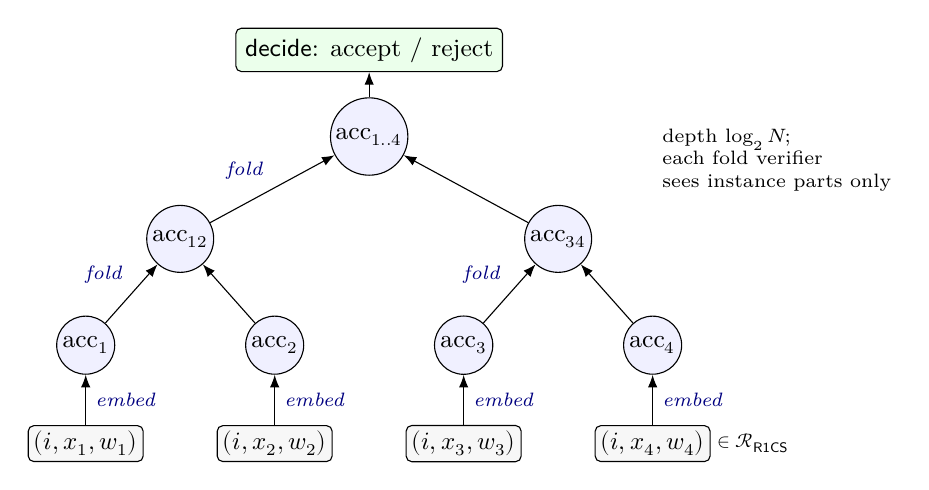
\begin{tikzpicture}[
  every node/.style={font=\small},
  leaf/.style={draw,rounded corners=2pt,fill=black!3,inner sep=2pt},
  acc/.style={draw,circle,inner sep=1.2pt,fill=blue!6},
  op/.style={font=\scriptsize\itshape,text=blue!50!black},
  arr/.style={-{Latex[length=1.6mm]}}]
\foreach \j in {1,...,4} { \node[leaf] (r\j) at (2.4*\j,0) {$(i,x_{\j},w_{\j})$}; }
\node[font=\scriptsize,anchor=west] at (10.3,0) {$\in\Rrcs$};
\foreach \j in {1,...,4} { \node[acc] (a\j) at (2.4*\j,1.25) {$\mathrm{acc}_{\j}$}; \draw[arr] (r\j) -- node[op,right]{embed} (a\j); }
\node[acc] (b1) at (3.6,2.6) {$\mathrm{acc}_{12}$};
\node[acc] (b2) at (8.4,2.6) {$\mathrm{acc}_{34}$};
\draw[arr] (a1) -- node[op,above left]{fold} (b1); \draw[arr] (a2) -- (b1);
\draw[arr] (a3) -- node[op,above left]{fold} (b2); \draw[arr] (a4) -- (b2);
\node[acc] (c) at (6,3.9) {$\mathrm{acc}_{1..4}$};
\draw[arr] (b1) -- node[op,above left]{fold} (c); \draw[arr] (b2) -- (c);
\node[draw,rounded corners=2pt,fill=green!8] (d) at (6,5.0) {$\mathsf{decide}$: accept / reject};
\draw[arr] (c) -- (d);
\node[align=left,font=\scriptsize,anchor=west] at (9.6,3.6) {depth $\log_2 N$;\\ each fold verifier\\ sees instance parts only};
\end{tikzpicture}
\caption{A 2-to-1 accumulation tree for $N=4$ R1CS instances. Each edge is a reduction of
knowledge; the cost of recursion is the fold verifier's, and the decider runs once.}
\label{fig:bg-tree}
\end{figure}

\paragraph{Accumulation without homomorphism.} Group-based folding (Nova and successors
\cite{KST22-Nova,KS24-HyperNova,BC23-ProtoStar,EG23-ProtoGalaxy,NDCTB24-Mangrove}) relies on
additively homomorphic commitments and is not post-quantum. B\"unz, Mishra, Nguyen and Wang give
accumulation from any linear code and Merkle commitments in the ROM \cite{BMNW24}. A
spot-checked linearity test only guarantees that the new accumulator is $\delta$-close to the
claimed combination, so each extraction step loses $\delta$. Soundness is therefore proven only up
to a fixed depth $d$, with a decider family $\mathsf{D}_0\subseteq\dots\subseteq\mathsf{D}_d$, and
there is a concrete attack once $d\delta$ exceeds the unique-decoding radius. \emph{Arc}
\cite{BMNW25-Arc} removes the depth bound for RS codes, with $2\lambda/\log(1/\rho)$ Merkle
openings per input and accumulation up to the list-decoding radius $1-\sqrt\rho$. \emph{WARP}
\cite{BCFW25-WARP} achieves linear-time accumulation for any linear code with MCA, extracting by
erasure correction with the per-round backward extractor of \cref{def:bg-rbrks-warp}. \emph{FICS
and FACS} \cite{BMMS25-FICSFACS} accumulate via code switching with linear-time codes in the
unique-decoding regime; WARP notes that FACS lacks a straight-line extractor for codes not known
to have an efficient error-tolerant decoder. Lattice-based folding
\cite{BC24-LatticeFold,BC25-LatticeFoldPlus} is the other post-quantum route. The deciders of Arc
and WARP are linear in the accumulated instance; recursion.fast admits such deciders, bounded only
by the fuel and amortised in the T2 score (\cref{subsec:rec-score}).

\paragraph{Why recursive soundness is not a theorem in the ROM.} A random-oracle SNARK has a
straight-line extractor that reads the prover's query log, and composing straight-line extractors
costs only additive time. Recursion, however, needs a SNARK for the statement ``$\Vrf^H$ accepts'',
a relation that \emph{itself queries the oracle}. Barbara, Chiesa and Guan prove that such
\emph{relativized} succinct arguments do not exist in the ROM, even interactive ones with
computational soundness \cite{BCG24-RelROM}. Practice therefore replaces $H$ by a concrete hash
inside the circuit and \emph{assumes} that the instantiated scheme is extractable. Under that
assumption, standard-model PCD theorems cover only constant depth, because a recursive extractor
of size $|\tilde\Prv|^c$ per layer costs $|\tilde\Prv|^{c^d}$ at depth $d$
\cite[Rmk.~5.3]{BCMS20}. A 2-to-1 tree over $N$ leaves has depth $\log_2N=\omega(1)$. The known
ways around this either change the oracle model or are heuristic:
\begin{itemize}[nosep]
\item \emph{Arithmetized oracles.} Relativized SNARKs exist in signed, low-degree and arithmetized
  random-oracle models, and PCD for arbitrary depth follows in the AROM \cite{CCS22,CCGOS23-AROM}.
  These models are costly to instantiate and unused in practice.
\item \emph{Straight-line PCD bounds.} If a relativized argument has a straight-line extractor
  with error $\kappa_{\mathrm{ARG}}(\lambda,q,s)$ and time $t_{\mathrm{ARG}}$, PCD over $N$ nodes
  has error $\kappa_{\mathrm{ARG}}(\lambda,q,s+O(N\cdot t_{\mathrm{ARG}}))$, with no dependence on
  depth \cite{CGSY24}. For hash-based PCD this rests on a non-succinct idealisation, so it is
  heuristic evidence, not a proof.
\end{itemize}
leanerVM, the Lean formalisation of leanVM, records this as its open problem T6 (``recursive
CTE''). Its inner knowledge-soundness theorems live in the ROM, but its outer recursion-topology
argument composes plain-model extractors, and no justified interface connects the two. It forbids
a global bridging axiom and keeps the end-to-end theorem as a target schema.\footnote{\repo{leanerVM@8aaf8a0},
\path{README.md:35-38}; \path{docs/architecture.md:297-350}.}

\begin{takeaway}[Consequence for the batcher]
What can be proved today is the \emph{one-step} property: completeness and RBR-KS of the
interactive embed, fold and decide reductions in the information-theoretic model, with an
explicit error. By composition, a tree of fixed shape then has an explicit error sum. Soundness of
the deployed recursive SNARK is a named deployment assumption. It is never a hypothesis of a
competition theorem, and the tree depth must be declared and enforced.
\end{takeaway}

%-----------------------------------------------------------------------------------------------
\subsection{Lean~4, VCVio and ArkLib for cryptographers}\label{subsec:bg-lean}

\paragraph{What a kernel-checked proof certifies.} Lean~4 \cite{MU21-Lean4} is a dependently typed
functional language whose propositions are types and whose proofs are terms. Elaboration (tactics,
automation, macros) produces a term, and a small \emph{kernel} type-checks it. A theorem is
accepted iff its proof term type-checks against its statement in an environment of prior
declarations. A kernel-checked proof therefore certifies exactly the \emph{elaborated statement}
relative to the definitions it mentions and the axioms in its dependency closure. It says nothing
about whether those definitions mean what the reader thinks. This is the key point for
cryptographers: \emph{the proof is trustworthy; the statement must be audited}.

\paragraph{The trusted computing base.}
\begin{itemize}[nosep]
\item \emph{Kernel.} Lean's kernel, optionally rechecked by independent kernels (nanoda, lean4lean)
  on an exported environment \cite{lean4export,nanoda,carneiro2024lean4lean}. Kernels are not
  infallible: Lean~4.34.0 fixed three proof-of-\lean{False} routes \cite{lean4340}, and a
  nested-inductive projection bug that yielded an axiom-free $0=1$ was also accepted by nanoda
  \cite{brossard2026leanproj}. Kernel diversity is defence in depth, not proof.
\item \emph{Axioms.} Mathematics in Mathlib uses three: \lean{propext} (propositional
  extensionality), \lean{Quot.sound} (quotients) and \lean{Classical.choice} (global choice, hence
  excluded middle). \lean{\#print axioms t} lists the axioms in the closure of \lean{t}. Any other
  axiom, including a user-declared \lean{axiom}, is a hole.
\item \emph{\lean{sorry}} closes any goal by the axiom \lean{sorryAx}. It is the standard
  placeholder for an unfinished proof and is detected by the axiom audit, transitively: a theorem
  that uses a sorried lemma inherits \lean{sorryAx}.
\item \emph{\lean{native\_decide}} evaluates a decision procedure with the compiler rather than the
  kernel, through the axiom \lean{Lean.ofReduceBool}. It thereby trusts the compiler and every
  \lean{@[implemented\_by]} and \lean{@[extern]} annotation in scope, so competitions refuse it.
  Kernel-checked \lean{decide} is permitted but slow.
\end{itemize}

\paragraph{Definitional versus statement-level attacks.} Attacks on a proof checker
(\lean{sorry}, extra axioms, compiled evaluation, environment manipulation by metaprograms, kernel
bugs) are handled by tooling. The Lean FRO's \emph{comparator} \cite{comparator} builds a trusted
challenge and the candidate in a sandbox, exports both, checks that each target theorem has the
same type and that every constant its statement uses is identical, audits axioms, and replays the
candidate in a fresh kernel. Attacks on the \emph{statement} are not handled by any checker. They
include vacuous hypotheses, a definition left open (a \emph{definition hole}, which comparator
matches only by name and type), an error bound that is trivial at the chosen parameters, and an
existentially chosen object that makes a property easy. Comparator's documentation states that
definition holes must be checked by an additional, possibly human, verifier. The real failures of
Lean-checked competitions and zkVM verification efforts so far were of this second kind
(\cref{sec:prior}).

\paragraph{VCVio: oracle computations.} VCVio \cite{tuma2024vcvio,tuma2026vcvio} models a
probabilistic oracle algorithm as a \emph{free monad} over an oracle specification: a program is a
finite tree whose nodes are queries and whose leaves are results.

\begin{leancode}
-- VCVio: oracle computations and probabilistic programs
def OracleComp (spec : OracleSpec ι) := PFunctor.FreeM spec.toPFunctor
abbrev ProbComp := OracleComp unifSpec          -- only uniform coin queries
-- simulateQ impl oa : interpret every query of `oa` by `impl` (e.g. a lazy random oracle)
-- Pr[ event | oa ] : probability of `event` under the output distribution (in ℝ≥0∞)
\end{leancode}

\noindent An adversary is an arbitrary term of type \lean{OracleComp spec α}. Its local computation
is free and unbounded; only queries carry information, and a query budget is a predicate on the
tree (\lean{IsQueryBound}). A random oracle is a stateful query implementation with a cache, and
\lean{simulateQ} runs a program against it. Probabilities are \lean{ENNReal}-valued. Failure is
added with \lean{OptionT}, and the probability notation counts failure mass as not satisfying the
event, so verifier aborts count as rejections.

\paragraph{ArkLib: protocols and security.} ArkLib \cite{arklib2026} builds on VCVio. A protocol is
described by its message schedule:

\begin{leancode}
structure ProtocolSpec (n : ℕ) where
  dir : Fin n → Direction          -- P_to_V (message) or V_to_P (challenge)
  «Type» : Fin n → Type            -- type of the i-th message
structure Verifier (oSpec) (StmtIn StmtOut : Type) (pSpec : ProtocolSpec n) where
  verify : StmtIn → FullTranscript pSpec → OptionT (OracleComp oSpec) StmtOut
\end{leancode}

\noindent A \lean{Reduction} pairs a prover with such a verifier. An \lean{OracleReduction} lets
the verifier reach prover messages and input oracles only through queries, and a \lean{Proof} is a
reduction whose output statement is \lean{Bool}. The verifier does not sample its own randomness:
the execution draws challenges uniformly, so every protocol is public-coin. Every security
definition is parameterised by the implementation of the shared oracle \lean{oSpec}; the
information-theoretic setting is \lean{oSpec = []ₒ}. The definitions of completeness, soundness,
straight-line knowledge soundness, RBR soundness and RBR-KS (averaged, worst-case, one-shot and
named-extractor forms) contain no \lean{sorry}. Most \emph{general theorems} relating them are
\lean{sorry}, however. This includes RBR-KS $\Rightarrow$ KS, every generic sequential-composition
and context-lifting security theorem, the SR implications and Fiat--Shamir completeness. ArkLib has
no BCS transform and no Merkle trees; VCVio has the latter. 281 declarations are transitively
tainted by \lean{sorryAx} at the examined commit.\footnote{\repo{ArkLib@db7005f},
\path{scripts/axiom_baseline.json}; definitions in
\path{ArkLib/OracleReduction/Security/Basic.lean} and \path{RoundByRound.lean}; sorried theorems in
\path{.../Security/Implications.lean:49,79,193} and
\path{.../Composition/Sequential/Append/Security.lean:47-94}.} Two consequences for a
contract follow. Importing ArkLib definitions is safe, provided an axiom audit rejects any use of
the sorried theorems. Concretely, a toy ``send the witness'' R1CS proof shows knowledge soundness
through \lean{rbrKnowledgeSoundness\_implies\_knowledgeSoundness} and compiles, but
\lean{\#print axioms} reports \lean{sorryAx}. And the contract must fix the oracle model and the
error budget itself, because both are parameters chosen by whoever proves the theorem.

The worst-case RBR-KS of \cref{def:bg-rbrks-warp} reads, in the counting form adopted by the design
(local restatement, with a proved bridge to ArkLib's
\lean{rbrKnowledgeSoundnessWorstCaseWith}):

\begin{leancode}
def KSF.Bad (kSF : KSF relIn relOut V E) (i : pSpec.ChallengeIdx) (s)
    (tr : pSpec.Transcript i.1.castSucc) (c : pSpec.Challenge i) : Prop :=
  ∃ w, ¬ kSF.toFun i.1.castSucc s tr (E.extractMid i.1 s (tr.concat c) w)
       ∧ kSF.toFun i.1.succ s (tr.concat c) w
def RbrKS (kSF : KSF relIn relOut V E) (ε : pSpec.ChallengeIdx → ℝ≥0) : Prop :=
  ∀ s i (tr : pSpec.Transcript i.1.castSucc),
    (Nat.card {c // kSF.Bad i s tr c} : ℝ≥0) ≤ ε i * Fintype.card (pSpec.Challenge i)
\end{leancode}

\noindent The statement involves no \lean{Pr}, \lean{simulateQ} or random-oracle cache: ``at most
an $\eps_i$-fraction of challenges is bad, for every prefix.'' Finiteness of challenge types is
required, because \lean{Nat.card} of an infinite type is $0$, a classic vacuity trap.

\paragraph{What ``information-theoretic knowledge soundness'' means in Lean.} ArkLib's extractors
are Lean functions with no running-time or query bound. ArkLib itself constructs extractors by
\lean{Classical.choose}. Take the extractor that returns a chosen valid witness whenever one
exists. Then straight-line KS collapses to soundness with respect to $L(\R)$, and RBR-KS collapses
to RBR soundness with the same errors. On finite witness spaces a computable brute-force extractor
does the same, so ``computable'' is no remedy. For R1CS this is a weakening, not a vacuity:
unsatisfiable instances exist, so RBR soundness remains a non-trivial property of the verifier, and
it is the property deployed STARKs are analysed for. Extractor \emph{efficiency} becomes
load-bearing in two places. One is the compiled knowledge claim, because the BCS extractor runs the
IOP extractor. The other is the recursion heuristic, because the CGSY24 bound contains
$N\cdot t_{\mathrm{ARG}}$. A contract that wants computational content must therefore demand a
named, executable extractor (the \lean{\ldots With} forms) and, at a higher level, a cost bound for
it.

% Provenance: copied from the design workspace CambridgePQ/recursion.fast, `report/sections/04-prior-competitions.tex`, on 2026-10-19. Read-only copy; the source is authoritative.
% 04-prior-competitions -- written by W1
\section{Prior Lean-checked competitions}\label{sec:prior}

Three live competitions score submissions by a Lean proof checked against a trusted
contract: ots.golf \cite{otsgolf2026}, sig.golf \cite{siggolf2026} and the Proximity Prize on
better.codes \cite{proximityprize2026}. recursion.fast inherits their machinery and their bugs, so
this section records how they are built, what checking them costs, and what went wrong. Facts come
from the pinned checkouts listed in \cref{tab:prior-overview}. Times marked ``measured'' were taken
on this study's 32-core, 62\,GB machine. That machine was shared with other builds, and the
sandbox tool landrun was replaced by comparator's non-sandboxing shim, so wall-clock figures are
upper bounds on proof-checking time and exclude sandbox overhead.

\begin{table}[t]
\centering\small
\begin{tabularx}{\linewidth}{@{}>{\raggedright\arraybackslash}p{2.35cm}>{\raggedright\arraybackslash}X>{\raggedright\arraybackslash}X>{\raggedright\arraybackslash}X@{}}
\toprule
& ots.golf (RISC-V track) & sig.golf & Proximity Prize \\
\midrule
Checkout & \repo{ots.golf-dev@8b140a9}; Lean v4.33.1 & \repo{sig.golf-dev@eaa0c7f}; Lean v4.33.1 & \repo{proximity-prize@ed2b68c}; Lean v4.32.2, ArkLib \texttt{e651978} \\
Object & hash-based one-time signature & stateless hash-based signature & threshold radius of a fixed toy IOP \cite[§6]{ABF26} \\
Score & proved cycle bound on \emph{every} run (record 341) & $S\times C$: signature bytes $\times$ proved honest-verify cycles (70{,}986{,}432) & certified bits $B/100$: lower 68.15, upper 116.13 \\
Trusted Lean & 1{,}625 lines / 623 code (RISC-V path $\approx$220 code) + $\approx$1{,}500 code lines of riscv-zkvm & 712 lines / 412 code + $\approx$4.3k-line riscv-zkvm import closure & 290 lines (3 files), of which $\approx$30 are the scored statements; ArkLib/VCVio closure \\
Machine & Harvard RV64IM subset (code as \lean{List Instr}, five W-ops), \texttt{HASH}/\texttt{HALT} syscalls & raw 32-bit words, contract decoder and all W-ops, \texttt{HASH}/\texttt{HALT} & none \\
Cost model & 1 cycle/instruction; \texttt{HASH} 1 per started 512-bit block & 1; \texttt{MUL}/\texttt{DIV}/\texttt{REM} 4; \texttt{HASH} 8 per 64-byte block; witness $\lceil W/256\rceil$ & n/a \\
Checker & comparator \texttt{c0c5a52}, nanoda off & comparator \texttt{c0c5a52}, nanoda off & comparator \texttt{777e7f5}, patched to \texttt{leanchecker} \\
Limits & 1{,}200\,s, 24\,GiB, 200 files, 16\,MiB & 4\,h, 24\,GiB, 2 CPUs, 1{,}000 files, 16\,MiB & 4\,h, 24\,GiB, 4 vCPU, 1{,}000 files, 16\,MiB \\
\bottomrule
\end{tabularx}
\caption{The three Lean-checked competitions. All three permit exactly the axioms
\lean{propext}, \lean{Quot.sound} and \lean{Classical.choice} and refuse
\lean{native\_decide}.}
\label{tab:prior-overview}
\end{table}

\subsection{ots.golf}\label{subsec:prior-ots}

ots.golf asks how cheaply a hash-based one-time signature can be verified. Every score is a
proved bound; there is no trusted emulator in the scoring path. Five tracks share one cost model:
a single random oracle on bit strings, charged one compression per started 512-bit block. They are
a lower bound for whole-word DAG schemes, compressions, RISC-V cycles, hinted RISC-V cycles and
leanISA cycles. Records at the examined submissions commit were 90, 86, 341, 310 and 1088
respectively.\footnote{\repo{ots.golf-submissions@30cff14}, \path{records.json};
\repo{ots.golf-dev@8b140a9}, \path{challenges.json:48-183}.}

\paragraph{Contract and statement.} Security is concrete and stated in VCVio (\cref{subsec:bg-lean}).
For every adversary and every \emph{pathwise} query budget $B$ of the whole experiment, honest
parties included, the forgery probability is below $B/2^{127}$. The RISC-V track's
\lean{Certificate} bundles four clauses.
\begin{itemize}[nosep]
\item \lean{admissible}: perfect correctness, determinism, size limits and budgets of $2^{20}$
  for key generation, signing and verification.
\item \lean{secure}: the bound above.
\item \lean{implements}: the machine's run equals the Lean verifier as an \emph{equality of
  oracle-computation trees} on every raw input. This forces the same queries and the same decision
  and excludes traps and fuel exhaustion.
\item \lean{cycles}: a bound over every execution, accepting or rejecting.
\end{itemize}
A separate theorem caps the image below 1\,MiB.\footnote{\repo{ots.golf-dev@8b140a9},
\path{formal/OptimalOTS/Riscv.lean:18-45}, \path{formal/OptimalOTS/OracleAlgorithm.lean:63-65,117-125}.}
The machine is a 79-code-line wrapper around the riscv-zkvm hand model. Its pieces are a Harvard
image (\lean{List Instr} plus data bytes), a raw-input loader with a length sentinel, the
\texttt{HASH} and \texttt{HALT} syscalls selected by register \texttt{t0}, and a fuel-indexed
\lean{execute} in \lean{OracleComp}. The admitted instruction set is a strict subset of RV64IM:
of the W-suffixed 32-bit operations it contains only five, which matters for
32-bit word arithmetic (for example 31-bit prime fields). The submitted \lean{submission} is a comparator \emph{definition hole}, and the
certificate pins it so completely that any term of the stated type is a legitimate win. The hinted
track adds a prover-chosen ``view''. Its four clauses are \lean{Sound} (no view makes the machine
accept what the specification rejects, on every coherent oracle assignment), \lean{Faithful} and
\lean{Expands} (honest views reach the specification's decision), and a cycle bound over \emph{all}
views. Together they are the template for a verifier that reads an untrusted proof.

\paragraph{Pipeline.} The pipeline is generic and reusable. It refuses to run as root and requires
Landlock. It exports only the submission root, as flat regular files read at blob level. It checks
the protected-file pin (the contract id is the SHA-256 of the pin file) and applies an import
policy of exact modules for the contract and prefixes for Mathlib and VCVio. It clones a prebuilt
\texttt{.lake} cache and deletes any stale submission or challenge oleans. It renders the claim
into the challenge stub. Finally it runs comparator under a transient systemd unit with memory and
runtime limits, a syscall filter, private PID, IPC and device namespaces, and a cleared
environment. The audit document is explicit that header checks do not constrain runtime module
loads by metaprograms; that guarantee rests on comparator.\footnote{\repo{ots.golf-dev@8b140a9},
\path{verifier/verify.py:156-628}, \path{docs/AUDIT.md:23-29}.}

\paragraph{Measured cost.} Checking the 341-cycle record end to end took 1{,}516\,s
(25\,min\,15\,s; measured), above the 1{,}200\,s production limit, with a 12.9\,GB peak per
process. The solution build was about 1{,}230\,s of this, and its critical path was one 176-line
module (472\,s) containing four \lean{decide +kernel} proofs over all 5{,}328 signature-bit
positions. The submitters report 836\,s hosted for the 358-cycle predecessor. A compressions-track
predecessor timed out on the hosted runner at 1{,}230.6\,s.\footnote{\repo{ots.golf-submissions@30cff14},
\path{formal/Submissions/UpperRiscv/Payload.lean:41-44}, \path{.../UpperRiscv/NOTES.md:473},
\path{.../UpperCompressions/NOTES.md:220-246}.} Record roots are 20--100k lines, and OTS-sized
programs already have less than $2\times$ headroom against the time limit.

\subsection{sig.golf}\label{subsec:prior-sig}

sig.golf, run by Yukon (Eigen Labs) with the Ethereum Foundation, asks for a stateless hash-based
signature minimising $S\times C$: signature bytes times the proved maximum honest verification
cycles. A submission consists of four RV64IM images (keygen, sign, expand, verify), sizes and
buffer offsets, and Lean proofs. The 412-code-line contract defines one semantic object,
\lean{execute} in \lean{OracleComp HashSpec}. It is read three ways: against a lazy random oracle
(completeness), against an arbitrary fixed hash function (worst-case cost and termination), and
inside a counted oracle (security). The \lean{Certificate} has six fields.
\begin{itemize}[nosep]
\item \lean{admission}: decidable size and layout checks.
\item \lean{completeness}: success probability at least $1-2^{-128}$ for every secret key and
  \emph{all $2^{256}$ messages simultaneously}.
\item \lean{compressionBudgets}: exponential-moment budgets
  $\mathbb{E}[2^{N/B}]\le2$, which allow grinding while bounding tails.
\item \lean{verificationCycles}: $C$ bounds every successful honest run under every fixed oracle.
\item \lean{security}: $\Pr[\mathsf{won}\wedge\mathsf{calls}\le Q]\le Q/2^{127}$.
\item \lean{termination}: fewer than $2^{32}$ cycles on all typed inputs.
\end{itemize}
The upstream decoder models only two of the ten W-ops, so the contract decodes them itself.\footnote{\repo{sig.golf-dev@eaa0c7f},
\path{SigGolf/Statements.lean:12-60}, \path{SigGolf/Riscv.lean:66-67,150-154,204-224}.}

\paragraph{The accepted submission} (SPHINCS+ with PORS+FP, $S=6061$, $C=11{,}712$) has 958 files
and 154{,}526 lines, near the caps of 1{,}000 files and 16\,MiB. Of these, 59\% is the abstract
security argument in VCVio, 22\% is RISC-V refinement, 10\% is generated image data and 1\% is a
1.8k-line transfer from an older contract. Refinement is an equality of oracle computations,
proved with a custom verified symbolic executor whose results are certified by kernel reduction
(\lean{Eq.refl}), never by \lean{native\_decide}. The verify image has 145{,}952 instructions, of
which 72{,}960 are NOP padding: code size is free up to the 1\,MiB cap, so agents spend it on
unrolling. Measured: the candidate build took 16\,min\,07\,s on 32 cores (2.83 CPU-hours, 5.6\,GB
peak per process), and comparator's single-threaded export, comparison and kernel replay took a
further 23\,min\,25\,s. Extrapolated to the official two CPUs, that is about 1.7--1.9\,h of the
4\,h budget.\footnote{Measured in this study (probe \texttt{sig-golf-build}); breakdown from
\repo{sig.golf-dev@eaa0c7f}, \path{submission/SigGolfCandidate/}.}

\subsection{The Proximity Prize (better.codes)}\label{subsec:prior-proximity}

Yukon and zkSecurity's Proximity Prize differs from the two golf competitions: the protocol is
fixed and only a number is contested. That number is a threshold radius $\delta^\ast$ of the
ABF26 toy IOP \cite{ABF26} instantiated with an interleaved RS code over the sextic extension of
KoalaBear: $n=2^{18}$, message length $2^{20}$, interleaving 8, rate $1/2$ and $t=128$ spot
checks. The lower track proves the combination-round error \lean{certifiedGammaError} at most
$2^{-128}$ at radius $P/Q$ and claims $B$ with $(1-\delta)^{128}\le2^{-B/100}$. The upper track
proves the winning-set density above $2^{-128}$ on the whole suffix $[\delta^\ast,\delta_C)$,
which avoids assuming an unproved monotonicity lemma. The README states that the score ``is not a
full-protocol security claim''. Each claim is a \lean{structure \ldots : Prop} with three named
fields, and its scalars are rendered from strictly parsed text files into the challenge
type.\footnote{\repo{proximity-prize@ed2b68c}, \path{ProximityPrize/Benchmark/TargetLower.lean:28-57},
\path{TargetUpper.lean:32-52}, \path{README.md:15-16}.} The trusted Lean contract is three
files of 290 lines, unchanged for six weeks and about 125 validated submissions. All game
semantics sits in ArkLib behind one bridge theorem (certified error $\Rightarrow$ knowledge
soundness of an executable, named straight-line extractor). The organisers audited that theorem
once, and ArkLib's \lean{sorry}s are kept outside the protected import cone by the axiom audit.

\paragraph{Pipeline and cost.} A textual audit, run after stripping comments and string
interiors, rejects module-system headers and metaprogramming, such as the commands
\texttt{\#eval}, \texttt{elab}, \texttt{macro} and \texttt{addDecl} and the attribute
\texttt{implemented\_by}. Comparator runs under landrun and systemd, but in patched form
(63 lines): its fresh-environment kernel replay was replaced by a sandboxed \texttt{leanchecker}
pass over the untrusted modules. Comparator's replay ignored declaration-local recursion limits
and could not replay CompPoly's checked irreducibility certificate for the extension
field.\footnote{\repo{proximity-prize@ed2b68c}, \path{setup.sh:41-46},
\path{scripts/check-submission-imports.sh:141-145}.} The trusted import closure has 5{,}398
modules and 495{,}846 constants, and loading it costs about 4\,GB and 9\,s per process. Measured:
setup took 615\,s on 32 shared cores. The baselines checked in 15\,s and 33\,s on 4 cores. The
current upper submission (2{,}256 lines) took 126\,s. The current lower submission (153 files,
14.7\,MB, $\approx$13k \lean{decide} uses) had not finished after 50\,min, with 92 of 153 modules
built. Agent-optimised submissions grow to the resource ceilings, so the ceilings, not the
contract, set the check time.

\subsection{Other precedents}\label{subsec:prior-other}

zk.golf (zkSecurity) asks for Clean circuits minimising allocations and constraints under a formal
interface. It requires soundness \emph{and} completeness (its authors note that completeness is
what blocks the ``unsatisfiable circuit is sound'' win), a proof that the circuit is R1CS, and
cost proofs. It is checked by comparator with per-challenge permitted axioms and a 1{,}200\,s limit
\cite{dellimmagine2026zkgolf}. Yukon hosts further challenges (precompile.fast, SNARK.fast, and
others) under a common model: the challenge creator supplies the verifier and the baseline, and a
deterministic gate runs before merge \cite{yukon2026}. Of these, only the three above score by a
Lean theorem about a protocol.

\subsection{Vacuity bugs and lessons learned}\label{subsec:prior-lessons}

Every serious failure observed so far was a \emph{specification} failure: the statement was weaker
than intended, and no checker could notice.
\begin{table}[tp]
\centering\small
\begin{tabularx}{\linewidth}{@{}>{\raggedright\arraybackslash}p{5.4cm}>{\raggedright\arraybackslash}X@{}}
\toprule
Lesson & Consequence for recursion.fast \\
\midrule
(1) Concrete bounds that count honest work become vacuous without caps &
  The security statement is information-theoretic, with no query budget. Cost is a separate
  proved theorem on the machine. Every free resource is capped: code and data at 1\,MiB, the
  verification key at $2^{10}$ elements, the accumulator statement (cost model; security section). \\
(2) ``$=0$'' soundness with hashing is unsatisfiable &
  Security is RBR-KS with a contract-fixed error cap in counting form; the L1 machine has no
  \texttt{HASH} syscall (protocol model). \\
(3) Decision agreement does not transfer costs &
  The machine--specification link \lean{Agrees} is decision-only, and no cost is transferred from
  the specification; cycles and query charges are read off the machine (architecture; cost
  model). \\
(4) Free lookup tables & Proved caps on image, key, tape, oracle lengths and rounds (cost model). \\
(5) Candidate code on the trust path & The binding rule: images are raw files rendered by the
  trusted harness into the challenge as literals and loaded unchanged by the trusted emulator; no
  candidate code is executed (architecture). \\
(6) Heavy certificates break replay & The field $K=\mathrm{GF}(2^{64})$ is restated in about
  25 core-only lines. Its irreducibility certificate (CompPoly's kernel-checked Rabin test) stays in
  the untrusted library and replays under unpatched comparator in 101\,s; this replay is a CI test
  (protocol model; reproducibility appendix). \\
(7) Sorried instances and lemmas in libraries & Exact-module imports of ArkLib's vocabulary only;
  axiom whitelist with negative controls; sorried general theorems never trusted (Lean
  contract). \\
(8) Statement rewriting & comparator statement comparison against a challenge elaborated only in
  the trusted environment. \\
(9) Vacuous theorems & Kernel-checked negative controls in the trusted
  repository: accept-all is not RBR-KS, reject-all is not complete, the error cap is load-bearing
  (security section). \\
(10) Library-level traps, incl.\ truncation and declared errors & Finite, nonempty challenge types;
  numeral caps; per-round error cap $\eps_i\le2^{-128}$ fixed by the contract (security section). \\
Completeness blocks trivial wins (zk.golf) & Perfect completeness for every challenge vector is
  part of every certificate (security section). \\
Definition holes are gameable & The certificate pins the submission hole so that any inhabitant
  is a legitimate win (Lean contract). \\
(11) Churn and check time & Freeze contract and toolchain before launch, with a record-porting
  procedure. Budgets of 3\,h, 8 CPUs and 48\,GiB are set from measurements, the baseline checks in
  $\approx8$\,min warm and 20--25\,min cold, and an admitted, untrusted RISC-V proof library is provided (benchmark; issues). \\
\bottomrule
\end{tabularx}
\caption{Lessons from prior competitions and the design decisions they motivate. Decisions are
referred to by name; their sections give the details.}
\label{tab:prior-lessons}
\end{table}

\begin{enumerate}[nosep,label=(\arabic*)]
\item \emph{Cost-cap vacuity (ots.golf, commit \texttt{30e33a7}, 2026-09-21).} The security bound
  $B/2^{127}$ counts honest queries. A verifier hashing a single $2^{137}$-bit input costs $2^{128}$
  on every path, so every valid $B$ gives $B/2^{127}\ge2$, and a scheme with a fixed key and empty
  signatures was ``secure'' and forgeable with probability 1. This was checked in Lean against
  the old contract and fixed by capping verification cost at $2^{20}$. Only the leanISA track was
  exposed, because the RISC-V track's tree equality charges the verifier's hashing in
  cycles.\footnote{\repo{ots.golf-dev@8b140a9}, \path{formal/OptimalOTS/OracleAlgorithm.lean:57-62};
  \path{docs/AUDIT.md:76-84}.}
\item \emph{Unsatisfiable exact soundness (ots.golf leanISA).} Soundness there is
  ``\lean{probTrue \ldots{} = 0}'', i.e.\ no accepting run on any coherent oracle assignment.
  Binding the long public statement through a digest would make it unsatisfiable for \emph{every}
  program, because collisions exist on some assignment. The contract instead idealised the
  boundary and charged a fixed 120 cycles for it.\footnote{\repo{ots.golf-dev@8b140a9},
  \path{formal/OptimalOTS/LeanIsaMachine.lean:264-318}.} Statements involving hashing must be
  probabilistic bounds, not ``$=0$''.
\item \emph{Decision agreement does not transfer costs.} A specification that queries $H(x)$
  twice and a machine that queries it once decide identically under a cache. Costs must therefore
  be read off the machine.
\item \emph{Free lookup tables.} Proved size caps were added after launch (commit \texttt{b38f3c5}:
  RISC-V image below 1\,MiB; leanISA \lean{maxProgramLogSize}, called ``load-bearing, not
  hygiene''). The OTS record image is mostly jump tables, and sig.golf's verify image uses 57\% of
  its cap.
\item \emph{Candidate code on the trust path (sig.golf, commit \texttt{bb5ae34}, 2026-09-29).} The
  verifier used to evaluate the images with \lean{\#eval} and publish their digests. This was
  removed because it ran candidate-controlled compiled code (\lean{implemented\_by}, \lean{\#eval}
  overrides, files written at build time). The scores never depended on the digests.
\item \emph{Checker incompatibility (Proximity Prize).} A heavy computational certificate in the
  trusted cone (extension-field irreducibility) and declaration-local recursion limits broke
  comparator's replay, forcing a locally patched checker.
\item \emph{Sorried instances in dependencies.} Clean carries a sorried
  \lean{Fact (Nat.Prime BN254\_PRIME)} instance that typeclass synthesis can pick up ``with no
  syntactic trace''. ots.golf therefore admits leanerVM modules only as exact imports, with the
  axiom audit as backstop.
\item \emph{Statement rewriting by agents.} In a 100-agent research swarm, agents used
  \lean{local notation} to redefine names in theorem statements (for example
  \lean{LinearIndependent}) \cite{paglieri2026swarm}. A textual check misses this. Comparing
  elaborated kernel types against a trusted challenge, as comparator does, catches it.
\item \emph{Vacuous theorems in zkVM verification.} An EF audit of SP1 Hypercube's Lean RV64
  verification found 51 of 62 claimed opcodes complete and correct. \texttt{SLTI}'s theorem was
  vacuous (contradictory hypotheses), several loads used width-1 specifications, all loads depended
  on \lean{sorry}, and \texttt{JALR} omitted \texttt{\&\,\textasciitilde1}
  \cite{gunton2026sp1bug}.
\item \emph{Library-level vacuity traps.} ArkLib documents that running the extractor inside the
  outer failure monad let an always-failing extractor discharge knowledge soundness at error $0$.
  The Proximity Prize guards \lean{ENNReal.toNNReal} and \lean{toNat}, which silently send $\infty$
  to $0$. leanerVM records that a declared error of $1$ makes a knowledge theorem hold of a phase
  that checks nothing.
\item \emph{Churn and check time.} ots.golf changed its protected-file pin 46 times in its first
  ten days. sig.golf's winner carries a 1.8k-line proof transferring it from an older contract.
  Submissions were rejected for exceeding time limits after successful builds, and once for a
  local \lean{autoImplicit} setting that differed from the pinned project's.
\end{enumerate}


% Provenance: copied from the design workspace CambridgePQ/recursion.fast, `report/sections/05-brief-review.tex`, on 2026-10-19. Read-only copy; the source is authoritative.
\section{Critical review of the brief}\label{sec:brief-review}

The brief~\cite{recursionfastbrief} fixes the intent of recursion.fast: a competition in which
untrusted agents submit SNARK verifier specifications for arbitrary R1CS, as RISC-V programs with an
honest prover and a two-to-one \emph{batcher}, together with Lean~4 proofs of knowledge soundness and
completeness, scored by a cost function that should reward interesting, general verifier architectures
rather than trivial or overfitted ones. The intent is sound and the precedents it names (ots.golf,
sig.golf, the Proximity Prize; \cref{sec:prior}) show that the format works. Before designing, we
reviewed the brief for ambiguities and missing scope. \Cref{tab:brief-review} lists the twelve points
we found; each is resolved later in the report, and the last column summarises the resolution and
names the decision (blue box) or section that makes it. The four points with the largest
consequences are discussed first.

\paragraph{The objective and the proposed score.} \enquote{As efficient as possible} admits four
readings that pull against each other: final-layer verifier cost, cost of one recursion step, proof
size, and prover time. Lowering the code rate shrinks the first three and raises the fourth; grinding
does the same in the Fiat--Shamir setting. The name of the competition and the brief's
\enquote{ambitious variant} (arithmetise the verifier and measure 2-to-1 recursion) point at the
recursion step, which we adopt as the primary objective (\cref{sec:objectives}). The proposed score,
\enquote{median performance on hash-chain proofs divided by the size of the RISC-V verifier and
batcher programs}, is dimensionally inverted if performance is measured in cycles: dividing a cost by
a size rewards \emph{larger} programs. Any additive or multiplicative size term would also reward
obfuscation and code compression, which no user pays for. Both earlier golf competitions instead cap
program size and do not score it; ots.golf introduced its cap after launch because an uncapped image
is a free lookup table~\cite{otsgolf2026}. We follow them (\cref{sec:cost}).

\paragraph{Succinctness for arbitrary R1CS requires preprocessing.} A verifier that reads the
constraint matrices pays $\Theta(\mathrm{nnz})$ field operations, which is the cost of the trivial NP
verifier. Succinct verification of a \emph{non-uniform} relation requires an indexer that commits to
the circuit once, producing a short verification key and an index oracle that the verifier queries
(holography; \cref{subsec:bg-r1cs}). The brief does not mention an indexer or a verification key. We
add both, cap the key (otherwise it is again a lookup table) and price every access to the index
(\cref{sec:protocol}).

\paragraph{Knowledge soundness does not prevent overfitting.} A verifier specialised to the
benchmark's circuit can remain knowledge-sound, because the extractor may carry the benchmark
witness; overfitting must instead be excluded by a class-uniform cost theorem
(\cref{subsec:bench-hardcode}). Relatedly, Lean extractors have no running-time bound, so knowledge
soundness collapses to soundness (\cref{subsec:sec-extractor}).

\paragraph{The batcher property as stated is completeness only.} A batcher that outputs a fixed
accepting proof, or concatenates, satisfies it; the load-bearing property is knowledge of witnesses
for \emph{both} inputs with a batched object of bounded size (\cref{subsec:rec-critique}). We define
the batcher as an accumulation scheme in the information-theoretic model and state the recursive
deployment, which no random-oracle theorem covers~\cite{BCG24-RelROM}, as a named assumption
(\cref{subsec:rec-cannot}).

\begingroup
\small
\renewcommand{\arraystretch}{1.15}
\begin{longtable}{@{}p{0.03\textwidth}p{0.30\textwidth}p{0.29\textwidth}p{0.30\textwidth}@{}}
\caption{Points raised in the review of the brief and their resolution.}\label{tab:brief-review}\\
\toprule
\# & Point & Why it matters & Resolution \\
\midrule
\endfirsthead
\toprule
\# & Point & Why it matters & Resolution \\
\midrule
\endhead
1 & Objective ambiguous (final verifier, recursion step, proof size, prover) & the four pull in opposite directions & recursion-step cost primary; proof size and prover time as constraints and secondary tracks (\cref{subsec:obj-what}) \\
2 & Score \enquote{performance $\div$ program size} & dimensionally inverted; size terms reward obfuscation & cycles plus a byte charge; hard 1~MiB program cap (COST-1, \cref{sec:cost}) \\
3 & No indexer or verification key & arbitrary R1CS cannot be verified succinctly without preprocessing & holographic model: capped key, priced index oracle (P-1, \cref{subsec:proto-indexer}) \\
4 & Interactive \enquote{proof} vs argument unspecified & succinct interactive proofs for NP need an oracle or commitment model & interactive: public-coin IOP in Lean; BCS and Fiat--Shamir as cited meta-theorems with explicit bounds (P-1, S-4; \cref{subsec:sec-cap}) \\
5 & Honest prover in RISC-V & a proved RISC-V SNARK prover would dwarf sig.golf's 154k-line proof; but prover cost must still be constrained & Lean prover specification for completeness; static prover caps; native prover for record runs (BEN-2, \cref{subsec:arch-badge}) \\
6 & Knowledge soundness does not prevent hard-coding & extractors are existential & class-uniform cost theorem over all R1CS in a class (BEN-1, \cref{subsec:bench-hardcode}) \\
7 & Batcher property is completeness only & concatenation and constant proofs satisfy it & accumulation scheme with knowledge soundness and a size cap; recursion heuristic named (REC-1, REC-2) \\
8 & Security parameters unspecified (field, bits, proven vs conjectured regimes, quantum, zero knowledge) & Lean proofs cannot assume conjectures; several capacity conjectures are now false & binary relation field $\mathrm{GF}(2^{64})$ with challenges in $\mathrm{GF}(2^{192})$, per-round error $\le 2^{-128}$, proven regimes, named hypotheses in a separate track; classical; no ZK (P-3, S-2, S-5) \\
9 & \enquote{Median over millions of runs} & honest verification cost is essentially input-independent; measurements are noisy and gameable & proved worst-case bound, an 18-counter cost vector, over all accepting runs (fast-failing rejections unscored, fuel-capped); measurements as unscored demonstrations (COST-1, BEN-1) \\
10 & Field arithmetic in RV64IM unpriced & the cost model decides which field and which arithmetic wins & contract machine RV64IM+Zbc (carry-less multiply as the only field assist, priced separately); v0.3 per-profile zkVM cost vectors (recursion board) and a latency board; no hash or field syscall on T1 (a field-syscall board T1-F is planned); field fixed by the relation (P-5, COST-1) \\
11 & Toolchain and check-time feasibility & ArkLib and riscv-zkvm pin different Lean versions; real submissions take hours to check & single pinned toolchain with vendored RISC-V model; measured budgets (A-2, \cref{subsec:base-time}) \\
12 & Trusted vs untrusted boundaries & imports with \code{sorry}, Lean-level attacks, harness code & explicit trusted surface, comparator pipeline, axiom whitelist, binding rule (A-1, A-3; \cref{tab:arch-trusted}) \\
\bottomrule
\end{longtable}
\endgroup

\paragraph{Scope added.} Beyond the twelve points, the blueprint covers three topics the brief does
not request but which a deployment needs: Fiat--Shamir statement binding against weak-FS and
generated-R1CS attacks~\cite{BPW12-WeakFS,Fen26-GenR1CS}, and the hash-in-circuit attack
of~\cite{KRS25} as a named deployment assumption (\cref{subsec:sec-fs,subsec:rec-cannot}); the governance of trusted
mathematical hypotheses such as proximity-gap theorems that are published but not yet formalised
(\cref{subsec:sec-hypotheses}); and contract versioning and record revalidation, which both golf
competitions found expensive after launch (\cref{sec:issues}).

% Provenance: copied from the design workspace CambridgePQ/recursion.fast, `report/sections/06-architecture.tex`, on 2026-10-19. Read-only copy; the source is authoritative.
% 06-architecture -- written by W2
\section{Competition architecture and trust model}\label{sec:architecture}

This section describes how a submission travels from an untrusted pull request to a record, which
software and which mathematics a reader must trust along the way, and the budgets and versioning
rules that keep the process reproducible. The machinery is inherited from ots.golf and sig.golf
(\cref{sec:prior}); the new elements are the rendering of raw RISC-V images and of every score
input into the challenge statement, a hygiene and computability gate that inspects the elaborated
Lean environment, score functions that are Lean definitions of the contract, and an unscored badge
path that runs candidate binaries.

\subsection{Repositories and roles}\label{subsec:arch-repos}

\paragraph{Two repositories.} The \emph{contract repository} (\repo{recursion.fast}) is trusted. It
holds the Lean contract, the challenge stubs, the harness and verifier scripts, the pinned
toolchain manifest and the controls (\cref{subsec:sec-nonvacuity}). It contains no submission
proofs. The organizer library (machine facts, symbolic executor, field routines, IOP components,
bridges to ArkLib and CompPoly) lives in the same repository as a separate package that is
\emph{not} protected: it is kernel-checked like any submission and may be imported by agents, but
nothing in it is trusted. The \emph{submissions repository} (\repo{recursion.fast-submissions}) is
untrusted. Its \code{main} branch holds the current record root per track, \code{records.json},
contributor metadata and a pin of the contract commit for local checking.

\paragraph{Intake is pull-request only, and nothing is merged.} A pull request may create or change
exactly one submission root. The verification bot fetches the head commit at a frozen hash, retains
it under a creation-only tag, keeps only that root and verifies it against the trusted contract
checkout. Pull requests are never merged or closed by the bot. After a durable verdict the bot
copies the checked root and its registry entry into \code{main} in a separate commit. Receipt and
verdict comments are the durable record; the verification server is disposable and can be rebuilt
from the repositories. This is ots.golf's protocol \cite{otsgolf2026}. It answers two attacks: a
merge would let a submission modify files outside its root (including scripts that later runs
execute), and a mutable head would let the verified commit differ from the published one.

\paragraph{Record rule.} A record is the first verified head whose certified score strictly
improves the current record of its track and board (unconditional or conditional, per class
display) at the time its verification \emph{finishes}, and which passes the badge path
(\cref{subsec:arch-badge}). A later identical or copied claim never takes a record. Every root
carries a \code{NOTES.md} (idea, result, what failed, what to try next), published as untrusted
text whatever the verdict, so that the autoresearch loop shares negative results.

\paragraph{Roles.}
\begin{description}[nosep,leftmargin=1.2em]
\item[Organizers] maintain the contract, the harness and the organizer library; publish versions;
  port records across contract changes. Changes to the contract are reviewed by two organizers.
\item[Hypothesis reviewers] (at least two, one a coding theorist) admit, version and retire named
  mathematical hypotheses for the conditional track (\cref{subsec:sec-hypotheses}).
\item[Submitters] (human teams or autonomous agents) submit roots; they control everything inside
  their root and nothing else.
\item[Auditors] read the contract, the trusted-surface list and the controls; their review is the
  only defense against statement-level holes, which no checker detects (\cref{subsec:bg-lean}).
\item[Harness operators] run the verification and badge services on pinned hardware.
\end{description}

\subsection{The submission bundle}\label{subsec:arch-bundle}

\begin{table}[t]
\centering\small
\begin{tabularx}{\linewidth}{@{}>{\raggedright\arraybackslash}p{3.3cm}>{\raggedright\arraybackslash}X>{\raggedright\arraybackslash}p{3.0cm}@{}}
\toprule
File(s) & Content and role & Trust \\
\midrule
\code{images/}\allowbreak\code{verifier.code}, \code{images/}\allowbreak\code{verifier.data} & raw little-endian 32-bit instruction words and 64-bit data words, plus a \code{harts} flag; T2 has embed, fold and decide images & untrusted; rendered into the challenge, so the theorems are about these bytes \\
\code{claim.json} & per class the 18 claimed counters $c_k$ (T2: three vectors), the declared shape summary (rounds, message rounds, $E$-challenges, index challenges, total message length, tape input words), the claimed scores; latency board: $(W_k,S_k)$ & untrusted; strict typed schema; every value is rendered into the statement and proved \\
\code{Solution.lean}, \code{RecursionFast}\allowbreak\code{Candidate/**} & the \lean{submission} (protocol per class: indexer, honest prover, verifier, extractor, errors) and the proof of the certificate & checked by the gate, comparator and kernel replays \\
native indexer and prover & Rust source built by the harness, or a static x86-64 binary & untrusted, sandboxed; badge path only \\
\code{NOTES.md} & research notes & untrusted text, published \\
\bottomrule
\end{tabularx}
\caption{Contents of a submission root.}
\label{tab:arch-bundle}
\end{table}

\Cref{tab:arch-bundle} lists the files. Two choices need justification. First, the verifier is
submitted as \emph{raw bytes} rather than as a Lean term: the trusted emulator of the badge path and
any downstream deployment must run exactly the program the theorem is about, and sig.golf found that
extracting images from candidate Lean by \code{\#eval} runs code the candidate controls
(\lean{implemented\_by}, evaluation overrides, files written at build time), so it removed the
extraction \cite{siggolf2026}. ELF files are rejected because an ELF parser would join the trusted
base; a trusted \code{elf2image} script will be offered to agents instead. Second, the honest prover is a
Lean \emph{specification}, used only for completeness. A RISC-V prover with a refinement proof would
be the largest proof in any submission; prover efficiency is gated practically by the native prover
on the badge path.

\subsection{The binding rule}\label{subsec:arch-binding}

\begin{decision}{A-1}{Bytes and score inputs reach the theorem as organiser data}
The trusted renderer reads \code{images/*.code} and \code{images/*.data} with size checks and
emits them into the generated challenge as chunks of 256 words, each packed into one natural-number
literal and decoded by the contract's \lean{unpack} into an \lean{Image}
(\lean{List (BitVec 32)}, \lean{List Word}, \lean{harts}). The image, the declared shape summaries,
the claimed counters and the claimed scores are fields of the rendered \lean{Declared1} (T0:
\lean{Declared0}, T2: \lean{Declared2}); the solution provides only \lean{submission}, and the
certificate's \lean{summary} and \lean{score} clauses make it prove that its protocols have the
rendered summaries and that the rendered scores are the contract's score functions of the rendered
data. The badge path's loader reads the \emph{same files}. Hence: bytes $\to$ renderer $\to$ Lean
literal $\to$ theorem, and the same bytes $\to$ loader $\to$ emulator; nothing is evaluated from the
solution.
\end{decision}

\noindent This is the v0.3 form of the rule (A4-F2). In v0.2 the image was a field of the submission
and the shape inputs of the score were extracted from the solution, so an \lean{implemented\_by}
override could make compiled evaluation report a different image or round count from the one the
kernel checked (probe \lean{UnboundImage}). The renderer accepts a strict schema (A4-F5): typed
placeholders \code{\{\{nat:k\}\}} (a JSON integer, not a boolean, below $2^{64}$),
\code{\{\{rat:k\}\}} (a string \code{a} or \code{a/b}) and \code{\{\{image:k\}\}} (an object with
exactly \code{code}, \code{data}, \code{harts}, code plus data $\le2^{20}$ bytes); the claim's key
set must equal the stub's placeholder set. The image
paths in a claim are confined (A6-R1): each must be a plain relative path (not absolute, no
\code{..}, \code{.} or empty component, no backslash), free of symbolic links on every component,
and name a regular file whose real path lies inside the claim's real directory. Before this rule the
renderer followed \code{os.path.join(base, path)}, and A6's probe claim rendered a harness secret
from \path{/tmp} into the public challenge text as image words; any harness-readable file of
suitable length, including another team's pending image, could be published this way. The
renderer tests now hold 22 bad claims (13 schema cases, 7 path cases, A6's two probes), all
rejected. Costs are
measured at the 1\,MiB cap ($2^{18}$ words). The chunked challenge elaborates in 13\,s with 2.0\,GB
(a flat list literal took more than 250\,s and 7\,GB). A lookup \lean{image.code[j]? = some w} by
\lean{decide +kernel} walks the list prefix, about 80\,s and 9\,GB \emph{per lookup}, which makes a
proof with one decode fact per instruction quadratic; the library lemma \lean{getElem?\_chunks'}
reduces a lookup to one chunk after a one-time 28\,s length check. \lean{byteSize ≤ imageCap}
still costs about 80\,s and 9\,GB once per certificate.

\subsection{Toolchain pin}\label{subsec:arch-toolchain}

\begin{decision}{A-2}{One toolchain for contract, library and the components agents reuse}
Lean v4.34.1 and Mathlib v4.34.1; ArkLib \texttt{7653a90}, CompPoly \texttt{572f997} and VCVio
\texttt{a4232d0}, which is leanerVM's dependency set \cite{verifiedzkevm}; riscv-zkvm
\code{Rv64/*} vendored byte-identically from \texttt{6810fc1} with a check script. The contract
imports only Lean core, Mathlib and the vendored model; ArkLib and CompPoly appear only in the
untrusted bridges and library.
\end{decision}

\noindent The pin follows the binary-field components. leanerVM's sumcheck, batching, GKR grand
product, query-check and sequential-composition ports, and CompPoly's \lean{BF64} and
\lean{BF64.Ext3}, are built on v4.34.1. ArkLib's legacy security layer at this commit is
byte-identical to the one reviewed at \texttt{db7005f}. riscv-zkvm, natively on v4.33.1, builds
unchanged on v4.34.1. A later bump costs every submission a port: ots.golf changed its pin 46
times in its first ten days. The pin should therefore be frozen before launch.

\subsection{What continuous integration verifies}\label{subsec:arch-ci}

The verifier runs the following steps for every pull request. Steps 1--7 decide the verdict and the
score; step 8 decides record eligibility. Their \emph{order} is part of the trust model
(Decision~A-3). \emph{Implementation status in v0.3:} \code{scripts/render-challenge.py}
implements step~3; \code{scripts/harness.sh} implements steps 4--6 (stages 0--2), the
fresh-module-root check of step~2, and a hook that runs a badge command as stage~3. Steps 1 and 2
otherwise, the badge checks of step~8, the trusted emulator, the Fiat--Shamir prefix and the
challenge sampler are specified here but not yet implemented. \code{scripts/ci.sh} runs the
organiser-side equivalent (source checks, organiser build, manifest
check, axiom audit, score probes, renderer tests, every stub rendered and elaborated, the toy
certificate through the harness positively and negatively, the A4 gate probes and the A6
regressions, a final manifest check) in 614\,s after round 3 and 685\,s after round 4 (the extra time is the new
regression tests; independent re-run 687\,s), of which about 353\,s are the toy runs through the harness
(v0.3 before round~3: 411\,s).
\begin{enumerate}[leftmargin=1.5em,itemsep=2pt]
\item \textbf{Preflight and export} (planned). Refuse to run as root; require the Linux sandbox (systemd
  transient unit, Landlock via landrun, a seccomp filter denying network and debugging system
  calls, private PID, IPC and device namespaces, a bounded work volume, read-only package mounts).
  Export only the submission root from the pinned commit at blob level (regular files only; no
  symlinks, submodules or git attributes).
\item \textbf{Source policy} (planned, except fresh module roots). Bounded file count and sizes; only the files of
  \cref{tab:arch-bundle}; Lean headers may import only the exact contract modules, the organizer
  library, Mathlib and the pinned dependencies of the library, and the submitter's own modules; no
  \lean{prelude} or \lean{module} headers. Exact module names, not prefixes, are allowed for
  third-party code, because ots.golf was exposed to a sorried instance reached through a
  prefix-allowed import \cite{otsgolf2026}. Module roots must be fresh: a root that already exists in
  the organiser package, the packages or the toolchain is refused, since Lean resolves a module
  through the first search-path root that has its name. A comment-stripped text lint remains as
  defense in depth only: string literals containing \code{/-} hide an \lean{implemented\_by} or a
  \lean{sorry} from it (A4-F3), so the binding checks are steps 5 and 6.
\item \textbf{Render.} Generate the challenge module from the stub, the claim and the image files
  (\cref{subsec:arch-binding}). Image paths are confined to the claim's directory
  (\cref{subsec:arch-binding}, A6-R1).
\item \textbf{Integrity of the organiser build} (stage~0). The organiser package (contract, vendored
  \code{Rv64}, library, controls, bridge, \code{gate}, \code{axiomaudit}) is built by the organisers
  into its own directory, outside every tree in which solution code runs, and is mounted read-only.
  Before any solution code runs, every \code{.olean}, \code{.olean.server} and \code{.olean.private}
  of the toolchain, the packages and the organiser package is checked against a committed SHA-256
  manifest: 35,093 entries (7,556 core, 27,508 packages, 29 contract and vendored), 10\,s. The
  check reports changed, missing \emph{and} extra files, so a dropped-in \code{Mathlib/Evil.olean}
  fails it. Lean builds are bit-reproducible here (a clean rebuild in a copy matched all entries),
  so the manifest is a pin: CI fails when the organiser build drifts.
\item \textbf{Comparator and kernel replays, first} (stage~1). In a \emph{fresh} tree that contains
  only the rendered challenge, the solution sources and a generated lakefile that requires the
  organiser package by path, comparator \cite{comparator} builds and exports the challenge with
  \code{lean4export} \cite{lean4export} \emph{before} it builds the solution, then exports the
  solution, checks that the target theorem has the same type as in the challenge and that every
  constant transitively used by the statement is identical, audits the axiom closure, and replays
  the solution into a fresh kernel environment. The challenge export is held in memory, so no later
  build can alter it. A second kernel, nanoda \cite{nanoda}, replays the same export. The sandbox
  makes only the fresh tree's \code{.lake} writable. Afterwards the manifest is re-checked, and the
  solution's build output may not contain any organiser module path. Options such as
  \lean{debug.skipKernelTC} leave no trace in an \code{.olean}, so the gate cannot see them; the
  replays are the binding check. The evidence so far is \code{leanchecker} in CI (probe
  \lean{SkipKernel}: a false theorem passes the gate and is rejected by \code{leanchecker}); the probe
  has not yet been run through comparator and the harness, which is a planned regression. On the toy challenge this stage takes 115\,s with the default
  kernel and 175\,s with nanoda, under the sandbox (v0.3 in a shared tree: 86\,s and 148\,s; the
  difference is Lake's first load of a new workspace, about 20\,s, plus the sandbox). Changing one
  rendered image word is rejected.
\item \textbf{Environment gate and axiom audit} (stage~2, \code{scripts/Gate.lean}, 354 lines, Lean
  core only). In a \emph{second} fresh tree the solution is built in the sandbox, the manifest and the
  shadow check run again, and the gate loads the \emph{elaborated} environment from the \code{.olean}
  files, so no source text is read. It walks the transitive closure of the certificate theorem
  (types, values, constructors, recursors) and rejects if
  \begin{enumerate}[label=(\roman*),nosep]
  \item the closure contains \lean{sorryAx}, \lean{Lean.ofReduceBool}, \lean{Lean.ofReduceNat},
    \lean{Lean.trustCompiler} or an axiom outside \lean{propext}, \lean{Classical.choice},
    \lean{Quot.sound} (\lean{decide +native} appears as an auxiliary axiom);
  \item a closure constant from an untrusted module is \lean{unsafe}, \lean{partial} or
    \lean{opaque};
  \item \emph{any} untrusted module registers an entry of one of the attributes
    \lean{implemented\_by}, \lean{extern}, \lean{csimp}, \lean{init}, \lean{builtin\_init} or
    \lean{export}, whatever its target;
  \item a badge-path field of the named submission has no compiled code: \lean{VK}, \lean{IDX},
    the prover and the extractor of each protocol (for T2, each step's prover and extractor). Every
    other field (\lean{ε}, \lean{verify}, shapes, proofs) may be \lean{noncomputable}.
  \end{enumerate}
  Rule (iv) guarantees only that compiled code \emph{exists}. In Lean, \lean{noncomputable} marks
  definitions without compiled code (uses of choice, real inverses), not expensive ones: a
  satisfiability table for the index oracle is computable by enumeration over the finite witness
  space and passes (iv). Feasibility of the indexer (A2-M4) is enforced only by the badge path, which
  runs it under a time and memory budget and gates records, not the proved score
  (\cref{subsec:proto-indexer}). Two round-4 fixes (A7, NOTICE-P2e) close gaps that did not affect
  the proved score. Rule (iv) used to check all of \lean{submission}, so an error written as
  \lean{errorCap} or with \lean{ℝ≥0} inverses failed it (A7-M2); it now checks only the badge-path
  fields. And stage~2 rebuilds the solution from source, which runs solution code again; the harness
  now records the hashes of every \code{.olean}, \code{.ir} and \code{.c} artefact that comparator
  verified and rejects a gate-tree build that is not byte-identical (A7-M3, regression
  \code{bindproj}), so the gate and the badge see the verified build. Elaboration must therefore be
  deterministic and independent of the build directory. The \lean{init} and \lean{export}
  rules of (iii) are new in round~3: \lean{@[init]} on an ordinary \lean{def} makes compiled code
  read a value the kernel never sees, and \lean{@[export]} allows symbol interposition in a linked
  badge executable (A6-G1). A solution may therefore not use \lean{initialize},
  \lean{register\_simp\_attr} or \lean{@[export]}. A module is \emph{trusted iff every one of its
  \code{.olean} parts hashes to its manifest entry}; a module whose path is in the manifest but whose
  files differ is rejected as tampered. Trust is neither by name nor by location: a name-prefix rule
  let a solution module named \lean{RecursionFast.Contract.Spoof} pass (probe \lean{SpoofCert}), and
  the location and import-graph rule that replaced it trusted files the solution build could rewrite
  (A6-G2). On the toy certificate the gate classifies 3,630 modules (3,597 trusted, 29 pinned by hash)
  in 12.6\,s. Separately, \code{lake exe axiomaudit} checks every one of the 1,501 declarations of
  the 31 organiser modules (contract, library, controls, bridge) against the three axioms, so that no
  organiser lemma a submission imports smuggles in \lean{sorry} or native evaluation.
\item \textbf{Admission and scoring.} Admission caps (image size, tape size, key length, message and
  index-oracle lengths, leaves, index-challenge widths, query count, round count, blow-up) are
  \emph{clauses of the certificate}, so the kernel has already checked them. So are the scores:
  the certificate proves that the rendered \lean{zk4} equals \lean{scoreZk4} of the rendered
  summaries and counters (T2: a rendered table of $S^4$ values; latency: \lean{scoreLat3}). The
  scorer only takes roots ($\mathrm{Score}_{\mathrm{zk}}=\mathit{zk4}^{1/48}$,
  \cref{sec:cost}). Because $c_k$ bounds each counter separately, a re-weighting of the profiles
  leaves the cost proof valid; only the one-line \lean{score} clause is re-checked
  (\cref{subsec:arch-versioning}).
\item \textbf{Badge path} (stage~3, \cref{subsec:arch-badge}), in its own sandboxed process in the
  gate's tree, after the gate. v0.3 provides the hook; the checks are planned.
\end{enumerate}

\begin{decision}{A-3}{The harness order is a rule}
\begin{enumerate}[nosep,leftmargin=1.3em]
\item Nothing built from the solution runs before comparator in any tree that comparator reads.
  Comparator runs first, in a fresh tree, with the organiser package, the packages and the toolchain
  outside the tree's writable \code{.lake}, read-only to the sandbox.
\item The gate runs afterwards, in a second fresh tree, and only after the manifest check.
\item The badge path runs last, as its own process; never inside the gate's process or an
  emulator's process.
\item The organiser \code{.olean} manifest is checked before the first stage and after every stage
  that runs solution code.
\item The gate and the badge operate on the build that comparator verified: every compiled
  artefact of the gate tree must be byte-identical to the comparator tree's (A7-M3).
\end{enumerate}
Any one of order, read-only mounts and the manifest rejects the known attack; all three are
required.
\end{decision}

\paragraph{The incident behind Decision~A-3 (A6-G0).} In v0.3 as first built, \code{ci.sh} built the
toy challenge \emph{and} solution in the organiser tree (the gate needs the solution's
\code{.olean}s), ran the gate, and only then ran comparator. Review A6 built a two-file mini
project with the real comparator binary (\path{probes/a6-probes/cmpproj/}): the stand-in contract
defines an unsatisfiable \lean{Good s := s.vk = 42 ∧ s.vk = 43}, and the solution imports a module
whose elaboration (an \lean{\#eval} running \lean{IO.Process}) atomically replaces
\path{.lake/build/lib/lean/RecursionFast/Contract.olean} by one with \lean{Good := True}. Lake did
not notice: its traces are computed from sources, so the next \code{lake build} rebuilt nothing,
and the challenge, elaborated for the first time against the tampered \code{.olean}, agreed with the
solution. Comparator printed \enquote{Your solution is okay!} for a false statement. In a fresh tree
with comparator first, the same solution is rejected (\enquote{Const does not match}). Comparator's
documentation states the precondition (\enquote{you have not previously tried to compile the
Solution file}), and a real landrun would not have helped, because comparator itself grants the
build write access to the project's \code{.lake}, where the contract \code{.olean}s lived. The lesson
holds for any Lean-checked competition: \emph{Lake does not detect a rewritten dependency
\code{.olean}}, so the trusted statement must be compiled where untrusted code has never run and
cannot write, and the trusted build must be pinned by content. The regression
\code{tests/pipeline/cmpproj.sh} (45\,s, in CI) keeps four variants: the old order still accepts (a
live reference); under the harness the attack is rejected by the stage-0 manifest check, by the
read-only organiser package (\enquote{read-only file system}, for A6's relative-path rewrite and for a
variant that rewrites the contract \code{.olean} wherever \code{LEAN\_PATH} finds it), and, without a
sandbox, by order alone.

\subsection{The badge path}\label{subsec:arch-badge}

The badge path is the only place where candidate code runs, and it gates records, never the
proved score. Its checks are specified here and not yet implemented (v0.3 has only the stage-3
hook). It runs after comparator and the gate, as its own sandboxed process (Decision~A-3):
a compiled indexer or prover is never loaded into the gate or the trusted emulator, so an
\lean{init} or \lean{export} entry that slipped past the gate could not act inside a trusted process.
In a sandbox with stated memory and time limits the harness (i)~evaluates the
\emph{compiled Lean indexer} on the hidden benchmark indices and requires the native indexer's
output to match byte for byte; (ii)~runs the native prover against harness-sampled challenges;
(iii)~on instances up to $2^{16}$ rows, compares the native prover's transcript with the compiled
Lean prover's; (iv)~runs the trusted emulator on the accepting transcripts and checks
$\textit{measured} \le \textit{claimed}$ componentwise; and (v)~enforces prover budgets of 1\,h
at $2^{20}$ and 8\,h at $2^{24}$ wall-clock, with a stated memory limit. Step~(i) closes a backdoor
found in review (A1-M3): without it, a verifier may accept when an index word equals a magic
constant that the Lean indexer never writes, and a native indexer that writes it passes every
demonstration with no work. A failure of~(iv) cannot happen if the theorem and the trusted
semantics are right; it indicates a bug in the machine semantics, the renderer or the emulator, and
halts the competition until resolved.

\subsection{What agents control and what is trusted}\label{subsec:arch-trusted}

A submitter controls every definition and proof in its root, the images and the claim. It does not
control the statement, which is the organizers' challenge, nor the relation, the fields, the
machine, the round shapes, the caps, the cost profiles and score functions, the benchmark or the
Fiat--Shamir prefix.
\Cref{tab:arch-trusted} lists everything a reader must accept.

\begingroup\small
\renewcommand{\arraystretch}{1.12}
\begin{longtable}{@{}>{\raggedright\arraybackslash}p{0.2\textwidth}>{\raggedright\arraybackslash}p{0.43\textwidth}>{\raggedright\arraybackslash}p{0.31\textwidth}@{}}
\caption{The trusted surface of recursion.fast.}\label{tab:arch-trusted}\\
\toprule
Item & What it is & Why trusted; mitigation \\
\midrule\endfirsthead
\toprule
Item & What it is & Why trusted; mitigation \\
\midrule\endhead
Contract files & 12 modules and a root, \textbf{796 code lines} (v0.2: 582), 471 comment lines, every definition with a docstring: fields $K$, $E$ and encodings; sparse R1CS, classes and padding maps; round shapes and transcripts; local security definitions; holographic \lean{Protocol}; pipeline timer; machine (decoder arms, W-op and Zbc semantics, system calls, harts, 18-counter first-touch accounting); \lean{Agrees}; cost clauses, zkVM profiles, score functions and admission caps; \lean{QProg}; accumulation; certificates. Listed in \cref{sec:appendix-contract} & statements of intent; protected-file pin; two-reviewer changes; controls must pass; imports Lean core, Mathlib and the vendored model only (no ArkLib, CompPoly, VCVio) \\
Challenge stubs & \code{T0}, \code{T1}, \code{T2} and \code{L1} (the latency-board stub, for \lean{Latency1}), with typed placeholders; everything except \lean{submission} is organiser data & reviewed with the contract; every stub rendered and elaborated in CI \\
Lean toolchain and checking stack & Lean v4.34.1 kernel; elaborator and frontend (the meaning of the statement is the organiser-elaborated challenge); Lake (resolves which \code{.olean} is loaded); compiler and runtime (gate, axiom audit, badge executables); comparator and \code{lean4export}; nanoda as second kernel; axiom whitelist; \code{leanchecker} (CI and submitter check only) & kernels have had bugs (three proof-of-\lean{False} routes fixed in v4.34.0 \cite{lean4340}); two independent kernels; re-verification on every toolchain bump; the comparator, \code{lean4export} and nanoda binaries are not yet hash-pinned \\
Imported definitions & Mathlib's \lean{Finset} (card, \lean{Ico}, \lean{image}), \lean{Set}, \lean{Fin} tuples (\lean{Fin.cons}, \lean{Fin.append}, \lean{Fin.snoc}, \lean{Fin.induction}, \lean{![…]}), \lean{List.ofFn}, \lean{Nat.card}, \lean{NNReal}, \lean{ℚ} with ceiling, \lean{List.Forall₂}, core \lean{BitVec}; \lean{Matrix} only in the untrusted dense bridge & stable, widely audited; comparator compares every used constant \\
Vendored RISC-V model & riscv-zkvm \code{Rv64/*} at \texttt{6810fc1}, byte-identical with a check script \cite{riscvzkvm2026}: \lean{MachineState}, \lean{execInstrBr}, base \lean{decode}; 474 reached declarations, 930 source lines (ZisK accelerator code dead at run time) & a hand model, not proved against the Sail specification; differential tests against QEMU for register ALU, M, Zbc, W-op and load/store semantics (control flow and fetch not covered) \\
Harness & \emph{implemented:} renderer and claim schema with path confinement; the stage order of \code{harness.sh} (Decision~A-3), the read-only organiser package and the \code{.olean} hash manifest; environment gate and axiom audit tool (Lean core only). \emph{Planned:} preflight and source policy; tape loader and oracle construction; trusted emulator with the 18 counters and the timer; canonical form of benchmark indices; Fiat--Shamir prefix and challenge sampler; benchmark generators and hidden seeds; badge checks. The scorer only takes roots of certified values & short, reviewed scripts with test vectors and attack probes; emulator to be differential-tested against the Lean semantics; sampler exact over binary fields \\
Host tools & Python 3.11+ (renderer, manifest, harness glue), bubblewrap (the v0.3 sandbox shim), \code{sha256sum}, the harness shell scripts & to be pinned in the production container (not yet pinned); short and reviewed \\
Cited meta-theorems & state-restoration and BCS/COS compilation: soundness by \cite[Thms.~31.2.1, 32.8.9]{CY24-Book}; knowledge by \cite[Thm.~B.4]{BCFW25-WARP} with \cite[Thm.~32.8.10]{CY24-Book} & published proofs, not formalized (ArkLib has no BCS transform); stated with side conditions (\cref{sec:security}) \\
Named hypotheses & conditional track only (\code{Hypotheses.lean}, planned; not in v0.3): versioned, uninhabited structures transcribing published theorems with regime guards, first \lean{McaJohnson} & two-reviewer admission; records flagged with the hypothesis version (\cref{subsec:sec-hypotheses}) \\
Deployment assumptions & the deployed hash behaves as a random oracle; \lean{RecursionHeuristic} for recursive deployment; classical adversaries; no zero knowledge & prose, never hypotheses of theorems \\
\bottomrule
\end{longtable}
\endgroup

\paragraph{Known gaps.} The following are accepted in v1 and tracked in \cref{sec:issues}.
\begin{itemize}[nosep]
\item The decoder and the Zbc semantics are trusted and tested, not proved against Sail.
\item There is no organiser emulator yet. The only one is the baseline's unverified C emulator,
  differential-tested against the Lean \lean{execute} for the 18 counters, first touch and the timer
  on small instances, not for harts; the trusted emulator must be built and tested the same way.
\item The v0.3 pipeline runs under a bubblewrap shim with landrun's command line, not under real
  landrun. The shim (\code{bwrap-landrun.sh}) mounts \code{/} read-only, makes only the fresh tree's
  \code{.lake} writable, and has no network and its own PID namespace; landrun's executability restrictions are not
  modelled. The packages directory is a shared, read-only copy of the frozen v0.2 tree's. Production
  must use the real sandbox with the same stage order.
\item The manifest covers \code{.olean} files, not native artefacts (\code{.c}, \code{.o},
  \code{.a}) of organiser modules. A badge executable must be linked against the read-only organiser
  package only. The manifest must be regenerated from a clean organiser build after every legitimate
  change of contract, vendored code, packages or toolchain.
\item The trust story depends on harness discipline: the order of Decision~A-3, the read-only
  mounts and the manifest are harness code, not Lean statements, and every review round so far has
  found a new hole at this level (\cref{subsec:thr-evidence}).
\item Declaration options such as \lean{debug.skipKernelTC} are invisible to the gate and are caught
  only by the kernel replays; two replays (comparator's Lean kernel and nanoda) are therefore
  mandatory. \code{leanchecker} replays in Lean's own kernel, so it adds a replay, not kernel
  diversity.
\item The gate assumes that compiled code equals the kernel definition unless an attribute says
  otherwise; other environment extensions carrying compiled code are not compared. A probe should
  confirm this before launch (A7-m17).
\item Benchmark indices are representations (entry lists); their canonical form is a harness
  convention outside the contract (\cref{subsec:proto-relation}).
\item The Fiat--Shamir prefix and the sampler are harness code. A bug there is a real attack with a
  valid certificate.
\item The compilation theorems are cited, not proved in Lean; at the base level the knowledge
  certificate is equivalent to round-by-round soundness (\cref{subsec:sec-extractor}); the
  accumulation track has one-step theorems only until the tree theorem exists (\cref{sec:recursion}).
\item Comparator's fresh-environment replay ignores declaration-local recursion limits. The
  contract therefore uses no local options, and its only computational certificate (CompPoly's
  Rabin certificate for the degree-64 modulus, in the untrusted library) replays unpatched in
  101\,s. Agents are warned that proofs relying on \lean{set\_option maxRecDepth} may fail replay.
\item Metaprograms may load modules at elaboration time. This is not restricted: soundness rests
  on export and replay, and confidentiality on the sandbox.
\item Comparator matches definition holes only by name and type. The certificate is therefore
  written so that \emph{any} term of the stated type is a legitimate win.
\end{itemize}

\subsection{Budgets}\label{subsec:arch-budgets}

Budgets are stated in resources, not lines: a single kernel-evaluated \lean{decide} table can cost
more than ten thousand ordinary lines, and single-threaded export and replay is a floor that more
cores do not lower.

\begin{table}[h]
\centering\small
\begin{tabularx}{\linewidth}{@{}lccX@{}}
\toprule
Track & Wall clock & CPUs & Further limits \\
\midrule
T0 (Lean only) & 30\,min & 8 & peak 32\,GiB \\
T1, T2 & 3\,h & 8 & elaboration $\le 16$ CPU-h; export + replay $\le 75$\,min single-threaded; peak RSS $\le 48$\,GiB aggregate and $\le 16$\,GiB per process \\
Badge path & per run & -- & prover 1\,h at $2^{20}$, 8\,h at $2^{24}$; stated memory limit \\
\bottomrule
\end{tabularx}
\caption{Check and badge budgets.}
\label{tab:arch-budgets}
\end{table}

\noindent Calibration: sig.golf's 154k-line proof needs 2.8 CPU-h of elaboration plus 23\,min of
single-threaded replay; at that rate 200k lines fit the T1 budget with about $2\times$ margin.
The certified baseline (1{,}920 lines, written without a library) passes one harness run in about
6\,min and the full check in 13.6\,min (\cref{subsec:base-time}); A3 had estimated 8\,min warm and
20--25\,min cold. Kernel-evaluated lookups and size checks against a 1\,MiB image peak at about
9\,GB (\cref{subsec:arch-binding}), so such proofs are kept in modules of their own, and Lake runs
with \code{-j8} under the per-process memory limit. Importing the contract takes
5.0\,s and 1.9\,GB; a clean build of the contract (including the vendored model) takes 80\,s.

\subsection{Versioning and record revalidation}\label{subsec:arch-versioning}

The \emph{contract id} is the SHA-256 digest of the file that pins the digests of all protected
files (contract modules, stubs, toolchain manifest, comparator configuration). Every verdict
records the contract id and the commit of the checking software. A contract change produces a new
id. Records on the old id stay on the board under their id until a maintainer ports them to the
new contract. Ported records are listed with their original and re-check provenance, and porting
does not transfer credit. Three events force revalidation of every affected record: (i)~a
toolchain or dependency bump; (ii)~a change of the machine semantics or the decoder; (iii)~the
removal or amendment of a named hypothesis, after which dependent conditional records are
re-checked or withdrawn. A hypothesis that becomes a Lean theorem is inhabited in the library;
the dependent records become unconditional on re-check. Re-weighting the cost vector, by contrast,
changes only the \lean{profiles} constant of \code{Cost.lean} (a new contract id): the expensive cost proofs stay valid,
and each record's one-line \lean{score} clause is re-proved against the re-rendered score
(\lean{norm\_num} or \lean{decide} on rationals).

% Provenance: copied from the design workspace CambridgePQ/recursion.fast, `report/sections/07-protocol-model.tex`, on 2026-10-19. Read-only copy; the source is authoritative.
% 07-protocol-model -- written by W2
\section{Protocol model and submission format}\label{sec:protocol}

This section fixes the mathematical objects a submission is about: the proof model, the relation,
the fields, the shapes of protocol rounds, the indexer, the RISC-V machine, and the link between
the machine and the Lean specification. The Lean listings are the statements a reader needs in
context, excerpted from the compiled trusted contract v0.3 (\code{RecursionFast/Contract/}, 796 code
lines; Lean v4.34.1) verbatim except for line breaks, with the file name on the frame;
\enquote{abridged} marks omitted declarations. \Cref{sec:appendix-contract} lists every trusted
file in full. Notation:
$[n]=\{0,\dots,n-1\}$; a \emph{transcript} alternates prover messages and verifier challenges;
``raw vector'' means an element of \lean{Fin (2\^{}logLen) → K}.

\subsection{The proof model: holographic public-coin IOPs}\label{subsec:proto-model}

\begin{decision}{P-1}{Information-theoretic holographic IOP; compilation cited}
Submitters specify a holographic public-coin interactive oracle proof (IOP;
\cref{subsec:bg-iop}) by a Lean \emph{spec verifier}, prove perfect completeness and worst-case
round-by-round knowledge soundness (RBR-KS) of it with no shared oracle, and prove that a RISC-V
image decides exactly as the spec does. Compilation to a succinct non-interactive argument (BCS
with Merkle commitments and Fiat--Shamir, holographic COS variant) is a cited meta-theorem with an
explicit bound (\cref{sec:security}).
\end{decision}

\noindent Three models were considered: (A) an IOP in the information-theoretic model; (B) an
interactive argument in the random-oracle model (ROM), with a hash system call and Merkle paths
checked by the machine, as in sig.golf; (C) a non-interactive Fiat--Shamir argument in the ROM, the
machine being the deployed verifier. (A) is chosen because: (1) ArkLib's sorry-free assets are its
IOP definitions and leanerVM's components, while BCS is absent and Fiat--Shamir soundness is
\lean{sorry} (\cref{subsec:bg-lean}), so under (B) or (C) every submission would redo BCS, estimated
at two to four times sig.golf's 154k lines, against tens of lines of security proof for the
baseline under (A); (2) RBR-KS is what BCS and Fiat--Shamir consume (\cref{thm:bg-rbr-sr,thm:bg-bcs}),
so citing the compiler loses nothing provable today; (3) the batcher is a reduction of knowledge in
the IOP model (\cref{sec:recursion}), whereas in the ROM the inner verifier queries the oracle inside
the proved relation and no theorem applies \cite{BCG24-RelROM}; (4) with no shared oracle every
verifier is a pure function, so the audited text has no probability monad or oracle cache, the
hardest audit items of the golf contracts. Not certified, and listed: Fiat--Shamir attacks on
concrete hashes \cite{KRS25,Fen26-GenR1CS}, hash security, Merkle and transcript implementations,
and recursion after instantiation (\cref{subsec:sec-fs,sec:recursion}).

\paragraph{Security levels.} The roadmap is organized in five security levels L0--L4, distinct from
the score tracks T0--T3 of \cref{sec:cost}, from the library components lib-L0--lib-L6 of
\cref{sec:issues} and from the latency-board stub \code{L1.lean.in}.
\begin{center}\small
\begin{tabularx}{\linewidth}{@{}l>{\raggedright\arraybackslash}p{2.2cm}X@{}}
\toprule
Level & Model & What is new \\
\midrule
L0 & IOP & ``send the witness'' baseline and a RISC-V checker: the inhabitation witness of the certificate \\
L1 & IOP & base track and one-step accumulation; the v1 contract \\
L2 & IOP & tree composition theorem; efficient-extraction track (RISC-V extractor with a proved cycle bound); conditional track with named hypotheses \\
L3 & ROM argument & hash system call, verifier checks Merkle paths; needs a generic, organizer-proved BCS theorem \\
L4 & full recursion & verifier-in-circuit through a trusted RISC-V-to-R1CS compiler; a target schema only \\
\bottomrule
\end{tabularx}
\end{center}

\subsection{The relation}\label{subsec:proto-relation}

The relation is R1CS over the field $K$ of \cref{subsec:proto-fields}, with the constant-one
convention. An \emph{index} is a triple of matrices $(A,B,C)\in (K^{m\times n})^3$, an
\emph{instance} is $x\in K^{n_x}$, a \emph{witness} is $w\in K^{n_w}$ with $n=1+n_x+n_w$, and
\[ \mathsf{R1CS}(i,x,w)\ :\Longleftrightarrow\ (Az)\circ(Bz)=Cz,\qquad z=(1,x,w), \]
with $\circ$ the entrywise product. The constant wire is needed for affine constraints; ArkLib's
R1CS relation has no constant entry and is restated, with an optional bridge for $x_0=1$.

\begin{decision}{P-2}{Fixed class shapes with harness padding}
For $k\in\{16,20,24\}$ the class shape is $m=2^k$ rows and $n=2^k$ columns, $n_x=2^{10}$ public
inputs (so $n_w=2^k-1-2^{10}$), and \emph{sparse} indices: each matrix is a list of entries
$(r,c,v)$, entries at a repeated position are summed, and the three lists have at most
$2^{k+4}$ entries in total (which implies
$|\mathrm{supp}\,A|+|\mathrm{supp}\,B|+|\mathrm{supp}\,C|\le 2^{k+4}$, library lemma
\lean{SpMat.card\_supp\_le}). A smaller R1CS is padded by the harness with the contract's
\lean{SpMat.pad} and \lean{PubInput.pad} (entries moved by a column map, zero public inputs), whose
satisfiability preservation in both directions is a library theorem (\lean{pad\_sat\_iff}).
Certificates are required only at the three class shapes. $N_k:=2^k$.
\end{decision}

\noindent Fixed shapes remove all size casework from succinct proofs (parameters become constants,
errors are discharged by \lean{norm\_num}) and lose nothing, since scores were taken at the caps;
small instances pay for padding, as the cost model already charges. $n_x=2^{10}$ answers A1-M2: at
$2^{16}$, ingesting $x$ would cost 27--50\% of a succinct score identically across architectures; a
benchmark with a large public input must hash it in the circuit. Capping columns at $2^k$ keeps
multilinear designs from padding $z$ to $2^{k+1}$. The relation is non-empty at every class (zero
index, $x=w=0$) and has unsatisfiable instances (the row $1\cdot1=0$ on the constant wire), so
neither completeness nor soundness is vacuous (\cref{subsec:sec-nonvacuity}).

\noindent The index is sparse since v0.3, at the baseline engineer's request: a dense
\lean{Matrix (Fin m) (Fin n) K} at $2^{24}$ has $2^{48}$ entries, so an indexer that must inspect
it cannot run in time linear in $\mathit{nnz}$. The dense reading is a library theorem
(\lean{SpMat.mulVec\_eq}: the sparse product equals Mathlib's \lean{Matrix.mulVec} of the denoted
matrix \lean{SpMat.toMat}; \lean{R1CS\_iff} restates the relation densely). One consequence must be
read correctly: a statement is a \emph{representation}. Two entry lists denoting the same matrices
are different statements with the same truth value, and \lean{VK}, \lean{IDX} may depend on the
representation, so the harness supplies benchmark indices in a fixed canonical form (row-major,
duplicates merged, no explicit zeros), a harness convention outside the contract.

\noindent \code{R1CS.lean} (\cref{sec:appendix-contract}) defines exactly this: \lean{Sizes},
\lean{classSizes}, the sparse \lean{SpMat} with summed duplicates, \lean{Index} with its
\lean{nnz\_le} field, \lean{zVec} $=(1,x,w)$, \lean{R1CS} row by row, and \lean{rel}.

\subsection{The fields \texorpdfstring{$K$}{K} and \texorpdfstring{$E$}{E}}\label{subsec:proto-fields}

\begin{decision}{P-3}{Relation field $K=\mathrm{GF}(2^{64})$, challenge field $E=\mathrm{GF}(2^{192})$}
$K=\mathbb{F}_2[x]/(x^{64}+x^4+x^3+x+1)$, an element encoded in 8 bytes little-endian with bit $i$
the coefficient of $x^i$. $E=K[y]/(y^3+y+1)$, three $K$-limbs (coefficients of $1,y,y^2$), 24
bytes. Both are defined in the contract.
\end{decision}

\noindent The competition is enforced over binary fields (user input U1), and this is leanVM's
production pair \cite{leanVM}, so its circuits, WHIR configuration and leanerVM's Lean components
are reusable. \Cref{subsec:bg-binary} gives the rationale: one $\mathrm{GF}(2^{192})$ challenge per
check is the simplest way to meet the $2^{-128}$ cap, every bit string is a canonical element (so
Fiat--Shamir sampling has no rejection or bias), and additive Reed--Solomon domains exist at every
rate. There are no $K$-valued challenges: a single such challenge has a bad fraction $\ge2^{-64}$, so no
state function meets the cap, and omitting the constructor removes the small-subfield exploit. The
contract's $K$ and $E$ use Lean core only (36 code lines) and $K$ is definitionally equal to CompPoly's
\lean{BF64} \cite{comppoly2026}. \lean{Field} instances, cardinalities, irreducibility (CompPoly's
kernel-checked Rabin certificate for the modulus; an order argument for $y^3+y+1$) and
\lean{rfl}-bridges live in the untrusted library; \lean{K\_spec} (a ring isomorphism to Mathlib's
\lean{AdjoinRoot}) is a control. Zbc is defined as the halves of the same carry-less product, so
RISC-V field routines refine the contract nearly definitionally.

\paragraph{Definitional equality, for readers new to Lean.} \enquote{By \lean{rfl}} and
\enquote{definitionally equal} mean that the kernel reduces both sides to the same normal form; such a
proof trusts nothing beyond the kernel but can be expensive. A \lean{simp} proof instead builds a
chain of rewrites (propositional equality), which a second kernel may check far more slowly
(\cref{sec:baseline}). \lean{decide +kernel} proves a decidable proposition by kernel evaluation
alone; on large literals it costs tens of seconds and gigabytes (\cref{subsec:arch-binding}).

\subsection{Round shapes}\label{subsec:proto-rounds}

\begin{decision}{P-4}{Contract-fixed round shapes; raw message vectors}
A protocol at class $k$ is a list of at most $\mathit{roundCap}=2^{14}$ rounds, each of one of two
contract-fixed shapes: \lean{msg o}, in which the prover sends a raw vector
\lean{Fin (2\^{}o.logLen) → K} (an oracle, read by \code{QUERY} in leaves of $2^{\mathit{logLeaf}}$
elements), and \lean{chal nE idx}, in which the verifier sends $n_E$ uniform elements of $E$ and,
for each $b$ in the list \lean{idx}, a uniform $b$-bit index (\lean{BitVec b}, $b\le 64$ by
admission). Lengths and leaves are powers of two, stored by their exponents. Submitters choose the
shape, not the types. There are no submitter message types, no serializers and no submitter
challenge types.
\end{decision}

\noindent ArkLib, like most of the literature, lets a protocol declare arbitrary message and
challenge types. In a competition this is an attack surface, found independently by the incentive
and the definitions reviews.

\paragraph{The typed-message attack (A1-C1, A2-C1).} Suppose a submitter type \lean{Message j} with
a serializer \lean{ser j : Message j → (Fin len → K)} were allowed. Security is proved on
\emph{typed} transcripts and decision agreement on serialized typed transcripts. A submitter
declares
\[ \text{\lean{Message j}} := \{\,p\in K[X] : \deg p<2^k\,\},\qquad
   \text{\lean{ser j}}\,p := (p(a))_{a\in D}, \]
which is how a polynomial IOP is written in ArkLib, so an agent porting ArkLib components does it
without intending to cheat. In the theorem the prover can only send low-degree polynomials, so the
verifier needs no proximity test: an evaluation claim is checked by a typed quotient and a few
spot checks, about $3.3\times$ cheaper than the best honest design in the incentive model. Every
clause holds, yet the deployed verifier is broken by any non-codeword, on which the machine is
unconstrained. The definitions review proved a starker variant in Lean: the toy ``send the
witness'' protocol with serializer $w\mapsto(1,w)$ and a machine that accepts whenever the flag word
is not 1 satisfies \lean{Secure}, \lean{Agrees} and termination, and accepts the all-zero proof for
an unsatisfiable index.

\paragraph{Why raw vectors fix it.} With \lean{OVal o = Fin (2\^{}o.logLen) → K} and the identity encoding, a typed
transcript \emph{is} an arbitrary assignment of oracle contents, so ``for all transcripts'' is the
quantifier of the IOP model in every theorem we cite \cite[Def.~23.2.1]{CY24-Book},
\cite[Def.~B.1]{BCFW25-WARP}. Structured messages remain possible: the spec verifier parses and
rejects on failure, as a deployed verifier must.

\paragraph{Challenges (A1-M1, A2-C2).} Submitter challenge types fail three ways. Sampling the
submitter type runs candidate code on the trust path. Sampling the codomain of a submitter
serializer produces out-of-image tapes, on which the machine is unconstrained (a \lean{Unit} round
serialized to zeros keeps \lean{Secure} and lets the machine accept on any non-zero word). And any
function of a round's randomness (powers $r^{2^j}$, barycentric weights, domain points, inverses)
becomes free verifier work done by the harness, worth 10--15\% of a succinct score. The contract
menu $E^{n_E}\times\prod_b\{0,\dots,2^b-1\}$ with contract encodings closes all three; the static
Fiat--Shamir surcharge (\cref{sec:cost}) prices the draws.

\paragraph{The round cap (A2-C3).} The interactive error is $\sum_i\eps_i$ and the compiled bound
grows with $k$, so without a round cap the per-round cap bounds nothing. The definitions review
proved in Lean that a protocol with $k$ challenge rounds, no messages and the empty relation, which
accepts iff some challenge is zero, meets the full certificate at the cap for every $k$ (one bad
challenge per round), yet accepts with probability $\ge 1/2$ at $k=|C|$. With $n\le2^{14}$ the
interactive error is at most $2^{-114}$. $2^{14}$ rather than $2^{10}$ admits holographic Spartan
with GKR memory checking (about 1,070 rounds at $2^{24}$); a round costs its Fiat--Shamir surcharge.

\begin{leancode}[fontsize=\footnotesize,label={\footnotesize Contract/Shapes.lean (abridged)}]
/-- Shape of an oracle: `2^logLen` elements of K, read in leaves of `2^logLeaf` elements, so a
QUERY opens one of `2^(logLen - logLeaf)` leaves (Merkle depth `logLen - logLeaf`). -/
structure OShape where
  logLen : ℕ
  logLeaf : ℕ
  deriving DecidableEq

/-- Contents of an oracle of shape `o`. -/
abbrev OVal (o : OShape) := Fin (2 ^ o.logLen) → K

/-- A round of the contract's fixed menu. -/
inductive Round where
  /-- The prover sends an oracle of shape `o`. -/
  | msg (o : OShape)
  /-- The verifier sends `nE` elements of E and one `b`-bit index for each `b ∈ idx`. -/
  | chal (nE : ℕ) (idx : List ℕ)
  deriving DecidableEq

/-- What is sent in a round: a raw K-vector, or (E-vector, indices). -/
def Round.Ty : Round → Type
  | .msg o => OVal o
  | .chal nE idx => (Fin nE → E) × ((j : Fin idx.length) → BitVec (idx.get j))
\end{leancode}
\noindent For a protocol with round shapes \lean{sh : Fin n → Round}, \code{Shapes.lean} also
defines \lean{roundCap} $=2^{14}$, a transcript prefix \lean{Transcript sh m} (the values of rounds
$0,\dots,m-1$), \lean{FullTranscript sh}, the prover and challenge round indices
\lean{MessageIdx sh} and \lean{ChallengeIdx sh}, and \lean{Challenges sh}, a choice of all
challenges (\cref{sec:appendix-contract}). There is no submitter \lean{ProtocolSpec}: a transcript prefix is a dependent function
on \lean{Fin m}, as in ArkLib's \lean{ProtocolSpec.Transcript}, and the untrusted
\code{Bridge/ArkLib.lean} maps a shape to ArkLib's specification definitionally. Every challenge
type is a contract type, finite and non-empty (\code{Library/Challenges.lean}); none is submitted.

\subsection{The indexer}\label{subsec:proto-indexer}

A succinct verifier for an arbitrary R1CS cannot read the matrices; the holographic model
(\cref{subsec:bg-r1cs}) supplies an indexer. A submission provides two \emph{computable} Lean
functions: a key \lean{VK : Index sz → (Fin vkLen → K)}, $\mathit{vkLen}\le 2^{10}$, placed on the
tape, and an index oracle \lean{IDX : Index sz → OVal idxShape}, oracle 0, reachable only by
priced queries. The spec verifier never sees $i$, and security is stated for the derived verifier
$((i,x),\mathrm{tr})\mapsto\mathsf{verify}(\mathsf{VK}\,i,x,\mathsf{IDX}\,i,\mathrm{tr})$ over
\emph{every} index of class shape, adversarial ones included. After compilation the key is extended
by the Merkle root of \lean{IDX i}. The \emph{key cap} is load-bearing: the key is readable at
random-access cost and is an arbitrary function of $i$, so uncapped, \lean{VK i := (A,B,C)} defeats
holography and is a free lookup table. The index oracle needs only the admission length limit
$\mathit{idxLen}\le2^{k+8}$, since every access is priced; the limit also bounds the side condition
of the compiled bound (\cref{subsec:sec-cap}) [A5-M4]. \emph{Feasibility} of the indexer (A2-M4)
is not a Lean property. \lean{IDX} could be the table $x\mapsto[\exists w,\ \mathsf{R1CS}(i,x,w)]$,
which is computable in Lean's sense (enumeration over the finite $K^{n_w}$) but infeasible, and
would make the certified key undeployable. Lean's \lean{noncomputable} marks definitions without
compiled code (choice, real inverses), not expensive ones. The environment gate therefore only
guarantees that \lean{VK}, \lean{IDX}, the prover and the extractor \emph{have} compiled code, and
rejects any \lean{implemented\_by}, \lean{extern}, \lean{csimp}, \lean{init}, \lean{builtin\_init}
or \lean{export} entry registered by an untrusted module (\cref{subsec:arch-ci}); other fields,
such as the errors \lean{ε}, may be \lean{noncomputable}. Feasibility is enforced by the badge path, which runs the compiled indexer
on hidden indices under a time and memory budget and gates record eligibility, not the proved score
(\cref{subsec:arch-badge}). In the
contract the index-oracle cap is not a structure field but an admission clause of the certificate
(\lean{OShape.IdxAdmissible}: $2^{\mathit{logLen}}\le 2^8\cdot\max(m,\mathit{cols})$, i.e.\
$\mathit{idxLen}\le2^{k+8}$ at class $k$; message oracles keep $2^{k+10}$).

\begin{leancode}[fontsize=\footnotesize,label={\footnotesize Contract/Protocol.lean (abridged)}]
/-- A holographic public-coin IOP for `rel sz`. -/
structure Protocol (sz : Sizes) where
  /-- Number of rounds, at most `roundCap = 2^14`. -/
  n : ℕ
  n_le : n ≤ roundCap
  /-- The round shapes (contract menu). -/
  shape : Fin n → Round
  /-- Verification key length and the (honest, computable) key. -/
  vkLen : ℕ
  vkLen_le : vkLen ≤ vkCap
  VK : Index sz → (Fin vkLen → K)
  /-- The index oracle (oracle 0): its shape and the (honest, computable) indexer. -/
  idxShape : OShape
  IDX : Index sz → OVal idxShape
  /-- The honest prover. -/
  prover : Strategy shape (Index sz × PubInput sz) (Wit sz) Unit Unit
  /-- The spec verifier's decision, from `VK i`, `x`, `IDX i` and the full transcript. -/
  verify : (Fin vkLen → K) → PubInput sz → OVal idxShape → FullTranscript shape → Bool
  /-- The named round-by-round extractor. -/
  WitMid : Fin (n + 1) → Type
  extractor : Extractor shape (Index sz × PubInput sz) (Wit sz) Unit WitMid
  /-- Declared per-round errors. -/
  ε : ChallengeIdx shape → ℝ≥0
\end{leancode}
\noindent \lean{vkCap} is $2^{10}$; \lean{specVerifier} accepts iff \lean{verify (VK i) x (IDX i) tr},
and \lean{Protocol.Secure} is given in \cref{subsec:sec-rbrks}.


\subsection{The machine}\label{subsec:proto-machine}

\begin{decision}{P-5}{One contract-owned oracle machine}
RV64IM with all W-forms, decoded by the contract from raw 32-bit words, plus Zbc (\code{clmul},
\code{clmulh}, \code{clmulr}). Harvard code space at \lean{CODE\_BASE}${}=\mathtt{0x1000}$; flat
data memory of $2^{36}$ bytes (a function in Lean, sparse in the emulator); natural alignment;
every fault is a rejection. System calls (\code{ECALL}) are selected by register \code{t0}:
\begin{itemize}[nosep]
\item \code{0 HALT}: accept iff $a_0=1$ and no child hart is live; $a_0=0$ rejects; any other value
  traps.
\item \code{1 QUERY}: $a_0=j$ selects an oracle, $a_1$ a leaf index, $a_2$ an 8-aligned writable
  destination. The call writes leaf $a_1$ of oracle $j$ ($2^{\mathit{logLeaf}}$ elements of $K$,
  one doubleword each) at $a_2$; an out-of-range oracle, leaf or destination traps.
\item \code{2 HASH}: reserved for the ROM track; it traps in v0.3, as does every unassigned value.
\item \code{3 SPAWN}, \code{4 JOIN}: fork-join harts, only in an image that sets its \lean{harts}
  flag; otherwise they trap exactly as in v0.2.
\end{itemize}
Memory map: image data words at address~0; the read-only tape window
$[2^{32},2^{32}+2^{20})$; the T2 output accumulator at \lean{OUT\_BASE}${}=2^{33}$;
$\mathit{sp}=2^{36}$. The tape holds the four sizes $(m,n_x,n_w,\mathit{nnz})$ $\|$ \lean{VK i}
$\|$ $x$ $\|$ the challenges in round order, one word per $K$-element ($E$ as three limbs, an index
zero-extended). The oracles are \lean{IDX i} ($j=0$) and the prover messages ($j\ge1$), reachable
only through \code{QUERY}. Each hart runs for at most $F=2^{36}$ steps, and \textbf{fuel exhaustion
is a rejection}.
\end{decision}

\noindent There is exactly one machine: during design three incompatible ones existed (baseline
assembly, design text, toolchain probe), and every measurement against them had to be redone
(A3-C1). The base instruction semantics and decoder are riscv-zkvm's hand model, vendored
byte-identically (\lean{execInstrBr}, \lean{decode}); the contract adds the W-op and Zbc decoder arms
and semantics, memory checks, system calls, loading, fuel, harts and accounting. The choices are
justified as follows.
\begin{itemize}[nosep]
\item \emph{Zbc.} A $K$ product costs about 379 cycles with table methods and 35 with Zbc; a 1\,MiB
  image cannot buy this back. Zbc has its own counter, priced per zkVM profile, so re-weighting
  needs no new cost proof (\cref{sec:cost}).
\item \emph{$2^{36}$ bytes.} At the $2^{24}$ caps the baseline's index alone is about 4.4\,GiB. The
  Lean memory is a function, so the bound is free in proofs; the emulator allocates lazily.
\item \emph{Leaf-returning QUERY, closed form.} Single-element queries would make a $2^4$-fold query
  pay sixteen Merkle paths, and an amortized per-element price is gamed by huge leaves read once.
  A declared leaf priced as one path plus its bytes (\lean{CostVec.addQuery}: one query,
  $\mathit{logLen}-\mathit{logLeaf}$ levels, $8\cdot2^{\mathit{logLeaf}}$ bytes) is exact for honest
  designs. The memory effect is a closed form (the 8 bytes at $a_2+8t$ hold leaf element $t$; all
  else unchanged), not a fold of stores, so readback lemmas need no induction over the leaf (A3-C3).
\item \emph{Challenges on the tape.} The image is a plain program on a static input, and the
  theorems quantify over challenges like any other input.
\item \emph{Fuel exhaustion rejects; no termination theorem} (A3 §6.1). \lean{execute} returns
  within $F$ steps per hart by construction. This bounds denial of service at $2^{36}$ steps for an
  image without harts and at $(\#\mathrm{spawns}+1)\cdot2^{36}$ with harts, since a child runs on its
  parent's remaining fuel; a deployment must copy this rule exactly (A6-F1, v0.4 gap). \lean{Agrees} forces every spec-accepted (in particular every honest) transcript to be accepted
  within fuel. A termination theorem over all raw tapes would need a ranking argument per
  data-dependent loop, at no gain for recursion. The deployed semantics includes the cap.
\item \emph{Decision separate from accounting.} \lean{execute} threads the accounting \lean{Acct}
  (the 18 counters of \cref{subsec:cost-vector}, with first-touch sets of doublewords and 1\,KiB
  pages, code and data keyed apart, a written page counted twice) and the scoreboard timer
  \lean{SB} next to the machine state. No branch of the decision reads them, except the spawn
  counter that issues handles and enforces the $2^{16}$ cap. For an image without harts the
  decision and final state are v0.2's word for word and the counters coarsen to v0.2's
  (\code{Library/V02.lean}), so v0.2 \lean{Agrees} proofs transfer; \code{Library/Seq.lean} gives a
  timer-free single-hart machine equal to \lean{run}, so cost proofs never mention the timer.
\item \emph{Fork-join harts, sequentialised.} \code{SPAWN} ($a_0$ entry, $a_1$ argument, $a_2$
  child stack pointer, $a_3/a_4$ write region $W_r$, $a_5/a_6$ read region $R$) runs the child to
  completion at once, on the parent's remaining fuel. The child loads only from $R\cup W_r$ and
  stores and queries only into $W_r$ (its stack lies in $W_r$); its writes reach the parent at
  \code{JOIN}. While a child is live, no other hart stores into its $R\cup W_r$ or loads from its
  $W_r$. Every violation, every failing child and \code{HALT} with a live child rejects, so every
  interleaving reaches the same state at \code{JOIN} and a deployed runtime may run children in
  parallel (argued, not proved in Lean; A6-N5). Caps: depth 8, 64 live children per hart, $2^{16}$ spawns. Work and span are defined in
  \cref{subsec:cost-lat}.
\end{itemize}

\noindent \code{Machine.lean} (\cref{sec:appendix-contract}) holds the constants above, the
\lean{Image} (code words, data words, \lean{harts} flag), the 18-field \lean{CostVec} with the
\code{QUERY} charge \lean{CostVec.addQuery} (one query, $\mathit{logLen}-\mathit{logLeaf}$ levels,
$8\cdot2^{\mathit{logLeaf}}$ bytes), the decoder, \lean{execute} (one hart, threading the timer
\lean{SB} and the accounting \lean{Acct}), and the two entry points used below: \lean{runFull},
which returns the counters, the pipeline work and the span of an accepting run, and \lean{run},
which returns the counters and the final state.

\subsection{The verifier--spec link}\label{subsec:proto-agrees}

The link between the image and the Lean spec is one equation, quantified as follows.

\begin{definition}[Decision agreement]\label{def:proto-agrees}
An image $\mathit{img}$ \emph{agrees} with a protocol $P$ at class $k$ if for every index $i$ of
class shape $k$, every public input $x$, every raw oracle content of every \lean{msg} round and
every challenge vector, with $\mathrm{tr}=(\vec\Pi,\rho)$,
\[ \mathsf{isSome}\,\mathsf{run}\bigl(\mathit{img},\ \mathsf{sizes}\,\|\,\mathsf{VK}\,i\,\|\,x\,\|\,\rho,\
   [\mathsf{IDX}\,i,\Pi_1,\Pi_2,\dots]\bigr)
   \;=\; \mathsf{verify}(\mathsf{VK}\,i,\ x,\ \mathsf{IDX}\,i,\ \mathrm{tr}). \]
\end{definition}

\noindent The preprocessing is \emph{honest}: tape key and oracle 0 are the submission's own
indexer outputs on an index of the class, computed by the harness, whose root enters the
Fiat--Shamir prefix (\cref{subsec:sec-fs}). Everything the prover or the environment controls is
universally quantified. Two earlier formulations failed in opposite directions. Quantifying over
typed transcripts was too weak (the typed-message attack). Quantifying over arbitrary raw tapes and
keys was too strong: loop counts come from the key and the index, so with adversarial index data a
loop walks to the end of memory, the baseline's cost bound becomes false, and every loop needs a
ranking argument (A3-C2). One equation gives both of ots.golf's directions, \emph{soundness of the
image} (machine accepts $\Rightarrow$ spec accepts, excluding accept-all) and \emph{faithfulness}
(the converse, excluding reject-all).

\paragraph{Costs are never transferred.} \lean{Agrees} is weaker than equality of query trees: the
image may query in any order and number and memoize. This is sound because all costs are read off
the machine (\cref{sec:cost}), and necessary because decision agreement cannot transfer cost: a
spec that queries $H(x)$ twice and a machine that queries once decide identically under a cache
\cite{otsgolf2026}.

\begin{leancode}[fontsize=\footnotesize,label={\footnotesize Contract/Agrees.lean (abridged)}]
namespace Protocol
variable {sz : Sizes} (P : Protocol sz)

/-- The tape: `sizes ‖ VK i ‖ x ‖ challenges` (challenges in round order, `Round.tapeWords`). -/
def tape (i : Index sz) (x : PubInput sz) (tr : FullTranscript P.shape) : List Word :=
  sz.header ++ wordsOf (P.VK i) ++ wordsOf x ++ tr.tapeWords

/-- The QUERY oracles: `IDX i` is oracle 0, the prover messages are oracles `1, 2, …`. -/
def oracles (i : Index sz) (tr : FullTranscript P.shape) : List Oracle :=
  ⟨P.idxShape, P.IDX i⟩ :: tr.oracles

/-- **Decision agreement** of the image with the spec verifier, on all transcripts. -/
def Agrees (img : Image) : Prop :=
  ∀ (i : Index sz) (x : PubInput sz) (tr : FullTranscript P.shape),
    (run img (P.tape i x tr) (P.oracles i tr)).isSome = P.verify (P.VK i) x (P.IDX i) tr

/-- The deployed machine as a pure verifier on `(i, x)` (for the transfer lemma,
`Library/Transfer.lean`: `Agrees` + `Secure` ⇒ the machine verifier is secure). -/
def machineVerifier (img : Image) : PureVerifier P.shape (Index sz × PubInput sz) Unit :=
  fun s tr => (run img (P.tape s.1 s.2 tr) (P.oracles s.1 tr)).map fun _ => ()

end Protocol
\end{leancode}
\begin{leancode}[fontsize=\footnotesize,label={\footnotesize Contract/Cost.lean (abridged)}]
/-- Componentwise order on counters. -/
instance : LE CostVec := ⟨fun a b => List.Forall₂ (· ≤ ·) a.toList b.toList⟩

-- …

/-- **Accepting-run cost bound**: every accepting run, for every index of the size, every `x`
and every transcript, has counters `≤ c` componentwise. -/
def Protocol.AcceptingCostAtMost {sz : Sizes} (P : Protocol sz) (img : Image) (c : CostVec) : Prop
    :=
  ∀ (i : Index sz) x (tr : FullTranscript P.shape) v s,
      run img (P.tape i x tr) (P.oracles i tr) = some (v, s) → v ≤ c

/-- **Accepting-run latency bound** (latency board,
    optional): pipeline work `≤ W` and span `≤ S`. -/
def Protocol.AcceptingLatencyAtMost {sz : Sizes} (P : Protocol sz) (img : Image) (W S : ℕ) : Prop
    :=
  ∀ (i : Index sz) x (tr : FullTranscript P.shape) f s,
    runFull img (P.tape i x tr) (P.oracles i tr) = some (f, s) → f.work ≤ W ∧ f.span ≤ S
\end{leancode}


\noindent Because \lean{tr} ranges over raw vectors and contract challenge types,
``$\forall$ \lean{tr}'' is ``for all oracle contents and all challenges'', and the one certified
vector $c_k$ bounds every accepting run of the class.

\paragraph{Security transfer.} The verifier enters the security definitions only through its
decision, in the completeness equation and in the \textsf{full} law of the knowledge state function
(\cref{sec:security}). Hence:

\begin{lemma}[Transfer along \lean{Agrees}]\label[lemma]{lem:proto-transfer}
If $\mathit{img}$ agrees with $P$ and $P$ is secure, then the machine verifier
$(i,x),\mathrm{tr}\mapsto\mathsf{isSome}\,\mathsf{run}(\dots)$ (\lean{Protocol.\allowbreak machineVerifier})
is perfectly complete and RBR-KS with the same errors, extractor and state function
(\lean{Protocol.\allowbreak secure\_machine}, untrusted library \code{Library/\allowbreak Transfer.lean}; the same for
reductions, \lean{Reduction.secure\_machine}).
\end{lemma}

\noindent The proof is a few lines: by \lean{Agrees} and function extensionality the machine
verifier \emph{equals} the spec verifier. What makes the lemma meaningful is the raw-vector
quantifier: the object BCS compiles is the machine on arbitrary strings, and with contract-fixed
shapes that is exactly the object the lemma is about.

\subsection{T0: the query-program midpoint}\label{subsec:proto-qprog}

The first season is Lean-only (score track T0), so that protocol and security work can start
before RISC-V proof tooling exists. A pure spec verifier has no notion of \enquote{number and price
of queries}; ArkLib's query count is \lean{sorry}, and VCVio's query bounds count calls rather than
depth-weighted prices and bring the probability monad back. The contract therefore adds
\lean{QProg}, a free monad over \code{QUERY} with free local computation (21 code lines).

\noindent \lean{QProg} has two constructors, \lean{done a} and \lean{query j l k} (read leaf $l$ of
oracle $j$ and continue with it); \lean{QProg.eval} runs it against the oracles and
\lean{QProg.cost} adds the query counters along the executed path (listing in
\cref{sec:appendix-contract}). Queries may be adaptive, and \lean{QProg.\allowbreak cost} adds exactly what the machine's
\code{QUERY} adds (\lean{CostVec.\allowbreak addQuery}). A T0 claim therefore has only the three query
counters (all others are $0$: local computation is free), and the T0 score is the recursion-board
formula on them, a lower bound for the T1 score of an image that issues at least the query
program's queries (\lean{Agrees} does not transfer query counts, so an image that memoises may
score lower). The same \lean{QProg} is the midpoint of the T1 refinement. The protocol-level clause
(\lean{agrees} of \lean{Certificate0}) is proved once, with no RISC-V; the machine-level proof then
shows that the image equals the query program between system calls, which is where symbolic
execution stops anyway (no library lemma does this yet). T0 protocol and security proofs therefore
carry over into T1.

\subsection{The certificate}\label{subsec:proto-certificate}

A base-track (T1) submission is a protocol per class (\lean{Submission1}). The image is \emph{not}
part of the submission: like the declared shape summaries, the claimed counters and the claimed
score, it is organiser data rendered into the challenge from the submitted files
(\lean{Declared1}; A4-F2, \cref{subsec:arch-binding}). For each class $c$ (exponent
$k\in\{16,20,24\}$), \lean{Certificate1} requires: \lean{summary}, the protocol's shape summary
(rounds, message rounds, $E$-challenges, index challenges, total message length, tape input words)
equals the rendered one; \lean{score}, the contract's \lean{scoreZk4} of the rendered summaries and
claims equals the rendered \lean{zk4}; \lean{secure} (\cref{sec:security}); \lean{admissible}, the
decidable caps (message oracles $\le2^{k+10}$ elements with leaf $\le$ length, index challenges
$\le64$ bits, tape $\le2^{20}$ bytes, blow-up $V_k\le 2^8$, index oracle $\le2^{k+8}$, at most
$2^{16}$ queries; $n\le2^{14}$ and $\mathit{vkLen}\le2^{10}$ are fields of \lean{Protocol});
\lean{imageSize}, code plus data $\le2^{20}$ bytes; \lean{agrees}; and \lean{cost}, the accepting-run
bound by the rendered claim. The stub states one theorem, \lean{certified}, in which
\lean{submission} is the only definition the solution provides (comparator's
\code{definition\_names}). Comparator thus compares one statement whose every scalar is organiser
data, and the scorer evaluates nothing from the solution: it takes the 48th root of the certified
\lean{zk4}. T0 (\lean{Certificate0}) replaces the image by a query program per class; T2
(\lean{Certificate2}, \cref{sec:recursion}) has three images and a rendered table of
$S^4$ triples. \lean{Certificate2} has no decider cap (DESIGN §15.3, A5-M8, superseding the
earlier $C_{\mathrm{dec}}\le2^{32}$): the decider is bounded only by the fuel and enters the T2
score at weight $1/64$, so linear (Arc/WARP-style) deciders are admissible. It has no all-runs
clause either; an all-runs bound for deciders is planned, not part of v0.3. The latency board adds
the optional \lean{Latency1} on top of \lean{Certificate1}; the baseline's latency record is the
proof of this clause.

\begin{leancode}[fontsize=\footnotesize,label={\footnotesize Contract/Certificate.lean (abridged)}]
/-- A T1 submission: a protocol per class (the image is rendered challenge data). -/
structure Submission1 where
  protocol : (c : Fin 3) → Protocol (classSz c)

/-- Rendered T1 data: the image, shape summaries, claimed counters, claimed `scoreZk4`. -/
structure Declared1 where
  image : Image
  summary : Fin 3 → Summary
  claim : Fin 3 → CostVec
  zk4 : ℚ

/-- T1 certificate (DESIGN §4, §5, §15). -/
structure Certificate1 (S : Submission1) (D : Declared1) : Prop where
  summary : ∀ c, (S.protocol c).summary = D.summary c
  score : scoreZk4 D.summary D.claim = D.zk4
  secure : ∀ c, (S.protocol c).Secure
  admissible : ∀ c, (S.protocol c).Admissible (D.claim c)
  imageSize : D.image.byteSize ≤ imageCap
  agrees : ∀ c, (S.protocol c).Agrees D.image
  cost : ∀ c, (S.protocol c).AcceptingCostAtMost D.image (D.claim c)

/-- Latency-board record (on top of `Certificate1`): claimed `(W, S)` per class, `scoreLat3`. -/
structure Latency1 (S : Submission1) (D : Declared1) (lat : Fin 3 → ℕ × ℕ) (lat3 : ℚ) : Prop where
  bound : ∀ c, (S.protocol c).AcceptingLatencyAtMost D.image (lat c).1 (lat c).2
  score : scoreLat3 lat = lat3
\end{leancode}

\begin{leancode}[fontsize=\footnotesize,label={\footnotesize Challenge/T1.lean.in (abridged)}]
{{image:image}}                  -- rendered: code/data chunks decoded by the contract's unpack
def summary : Fin 3 → Summary := ![⟨{{nat:c16.n}}, {{nat:c16.msgs}}, …⟩, …]
def claim : Fin 3 → CostVec := ![{ add := {{nat:c16.add}}, …, qBytes := {{nat:c16.qBytes}} }, …]
/-- The rendered record; `zk4 = Score_zk⁴⁸`. -/
def declared : Declared1 := ⟨image, summary, claim, {{rat:zk4}}⟩
/-- The submission: a protocol per class (provided by the solution). -/
def submission : Submission1 := sorry
theorem certified : Certificate1 submission declared := sorry
\end{leancode}

% Provenance: copied from the design workspace CambridgePQ/recursion.fast, `report/sections/08-security.tex`, on 2026-10-19. Read-only copy; the source is authoritative.
% 08-security -- written by W2
\section{Security definitions}\label{sec:security}

This section states what a submission proves about its spec verifier, why each definition has the
form it has, what the definitions buy after compilation to a hash-based argument, and how each could
be made vacuous. The definitions are restated locally over Lean core and Mathlib, in 132 code
lines of contract v0.3 (\code{Shapes.lean} 50, \code{Security.lean} 55, \code{Protocol.lean} 27). They are generic in input and output statements and witnesses, so the base track
(output statement \lean{Unit}, output relation \lean{Set.univ}) and the three accumulation
reductions of \cref{sec:recursion} use the same text. An untrusted \code{Bridge/} module proves
that they imply ArkLib's \lean{rbrKnowledgeSoundnessWorstCaseWith} (\lean{RbrKS.toArk})
\cite{arklib2026}, so a certificate means what ArkLib means. The converse, which would let agents
develop in ArkLib and transfer, is not yet proved; ArkLib components are ported to the local
definitions instead.

\subsection{Perfect completeness}\label{subsec:sec-completeness}

A \emph{strategy} is a deterministic honest prover (no loss of generality against unbounded
adversaries; no randomness is needed without zero knowledge). A \emph{pure verifier} maps statement
and full transcript to an optional output statement, \lean{none} meaning reject. Let
$\mathrm{tr}_\rho$ be the honest transcript on challenge vector $\rho$.

\begin{definition}[Perfect completeness]\label{def:sec-complete}
For every $(s,w)\in\R_{\mathrm{in}}$ and \emph{every} challenge vector $\rho$,
$\Vrf(s,\mathrm{tr}_\rho)=\mathsf{some}\ s'$ where $(s',w')=\Prv.\mathsf{output}(s,w,\mathrm{tr}_\rho)$,
and $(s',w')\in\R_{\mathrm{out}}$.
\end{definition}

\noindent For a deterministic prover, \enquote{for all $\rho$} equals probability one under
uniform challenges, hence ArkLib's \lean{perfectCompleteness}. Bounded-error completeness is not
offered: no IOP-model design needs it (grinding appears only after Fiat--Shamir), and it would bring
probability into the trusted text.

\begin{leancode}[fontsize=\footnotesize,label={\footnotesize Contract/Security.lean (abridged)}]
/-- **Perfect completeness**: for every `(s, w) ∈ relIn` and every challenge vector, the verifier
accepts the honest transcript with the prover's output statement, and the output pair is in
`relOut`. -/
def PerfectComplete (relIn : Set (Stmt × Wit)) (relOut : Set (StmtOut × WitOut))
    (P : Strategy sh Stmt Wit StmtOut WitOut) (V : PureVerifier sh Stmt StmtOut) : Prop :=
  ∀ s w, (s, w) ∈ relIn → ∀ ρ : Challenges sh,
    V s (P.transcript s w ρ) = some (P.output s w (P.transcript s w ρ)).1 ∧
      P.output s w (P.transcript s w ρ) ∈ relOut
\end{leancode}

\subsection{Round-by-round knowledge soundness: the one variant}\label{subsec:sec-rbrks}

\begin{decision}{S-1}{Worst-case RBR-KS with a per-round backward extractor, in counting form}
The contract has exactly one knowledge-soundness notion. It is WARP's definition
\cite[Defs.~4.1--4.2, informally 2.6--2.7]{BCFW25-WARP} (\cref{def:bg-rbrks-warp}) in ArkLib's generalization: a
knowledge state function indexed by an intermediate witness, a per-move backward extractor that is
\emph{named} data of the submission, worst case over statements and prefixes, stated as \enquote{at
most an $\eps_i$-fraction of challenges is bad}.
\end{decision}

\paragraph{Mathematics.} Index the $n$ moves of the protocol by $m\in[n]$ and the stages (prefix
lengths) by $\{0,\dots,n\}$. A \emph{knowledge state function} is a family of predicates
$S_m(s,\mathrm{tr},w)$, for statements $s$, prefixes $\mathrm{tr}$ of length $m$ and intermediate
witnesses $w\in W_m$, with $W_0$ the witness type of $\R_{\mathrm{in}}$. An \emph{extractor} is a
family of maps $E_m: W_{m+1}\to W_m$ (given $s$ and the prefix of length $m+1$) and
$E_{\mathrm{out}}:\ \mathit{WitOut}\to W_n$ (given $s$ and the full transcript). Three laws hold:
\begin{align*}
\textsf{(empty)}\quad & (s,w)\in\R_{\mathrm{in}} \iff S_0(s,\emptyset,w);\\
\textsf{(next)}\quad & \text{if move $m$ is a prover message $a$:}\quad
  S_{m+1}(s,\mathrm{tr}\|a,w)\ \Rightarrow\ S_m\bigl(s,\mathrm{tr},E_m(s,\mathrm{tr}\|a,w)\bigr);\\
\textsf{(full)}\quad & \Vrf(s,\mathrm{tr})=\mathsf{some}\ s' \ \wedge\ (s',w')\in\R_{\mathrm{out}}
  \ \Rightarrow\ S_n\bigl(s,\mathrm{tr},E_{\mathrm{out}}(s,\mathrm{tr},w')\bigr).
\end{align*}
For a challenge move $m$ with prefix $\mathrm{tr}$, a challenge $c\in C_m$ is \emph{bad} if
\[ \exists w\in W_{m+1}:\quad \neg S_m\bigl(s,\mathrm{tr},E_m(s,\mathrm{tr}\|c,w)\bigr)\ \wedge\
   S_{m+1}(s,\mathrm{tr}\|c,w). \]
The verifier is RBR-KS with errors $(\eps_m)$ if
\[ \forall s,\ \forall\ \text{challenge moves } m,\ \forall\ \mathrm{tr}:\qquad
   \#\{c\in C_m : c \text{ bad for } (s,\mathrm{tr})\}\ \le\ \eps_m\cdot|C_m| . \]

\paragraph{The laws, read by a cryptographer.} $S_m(s,\mathrm{tr},w)$ reads \enquote{at this
point of the transcript, $w$ is a valid partial witness}. \textsf{(empty)} says that before any
interaction a valid partial witness is exactly a witness of the relation. \textsf{(next)} says that
a prover message cannot \emph{create} knowledge: if some $w$ is valid after the message, the
extractor pulls it back to a valid witness before the message. \textsf{(full)} says that an
accepting transcript is a state of knowledge, witnessed by the extracted output witness. A
challenge is bad if it creates knowledge out of nothing, that is, if it makes some $w$ valid
although the pulled-back witness is invalid before the challenge. Only challenges can do this, and
RBR-KS says that, from every prefix, few of them do. The consequence is straight-line extraction
along the transcript, mechanized as \lean{chain\_extracts}. Compose $E_{\mathrm{out}}$ and every
$E_m$ backwards from the end of an accepting transcript. If no challenge in the transcript is bad
for its own prefix, \textsf{(full)}, then \textsf{(next)} at prover moves and the negation of
badness at challenge moves, keep the state true down to stage~0, and \textsf{(empty)} yields a
witness. This is the deterministic core of WARP's state-restoration theorem
\cite[Thm.~B.4, Claim~B.6]{BCFW25-WARP}; the rest is a union bound over the moves of the state-restoration
tree.

\begin{leancode}[fontsize=\footnotesize,label={\footnotesize Contract/Security.lean (abridged)}]
/-- A round-by-round extractor with intermediate witness types `WitMid` (ArkLib's
`Extractor.RoundByRound`): `extractMid m` maps a witness after round `m` to one before it. -/
structure Extractor (WitMid : Fin (n + 1) → Type) where
  eqIn : WitMid 0 = Wit
  extractMid : (m : Fin n) → Stmt → Transcript sh m.succ → WitMid m.succ → WitMid m.castSucc
  extractOut : Stmt → FullTranscript sh → WitOut → WitMid (Fin.last n)

/-- A **knowledge state function** for `V` and the named extractor `E`. Laws: `empty` (before
round 0 the state is the input relation), `next` (a prover message cannot make the state true
unless it was true before, with the extracted witness), `full` (an accepted full transcript with
an output pair in `relOut` makes the state true with the extracted final witness). -/
structure KSF (relIn : Set (Stmt × Wit)) (relOut : Set (StmtOut × WitOut))
    (V : PureVerifier sh Stmt StmtOut) {WitMid : Fin (n + 1) → Type}
    (E : Extractor sh Stmt Wit WitOut WitMid) where
  toFun : (m : Fin (n + 1)) → Stmt → Transcript sh m → WitMid m → Prop
  empty : ∀ s w, (s, cast E.eqIn w) ∈ relIn ↔ toFun 0 s (Transcript.empty sh) w
  next : ∀ (m : MessageIdx sh) s (tr : Transcript sh m.1.castSucc) (msg : (sh m.1).Ty) w,
    toFun m.1.succ s (tr.concat msg) w → toFun m.1.castSucc s tr (E.extractMid m.1 s (tr.concat
        msg) w)
  full : ∀ s tr sOut wOut, V s tr = some sOut → (sOut, wOut) ∈ relOut →
    toFun (Fin.last n) s tr (E.extractOut s tr wOut)

/-- A fresh challenge `ch` in round `c` is **bad** for prefix `tr` if some witness makes the state
true after `ch` while the extracted witness does not make it true before `ch`. -/
def KSF.Bad (kSF : KSF relIn relOut V E) (c : ChallengeIdx sh) (s : Stmt)
    (tr : Transcript sh c.1.castSucc) (ch : (sh c.1).Ty) : Prop :=
  ∃ w, ¬ kSF.toFun c.1.castSucc s tr (E.extractMid c.1 s (tr.concat ch) w) ∧
    kSF.toFun c.1.succ s (tr.concat ch) w

/-- **Worst-case RBR knowledge soundness with errors `ε`**, counting form: for every statement,
challenge round and prefix, at most an `ε c`-fraction of the round's challenges is bad. (All
challenge types are finite and nonempty, `Library/Field.lean`, so `Nat.card` is the size.) -/
def RbrKS (kSF : KSF relIn relOut V E) (ε : ChallengeIdx sh → ℝ≥0) : Prop :=
  ∀ s (c : ChallengeIdx sh) (tr : Transcript sh c.1.castSucc),
    (Nat.card {ch // kSF.Bad c s tr ch} : ℝ≥0) ≤ ε c * Nat.card (sh c.1).Ty

/-- The security clause shared by protocols and reductions: perfect completeness, an RBR-KS
state function for the named extractor at errors `ε`, and the error cap `ε c ≤ 2^-128`. -/
structure SecureWith (relIn : Set (Stmt × Wit)) (relOut : Set (StmtOut × WitOut))
    (P : Strategy sh Stmt Wit StmtOut WitOut) (V : PureVerifier sh Stmt StmtOut)
    (E : Extractor sh Stmt Wit WitOut WitMid) (ε : ChallengeIdx sh → ℝ≥0) : Prop where
  complete : PerfectComplete relIn relOut P V
  sound : ∃ kSF : KSF relIn relOut V E, RbrKS kSF ε
  cap : ∀ c, ε c ≤ errorCap
\end{leancode}

\noindent A protocol's security clause instantiates it (\code{Protocol.lean}):
\lean{Protocol.Secure} is \lean{SecureWith (rel sz) Set.univ P.prover P.specVerifier P.extractor P.ε}.
Reading notes: a \lean{Strategy} is a deterministic prover (each message a function of the input
and the prefix; the output a function of the full transcript) and a \lean{PureVerifier} a total
function of statement and full transcript; \lean{Strategy.transcript} is the honest run, built round by round by
\lean{Fin.induction} (\lean{Strategy.prefixes}); \lean{Transcript sh m} is the prefix of \emph{length} $m$, so
\lean{m.castSucc} and \lean{m.succ} are \enquote{before} and \enquote{after} move $m$; \lean{cast
E.eqIn} is an identity coercion; the $\exists w$ in \lean{Bad} ranges over next-stage witnesses;
the state function is existential (proof, not algorithm), the extractor a submission field;
\lean{Nat.card (sh c.1).Ty} is the size of the round's challenge space, finite and non-empty for
every contract round (\code{Library/Challenges.lean}). The same \lean{SecureWith} is used by the
three accumulation reductions (\cref{sec:recursion}).

\paragraph{Why this variant.} The alternatives are those of \cref{rem:bg-variants}.
\begin{itemize}[nosep]
\item \emph{Versus the book's global extractor} \cite[Def.~31.1.6]{CY24-Book} (witness-free state,
  one polynomial-time extractor seeing all prover strings and no challenges): WARP's notion is
  implied by the prefix-extractor notion of CMS19 \cite[App.~C]{BCFW25-WARP}; its relation to the
  book's global extractor is not stated in either source, but WARP's erasure-correction extractor
  needs the next-round witness and so fits only the backward form. It admits codes not known to
  have an efficient error-tolerant decoder, so it excludes no design we want; it is also what
  leanerVM's composition library targets.
\item \emph{Versus ArkLib's averaged and one-shot forms}: the averaged form lets the prover sample
  the prefix, is weaker than the literature's worst case, and puts a prover quantifier (oracle
  simulation, logging) into the audited text. The worst-case form has none, and worst case
  $\Rightarrow$ averaged is proved in ArkLib.
\item \emph{Counting, not probability}: no \lean{Pr}, \lean{ENNReal} or sampling class, and none of
  the \lean{toNNReal}/\lean{toNat} truncation traps. The \lean{Nat.card}${}=0$ trap on infinite
  types is closed because challenge types are the contract's finite, non-empty menu.
\item \emph{No \enquote{iff} in \textsf{(full)}}: WARP states an equivalence, but its proof, checked
  and mechanized by the definitions review (\lean{chain\_extracts}), uses only the directions above;
  the iff would make honest state functions harder and buys nothing.
\end{itemize}

\subsection{The error cap and its derivation}\label{subsec:sec-cap}

\begin{decision}{S-2}{Cap the maximum per-round error at $2^{-128}$; cap rounds at $2^{14}$}
\lean{cap : ∀ c, ε c ≤ errorCap} with \lean{errorCap = (2⁻¹)\^{}128}, a numeral fixed by the
contract, together with \lean{n\_le : n ≤ roundCap} ($2^{14}$) in every protocol and reduction.
\end{decision}

\noindent Without a contract cap, $\eps$ is chosen by whoever proves the theorem, and a declared
error of $1$ makes RBR-KS hold for a verifier that checks nothing (control C7 below). The cap is on
the \emph{maximum} rather than the sum for two reasons. The compiled bound consumes the maximum,
through the factor $(t+k)\cdot\max_i\eps_i$ (\cref{thm:bg-bcs}). And RBR errors concatenate under
sequential composition, so a cap on the sum would be charged $N$ times by an $N$-node
accumulation tree whose compiled bound is unchanged. The interactive knowledge error is then at most
$\sum_i\eps_i\le 2^{14}\cdot2^{-128}=2^{-114}$ \cite[Claim~31.1.3]{CY24-Book}; this is the
$\log k$-bit loss that per-round accounting always incurs, and it is reported.

Over $E=\mathrm{GF}(2^{192})$ algebraic rounds meet the cap with room (degree-3 sumcheck
$2^{-190.4}$; batching $2^9$ claims over a list of $2^6$, $2^{-177}$; unique-decoding proximity at
block length $2^{25}$, $2^{-169}$); only Johnson-regime proximity is tight ($2^{-131}$ to $2^{-134}$
after folding at rate $1/2$, for $\eta\in[0.011,0.018]$). Grinding is unavailable in the IOP model,
so security comes from field size and query count.

\paragraph{The compiled headline.} Let $t$ be the adversary's number of random-oracle queries,
$\lambda=256$ the hash output length, $n\le2^{14}$ the number of moves (the \lean{n\_le} cap of
S-2 counts moves) and $k\le n/2\le2^{13}$ the number of (message, challenge) pairs.
\begin{itemize}[nosep]
\item \emph{Soundness}: worst-case RBR-KS implies witness-free RBR soundness with the same errors
  (take the state $\exists w,\ S_m(s,\mathrm{tr},w)$; every flip event is a bad event). Chiesa--Yogev
  Thm.~31.2.1 then gives state-restoration soundness $(t+k)\cdot\eps$, and the holographic BCS/COS
  theorem, Thm.~32.8.9, gives the argument's soundness error \cite{CY24-Book}.
\item \emph{Knowledge}: WARP Thm.~B.4 with Construction~B.5 (the backward-chain state-restoration
  extractor) \cite{BCFW25-WARP}, and the holographic straight-line knowledge theorem, Chiesa--Yogev
  Thm.~32.8.10, whose hypothesis (Def.~32.6.4) admits an extractor that reads the transcript and
  challenges \cite{CY24-Book}. The extraction time is
  $\sum_i\mathit{et}_i+\mathit{et}_{\mathrm{MT}}+O(r\cdot k\cdot t\log t)$, which is
  \emph{unbounded} at level L1 because $\mathit{et}_i$ is (\cref{subsec:sec-extractor}).
\end{itemize}
The simplified hash term requires $t\ge 2\ell_0$ and $t\ge 2(\log\ell+1)\ell$, where
$\ell=\ell_0+\sum_{j\ge1}\ell_j$ is the \emph{total} length of the index oracle and all prover
oracles \cite[Thm.~32.8.9]{CY24-Book}. Set $t^*:=\max(2\ell_0,\,2(\log\ell+1)\ell)$. The Merkle
and collision terms are non-decreasing in $t$, so for $t<t^*$ they are bounded by their value at
$t^*$; only the quadratic term takes $\max(t,t^*)$, while the first term keeps $t$. Under the
admission caps ($V_k\le2^8$ and the index-oracle cap $\ell_0=\mathit{idxLen}\le2^{k+8}$) this gives
$t^*<2^{43}$ at the top class. The holographic term is included. The headline, stated with these conditions
wherever it appears, is
\[ \boxed{\ \kappa(t)\ \le\ (t+k)\cdot 2^{-128}\;+\;\frac{4.5\,\max(t,t^*)^2}{2^{256}}
   \ \le\ \frac{t}{2^{127}}\qquad\text{for } 2k\le t\le 2^{124}\ } \]
\noindent with $\kappa$ read as a soundness error unconditionally and as a knowledge error with
unbounded extraction time at L1. The earlier draft had \enquote{$k\le t$}, which is false at $k=t$
since the hash term is positive; $2k\le t$ leaves room for it.

\noindent The upper end of the range is where the quadratic term starts to matter: with $k\le t/2$
the bound is at most $1.5\,t\cdot2^{-128}+4.5\,t^2\cdot2^{-256}$, which is at most $t\cdot2^{-127}$
iff $9t\le2^{128}$, i.e.\ $t\le2^{124.8}$; the range is therefore stated as $t\le2^{124}$.

\subsection{The extractor computability problem and honest labelling}\label{subsec:sec-extractor}

\paragraph{The problem.} Lean extractors are arbitrary functions. An extractor that applies
\lean{Classical.choose} to the statement \enquote{a witness exists} collapses knowledge soundness
to soundness. On finite witness spaces a \emph{computable} brute-force extractor does the same:
$K^{n_w}$ is finite and R1CS is decidable, so enumeration is a legitimate Lean function. The
computability gate therefore excludes nothing. The definitions review made this exact.

\begin{theorem}[L1 knowledge equals RBR soundness; A2-M2]\label[theorem]{thm:sec-collapse}
Let $\Vrf$ be any pure verifier with a witness-free RBR state function at errors $\eps$ (counting
form), and let $\mathit{bf}$ be any function that returns a witness whenever one exists. Then
$\mathit{bf}$, used at every stage, is an extractor for which the contract's \lean{RbrKS} holds
with the same $\eps$. Conversely (argued, not mechanised: take $\exists w,\,S_m$), every \lean{KSF}
yields an RBR state function with the same errors.
\end{theorem}

\begin{leancode}[fontsize=\footnotesize,label={\footnotesize Library/RbrSound.lean (untrusted, kernel-checked; abridged)}]
-- `SF`: a witness-free state function (CY Def. 31.1.1 shape); `SF.Rbr ε`: at most ε c · |C|
-- challenges flip the state.
variable (bf : Stmt → Wit) (hbf : ∀ s, (∃ w, (s, w) ∈ relIn) → (s, bf s) ∈ relIn)

/-- **RBR soundness (+ brute force) ⇒ the contract's RBR-KS, same `ε`** (A2-M2). -/
theorem SF.rbrKS_of_rbr (S : SF relIn V) (ε : ChallengeIdx sh → ℝ≥0) (h : S.Rbr ε) :
    RbrKS (S.toKSF bf hbf) ε

/-- **Straight-line extraction** from an accepting transcript with no bad challenge. -/
theorem chain_extracts (kSF : KSF relIn relOut V E) (s : Stmt) (tr : FullTranscript sh)
    (sOut : StmtOut) (wOut : WitOut) (hV : V s tr = some sOut) (hrel : (sOut, wOut) ∈ relOut)
    (hgood : ∀ c : ChallengeIdx sh, ¬ kSF.Bad c s (pre tr c.1.castSucc) (tr c.1)) :
    (s, cast E.eqIn (chain E s tr wOut 0)) ∈ relIn
\end{leancode}

\noindent The collapse is a \emph{weakening, not a vacuity}: unsatisfiable instances exist at
every class, so RBR soundness is a non-trivial property (accept-all has no state function, control
C1), and it is what deployed STARKs are analysed for. Extractor efficiency is load-bearing in two
places: the compiled \emph{knowledge} claim, whose extractor runs the IOP extractor, and recursion,
whose proof-carrying-data bound contains $N\cdot t_E$ for $N$ nodes \cite{CGSY24}. A verifier that
accepts everything on the benchmark index would need a Lean proof that every public input is
satisfiable, for a hash chain a surjectivity proof of the hash; hence the benchmark rule that no
index may be provably always-satisfiable (\cref{sec:benchmark}).

\begin{decision}{S-3}{Label L1 records as RBR-sound; knowledge labels require the L2 track}
Records certified at L1 are labelled \enquote{RBR-sound (knowledge with unbounded extraction)}.
The labels \enquote{knowledge-sound} and \enquote{recursion-ready} require the \emph{L2
efficient-extraction track}: the extractor is also submitted as a RISC-V image, proved to agree
with the Lean extractor and to run within a contract-fixed polynomial cycle bound in the
transcript size. The track is scored on the same leaderboard, with a flag.
\end{decision}

\noindent Rejected, because they shrink the design space: a fixed extractor form (witness in the
clear in a designated oracle range) kills every non-systematic witness encoding, including
FRI-, STIR- and WHIR-style commitments; a fixed decoder for a declared code forces unique decoding.
Rewinding is unnecessary, since extraction that reads the oracles is straight-line.

\subsection{Fiat--Shamir hygiene and sampling}\label{subsec:sec-fs}

The Lean statement quantifies the instance before the prover acts; in the state-restoration game
the adversary chooses $(i,x)$ adaptively \cite[Defs.~32.4.2, 32.6.4]{CY24-Book},
\cite[Def.~B.1]{BCFW25-WARP}, which the worst case over $s$ covers. The compiler must preserve this
binding. Two attack classes sit outside it. Weak Fiat--Shamir and Fenzi's generated-statement
attacks \cite{BPW12-WeakFS,Fen26-GenR1CS} succeed when an accepting transcript can be prepared
before the statement is bound; Fenzi proves that deriving the first challenge from the generated
statement restores the soundness of the underlying protocol. The attack of \cite{KRS25} is
different: it breaks the \emph{strong} transform, with the statement absorbed, whenever the proved
relation can evaluate the Fiat--Shamir hash. No prefix rule prevents it, so it is covered only by
the deployment assumption \lean{RecursionHeuristic} (\cref{subsec:rec-cannot}).

\begin{decision}{S-4}{Fiat--Shamir prefix and bias-free sampling (harness rule)}
Before any challenge of any reduction, the transcript is initialized with
\[ H\bigl(\mathit{domSep}\,\|\,\mathit{contractId}\,\|\,\mathit{shapeHash}\,\|\,\mathit{claimHash}\,\|\,
   k\,\|\,\mathrm{MTroot}(\mathsf{IDX}\,i)\,\|\,\mathsf{VK}\,i\,\|\,x\bigr), \]
and every prover-message root is absorbed before the next challenge, including depth-0 rounds that
are read in the clear. In the accumulation track the full serialized input statement of each
\lean{embed}, \lean{fold} and \lean{decide} run is absorbed likewise. A challenge in $E$ is any
24 hash bytes; an index challenge in $\{0,\dots,2^b-1\}$ is the low $b$ bits of 8 hash bytes.
\end{decision}

\noindent The index root and key bind the circuit, $x$ the instance; shape hash, claim hash and
contract id separate protocols, classes and contract versions; absorbing every root makes each
challenge a function of $(i,x,\Pi_{\le j})$, the hypothesis of the state-restoration theorems. The
Lean theorem assumes exactly uniform challenges, and over binary fields the sampler is exact (every
24-byte string is in $E$; $2^b$ divides $2^{64}$), whereas reducing a 64-bit chunk modulo a 31-bit
prime has a statistical distance of up to $2^{-35}$ per element. Prefix rule and sampler are harness code in the
trusted surface (\cref{tab:arch-trusted}); hash-specific attacks, Merkle and transcript code, and
the hash inside the proved relation are deployment assumptions, never theorem hypotheses.

\subsection{Trusted mathematical hypotheses}\label{subsec:sec-hypotheses}

Lean proofs force proven proximity regimes. Today the unique-decoding regime is proved in ArkLib
without \lean{sorry} (correlated agreement on affine lines \cite{BCIKS20}), as is Johnson-range
mutual correlated agreement for lines. The general Johnson-regime correlated agreement of
\cite{BCIKS20,BCHKS25} and mutual correlated agreement up to Johnson for polynomial generators
\cite{BCGM25-MCA} are published theorems that are not formalized. The line result alone does not
open an unconditional Johnson-regime track: WHIR- and FRI-style folding combine many words with a
polynomial (curve) generator and need mutual correlated agreement for that generator, with explicit
constants, which is the unformalised part. Several \enquote{up to capacity}
conjectures have been refuted in some regimes \cite{DG25-Dist,CS25-PGC,BCHKS25,KKH26,Kam26}. The
proven regime is not free: in the cost model the unique-decoding design pays about $1.7\times$ the
Johnson-regime design at rate $1/2$ (\cref{sec:cost}).

\begin{decision}{S-5}{Unconditional and conditional tracks; capacity conjectures banned}
\begin{itemize}[nosep,leftmargin=1em]
\item \emph{Unconditional track}: kernel-proven facts only, with the standard axioms.
\item \emph{Conditional track}: the contract carries \code{Hypotheses.lean}, a closed, versioned
  list of uninhabited structures. Each is the verbatim transcription of one published theorem
  with a complete proof over the exact code family, with explicit constants and a \emph{regime
  guard} as a field, so that it cannot be instantiated outside its proven range. The first,
  \lean{McaJohnson}, is leanerVM's transcription of \cite[Thm.~4.6]{BCHKS25} (a preprint whose MCA
  proof is given as a sketch for the separable case; the inseparable case, relevant in
  characteristic~2, is argued for the line version by reference to BCIKS20 App.~C), with guard
  $\gamma\le1-\sqrt\rho-\eta$, $\eta>0$, $m=\max(\lceil\sqrt\rho/\eta\rceil,3)$, the conservative
  Thm.~4.6 constant. Its admission is an organiser exception, recorded as such, until a refereed
  version or a complete characteristic-2 proof exists; the refereed alternative is BCGM25's MCA up
  to Johnson \cite{BCGM25-MCA} (CCC 2026, any finite field), whose exceptional count is quadratic
  in $n$ and costs bits (\cref{tab:bg-binary-errors} is not recomputed under it). The conditional stub is
  \lean{theorem certificate (h : Hypotheses) : Certificate …}, and records are flagged
  \enquote{conditional on H-v$n$}.
\item \emph{Banned in both tracks}: any capacity or list-decoding-capacity conjecture.
\end{itemize}
\end{decision}


\noindent \code{Hypotheses.lean} is planned, not part of contract v0.3: \lean{McaJohnson} will be an
uninhabited \lean{Prop} structure bounding \lean{mcaError} of RS codes over $E$ on subspaces of $K$
under the guard, and the conditional track opens only when it is added under the two-reviewer rule. The guard is load-bearing: for every characteristic-2 field there are Reed--Solomon
codes on essentially random $\mathbb{F}_2$-subspaces (at rate $\approx1/16$, Cor.~1.7) with
$n^{2-o(1)}$ exceptional points \emph{at} the Johnson radius \cite[Thm.~1.6, Cor.~1.7]{BCHKS25}, so
no bound linear in $n$ holds at $\eta=0$ for all such codes; with $\eta>0$ the $O(n/\eta^5)$ bound applies. Governance: a new hypothesis needs two
organizer reviewers, a published proof and a check against the known negative results (no tool
detects an inconsistent hypothesis). A hypothesis later formalized is inhabited in the library and
its records become unconditional on re-check; a refuted one is removed and its records revalidated
(\cref{subsec:arch-versioning}). \enquote{Everything proven} was rejected: it penalizes designs
resting on published but unformalized theorems and pushes agents to unique-decoding query counts
($1.2$--$2.2\times$ the Johnson counts, \cref{tab:bg-queries}) or to
enormous kernel-evaluated certificates.

\subsection{Non-vacuity}\label{subsec:sec-nonvacuity}

Kernel checking certifies the statement, not its meaning (\cref{subsec:bg-lean}). Every clause of
the certificate was therefore attacked during design review, and \cref{tab:sec-vacuity} lists how
each could be vacuous or weaker than it reads, and what closes it. Entries marked A2 were Lean
counterexamples against an earlier draft; each is now a control that must fail against the
contract.

\begingroup\small
\renewcommand{\arraystretch}{1.12}
\begin{longtable}{@{}>{\raggedright\arraybackslash}p{0.17\textwidth}>{\raggedright\arraybackslash}p{0.41\textwidth}>{\raggedright\arraybackslash}p{0.36\textwidth}@{}}
\caption{How each statement could be vacuous, and what closes it.}\label{tab:sec-vacuity}\\
\toprule
Statement & How it could be vacuous or weak & Closed by \\
\midrule\endfirsthead
\toprule
Statement & How it could be vacuous or weak & Closed by \\
\midrule\endhead
Completeness & empty relation at some class; empty challenge type (no run exists) & relation non-empty at every class (zero index); challenge types are contract types, non-empty \\
Completeness vs.\ soundness & reject-all is sound; accept-all is complete & both are required; controls C1, C3 \\
RBR-KS & $\eps=1$; \lean{Nat.card}$=0$ on an infinite type; $\eps\cdot0$ on an empty type & numeral cap $2^{-128}$; finite, non-empty contract challenge types; C7 \\
Round count & unbounded rounds, each at the cap, accumulate to soundness error $\ge1/2$ (A2: \lean{hitRed\_secure}) & \lean{n\_le : n ≤ roundCap} ($2^{14}$) in every protocol and reduction; control \lean{hit\_accepts\_lt\_half} \\
Message types & typed messages restrict the adversary; the machine is unconstrained off the image of the serializer (A2: \lean{flagMachine\_accepts\_false}; A1: typed promise) & raw vectors \lean{OVal o}; no serializer (\cref{subsec:proto-rounds}); control \lean{flagged\_attack\_fails} \\
Challenge types & submitter types; out-of-image tapes; free harness work (A2-C2, A1-M1) & contract menu $E^{n_E}\times\prod_b\{0,\dots,2^b-1\}$ with contract encodings \\
Relation & leanerVM: theorems hold of instances whose relation is empty & the relation is the contract's, over every index; unsatisfiable instances at every class \\
Indexer & infeasible key or index oracle (e.g.\ a satisfiability table, which is computable in Lean's sense) & badge-path evaluation under budget (records only); the gate ensures compiled code exists \\
Key size & huge \lean{VK i} as lookup table & \lean{vkLen ≤ 2\^{}10} in \lean{Protocol} \\
Extractor & \lean{Classical.choose} or brute force & not closable at L1: honest labelling (\cref{thm:sec-collapse}); L2 cycle bound \\
\lean{Agrees} & only typed transcripts (see above); spec ignores the transcript; machine never halts & raw quantifier; a spec ignoring the transcript is sound only if it rejects all, which completeness forbids; fuel exhaustion rejects, so an image that loops rejects honest proofs and fails \lean{Agrees} \\
Accepting-run cost & bound vacuous where no run accepts & completeness + \lean{Agrees}: every honest run accepts, so the bound covers it; unsatisfiable indices are irrelevant to cost \\
Accumulator size & cap on a serializer the definitions never read (A2: \lean{trivialAcc0\_secure}) & fixed accumulator shape: plain part $\le 2^{12}$ elements, declared oracles; output agreement (\cref{sec:recursion}) \\
Accumulator oracles & untyped oracle lists: the machine charges the length it sees, so no \lean{Certificate2} exists for a decider that queries an input oracle (A4-F1: \lean{no\_certificate2}) & oracles typed by the declared shape (\lean{AccStmt}); positive control \lean{qimg\_decide\_cost\_clause} \\
Security vs.\ cost & cost clause inside the security certificate & security clauses never mention cost, so security cannot be traded for cost \\
Hypotheses & inconsistent or out-of-regime hypothesis & regime guards; two-reviewer rule; separate, flagged track \\
Scalars and image & score inputs or image bytes read from the solution by compiled evaluation, which \lean{implemented\_by} can make differ from the kernel's value (A4-F2: \lean{UnboundImage}) & image, shape summaries, counters and scores are rendered organiser data; \lean{summary} and \lean{score} clauses prove them; the scorer only takes roots \\
Hygiene & \lean{sorry}, \lean{native\_decide}, \lean{implemented\_by} hidden from a source-text scan; a solution module named like a contract module (A4-F3; \lean{SpoofCert}) & environment gate trusting organiser modules only if their files match the organiser hash manifest, rejecting \code{init}/\code{export} entries; comparator first in a fresh tree; kernel replay (\cref{subsec:arch-ci}; A6-G0--G2) \\
\bottomrule
\end{longtable}
\endgroup

\paragraph{Controls.} The contract repository carries kernel-checked, untrusted controls, run in
continuous integration (\cref{tab:sec-controls}). A \emph{negative} control must \emph{fail} the
certificate (refuted by a proved theorem, or ill-typed against the contract); a \emph{positive}
control must satisfy it, showing that the certificate is inhabited and means what it says.

\begin{table}[h]
\centering\small
\begin{tabularx}{\linewidth}{@{}l>{\raggedright\arraybackslash}X@{}}
\toprule
& Negative controls (must fail) \\
\midrule
C1 & accept-all verifier: no state function on one-message schedules (\lean{acceptAll\_no\_KSF}); error $\ge1$ at the first challenge otherwise (\lean{acceptAllChal\_err\_ge\_one}) \\
C2 & an unsatisfiable instance at every class (\lean{badIndex\_unsat}: $1\cdot1=0$ on the constant wire) \\
C3 & reject-all verifier is not complete (\lean{rejectAll\_not\_complete}) \\
C6 & a verifier skipping the last constraint row fails RBR-KS (planned; not yet in v0.3) \\
C7 & cap is load-bearing: with cap 1, accept-all on a one-challenge schedule \emph{is} RBR-KS (\lean{acceptAllChal\_rbr\_one}, \lean{acceptAllChal\_not\_secure}, \lean{errorCap\_lt\_one}) \\
C9 & machine: a looping image, or one trapping on an honest transcript, fails \lean{Agrees} (planned; the machine rejects of \lean{MachineSmoke} cover HALT(0), HASH, a missing oracle and a store into the tape) \\
A2-A/B/C & flag-word attack fails against raw messages (\lean{flagged\_attack\_fails}); hitting protocol: secure at error $2^{-192}$ (\lean{hit\_secure}), yet with $n\le2^{14}$ rounds it accepts the false statement on fewer than half of all transcripts (\lean{hit\_accepts\_lt\_half}); accumulator outputs only selected oracles (\lean{verifier\_oracles\_selected}, \lean{empty\_acc\_output}) \\
H & harts: each race or discipline violation rejects (\lean{child\_escapes}, \lean{overlap\_rejected}, \lean{early\_read}, \lean{unjoined}, \lean{no\_flag}) \\
G & A4 probes: \lean{GateBypass}, \lean{UnboundImage}, \lean{HygieneBypass}, \lean{SpoofCert} rejected by the gate; \lean{SkipKernel} rejected by \code{leanchecker} in CI. A6 regressions rejected: \code{cmpproj} (comparator order) and \code{gateproj} (\lean{InitSol}, \lean{ExportSol}, \lean{TamperSol}/\lean{TamperCert}); 22 malformed claims (13 schema, 7 path, 2 A6) rejected by the renderer \\
\midrule
& Positive controls (must hold) \\
\midrule
C4 & toy \enquote{send the witness} protocol is secure over the sparse index (\lean{toy\_secure}, \lean{toyTest\_secure}); the certified baseline (security level L0, \cref{sec:baseline}) is the machine part \\
C5 & \lean{fullRecAcc} (embed = whole verifier, fold = decide = accept-all) satisfies \lean{Accumulation.Secure} (\lean{fullRecAcc\_secure}): the T2 baseline \\
C8 & bridge: local $\Rightarrow$ ArkLib worst-case RBR-KS (\lean{RbrKS.toArk}); the converse and a completeness bridge are open \\
E, F & \lean{chain\_extracts} and its corollary (knowledge error $\sum_i\eps_i$); \lean{K\_spec}, field cardinalities; \lean{pad\_sat\_iff} \\
M & machine, by kernel evaluation at full fuel: \lean{smoke\_accepts} (18 counters), \lean{smoke\_timing}, \lean{firsttouch\_counts}, \lean{firsttouch\_fewer}; harts \lean{disjoint\_accepts}, \lean{span\_lt\_work} \\
F1 & an oracle-reading decider over a typed accumulator meets an exact cost bound on every input (\lean{qimg\_decide\_cost\_clause}) \\
\bottomrule
\end{tabularx}
\caption{Negative and positive controls.}
\label{tab:sec-controls}
\end{table}

% Provenance: copied from the design workspace CambridgePQ/recursion.fast, `report/sections/09-recursion.tex`, on 2026-10-19. Read-only copy; the source is authoritative.
% 09-recursion -- written by W3
\section{Recursion and the batcher}\label{sec:recursion}

The brief asks for a two-to-one \emph{batcher}: a program that turns two proofs into one, so that a
tree of batch steps compresses many proofs into a single one. This section specifies the batcher as
an accumulation scheme in the information-theoretic (IT) model, the model of
\cref{sec:protocol,sec:security}. It then says what composing batch steps proves, what cannot be a
Lean theorem at all, and which variants are deferred. Background on IVC, PCD, accumulation and the
negative results is in \cref{subsec:bg-recursion}; bracketed tags such as [A2-M3] are explained in
\cref{sec:summary}. Terms used throughout:
\begin{itemize}[nosep]
\item The \emph{inner verifier} is the verifier that recursion runs inside the next proof.
\item The \emph{final verifier} (or \emph{decider}) runs once, at the root, usually natively.
\item An \emph{accumulator} is a statement--witness pair of a relation $\Racc$. Its statement is the
  only state that one batch step hands to the next.
\end{itemize}

%-----------------------------------------------------------------------------------------------
\subsection{What is wrong with the brief's definition}\label{subsec:rec-critique}

The brief defines the batcher by one property: \enquote{if $\Vrf$ accepts $\pi_1$ and $\pi_2$, then
$\Vrf$ accepts $\pi'$ with high probability}. That is a \emph{completeness} property, and two useless
programs satisfy it.
\begin{itemize}[nosep]
\item \emph{Constant proof.} If some fixed $\pi_0$ is accepted, the batcher $(\pi_1,\pi_2)\mapsto\pi_0$
  meets the definition. Acceptance of $\pi'$ then says nothing about $\pi_1$ or $\pi_2$.
\item \emph{Concatenation.} With $\pi'=(\pi_1,\pi_2)$ and a final verifier that checks both halves,
  the batcher is sound and complete. It also compresses nothing: after a tree of depth $d$ the proof
  has $2^d$ parts.
\end{itemize}
The definition leaves three further questions open.
\begin{enumerate}[nosep,label=(\roman*)]
\item \emph{Soundness of the batched object.} The property that carries security is \emph{knowledge
  soundness}: from any prover that makes $\pi'$ accept one must extract witnesses for \emph{both}
  input statements.
\item \emph{What the batcher sees.} If it sees finished proofs only, it is \emph{aggregation}
  (SnarkPack-style). If it also sees instance--witness pairs or prover state, it is
  \emph{accumulation} or \emph{folding}. Only accumulation keeps the recursion circuit small,
  because that circuit runs the cheap accumulation verifier and never the decider
  \cite{BCLMS21,KST22-Nova}.
\item \emph{Inner versus final verifier.} The brief allows the inner and final verifiers to differ,
  but it does not say which one is scored. Recursion pays the inner one at every node; the final
  one runs once.
\end{enumerate}

\begin{decision}{REC-1}{The batcher is a split accumulation scheme in the IT model}
A T2 submission consists of three interactive reductions of knowledge
(\cref{def:bg-rok}): $\mathsf{embed}:\Rrcs\to\Racc$, $\mathsf{fold}:\Racc\times\Racc\to\Racc$ and
$\mathsf{decide}:\Racc\to\top$. Each reduction must satisfy the base track's certificate. That
certificate has four parts: perfect completeness for every challenge vector; worst-case round-by-round
knowledge soundness (RBR-KS) with a named extractor, in counting form; the per-round error cap
$\eps_i\le2^{-128}$; and the round cap $\le2^{14}$. The reductions use the same contract-fixed
round shapes (\cref{sec:protocol}). The accumulator statement has a \emph{contract-fixed shape per
class} (\cref{subsec:rec-shape}). \emph{Rationale:} this is the reduction-of-knowledge form that
compiles, via BCS and Fiat--Shamir, into a non-interactive split accumulation scheme with
straight-line extraction \cite[Thms.~B.4 and 10.3]{BCFW25-WARP}. It is also leanVM's deployed design:
\enquote{deferred claims} on fixed polynomials, discharged at the root \cite{leanVM}. \emph{Answers:}
the constant-proof and concatenation batchers; an unscored or ambiguous inner verifier.
[DESIGN §6; D1 §4.2]
\end{decision}

%-----------------------------------------------------------------------------------------------
\subsection{Definition}\label{subsec:rec-def}

Fix a class $k\in\{16,20,24\}$ with its class shape (\cref{sec:protocol}). Let $\mathsf{St}_k$ be
the base track's statement type: the verification key $\vk_i$ and the public input $x$, with
$\idx(i)$ as oracle~0. Let $\mathsf{AccSt}_k$ be the accumulator statement type fixed by the shape
of \cref{subsec:rec-shape}, and let $\mathsf{AccW}$ be a submitter-chosen witness type.

\begin{definition}[Accumulation scheme, IT model]\label{def:rec-acc}
An \emph{accumulation scheme} for class $k$ consists of a relation
$\Racc\subseteq\mathsf{AccSt}_k\times\mathsf{AccW}$ and three public-coin reductions:
\begin{align*}
  \mathsf{embed} &: (\mathsf{St}_k,\ \mathsf{Wit}_k)\to(\mathsf{AccSt}_k,\ \mathsf{AccW})
     &&\text{from } \Rrcs^{(k)} \text{ to } \Racc,\\
  \mathsf{fold} &: (\mathsf{AccSt}_k^2,\ \mathsf{AccW}^2)\to(\mathsf{AccSt}_k,\ \mathsf{AccW})
     &&\text{from } \mathsf{pair}(\Racc) \text{ to } \Racc,\\
  \mathsf{decide} &: (\mathsf{AccSt}_k,\ \mathsf{AccW})\to(\mathsf{Unit},\mathsf{Unit})
     &&\text{from } \Racc \text{ to } \top,
\end{align*}
where $\mathsf{pair}(\R)=\{((s_1,s_2),(w_1,w_2)) : (s_1,w_1)\in\R\wedge(s_2,w_2)\in\R\}$ and
$\top=\mathsf{Unit}\times\mathsf{Unit}$. The scheme is \emph{secure} if each reduction is perfectly
complete and RBR knowledge sound for its pair of relations, with every per-round error at most
$2^{-128}$ and at most $2^{14}$ rounds.
\end{definition}

$\Racc$ is the submitter's choice, and that freedom is harmless. The leaves are fixed to the
contract's $\Rrcs$ and the root to $\top$. A degenerate $\Racc$ only makes $\mathsf{embed}$ or
$\mathsf{decide}$ impossible to prove. The knowledge requirement for $\mathsf{fold}$ is the one
missing from the brief: from a prover that makes the fold verifier output an accumulator in $\Racc$,
the extractor recovers $\Racc$-witnesses for \emph{both} inputs. The listing is an abridged excerpt
of the compiled \code{Accumulation.lean} (full listing in \cref{sec:appendix-contract}). A
\lean{Reduction} is a protocol whose spec verifier outputs the plain part of an accumulator and
whose output oracles are a declared selection \lean{select} among the step's QUERY oracles; its
security clause is the base track's \lean{SecureWith}.

\begin{leancode}[fontsize=\footnotesize,label={\footnotesize Contract/Accumulation.lean (abridged)}]
/-- Cap on the plain part of an accumulator, in K-elements. -/
def accCap : ℕ := 2 ^ 12
/-- Cap on the number of accumulator oracles. -/
def accOracleCap : ℕ := 16

/-- Declared accumulator shape. -/
structure AccShape where
  plain : ℕ
  oracles : List OShape

/-- An accumulator statement: plain part and one oracle of each declared shape. -/
abbrev AccStmt (A : AccShape) := (Fin A.plain → K) ×
    ((j : Fin A.oracles.length) → OVal (A.oracles.get j))

-- …

/-- **Agreement with output**: on every input and transcript the image accepts iff the spec
does, and then leaves the spec's plain output at `OUT_BASE`. -/
def Agrees (img : Image) : Prop :=
  ∀ s tr, (R.runOn view img s tr).map (fun r => readOut r.2 B.plain) =
    (R.verify s tr).map wordsOf

-- …

/-- An accumulation scheme for size `sz`. -/
structure Accumulation (sz : Sizes) where
  acc : AccShape
  acc_le : acc.plain ≤ accCap ∧ acc.oracles.length ≤ accOracleCap
  -- …
  AccWit : Type
  Racc : Set (AccStmt acc × AccWit)
  embed : Reduction (Index sz × PubInput sz) (Wit sz) AccWit acc
  fold : Reduction (AccStmt acc × AccStmt acc) (AccWit × AccWit) AccWit acc
  decide : Reduction (AccStmt acc) AccWit Unit ⟨0, []⟩

-- …

/-- **Security of the scheme**: each step secure for its relations; selections well-shaped. -/
structure Secure : Prop where
  embed : A.embed.Secure A.embedView (rel sz) A.Racc
  fold : A.fold.Secure A.foldView (pairRel A.Racc) A.Racc
  decide : A.decide.Secure A.decideView A.Racc Set.univ
  select : A.embed.SelectOk [A.idxShape] ∧ A.fold.SelectOk (A.acc.oracles ++ A.acc.oracles) ∧
    A.decide.SelectOk A.acc.oracles
\end{leancode}
\noindent The omitted fields are the holographic preprocessing of \lean{embed} (\lean{VK},
\lean{IDX}, as in \lean{Protocol}); \lean{embedView}, \lean{foldView} and \lean{decideView} fix
what each machine sees on its tape and as QUERY oracles.

%-----------------------------------------------------------------------------------------------
\subsection{The fixed accumulator shape, and why the cap must be in the definitions}\label{subsec:rec-shape}

The accumulator statement has two parts, both fixed per class.
\begin{itemize}[nosep]
\item A \emph{plain part} of at most $\mathsf{accCap}=2^{12}$ $K$-elements (32\,KiB). It is written
  on the tape and read like the public input.
\item Up to $r\le16$ \emph{accumulator oracles} of declared lengths. They are committed vectors, so
  the verifier reaches them only through the priced \texttt{QUERY} syscall.
\end{itemize}
Three interface rules complete the shape. First, $\mathsf{embed}$ uses the base track's holographic
interface: it reads $\vk_i$ and $x$ from the tape and $\idx(i)$ by \texttt{QUERY}, never the index
as a Lean value. Second, each output oracle of $\mathsf{fold}$ is a declared \emph{selection}: either
an input-accumulator oracle or a fold message. This is the discipline of ArkLib's output-oracle
embeddings, and it keeps the output oracles committed objects rather than verifier-computed ones.
Third, the machine--specification agreement $\mathsf{Agrees}$ (\cref{subsec:proto-agrees}) includes
equality of the output plain part, not only of the accept bit. A decision-only agreement would leave
the fold machine free to output a different accumulator from the one the specification proves secure.

The cap is constant; it does not grow with $n_x$. The public input enters only at $\mathsf{embed}$,
which must reduce $x$ to an evaluation claim. A cap of $2^{12}+n_x$ (D1's first proposal) would help
only designs that carry one $x$ verbatim, and no fold produces that. For instance, $x_1+r\,x_2$ with
$r\in E$ already has $3n_x$ $K$-elements [A1-m4].

\paragraph{Why the cap must be a type, not a field.} In D1's first version the accumulation structure
had a serializer $\mathsf{serAcc}:\mathsf{AccStmt}\to(\mathsf{Fin}\ \mathsf{accLen}\to F)$ and a
proof of $\mathsf{accLen}\le\mathsf{accCap}$. But $\mathsf{Accumulation.Secure}$ never mentioned
either field, and $\mathsf{serAcc}$ was unconstrained. Review A2 built the counterexample in
Lean:\footnote{\path{probes/a2-probes/A2Probes.lean}, section C,
\lean{trivialAcc0\_secure} and \lean{fullRecAcc\_secure}; sorry-free, axioms
\lean{propext}, \lean{Classical.choice}, \lean{Quot.sound}.} \lean{trivialAcc0} sets
\lean{AccStmt := Index F sz × PubInput F sz}, \lean{accLen := 0} and a vacuous \lean{serAcc}, and
\lean{trivialAcc0\_secure} proves it secure.
The accumulator \enquote{of length 0} is a whole R1CS instance, and the fold verifier reads it as a
free Lean value. A cap that the security predicate does not read is decoration. This is leanerVM's
lesson A5 again: every size cap the verifier relies on must be in the relation or an explicit
hypothesis.\footnote{\repo{leanerVM@8aaf8a0}, adversarial-review lesson A5, as summarised in
\path{notes/R5-leanervm.md} §3.3, item 4.} In v0.2 the statement \emph{type} is $\mathsf{AccStmt}\ \mathit{sh}$,
built from raw vectors whose lengths are bounded in $\mathsf{AccShape}$. A submitter can no longer
choose a type that hides data. Concatenation is impossible because the output has the same shape as
each input.

\paragraph{The oracle lengths must be typed too.} Review A4 of the compiled v0.2 contract found the
same mistake one level down [A4-F1]. That contract typed the plain part but kept the accumulator
oracles as an untyped list, \lean{AccStmt A := (Fin A.plain → K) × List Oracle}. Its fold and decide
cost clauses quantified over \emph{all} statements, including ones whose oracles do not have the
declared lengths. Take any accepting run that queries input oracle $j$, and zero-extend that oracle by
$d$ levels. Every queried leaf index is still in range, so the run still accepts with the same final
state. Only $q^{\mathrm{lev}}$ grows, by $d$ per query, so no claim bounds the accepting runs. The
probe proves this in Lean, sorry-free: a six-instruction image \lean{qimg} that queries reaches
any $q^{\mathrm{lev}}=L$ (\lean{qimg\_levels}), so \lean{decide\_cost\_unsat} and
\lean{fold\_cost\_unsat} refute every cost claim and \lean{no\_certificate2} every T2 certificate
with that decider image.
So no T2 certificate could exist for a fold or a decider that reads an accumulator oracle. Accumulators
collapse to their plain part, which in the IT model cannot bind a witness, and T2 degenerates to
\lean{fullRecAcc}. The v0.3 fix types the oracles by the declared shape, as in the listing of
\cref{subsec:rec-def}: oracle $j$ of an \lean{AccStmt A} is an \lean{OVal (A.oracles.get j)}. The
machine-visible length then equals the charged length,
and $\mathsf{Agrees}$, $\mathsf{Secure}$ and the cost clauses range over well-shaped inputs only. A
positive control, an oracle-reading decider that meets a cost bound, guards against regression.
[DESIGN §15.2; A4-F1]

\begin{decision}{REC-2}{Accumulator shape fixed per class, cap enforced by the type}
Plain part at most $2^{12}$ $K$-elements on the tape; at most $16$ accumulator oracles whose declared
lengths are part of the type, reached only by \texttt{QUERY}; holographic $\mathsf{embed}$; fold output oracles are a
declared selection; $\mathsf{Agrees}$ includes output equality. \emph{Rationale:} without a
load-bearing cap, concatenation is a sound and complete batcher, and the fold verifier gets a free
lookup table (the ots.golf lesson, \cref{subsec:prior-lessons}). \emph{Answers:} A2-M3 (Lean
counterexample \lean{trivialAcc0\_secure}); A4-F1 (Lean counterexample \lean{no\_certificate2});
A1-m4. [DESIGN §6, §15.2]
\end{decision}

%-----------------------------------------------------------------------------------------------
\subsection{Inner versus final verifier, and what is scored}\label{subsec:rec-score}

A binary tree over $N$ leaves runs $N$ embeds, $N-1$ folds and one decide. Per leaf, that is one leaf
step, about one fold step and $1/N$ of a decider. Each image is scored as on the recursion board
(\cref{subsec:cost-zk}), under each of the four zkVM profiles $P$. So $S_{P,k}$ includes the
Fiat--Shamir surcharge, the byte charge and the blow-up factor.
\[
  \mathrm{Score}_{T2}=\Bigl(\prod_{P}\prod_{k\in\{16,20,24\}}\bigl(S_{\mathrm{leaf},P,k}+S_{\mathrm{fold},P,k}
     +S_{\mathrm{dec},P,k}/64\bigr)\Bigr)^{1/12}.
\]
The constant $64$ is the amortisation of a tree with 64 leaves. Block-level aggregation uses
$2^4$--$2^{10}$ leaves, so 64 is a judgement (open item O12). There is no separate decider cap:
the decider is bounded only by the fuel $F=2^{36}$ per hart (an all-runs bound for deciders is
planned, not in \lean{Certificate2}), so linear (Arc/WARP-style) deciders are
admissible at every class and compete through the $/64$ weight [DESIGN §15.3; A5-M8]. A succinct
decider contributes 1--3\% of the score. A linear decider at $2^{24}$ costs about
$400\cdot2^{24}\approx6.7\times10^9$ cycles, so it contributes $\approx10^8$ after division and
dominates. Between $/64$ and $/1024$ the ranking of a linear-decider design against a succinct one
flips only if the succinct design's fold is at least 30\% more expensive [A1-m5]. The weight is
therefore a strong preference for succinct deciders, not a ban.
T1 is the special case with a null fold. Records are labelled \enquote{one-step} until the tree
theorem of \cref{subsec:rec-compose} exists.

\paragraph{Two baselines.} Both satisfy \cref{def:rec-acc} in Lean today [A2 §C].
\begin{itemize}[nosep]
\item \lean{fullRecAcc}: $\Racc=\mathsf{univ}$ over $\mathsf{Unit}$; $\mathsf{embed}$ is the whole
  base-track verifier; $\mathsf{fold}$ and $\mathsf{decide}$ accept everything in zero rounds. It
  meets every cap, because the accumulator is $\mathsf{Unit}$, and it scores
  $S_{\mathrm{leaf}}+0+0$, exactly the T1 score. This is not an exploit. It is what deploying full
  verification at every leaf costs, and it is the number a T2 entry must beat. A T2 entry is
  interesting only if $S_{\mathrm{leaf}}+S_{\mathrm{fold}}+S_{\mathrm{dec}}/64$ is below the best T1
  score.
\item \lean{trivialFold}: $\Racc=\Rrcs$, $\mathsf{embed}$ is the identity, and $\mathsf{fold}$ lets
  the prover send $(w_1,w_2)$, checks both instances and outputs a fixed satisfiable instance. Its
  fold cost is two full verifications. Its accumulator contains the index, so it violates the fixed
  accumulator shape. It is kept only as a non-holographic illustration of a non-vacuous certificate.
\end{itemize}

%-----------------------------------------------------------------------------------------------
\subsection{What composition gives}\label{subsec:rec-compose}

\paragraph{The tree as one IOP.} For $N=2^d$ leaves, sequentialise the tree:
$\mathsf{embed}^{N}\gg\mathsf{fold}\text{-layer}_d\gg\dots\gg\mathsf{fold}\text{-layer}_1\gg
\mathsf{decide}$. The result is a single public-coin protocol from $\Rrcs^{N}$ to $\top$. In the IT
model, sequential composition preserves perfect completeness and worst-case RBR-KS. The per-round
errors are \emph{concatenated}, not summed, and the extractor is the composition of the backward
extractors. leanerVM has proved this for guarded-first \lean{append} (582 lines,
\path{ToArkLib/KnowledgeAppend.lean}, a port of ArkLib PR~\#615); ArkLib's own
\lean{append\_rbrKnowledgeSoundness} is still \code{sorry}
\cite{arklib2026}.\footnote{\repo{leanerVM@8aaf8a0}, \path{ToArkLib/KnowledgeAppend.lean};
\repo{ArkLib@db7005f}.} A fold layer of
$N/2^j$ independent folds is a \emph{parallel} composition. It needs a frame rule (ArkLib's
\lean{liftContext} for RBR-KS, also \code{sorry}).

\begin{leancode}
-- Organiser obligation (level L2), statement only. Proof needs the frame rule.
theorem tree_secure (A : Accumulation k) (hA : A.Secure) (d : ℕ) (hd : d ≤ dMax) :
    (tree A d).Secure (relPow k (2 ^ d)) Set.univ
-- per-round errors: those of the components (cap unchanged)
-- rounds: 2^d·n_embed + (2^d − 1)·n_fold + n_decide
-- extractor: the composed backward chain
\end{leancode}

\paragraph{Error accounting.} Every per-round error stays $\le2^{-128}$. The number of rounds is
$k_{\mathrm{tree}}=N\,k_{\mathrm{embed}}+(N-1)\,k_{\mathrm{fold}}+k_{\mathrm{dec}}$, which is above
the per-reduction cap of $2^{14}$. The tree theorem therefore states its own round count. For example,
$N=2^{10}$ and 210 rounds per reduction give $k_{\mathrm{tree}}\approx4.3\times10^5\approx2^{18.7}$,
so the IT soundness error is at most $2^{-109.3}$. After compilation, the state-restoration bound is
$\kappa(t)\le(t+k_{\mathrm{tree}})\cdot2^{-128}+4.5\max(t,t^*)^2/2^{256}$
(\cref{subsec:sec-cap}). In the regime $t\ge2k_{\mathrm{tree}}$ this is at most $t/2^{127}$, so $N$
enters only through $k$. Two caveats must be written into the theorem [A2-m4]:
\begin{itemize}[nosep]
\item The theorem is stated for the sequentialised protocol with \emph{independent} challenges per
  node, which is what Fiat--Shamir per node gives. If parallel folds shared challenges, a pair state
  $S_1\wedge S_2$ would flip whenever either component flips, and the errors would add.
\item The side condition $2k\le t$ of the compiled headline applies to $k_{\mathrm{tree}}$.
\end{itemize}

\paragraph{Labels.} Until \lean{tree\_secure} is proved, an L1 record certifies the one-step
theorems only, and it says so. Even then, at L1 the extractor's running time is unconstrained. A
brute-force extractor satisfies the definition (\cref{subsec:sec-extractor}), so the tree theorem is
an IT \emph{soundness} statement. Calling a T2 record \enquote{knowledge-sound} or
\enquote{recursion-ready} requires the L2 efficient-extraction track. The reason is that the
recursive bound below consumes the extractor time $t_E$ explicitly [A2-M2].

\begin{figure}[t]
\centering
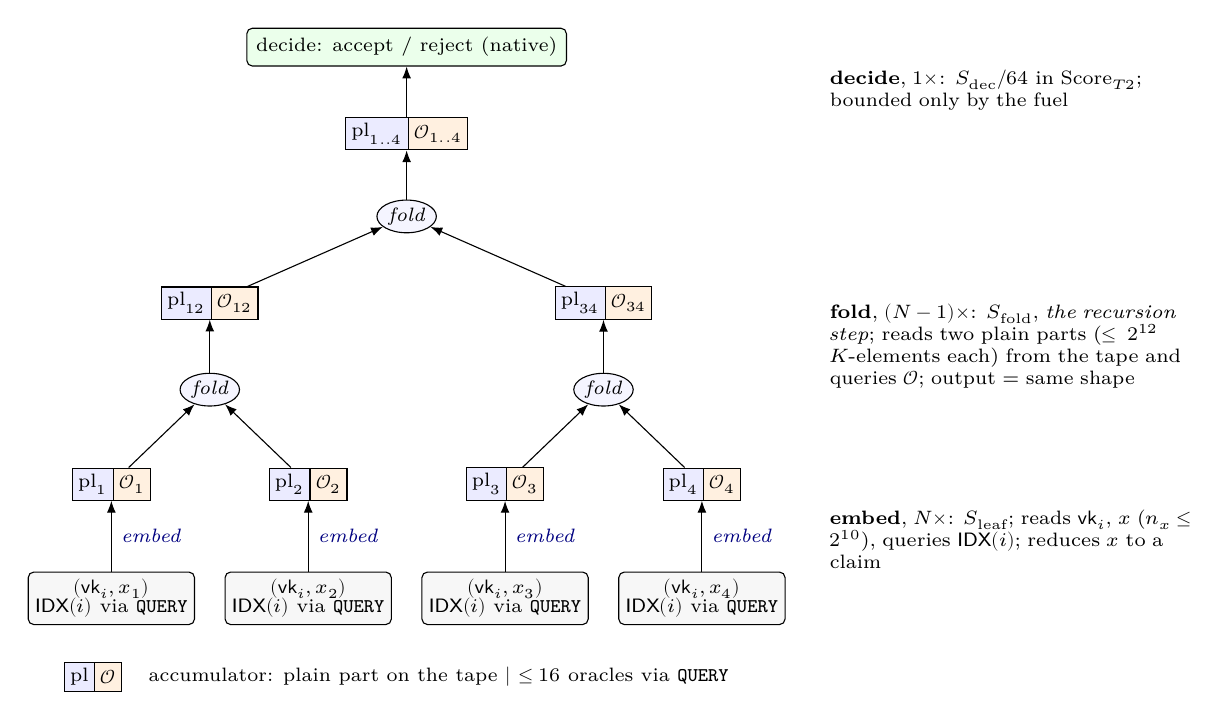
\begin{tikzpicture}[
  every node/.style={font=\small},
  leaf/.style={draw,rounded corners=2pt,fill=black!3,inner sep=2.5pt,align=center,font=\scriptsize},
  acc/.style={draw,rectangle split,rectangle split parts=2,rectangle split horizontal,
              inner sep=2pt,font=\scriptsize,rectangle split part fill={blue!8,orange!12}},
  fold/.style={draw,ellipse,inner sep=1pt,fill=blue!4,font=\scriptsize\itshape},
  cost/.style={font=\scriptsize,align=left,anchor=west,text width=4.6cm},
  arr/.style={-{Latex[length=1.5mm]}},
  qry/.style={densely dashed,-{Latex[length=1.2mm]},black!50}]
\foreach \j/\x in {1/0,2/2.5,3/5.0,4/7.5} {
  \node[leaf] (r\j) at (\x,0) {$(\vk_i,x_{\j})$\\[-1pt]$\idx(i)$ via \texttt{QUERY}};
  \node[acc] (a\j) at (\x,1.45) {$\mathrm{pl}_{\j}$\nodepart{two}$\mathcal O_{\j}$};
  \draw[arr] (r\j) -- node[right,font=\scriptsize\itshape,text=blue!50!black]{embed} (a\j);
}
\node[fold] (f12) at (1.25,2.65) {fold};
\node[fold] (f34) at (6.25,2.65) {fold};
\foreach \a/\f in {a1/f12,a2/f12,a3/f34,a4/f34} { \draw[arr] (\a) -- (\f); }
\node[acc] (b1) at (1.25,3.75) {$\mathrm{pl}_{12}$\nodepart{two}$\mathcal O_{12}$};
\node[acc] (b2) at (6.25,3.75) {$\mathrm{pl}_{34}$\nodepart{two}$\mathcal O_{34}$};
\draw[arr] (f12) -- (b1); \draw[arr] (f34) -- (b2);
\node[fold] (f) at (3.75,4.85) {fold};
\draw[arr] (b1) -- (f); \draw[arr] (b2) -- (f);
\node[acc] (c) at (3.75,5.9) {$\mathrm{pl}_{1..4}$\nodepart{two}$\mathcal O_{1..4}$};
\draw[arr] (f) -- (c);
\node[draw,rounded corners=2pt,fill=green!8,font=\scriptsize] (d) at (3.75,7.0) {decide: accept / reject (native)};
\draw[arr] (c) -- (d);
% cost column
\node[cost] at (9.0,0.75) {\textbf{embed}, $N\times$: $S_{\mathrm{leaf}}$; reads $\vk_i$, $x$
  ($n_x\le2^{10}$), queries $\idx(i)$; reduces $x$ to a claim};
\node[cost] at (9.0,3.2) {\textbf{fold}, $(N-1)\times$: $S_{\mathrm{fold}}$, \emph{the recursion
  step}; reads two plain parts ($\le2^{12}$ $K$-elements each) from the tape and queries
  $\mathcal O$; output = same shape};
\node[cost] at (9.0,6.45) {\textbf{decide}, $1\times$: $S_{\mathrm{dec}}/64$ in
  $\mathrm{Score}_{T2}$; bounded only by the fuel};
% legend
\node[acc,anchor=west] (lg) at (-0.6,-1.0) {pl\nodepart{two}$\mathcal O$};
\node[font=\scriptsize,anchor=west,align=left] at (0.35,-1.0) {accumulator: plain part on the tape $|$ $\le16$ oracles via \texttt{QUERY}};
\end{tikzpicture}
\caption{Where recursion pays. A 2-to-1 tree for $N=4$. Each accumulator has the fixed class shape:
a plain part on the tape and at most 16 committed oracles. Each arrow is a reduction with a one-step
Lean theorem (L1). The whole tree is covered by the organiser's \lean{tree\_secure} (L2, IT model).
The deployed system, where each fold verifier is compiled with a hash and proved inside the next
node's proof, rests on the named assumption \lean{RecursionHeuristic}
(\cref{subsec:rec-cannot}).}
\label{fig:rec-tree}
\end{figure}

%-----------------------------------------------------------------------------------------------
\subsection{What cannot be a Lean theorem}\label{subsec:rec-cannot}

The deployed system compiles each node's fold verifier with a hash $H$ (BCS and Fiat--Shamir) and
proves \enquote{the fold verifier accepted} inside the next node's proof. The proved relation
therefore queries $H$. Three results, summarised in \cref{subsec:bg-recursion}, bound what can be
said about that system.
\begin{enumerate}[nosep]
\item Succinct arguments for relations that themselves query the random oracle (relativized
  arguments) do not exist in the ROM, even interactive ones with computational soundness
  \cite{BCG24-RelROM}. A ROM proof of recursive soundness is therefore ruled out, not merely missing.
\item After the oracle is instantiated by a concrete hash, standard-model PCD theorems assume an
  extractor for the instantiated scheme, and they cover only constant depth: an extractor of size
  $|\tilde\Prv|^c$ per layer costs $|\tilde\Prv|^{c^d}$ at depth $d$ \cite[Rmk.~5.3]{BCMS20}. A
  2-to-1 tree has depth $\log_2N=\omega(1)$.
\item The only depth-free concrete bound \cite{CGSY24} needs a straight-line extractor for a
  relativized argument. For hash-based systems that is available only in a non-succinct idealisation,
  so it is heuristic evidence.
\end{enumerate}
leanerVM records the same gap as its open problem T6 (\enquote{recursive CTE}). It keeps the
end-to-end theorem as a target schema and forbids a global bridging axiom.\footnote{\repo{leanerVM@8aaf8a0}, \path{README.md:35-38},
\path{docs/architecture.md:297-350}, \path{AGENTS.md:81-83}.} The competition follows that policy.

\begin{assumption}{RecursionHeuristic}{Recursive deployment (named, never a Lean hypothesis of a scored theorem)}
Replacing the random oracle by the deployed hash inside the recursion circuit preserves straight-line
extraction of the accumulation scheme, with extractor time $t_E$. Under this assumption the advertised
security of a tree of $N$ nodes is $\kappa_{\mathrm{ARG}}(\lambda,q,s+O(N\cdot t_E))$, in the form
of \cite{CGSY24}. In the trusted repository this is prose plus an \emph{uninhabited} structure in
leanerVM's target-schema style:
\begin{leancode}
structure RecursionHeuristic (A : Accumulation k) (H : HashFn) : Prop where
  straightline_extractable : ...   -- prose in AUDIT.md; no instance
-- target schema; never proved, never a hypothesis of a scored theorem:
-- theorem recursive_sound (hA : A.Secure) (h : RecursionHeuristic A H)
--     (c : CompilerCorrect …) : …
\end{leancode}
\end{assumption}

Two more deployment facts are stated next to the assumption and are not part of any theorem.
\begin{itemize}[nosep]
\item \emph{Statement binding.} The R1CS is generated from programs, which is the precondition of
  \cite{Fen26-GenR1CS}; the harness's transcript prefix answers it by absorbing
  $\mathrm{MTroot}(\idx(i))$, $\vk_i$ and $x$ before the first challenge
  (\cref{subsec:sec-fs}). The recursion circuit also contains the Fiat--Shamir hash, the
  precondition of \cite{KRS25}; that attack is not answered by binding and is part of
  \lean{RecursionHeuristic}. For a fold node this means the two input plain parts and the roots of
  their accumulator oracles.
\item \emph{Extractor time.} The bound above is meaningful only if $t_E$ is polynomial. At L1 it is
  unconstrained, so the L2 efficient-extraction track is a precondition of the advertised bound.
\end{itemize}

%-----------------------------------------------------------------------------------------------
\subsection{Bounded-depth schemes and declared depth}\label{subsec:rec-depth}

Accumulation from linear codes without homomorphism \cite{BMNW24} checks linearity by spot-checks.
The new accumulator is then only guaranteed to be $\delta$-close to the claimed combination, and
every extraction step loses $\delta$. Soundness holds for a decider family
$\mathsf{D}_0\subseteq\dots\subseteq\mathsf{D}_d$, where $\mathsf{D}_s$ accepts words that are
$s\delta$-close to the code. Once $d\delta$ exceeds the unique-decoding radius there is a concrete
attack, not a gap in the proof. Arc and WARP remove the depth bound for RS and for general linear
codes respectively \cite{BMNW25-Arc,BCFW25-WARP}. The Lean shape of a bounded-depth scheme is
level-indexed: a relation $\Racc^{(s)}$ for each level $s\le d_{\max}$, a fold from
$\mathsf{pair}(\Racc^{(s)})$ to $\Racc^{(s+1)}$, and a decider per level.

\begin{decision}{REC-3}{Depth-uniform in the MVP; depth always declared and enforced}
The MVP certificate is depth-uniform (\cref{def:rec-acc}). The level-indexed generalisation is a
documented L2 extension. Every T2 record declares $d_{\max}$, and the harness and deployment
documentation enforce $d\le d_{\max}$. This applies even to depth-uniform schemes, because
\lean{tree\_secure} and the advertised bound are stated for $d\le d_{\max}$. \emph{Rationale:}
bounded-depth attacks are real, and arity bounds do not bound depth. leanVM's
\code{MAX\_RECURSIONS}$=16$ bounds the number of children per node, and leanerVM found no decreasing
depth measure in leanVM's aggregation.\footnote{\repo{leanerVM@8aaf8a0},
\path{docs/leanvm-target.md:90-94}; \repo{leanVM@a386121f},
\path{crates/rec\_aggregation/src/aggregation.rs:78}.} [D1 §4.2, §4.4; R7 §4.2]
\end{decision}

%-----------------------------------------------------------------------------------------------
\subsection{Full recursion (T3) is future work}\label{subsec:rec-t3}

The brief's \enquote{ambitious variant} arithmetises the verifier and measures a 2-to-1 step: the
fold verifier itself becomes an R1CS instance, and the step proves $\Vrf(\pi_1)\wedge\Vrf(\pi_2)$.
We schedule this as track T3, for three reasons.
\begin{enumerate}[nosep]
\item \emph{A trusted arithmetiser.} T3 needs an RV64IM+Zbc$\to$R1CS compiler whose correctness is
  part of the trusted base. That is a circuit-to-ISA correctness project of SP1/OpenVM scale. None
  exists for the contract's machine model.
\item \emph{Wall time.} A 2-to-1 wall-clock time depends on the machine and the prover
  implementation, and it is not reproducible. It can be a Yukon-style throughput board outside the
  Lean contract.
\item \emph{The fixed point does not close.} At $r$ R1CS constraints per RISC-V cycle, a verifier of
  $C$ cycles has an $r\cdot C$-constraint circuit. CPU-style arithmetisations need $r\approx30$--$100$
  (a judgement). \Cref{tab:rec-selfrec} applies this to the binary-field trajectory of
  \cref{sec:benchmark}. A self-recursive fixed point inside the $2^{24}$ class needs
  $C\le2^{24}/r$, i.e.\ $1.7$--$5.6\times10^5$ cycles. The best modelled design (B3) is 9--29 times
  above that.
\end{enumerate}

\begin{table}[t]
\centering\small
\begin{tabular}{@{}lrrr@{}}
\toprule
Verifier (cycles at the $2^{24}$ class) & $C$ & $\log_2(rC)$, $r=30$ & $r=100$ \\
\midrule
B1: Spartan + binary WHIR-JB, $\rho=1/2$ & $6.2\times10^6$ & 27.5 & 29.2 \\
B3: B1 at $\rho=1/16$ & $4.8\times10^6$ & 27.1 & 28.8 \\
B5: B1, unique-decoding regime & $1.1\times10^7$ & 28.3 & 30.0 \\
leanVM 2$\to$1 step, naive port to RV64IM+Zbc & $\approx3\times10^7$ & 29.8 & 31.5 \\
\midrule
fixed point inside $2^{24}$ requires & $\le2^{24}/r$ & 24 & 24 \\
\bottomrule
\end{tabular}
\caption{Self-recursion arithmetic over $K/E$ [D3 §6.2, reading 6; D2 §7.4]. Cycle counts are model
estimates ($\pm2\times$). leanVM itself runs a 2$\to$1 step in 0.56--0.69\,M steps of its
field-native ISA \cite{leanVM}; a leanISA step is worth 1--139 weighted RV64IM+Zbc cost units depending on the
opcode (an $E$ multiplication is 103 instructions, 139 units under v0.2's display weights with \texttt{clmul} at 4), so the two numbers are not comparable.}
\label{tab:rec-selfrec}
\end{table}

Closing the gap needs field and hash support in the ISA, which is the field-syscall board T1-F with an
\texttt{EMUL} syscall priced from a binary-field zkVM, or classes up to $2^{28}$
(\cref{sec:cost}). The contract's class ladder is nested and can be extended without changing theorem
shapes. In the meantime, T2's fold-verifier cycle count on the contract machine is the competition's
proxy for recursion cost: it is what a fixed zkVM would arithmetise. The L4 statement exists only as
the target schema \lean{recursive\_sound} above.

\begin{takeaway}[Summary]
The brief's batcher becomes an accumulation scheme: embed, fold and decide, each with the base
track's certificate, an accumulator shape fixed by type, and output agreement on the machine. Lean
certifies one step (L1) and, once the frame rule exists, the tree (L2), both in the IT model. Security
of the compiled recursive system is the named \lean{RecursionHeuristic}, with declared depth. The
fold verifier's cycles are the recursion cost that T2 scores, against the \lean{fullRecAcc} baseline
that equals T1.
\end{takeaway}

% Provenance: copied from the design workspace CambridgePQ/recursion.fast, `report/sections/10-cost.tex`, on 2026-10-19. Read-only copy; the source is authoritative.
% 10-cost -- written by W3 (revised for cost model v0.3)
\section{Cost function and incentives}\label{sec:cost}

The score must track what recursion pays, and it must be a kernel-checked theorem, not a
measurement. Earlier golf competitions priced every RISC-V instruction alike, and agents optimised
that model rather than the problem. This section gives cost model v0.3 (DESIGN §15), which replaces
the flat per-instruction weights of v0.2. It proceeds in order:
\begin{itemize}[nosep]
\item the evidence that a flat per-instruction model is overfit;
\item the two machines the competition prices: a zkVM for the recursion step and a multicore CPU for
  native verification;
\item the one proved object: an 18-counter cost vector over accepting runs;
\item the two boards built on it: the recursion board, a geometric mean over four calibrated zkVM
  profiles, and the latency board, a deterministic timing model with fork-join harts;
\item the parts of v0.2 that carry over: the accepting-run bound, honest preprocessing, caps, the
  Fiat--Shamir surcharge and the blow-up factor;
\item what it costs to implement, and what remains unrealistic.
\end{itemize}
Fields are $K=\mathrm{GF}(2^{64})$ and $E=K[y]/(y^3+y+1)=\mathrm{GF}(2^{192})$
(\cref{subsec:bg-binary}). The machine is RV64IM plus the carry-less-multiply extension Zbc
(\cref{subsec:proto-machine}). Kernel costs come from one emulator trace priced under nine models at once.
Trajectory numbers are model estimates, accurate to about a factor of 2.

%-----------------------------------------------------------------------------------------------
\subsection{Diagnosis: how a flat per-instruction model is overfit}\label{subsec:cost-diagnosis}

\paragraph{What the golf competitions produced.} sig.golf scores one cycle per instruction, four per
multiplication, and treats code as free up to 1\,MiB. Its accepted verify image has 145{,}952
instructions.
\begin{itemize}[nosep]
\item 98{,}134 of them are NOPs (\textbf{67\%}): padding that keeps code at fixed 256-word pitches so
  that table-driven dispatch can \texttt{jalr} into slots.
\item Of the 47{,}818 remaining words, \textbf{59\% are stores and 28\% are \texttt{jal}s}. The code is
  straight-line and table-driven: it stages constants into memory and hops between slots. It contains
  867 loads, 345 ALU operations and 279 branches in all.
\end{itemize}
That code is optimal only where a store and a jump each cost 1 and code size, instruction cache and
paging cost nothing. On RISC~Zero, 584\,KB of straight-line code would page in at about 1{,}130 cycles
per KiB, i.e.\ about 660k cycles against a claimed 11{,}687.

ots.golf counts \textbf{one hash compression as one instruction}. A full-length acceptance is 192
compressions plus 149 instructions, so hashing is 56\% of the score. At a software BLAKE2s cost of
1{,}560--2{,}770 cycles it would be more than 99.9\% of the time. One ots.golf track's record moved from
49{,}335 to 1{,}088 within a week: the agents converged on the model, not on the problem.

\paragraph{Mispricings on this competition's kernels.} One trace of each kernel was priced under nine
models:
\begin{itemize}[nosep]
\item \texttt{uni}, the v0.2 weights;
\item five zkVM weightings: \texttt{zisk}, \texttt{sp1} (no Zbc chip, as SP1 is today), \texttt{sp1z}
  (with a hypothetical Zbc chip), \texttt{r0} (RISC~Zero) and \texttt{jolt};
\item a generic memory-priced zkVM, \texttt{zkmem};
\item an in-order dual-issue scoreboard with caches (\texttt{inord}), using SiFive-7 and SpacemiT-X60
  latencies from GCC's scheduler models;
\item an idealised 4-wide out-of-order dataflow model (\texttt{ooo}).
\end{itemize}
The v0.2 model gets five things wrong:
\begin{itemize}[nosep]
\item \emph{Multiplication.} MUL $=$ CLMUL $=4$ is about 3 times the area ratio of real zkVMs (ZisK
  1.29, SP1 1.38). Field kernels cost 0.7--0.8 times v0.2 under every Zbc-equipped zkVM profile, and
  0.5 times on an in-order core.
\item \emph{Memory and paging.} Loads cost the same as ALU operations, and first touches and paging
  cost nothing. A random 8-byte gather over 4\,MiB costs 13 under \texttt{uni} and 87 on the in-order
  core. On that core the trivial baseline at $2^{20}$ costs 3.2 times its v0.2 count, 65\% of it DRAM
  stalls. One MiB of proof read once costs about 1.16M cycles on RISC~Zero, 9 times the v0.2 byte
  charge.
\item \emph{Code size.} Free code means unrolling wins under \texttt{uni} (1.66 times cheaper) and loses
  under every realistic model: 6 times dearer in-order, 17 times out-of-order, 1.4 times on RISC~Zero.
\item \emph{Hashing.} The virtual Merkle level at 43 is 2.5--5 times below zkVM precompile prices and 37
  times below a native core.
\item \emph{No instruction-level parallelism.} Independent multiplication chains run 1.5--1.9 times faster
  on a real out-of-order core, and no per-instruction count sees it.
\end{itemize}
On field kernels every realistic model is a near-uniform 0.5--0.8 of v0.2. On memory-, control- and
code-bound kernels the ratios are 1.2--8. The flat model's \emph{relative} error across kernel
classes therefore spans about \textbf{15 times}. Seven of thirteen paired kernels change winner under
at least one model (\cref{tab:cost-flips}). Three of those flips are robust to the pipeline parameters:
branchless code under \texttt{ooo}, code size, and tables without Zbc.

\begin{table}[t]
\centering\footnotesize
\setlength{\tabcolsep}{3.5pt}
\begin{tabular}{@{}>{\raggedright\arraybackslash}p{4.6cm}rrrrrrrr@{}}
\toprule
Pair (cost of A $/$ cost of B; $>1$: B wins) & uni & zisk & r0 & jolt & sp1 & sp1z & inord & ooo \\
\midrule
$E$ mult.: Karatsuba / schoolbook & 0.89 & 1.00 & 1.03 & 1.00 & 0.68 & 0.99 & 0.88 & 1.00 \\
$K$ inverse: Fermat / Itoh--Tsujii & 1.71 & 1.70 & 1.50 & 1.69 & 1.76 & 1.70 & 1.49 & \textbf{0.78} \\
$K$ square: clmul / 16\,KiB tables & 0.56 & 0.51 & 0.55 & 0.45 & \textbf{6.14} & 0.49 & 0.54 & 0.79 \\
dispatch: jump table / if-chain & 0.67 & 0.63 & 0.74 & 0.77 & 0.68 & 0.68 & \textbf{1.11} & \textbf{1.18} \\
branchy / branchless (random bit) & 0.66 & 0.63 & 0.77 & 0.69 & 0.64 & 0.64 & 0.86 & \textbf{2.56} \\
staging: unrolled (24\,KiB code) / loop & 0.60 & 0.53 & \textbf{1.37} & 0.60 & 0.62 & 0.62 & \textbf{5.88} & \textbf{16.7} \\
loads: random 4\,MiB / sequential & 3.25 & 3.58 & 6.40 & 3.25 & 3.42 & 3.42 & 21.6 & 11.7 \\
\bottomrule
\end{tabular}
\caption{Paired kernels under nine cost models (selection; \texttt{zkmem} omitted). Bold entries change
the winner relative to \texttt{uni}; the last row keeps its winner but changes its magnitude 7-fold
[D4 §1.2; probe \texttt{d4-probes}]. The jump-table flip is sensitive to the pipeline parameters; the
branchless, code-size and no-Zbc flips hold under every setting.}
\label{tab:cost-flips}
\end{table}

\paragraph{Architecture or engineering?} Re-running the trajectory model under the nine models
(\cref{subsec:bench-trajectory}, \cref{tab:bench-models}) shows that v0.2 ranks \emph{architectures}
tolerably: the top three designs are stable. It mis-ranks \emph{engineering} and mis-states
\emph{where the cost is} (hashing on native cores, bytes on RISC~Zero). The fix is cheap for the zkVM
board, by re-weighting, and needs a timing model for the CPU board.

%-----------------------------------------------------------------------------------------------
\subsection{Candidate cost models}\label{subsec:cost-candidates}

\Cref{tab:cost-candidates} lists the candidates. Four requirements decide between them.
\begin{itemize}[nosep]
\item \emph{Dimension.} The score must be monotone in what users pay.
\item \emph{Ungameability.} No prover-side or benchmark-side choice may move it.
\item \emph{Realism.} It must resist the overfitting described above.
\item \emph{Provability.} It must follow from a theorem whose proof technique exists.
\end{itemize}

\begingroup\small
\renewcommand{\arraystretch}{1.12}
\begin{longtable}{@{}>{\raggedright\arraybackslash}p{0.27\textwidth}>{\raggedright\arraybackslash}p{0.22\textwidth}>{\raggedright\arraybackslash}p{0.45\textwidth}@{}}
\caption{Candidate cost models and verdicts.}\label{tab:cost-candidates}\\
\toprule
Candidate & Form & Verdict \\
\midrule
\endfirsthead
\toprule
Candidate & Form & Verdict \\
\midrule
\endhead
Brief: performance $\div$ size & cycles $/$ bytes & rejected: dimensionally inverted, and any size term rewards obfuscation. Replaced by a hard 1\,MiB cap \\
sig.golf product & bytes $\times$ cycles & rejected for the primary board: fixes an arbitrary exchange rate. Kept as the shape of the proof-size board \\
Flat per-instruction weights (v0.2) & $(1;\ \mathtt{MUL}=\mathtt{CLMUL}=4)$ & superseded: overfit, with a relative error spanning about 15 times across kernel classes (\cref{subsec:cost-diagnosis}). Kept as an unscored display column \\
One calibrated zkVM profile & $w_P\cdot c$ & rejected alone: invites overfitting to one zkVM, whose costs also change between releases \\
\textbf{Four calibrated profiles, geometric mean} & $\bigl(\prod_P\prod_kS_{P,k}\bigr)^{1/12}$ & \textbf{adopted} for the recursion board (\cref{subsec:cost-zk}) \\
Minimum or maximum over profiles & $\min_P$, $\max_P$ & $\min$ rewards overfitting. $\max$ (minimax) is defensible but brittle to one mis-calibrated profile \\
\textbf{Deterministic in-order timing model + fork-join harts} & $T_{16}=W/16+S$ & \textbf{adopted} for the latency board (\cref{subsec:cost-lat}) \\
Cache and DRAM model in the proof & first-touch line sets & deferred: provable only for statically known address ranges; first-touch \emph{counts} are adopted instead \\
Wall time on reference hardware & seconds & calibration and display only: noise of $\pm2$--$5\%$ against sub-percent record margins, not a theorem, and it would put candidate code on the score's trust path \\
Wall time of a 2$\to$1 recursion step & seconds & deferred: needs a trusted arithmetiser (T3, \cref{subsec:rec-t3}) \\
Measured median on hash chains & -- & rejected as a score: gameable by special-casing \\
All-runs or honest-runs bound & see \cref{tab:cost-clauses} & superseded by the accepting-run bound \\
\bottomrule
\end{longtable}
\endgroup

\begin{decision}{COST-1}{Two machines, two boards, one proved vector}
The \emph{recursion board} (machine M-zk) is primary. It prices the prover cost of the verifier's
trace in a zkVM, as a geometric mean over four calibrated zkVM profiles. The \emph{latency board}
(machine M-cpu) is a separate leaderboard, scored from season~1. It prices native multicore
verification, which matters for the decider and for node verification, with a deterministic
pipeline-and-harts model. Both are computed from proved bounds. Wall time is calibration and display
only, and the v0.2 flat weights are a display column. \emph{Rationale:} the two machines reward
different code (branches, tables, unrolling). A combined score would let one hide the other.
\emph{Answers:} user input U3 (flat per-instruction costs are overfit; parallelism is not accounted for). [DESIGN
§15.1; D4-1--D4-3]
\end{decision}

%-----------------------------------------------------------------------------------------------
\subsection{The proved object: an 18-counter vector over accepting runs}\label{subsec:cost-vector}

The cost theorem bounds a vector of monotone counters, not a scalar:
\begin{multline*}
  c=(n_{\mathrm{add}},n_{\mathrm{logic}},n_{\mathrm{shift}},n_{\mathrm{mul}},n_{\mathrm{div}},
     n_{\mathrm{clmul}},n_{\mathrm{ld}},n_{\mathrm{ldsub}},n_{\mathrm{st}},n_{\mathrm{stsub}},
     n_{\mathrm{br}},n_{\mathrm{jmp}},n_{\mathrm{sys}},\\
     m_{\mathrm{words}},m_{\mathrm{pages}},q^{\mathrm{count}},q^{\mathrm{lev}},q^{\mathrm{bytes}}).
\end{multline*}
\begin{itemize}[nosep]
\item Instruction counters separate addition, logic, shifts, multiplication, division and Zbc, and
  split loads and stores into doubleword and sub-doubleword accesses. Branches and jumps are counted
  apart.
\item $m_{\mathrm{words}}$ and $m_{\mathrm{pages}}$ count \emph{first-touched} doublewords and 1\,KiB
  pages. They cover code and data, and \texttt{QUERY} destinations count like stores. In the Lean
  machine, \lean{execute} threads three \lean{Finset}s (doublewords, pages, written pages), and the
  counters are their cardinalities at the end of the run (\lean{Acct.vec}; a written page counts twice).
\item $q^{\mathrm{count}}$, $q^{\mathrm{lev}}=\sum\mathsf{depth}_j$ and
  $q^{\mathrm{bytes}}=\sum\mathsf{leafbytes}_j$ are summed over the \texttt{QUERY}s of a run.
\end{itemize}
Every profile is a non-negative linear function of $c$. A weighted sum of componentwise maxima bounds
the maximum of the weighted sums: $\sum_iw_i\max_{\mathrm{run}}n_i\ge\max_{\mathrm{run}}\sum_iw_in_i$.
So \emph{one} certificate is a valid bound under every profile and under every later re-weighting.
Proving it uses the same loop invariants as before, carried with a tuple. For the first-touch
counters the library has per-touch cardinality lemmas; a footprint combinator for loops that write
$[\mathit{base},\mathit{base}+8n)$ is planned (L-10), and the baseline wrote its own invariant.
The clause is the contract's (\cref{subsec:app-cost} has the whole file):

\begin{leancode}[label={\footnotesize Contract/Cost.lean}]
def Protocol.AcceptingCostAtMost {sz : Sizes} (P : Protocol sz) (img : Image) (c : CostVec) : Prop :=
  ∀ (i : Index sz) x (tr : FullTranscript P.shape) v s, run img (P.tape i x tr) (P.oracles i tr) =
      some (v, s) → v ≤ c
\end{leancode}
Here \lean{run} returns \lean{some} exactly on acceptance, with the 18 counters and the final state;
the tape holds the sizes, the honest \lean{VK i}, $x$ and the challenges of \lean{tr}, and the
oracles are the honest \lean{IDX i} followed by the raw messages of \lean{tr}. So the quantifier
ranges over every index of the size, every public input, every raw oracle content and every
challenge vector, and \lean{≤} is componentwise.

\phantomsection\label{subsec:cost-u2}%
\paragraph{Fuel.} Each hart runs for at most $F=2^{36}\approx6.9\times10^{10}$ steps, and fuel
exhaustion is a rejection. No separate termination theorem is needed: $\mathsf{Agrees}$ already forces
every spec-accepted transcript, including every honest one, to be accepted within fuel. $F$ is a
contract constant that counts executed instructions (steps), not weighted cost. It is per hart: a
child runs with its parent's remaining fuel, and the parent is not charged for the child's steps, so
a run with harts can take up to $(\#\mathrm{spawns}+1)\cdot2^{36}$ steps (A6-F1, row H12). The certified baseline's
accepting runs at $2^{24}$ take $3.09\times10^9$ steps, 4.5\% of $F$ (\cref{sec:baseline}); a succinct
design takes about $10^{6}$--$10^{7}$ steps, so $F$ leaves a margin of $10^4$ or more.

\paragraph{Why accepting runs, and exploits attempted.} \Cref{subsec:obj-what} gives the argument: only
accepting executions are ever arithmetised, the clause covers every honest run and every accepting
run on an adversarial transcript, and a verifier cannot make acceptance cheap selectively without
breaking soundness. \Cref{tab:cost-u2-exploits} lists the attempts made in design note D3; none
gains anything over the all-runs clause, and re-weighting does not touch the argument.

\begingroup\small
\renewcommand{\arraystretch}{1.1}
\begin{longtable}{@{}p{0.03\textwidth}>{\raggedright\arraybackslash}p{0.36\textwidth}>{\raggedright\arraybackslash}p{0.55\textwidth}@{}}
\caption{Attempted exploits of the accepting-run clause [D3 §4.3].}\label{tab:cost-u2-exploits}\\
\toprule
\# & Attempt & Outcome \\
\midrule
\endfirsthead
\toprule
\# & Attempt & Outcome \\
\midrule
\endhead
1 & Quick accept for honest-looking proofs, long check otherwise & every accepting run is bounded; a sound quick path is just a cheaper verifier \\
2 & Optional cheap \enquote{easy mode} protocol chosen by the prover & the maximum over both modes is scored \\
3 & Move work into pre-checks that reject & the accepting path executes every pre-check that passes \\
4 & Loop trip counts read from the proof & bounded on accepting runs by the consistency check; rejecting runs stop at $F$ \\
5 & Data-dependent \texttt{QUERY} counts & $q^{\mathrm{count}}\le Q_k$ on accepting runs \\
6 & Vacuity on unsatisfiable indices & harmless: unprovable statements are never verified, and honest runs accept on every satisfiable index \\
7 & Make accepting runs on false statements expensive & inside the bound; see 1 \\
8 & Trap to escape the bound on a long path & a fault is a reject; acceptance requires \texttt{HALT} with $a_0=1$ \\
9 & T2: cheap output accumulator, defer everything & output shape fixed and pinned by $\mathsf{Agrees}$; deferral is paid at $S_{\mathrm{dec}}/64$; the decider is bounded only by the fuel \\
10 & Grind the demonstration run & demonstrations are unscored; the badge checks measured $\le$ claimed \\
\bottomrule
\end{longtable}
\endgroup

\paragraph{Pitfalls.} (1) \emph{Denial of service.} A verifier may spend up to $F$ steps rejecting,
about 10--20\,s natively, and up to $(\#\mathrm{spawns}+1)\cdot F$ with harts (H12). The planned
mitigations, not in the v0.3 contract, are an optional displayed all-runs badge and, for T2
deciders, a required bound $C^{\mathrm{all}}_{\mathrm{dec}}\le8\,C_{\mathrm{dec}}$ (R-3).
(2) \emph{Proof burden.} After the honest-preprocessing fix, the
accepting and all-runs clauses differ by 5--15\% of the machine-level proof. The main saving is that no
termination theorem is proved [A3 n2]. (3) \emph{Hygiene.} There is one componentwise bound on one
vector, and every score is a Lean function of it (\cref{subsec:cost-zk}).

\begin{table}[t]
\centering\small
\begin{tabularx}{\linewidth}{@{}>{\raggedright\arraybackslash}p{2.6cm}>{\raggedright\arraybackslash}X>{\raggedright\arraybackslash}p{3.4cm}>{\raggedright\arraybackslash}X@{}}
\toprule
Clause & Quantifies over & Precedent & Deployment meaning \\
\midrule
All runs & every input and oracle & ots.golf RISC-V \lean{cycles} & cost bound plus DoS bound; ranking arguments on every data-driven loop \\
\textbf{Accepting runs (adopted)} & every input on which the machine accepts & ots.golf hinted track (every prover-chosen view, accepting executions) & exactly the recursion cost; DoS bounded only by $F$ per hart \\
Honest runs & honest transcripts under every fixed oracle & sig.golf \lean{verificationCycles} & too weak: an accepted dishonest transcript may run longer \\
\bottomrule
\end{tabularx}
\caption{Cost clauses and precedents (\cref{sec:prior}).}
\label{tab:cost-clauses}
\end{table}

\paragraph{Honest preprocessing.} The first design quantified the cost clause over every oracle,
including oracle~0, the index. Under that quantifier the baseline's claimed bound is \emph{false}
[A3-C2]. The baseline reads row and nonzero counts from $\vk$ and $\idx$.
\begin{itemize}[nosep]
\item A huge count makes a loop walk memory until a load faults. Under the all-runs clause that alone
  costs about $10^{10}$ steps in every class.
\item The accepting-run clause does not rescue it. Filling oracle~0 to its admitted length $2^{k+10}$
  with zero-valued entries makes every row hold trivially. The run then \emph{accepts} after about
  $20\cdot2^{k+9}$ steps, about 22 times the claimed $C_k$.
\end{itemize}
The fix loses nothing. $\vk_i$ and $\idx(i)$ are outputs of the deterministic, computable Lean
indexer. The harness computes them and binds $\mathrm{MTroot}(\idx(i))$ and $\vk_i$ into the
Fiat--Shamir prefix, and $\mathsf{Secure}$ and $\mathsf{Agrees}$ are already stated for them. Every
machine clause therefore quantifies over honest preprocessing ($\forall i$ of class shape). The prover
and environment inputs stay adversarial: $x$, every raw oracle content and every challenge. In
deployment this is the standard holographic assumption that the verifier holds the honest key. As a
side effect, trip counts come from $k$ and $\vk_i$, never from prover data, so cost proofs need no
ranking arguments.

%-----------------------------------------------------------------------------------------------
\subsection{The recursion board: four calibrated zkVM profiles}\label{subsec:cost-zk}

\paragraph{Profiles.} Each profile $P$ is a weight vector $w_P$ on the instruction and memory
counters, a hash price $P_{H,P}$ per 64-byte compression, and a byte charge $\lambda_P$. The weights were
normalised from primary cost tables:
\begin{itemize}[nosep]
\item ZisK: area $\times$ operation from \texttt{zisk\_ops\_costs.rs} and the memory state-machine
  columns;
\item SP1 Hypercube: trace area per event from \texttt{rv64im\_costs.json}, with fetch and decode charged
  per executed instruction and a hypothetical Zbc chip priced like MUL;
\item RISC~Zero: one cycle per instruction, 2 for bitwise and division, 1{,}130 cycles per 1\,KiB page
  touched (the documented average of 1{,}094--5{,}130);
\item Jolt: lookup-uniform, with virtual division sequences and expensive sub-word stores.
\end{itemize}
\Cref{tab:cost-profiles} gives the weights.

\begin{table}[t]
\centering\footnotesize
\setlength{\tabcolsep}{4pt}
\begin{tabular}{@{}lrrrrr@{}}
\toprule
Counter & ZK-A ZisK & ZK-B SP1-H & ZK-C RISC~Zero & ZK-D Jolt & v0.2 (display) \\
\midrule
$n_{\mathrm{add}}$ (add[w], sub[w], addi[w], lui, auipc, fence) & 0.73 & 1.00 & 1 & 1 & 1 \\
$n_{\mathrm{logic}}$ (and, or, xor, slt, with imm.) & 1.00 & 1.10 & 2 & 1 & 1 \\
$n_{\mathrm{shift}}$ & 0.97 & 1.27 & 1 & 1 & 1 \\
$n_{\mathrm{mul}}$ & 1.29 & 1.38 & 1 & 1 & 4 \\
$n_{\mathrm{div}}$ & 1.29 & 2.64 & 2 & 8 & 4 \\
$n_{\mathrm{clmul}}$ & 0.97 & 1.38\,[J] & 1\,[J] & 1\,[J] & 4 \\
$n_{\mathrm{ld}}$ / $n_{\mathrm{st}}$ (doubleword) & 0.60 & 1.05 & 1 & 1 & 1 \\
$n_{\mathrm{ldsub}}$ / $n_{\mathrm{stsub}}$ (sub-doubleword) & 0.60 & 1.10 / 1.13 & 1 & 3 / 9 & 1 \\
$n_{\mathrm{br}}$ & 1.00 & 1.09 & 1 & 1 & 1 \\
$n_{\mathrm{jmp}}$ (jal, jalr) & 0.73 & 1.00 & 1 & 1 & 1 \\
$n_{\mathrm{sys}}$ (HALT, SPAWN, JOIN) & 1 & 1 & 1 & 1 & 1 \\
$m_{\mathrm{words}}$ (first-touched doublewords) & 0 & 0.12 & 0 & 0 & 0 \\
$m_{\mathrm{pages}}$ (first-touched 1\,KiB pages) & 0 & 0 & 1{,}130 & 0 & 0 \\
$P_{H,P}$ per compression (level: $+35$) & 72 & 174 & 100\,[J] & 200\,[J] & 8 \\
$\lambda_P$ per proof byte & 1/8 & 1/8 & 1/8 & 1/8 & 1/8 \\
\bottomrule
\end{tabular}
\caption{zkVM profiles of the recursion board [D4 §2a]. [J] marks a judgement. The three
non-ZisK Zbc entries assume a carry-less-multiply chip that SP1, RISC~Zero and Jolt do not have today.
The RISC~Zero and Jolt hash prices are guesses, to be replaced from published accelerator costs.}
\label{tab:cost-profiles}
\end{table}

The spread \emph{between} zkVMs on ALU-class operations is only 0.7--1.4 times. On memory footprint
(0 to 1{,}130 per KiB), sub-word stores (1 to 9), division (1.3 to 8) and hashes (72 to 200 per
compression, against 8 in v0.2) it is 10--100 times. These are exactly the counters v0.2 lacked.

\paragraph{\texttt{QUERY}: a virtual Merkle opening.} \texttt{QUERY} returns a whole declared leaf of
$\mathsf{leaf}_j$ $K$-elements of oracle $j$, which has length $\ell_j$. With
$\mathsf{depth}_j=\log_2(\ell_j/\mathsf{leaf}_j)$ (both powers of two) and
$b_j=\mathsf{leafbytes}_j=8\,\mathsf{leaf}_j$, a compiled verifier hashes the leaf, $\lceil b_j/64\rceil$
compressions, and one node per level. The exact price of one call under profile $P$ is therefore
\[
  \mathsf{depth}_j\cdot(P_{H,P}+35)+P_{H,P}\cdot\lceil b_j/64\rceil .
\]
The $+35$ is the measured non-hash cost of one level. The certificate does not carry
$\sum_i\lceil b_i/64\rceil$, so the contract charges the leaves of a run through the upper bound
\[
  \sum_i\Bigl\lceil\frac{b_i}{64}\Bigr\rceil\;\le\;\sum_i\Bigl(\frac{b_i}{64}+1\Bigr)
  \;=\;\frac{q^{\mathrm{bytes}}}{64}+q^{\mathrm{count}},
  \qquad\text{charged as } P_{H,P}\cdot\Bigl(\frac{q^{\mathrm{bytes}}}{64}+q^{\mathrm{count}}\Bigr),
\]
which uses only existing counters and over-charges by at most one compression per \texttt{QUERY}
(\lean{Profile.C}; the docstring gives the argument). Returning whole leaves is deliberate. With
single-element queries, a $2^4$-fold query would pay 16 paths. An amortised per-element price would be
gamed by declaring huge leaves and reading one element of each. A depth-0 round is a plain read,
priced by its leaf hash and its bytes. Every call is charged; caching is the verifier's own job.

\paragraph{The leaf-pricing hole closed in round~3 (A6-P1).} v0.2 charged the leaf as
$q^{\mathrm{bytes}}/8$, exactly the leaf hash at v0.2's $P_H=8$; v0.3 first rescaled $P_H$ per profile
for the levels and the absorption but left the leaf at that rate, 9--25 times below its hash cost.
Review A6 measured the consequences with the contract's own functions (\path{probes/a6-probes/Pricing.lean},
re-run in CI): moving a 1{,}024-word $\vk$ into the index oracle undid the A4-F6 fix, lowering the
$C+\mathit{FS}+\lceil\lambda B\rceil$ term by 7--45\%, and the charged score-optimal leaf was
$2^6$--$2^7$ against a true optimum of $2^4$. Under the corrected price the move costs exactly one
$P_{H,P}$ more than tape absorption (theorem \lean{vk\_in\_idx\_no\_gain}; RISC~Zero more, through
paging), the charged optimum is $\mathsf{leaf}=2^4$ in every profile, and a kernel-checked lemma gives
$\text{exact}\le\text{charged}\le\text{exact}+P_{H,P}$ for $\mathsf{leaf}\le2^{12}$ (row C25 has the
numbers). The latency board still charges the leaf one cycle per element (M-6).

\paragraph{Fiat--Shamir surcharge, per profile.} In the IT model challenges are free tape contents. A
compiled verifier absorbs the statement and every root, and squeezes every challenge. The contract
fixes the challenge menu: $E$-vectors and bounded indices, with no submitter-chosen types. That removes
the free \emph{derived} values a submitter type would let the harness compute, such as barycentric
weights, powers, inverses and $\mathrm{eq}$ tables [A1-M1]. What remains is priced statically from the
declared shapes:
\[
  FS_{P,k}=\mathrm{rounds}_k\,(2P_{H,P}+30)+n^{E}_k\,(0.75\,P_{H,P}+6)+4\,n^{\mathrm{idx}}_k
  +\Bigl\lceil\tfrac{(\mathsf{vkLen}+n_x)\cdot8}{64}\Bigr\rceil\,P_{H,P}.
\]
\begin{itemize}[nosep]
\item Per round: absorb a 32-byte root (one compression plus about 30 ALU operations) and squeeze one
  block.
\item Per $E$ element: 24 squeezed bytes, i.e.\ 0.75 compressions, plus loads. No reduction is needed,
  because every 24-byte string is an $E$ element.
\item Per index challenge: mask $b$ bits.
\item Per class: absorb the prefix $\vk_i\,\|\,x$, at most $256$ compressions at
  $\mathsf{vkLen}=n_x=2^{10}$. A4 found that v0.2 omitted this term [A4-F6].
\end{itemize}
At $P_H=8$ the first three terms reduce to v0.2's $46/12/4$.

\paragraph{Bytes and blow-up.} The byte count is
$B_k=\mathsf{tapeBytes}_k+q^{\mathrm{bytes}}_k+32\,q^{\mathrm{lev}}_k+32\cdot\#(\text{msg rounds})_k$.
It charges one digest per virtual level and one root per round, which closes the free-Merkle-cap
channel [A1-m3]. The charge $\lambda_P=1/8$ is a monotonicity device; small proofs are rewarded by the
proof-size board. RISC~Zero's paging now charges first-touched proof bytes through $m_{\mathrm{pages}}$,
about 1.1 cycles per byte. Rate is priced by
\[
  V_k=\sum_{j\ge1}\frac{\ell_j}{N_k+2^{k+4}}\quad(\idx\text{ excluded}),\qquad
  \text{factor }\max(1,V_k/16)^{1/4},\qquad V_k\le2^8 .
\]
Without it, every record would sit on the rate cap [A1-M4]. Threshold 16 makes SPARK at $\rho=1/2$
free. Exponent $1/4$ turns rate into a visible slope: exponent 0 puts the optimum at the cap and
exponents of $1/2$ or more force $\rho=1/2$.

\phantomsection\label{subsec:cost-score}%
\paragraph{The score.} For profile $P$ and class $k\in\{16,20,24\}$, with $c_k$ certified by
$\mathsf{AcceptingCostAtMost}(k,c_k)$:
\begin{align*}
  S_{P,k}&=\Bigl(w_P\cdot c_k+(P_{H,P}+35)\,q^{\mathrm{lev}}_k
           +P_{H,P}\bigl(q^{\mathrm{bytes}}_k/64+q^{\mathrm{count}}_k\bigr)+FS_{P,k}
           +\lceil\lambda_PB_k\rceil\Bigr)\cdot\max(1,V_k/16)^{1/4},\\
  \mathrm{Score}_{zk}&=\Bigl(\prod_{P\in\{A,B,C,D\}}\prod_{k}S_{P,k}\Bigr)^{1/12},\qquad
  \mathrm{Score}_{T2}\text{: the same with }S_{\mathrm{leaf}}+S_{\mathrm{fold}}+S_{\mathrm{dec}}/64 .
\end{align*}
Lower is better. Three properties make it hard to game.
\begin{itemize}[nosep]
\item \emph{Normalisation cancels.} Rankings under a geometric mean do not depend on per-profile
  normalisation constants, because those cancel in the ratio between two submissions.
\item \emph{Specialisation is visible and bounded.} Tanking one profile by a factor of 2 costs
  $2^{1/4}$, i.e.\ 19\%, overall, and the four per-profile scores are displayed.
\item \emph{The score is a theorem.} The scores are Lean functions of the certified data (\lean{scoreZk4}
  returns the fourth powers in $\mathbb Q$). The challenge renders the image bytes and every
  shape-derived input, and the certificate proves the claimed per-profile values. The external scorer
  only takes roots [A4-F2, F4].
\end{itemize}

\begin{decision}{COST-2}{Seasonal re-weighting without re-proof}
The profile family and its aggregation are announced. The table is published with the range each
entry may take, e.g.\ $n_{\mathrm{mul}}\in[1,1.5]$, $m_{\mathrm{pages}}\in[0,1500]$,
$P_H\in[60,250]$. Constants are refreshed per season, only from published zkVM cost tables. Every
record is re-scored from its certified vector; nothing is re-proved. If agents converge on one
season's constants, a per-season draw inside the ranges is held in reserve, which makes minimax over
the ranges the robust strategy. \emph{Rationale:} announcing the family prevents single-model
overfitting. Hiding exact constants buys little, because agents infer them from the leaderboard
within a season, and it costs transparency. [D4-6]
\end{decision}

%-----------------------------------------------------------------------------------------------
\subsection{The latency board: a deterministic timing model with fork-join harts}\label{subsec:cost-lat}

Native verification latency matters for the decider and for node operators. Its largest levers are
pipeline stalls, branch behaviour and parallelism, and per-instruction counts see none of them. The
latency board uses a model that is deterministic and therefore provable, and calibrates it against
hardware.

\paragraph{Scoreboard timing model.} The model is an in-order pipeline:
\begin{itemize}[nosep]
\item the state \lean{SB} is the next free issue slot (two per cycle) and a ready time per register;
\item an instruction issues in the first free slot at or after the cycle its sources are ready, and
  sets its destination ready after its kind's latency;
\item a taken branch or jump adds a bubble that flushes the rest of the cycle;
\item there are no caches.
\end{itemize}
The timer is a pure function of the existing trace: \code{Timer.lean} (22 code lines) plus the cost
classes, latencies and the \lean{tock} threading in \code{Machine.lean}. Latencies follow GCC's
SiFive-7 and SpacemiT-X60 scheduler models: ALU 1, load 3, MUL and clmul 3, a divide of 16, and a
branch penalty of 5. (The design asked for a non-pipelined divider; the compiled timer pipelines it,
see item~9 of I-COST-1.) The key property is compositionality, proved for the contract's dual-issue
scoreboard in the untrusted \code{Library/Timer.lean} (174 lines; \lean{Ok ops} says every latency
is at most $L_{\max}=16$, which holds for every operation the machine issues):
\begin{leancode}[label={\footnotesize Library/Timer.lean (statements)}]
theorem run_slack {sb : SB} (h : Bounded sb) (ops : List Op) :
    (run sb ops).time ≤ sb.time + time ops + Lmax       -- from any reachable entry state
theorem time_append (a b : List Op) (ha : Ok a) : time (a ++ b) ≤ time a + time b + Lmax
theorem time_blocks : ∀ (bs : List (List Op)), (∀ b ∈ bs, Ok b) →
    time bs.flatten ≤ (bs.map time).sum + Lmax * bs.length
theorem length_le_time (ops : List Op) : ops.length ≤ 2 * time ops   -- non-vacuity
\end{leancode}
A submitter proves per-block times from a fresh state and composes them with a constant slack per
block boundary. No reasoning about entry states is needed. Loops cost $n\cdot(\text{time of the
body}+L_{\max})$. The baseline proved its latency clause with a timer potential instead, at about 170
of its 1{,}920 lines, i.e.\ about 10\% on top of the counter certificate (\cref{subsec:base-proof}). The
deterministic model has precedent in time-predictable processors (PRET, Patmos), whose timing is part of
the ISA specification precisely so that worst-case analysis composes.

\paragraph{\texttt{QUERY} in the timer.} A \texttt{QUERY} stalls the pipeline for
$\mathtt{QUERY\_LEVEL\_CYCLES}\cdot\mathsf{depth}_j+\mathsf{leaf}_j$ cycles, with
$\mathtt{QUERY\_LEVEL\_CYCLES}=1{,}560$ per level (one BLAKE2s compression on the in-order model). The
leaf term, one cycle per element, is about 195 times below its hash cost; this latency-board half of
A6-P1 lives in the frozen machine timer and is a v0.4 item (M-6), since \lean{scoreLat3} sees only
$(W,S)$.

\paragraph{Fork-join harts.} Two syscalls add deterministic parallelism.
\begin{itemize}[nosep]
\item \texttt{SPAWN} ($t_0=3$) takes an entry point, an argument, the child's stack pointer, a write
  region $W_r$ and a read region $R$ (all 8-aligned; the child's stack must lie inside $W_r$).
  \texttt{JOIN} ($t_0=4$) takes the returned handle.
\item In Lean the semantics are \emph{sequentialised}: at \texttt{SPAWN} the child runs to completion
  at once, by a nested \lean{execute}, from zeroed registers with \texttt{a0} set to the argument. Its
  loads outside $R\cup W_r$ fault, and its stores and \texttt{QUERY} destinations outside $W_r$ fault.
  It must end with \texttt{HALT(1)}, otherwise the whole run rejects. Its stores become visible to the
  parent only at \texttt{JOIN}.
\item While a child is live, no other hart may store into its $R\cup W_r$ or load from its $W_r$; the
  regions of a new child must be accessible to its parent under these rules. Read regions of different
  children may overlap; write regions may not overlap any live child's regions. A violation faults, and
  a fault is a reject.
\end{itemize}
Under these rules every real interleaving reaches the same state at \texttt{JOIN} as the sequential
semantics (argued, not proved in Lean; A6-N5, L-10). A deployed runtime may therefore run children on
any cores in any order, and no concurrency enters the trusted model. A submitter needs no race-freedom
proof: a race is a fault, a faulting run rejects, and $\mathsf{Agrees}$ forces honest runs to be
race-free. Caps: at most $2^{16}$ spawns per
run, 64 live children per hart, nesting depth 8. Each \texttt{SPAWN} and each \texttt{JOIN} costs
$c_{\mathrm{spawn}}=c_{\mathrm{join}}=2{,}000$ pipeline cycles, about 1\,\textmu s for a pooled
runtime.

\paragraph{Work, span and the score.} Every hart carries its counter vector and its pipeline time.
\begin{itemize}[nosep]
\item \emph{Work.} A child's counters accumulate in the run's single accounting state, threaded
  through the nested \lean{execute}, so they are charged at \texttt{SPAWN} time. The recursion board's
  certificate keeps its shape: a zkVM proves total work $W$ and shards it, so span is irrelevant there.
  On that board a \texttt{SPAWN} and a \texttt{JOIN} count one $n_{\mathrm{sys}}$ each, at weight~1,
  which under-prices the context switch a deployed zkVM image needs (A6-H1, v0.4 item M-5).
\item \emph{Span.} A parent records $S_0=S_{\mathrm{parent}}$ at \texttt{SPAWN}. At \texttt{JOIN} it
  sets $S_{\mathrm{parent}}\leftarrow\max(S_{\mathrm{parent}},\ S_0+c_{\mathrm{spawn}}+S_c+c_{\mathrm{join}})$,
  where $S_c$ is the child's own span. This is the series-parallel critical path.
\item \emph{Score.} Brent's bound $T_p\le W_{\mathrm{pipe}}/p+S$ holds for any greedy scheduler, and
  work stealing achieves it in expectation up to the constant on $S$. The board scores
\[
  T_{16,k}=W_{\mathrm{pipe},k}/16+S_k,\qquad \mathrm{Score}_{\mathrm{lat}}=\Bigl(\prod_kT_{16,k}\Bigr)^{1/3},
\]
  certified by the optional clause \lean{AcceptingLatencyAtMost} on accepting runs. $T_{64}$ is
  displayed.
\end{itemize}
The board rewards query-parallel designs: openings, batched inversions, reduction trees. It penalises
long sequential sumcheck chains, but only on this board. In the trajectory model $S/W$ is 0.01--0.24,
so $T_{16}/W$ is 0.07--0.30 (\cref{subsec:bench-trajectory}). SIMD (RVV) is deferred. No zkVM
implements it, its semantics would multiply the size of the machine file, and harts already capture
the data parallelism.

\paragraph{Wall time: calibration and display.} Each season the organisers run the calibration kernels
on a reference RISC-V board with Zbc (SpacemiT K1 class; its Zbc GHASH runs 19 times faster than
without) and fit the latency table by least squares. Pinned frequency, isolated cores and at least 20
interleaved runs per measurement keep the noise at $\pm2$--$5\%$. Measured times are shown next to the
certified bound. A submission whose board time deviates from its $T_{16}$ by more than a factor of 2 is
flagged for review. Wall time is never the score, for three reasons. Records are decided by sub-percent
margins, so \enquote{submit many, keep the lucky run} would pay. A measurement is not a theorem. And a
measured score would put candidate code back on the score's trust path.

%-----------------------------------------------------------------------------------------------
\subsection{Admission caps}\label{subsec:cost-caps}

Every cap that a score or the harness relies on is a decidable certificate clause rendered into the
statement [A2-m3]. \Cref{tab:cost-caps} lists the caps. Lookup-table caps stop free precomputation,
prover caps stop the rate race, protocol caps keep the security caps from being made vacuous, and
hart caps stop spawn storms.

\begingroup\small
\renewcommand{\arraystretch}{1.1}
\begin{longtable}{@{}>{\raggedright\arraybackslash}p{0.25\textwidth}>{\raggedright\arraybackslash}p{0.13\textwidth}>{\raggedright\arraybackslash}p{0.55\textwidth}@{}}
\caption{Admission caps and the failure each answers.}\label{tab:cost-caps}\\
\toprule
Cap & Value & Purpose (attack answered) \\
\midrule
\endfirsthead
\toprule
Cap & Value & Purpose (attack answered) \\
\midrule
\endhead
\multicolumn{3}{@{}l}{\emph{Lookup-table caps}}\\
code + data of each image & $\le2^{20}$\,B & an unbounded image is a free lookup table (ots.golf's post-launch cap). Code is now also priced, through $m_{\mathrm{pages}}$ and the timing model \\
verification key & $\le2^{10}$ $K$-elem. & a large key is a per-circuit table; the index lives in the priced oracle $\idx(i)$ \\
accumulator plain part; oracles & $\le2^{12}$; $\le16$ & concatenation batchers; a free table carried between folds (\cref{subsec:rec-shape}) \\
tape & $\le2^{20}$\,B & bounds the challenge channel (about 43k $E$ elements) \\
public input & $n_x=2^{10}$ & with $n_x=2^{16}$, ingesting $x$ was 27--50\% of every score [A1-M2] \\
\multicolumn{3}{@{}l}{\emph{Prover-cost caps}}\\
oracle length & $\ell_j\le2^{k+10}$ & sanity bound; with $\mathsf{leaf}_j\mid\ell_j$ it fixes $\mathsf{depth}_j$ [A1-m10] \\
blow-up & $V_k\le2^8$ & hard cap behind the soft factor \\
\multicolumn{3}{@{}l}{\emph{Protocol caps}}\\
rounds & $\le2^{14}$ & without it the per-round error cap bounds nothing (\lean{hitRed\_secure}) [A2-C3]; $2^{10}$ would ban GKR-based SPARK [A1-M6] \\
queries & $Q_k\le2^{16}$ & bounds data-dependent query loops \\
per-round error & $\le2^{-128}$ & a subfield challenge cannot meet it (\cref{sec:security}) \\
index oracle & $\mathit{idxLen}\le2^{k+8}$ $K$-elem. & bounds the threshold $t^*<2^{43}$ of the compiled bound (\cref{subsec:sec-cap}) [A5-M4] \\
decider & none beyond $F$ & no separate cap: linear (Arc/WARP-style) deciders are admissible and enter T2 at weight $1/64$ [A5-M8] \\
fuel & $F=2^{36}$ per hart & termination by construction; bounds DoS at $2^{36}$ steps without harts and $(\#\mathrm{spawns}+1)\cdot2^{36}$ with harts (H12) \\
\multicolumn{3}{@{}l}{\emph{Hart caps (latency board)}}\\
spawns; live harts; depth & $2^{16}$; 64; 8 & spawn storms; plus $c_{\mathrm{spawn}}=c_{\mathrm{join}}=2{,}000$ on both $W$ and $S$ \\
\bottomrule
\end{longtable}
\endgroup

\paragraph{Prover-cost constraints.} Completeness needs only \emph{some} honest prover, a Lean
\lean{Strategy}. Prover cost still has to be bounded, or the rate goes to zero. The instruments are:
\begin{itemize}[nosep]
\item the blow-up factor and caps above (static and decidable);
\item the computability gate on the badge-path fields \lean{VK}, \lean{IDX}, prover and extractor,
  run on the elaborated environment [A4-F3, A7-M2]; it only guarantees that compiled code exists,
  since a brute-force table is Lean-computable (C-7);
\item badge-path budgets, which are what bound feasibility: 1\,h at $2^{20}$ and 8\,h at $2^{24}$ on the
  reference machine, under a RAM budget (\cref{subsec:bench-badge}; not yet implemented, H-5).
\end{itemize}
The IOP track has true randomness, so it cannot reward grinding (D2-G6; the ROM track, Q-4, restores it).

\paragraph{Implementation cost of the score.} The brief asks for a cost function that is easy to
implement. The scorer is small and has no second implementation to drift: the cost clauses, the five
profiles, $C_P$, the shape summary with its FS, byte and blow-up terms, \lean{scoreZk4},
\lean{scoreLat3} and the admission predicates are 73 code lines of \code{Cost.lean}
(\cref{subsec:app-cost}), and the certificate proves that the claimed scores are their values, so
the external scorer only takes roots. A claim carries the 18-counter vector per class (and $W,S$ per
class for a latency record) next to the image; the shape inputs are rendered from the declared
protocol. Re-weighting needs no re-proof. A minimal launch can omit
the latency board and harts (both optional clauses: \lean{Latency1}, \lean{img.harts}), and the
v0.2 weights are a display column only. The proof burden is the 18-counter bound, which the
baseline's 1{,}920 lines show to be routine for a straight-line verifier.

%-----------------------------------------------------------------------------------------------
\subsection{Field-arithmetic costs and their incentives}\label{subsec:cost-field}

\begin{table}[t]
\centering\footnotesize
\setlength{\tabcolsep}{3pt}
\begin{tabular}{@{}lrrrrrrrr@{}}
\toprule
Kernel (units per operation) & uni & zisk & sp1z & jolt & r0 & sp1 & inord & ooo \\
\midrule
$K$ mult.\ (shift/XOR reduction) & 35 & 26.8 & 34.0 & 29.0 & 58.2 & 381 & 20.1 & 12.1 \\
$E$ mult.\ (Karatsuba) & \textbf{139} & 98.8 & 123.3 & 103 & 212 & 2{,}207 & 65.2 & 25.9 \\
$E$ mult.\ (schoolbook) & 157 & 98.7 & 124.7 & 103 & 206 & 3{,}250 & 74.2 & 25.9 \\
$K\times E$ MAC, per term & \textbf{38.1} & 17.8 & 24.1 & 20.1 & 63.4 & 1{,}066 & 17.8 & 5.2 \\
sumcheck round, deg.\ 3, over $E$ & 2{,}522 & 1{,}754 & 2{,}210 & 1{,}874 & 2{,}824 & 39{,}712 & 1{,}255 & 485 \\
$\mathrm{eq}(r,u)$, 24 variables & 3{,}303 & 2{,}365 & 2{,}912 & 2{,}439 & 3{,}815 & 52{,}915 & 1{,}536 & 624 \\
$K$ inverse, Itoh--Tsujii & 2{,}053 & 1{,}583 & 1{,}951 & 1{,}627 & 2{,}762 & 26{,}605 & 1{,}241 & 944 \\
$K$ inverse, Fermat & 3{,}506 & 2{,}694 & 3{,}322 & 2{,}756 & 4{,}148 & 46{,}727 & 1{,}855 & 740 \\
BLAKE2s compression (software) & 2{,}662 & 2{,}261 & 3{,}004 & 3{,}744 & 3{,}499 & 3{,}004 & 1{,}560 & 709 \\
Merkle level, model price & 43 & 107 & 209 & 235 & 135 & 209 & 1{,}595 & 744 \\
trivial baseline $2^{20}$ (M) & 329 & 229 & 301 & 285 & 497 & 3{,}942 & 1{,}050 & 214 \\
\bottomrule
\end{tabular}
\caption{Field kernels under the cost models [D4 RESULT §1.1, §1.3, §2]. \texttt{sp1} has no Zbc and
emulates carry-less products by tables; \texttt{sp1z} assumes a Zbc chip priced like MUL. Native rows
(\texttt{inord}, \texttt{ooo}) are literature-latency models, not silicon measurements.}
\label{tab:cost-field}
\end{table}

\Cref{tab:cost-field} prices the kernels that dominate succinct verifiers. Five consequences follow.
\begin{enumerate}[nosep]
\item \emph{Zbc is a deployment assumption.} Only ZisK executes \texttt{clmul} natively today. Without
  a carry-less chip, every binary-field kernel is 11--28 times dearer (\texttt{sp1}), and FRI-shaped
  designs with the fewest field operations rank first. The challenge text states this assumption, and
  the profiles do not hedge it.
\item \emph{The Karatsuba lever disappears.} Karatsuba beats schoolbook by 13\% under \texttt{uni} and
  ties under \texttt{zisk}, \texttt{jolt} and \texttt{ooo}. Instruction-count tricks in field code are
  not the levers v0.2 suggested. The score tracks architecture more and assembly less.
\item \emph{Inner products are cheap.} Carry-less sums never overflow, so they accumulate by XOR with
  one reduction at the end: 18--24 units per $K\times E$ term on the ZisK, SP1 and Jolt profiles. Hint-checked inversions
  (one multiplication plus 24 bytes) remain right everywhere. The Fermat-versus-Itoh--Tsujii choice
  flips only under out-of-order execution.
\item \emph{The hash-to-field ratio changes.} A Merkle level is now worth 0.6--2.3 $E$ multiplications on
  the zkVM profiles, against 0.3 in v0.2, and about 25 on native cores. Query-heavy designs pay
  accordingly.
\item \emph{Tables still cannot buy multiplication back, given Zbc.} The 16\,KiB squaring table loses
  1.8--2.5 times under every model with Zbc and wins 6 times only without it.
\end{enumerate}

%-----------------------------------------------------------------------------------------------
\subsection{Sensitivity analysis}\label{subsec:cost-sensitivity}

\begingroup\small
\renewcommand{\arraystretch}{1.1}
\begin{longtable}{@{}>{\raggedright\arraybackslash}p{0.24\textwidth}>{\raggedright\arraybackslash}p{0.46\textwidth}>{\raggedright\arraybackslash}p{0.23\textwidth}@{}}
\caption{Sensitivity of the rankings to models and constants [D4 RESULT §2, §5; A1].}\label{tab:cost-sensitivity}\\
\toprule
Model or constant & Effect & Rank flips? \\
\midrule
\endfirsthead
\toprule
Model or constant & Effect & Rank flips? \\
\midrule
\endhead
choice of zkVM profile & absolute levels 0.9 (ZisK) to 2.0 (RISC~Zero) times v0.2; top three architectures stable & FRI-shaped designs drop 1--2 ranks under hash-priced profiles \\
no Zbc chip (\texttt{sp1}) & binary kernels $\times$11--28 & yes: FRI-shaped design rank 1 \\
latency board vs recursion board & GKR-style SPARK (588 sequential rounds) rank 4$\to$7; FRI-shaped 5$\to$4; UD 6$\to$5 & yes, by design \\
pipeline parameters & single issue moves field kernels from 0.5 to 0.8 of v0.2; clmul latency 2 vs 5 gives $\pm20\%$; DRAM 200 doubles random-load costs & jump-table-vs-branch flip reverses \\
blow-up exponent $0,\tfrac14,\tfrac12,1$ & optimal $\rho$: cap, slope, $1/2$, $1/2$ [A1-M4] & yes: chooses the rate \\
$\lambda\in[0,8]$ & bytes are 0.3--0.6\% of succinct scores [A1-m1] & none \\
$/64$ vs $/1024$ (T2) & a linear decider beats a succinct one only if the succinct fold is $\ge30\%$ dearer [A1-m5] & at the margin \\
classes $\{16,20,24\}$ & crossover with the trivial verifier at $k\approx13$; geomean $\approx$ the $2^{20}$ class [A1-m2] & possible for designs with steep growth in $k$ \\
proximity regime & UD $\times1.7$ over JB; capacity conjecture (banned) $\times0.53$ & by track \\
\bottomrule
\end{longtable}
\endgroup

%-----------------------------------------------------------------------------------------------
\subsection{What the cost function fails to capture}\label{subsec:cost-fails}

Three gaps are structural to the IOP track and are not addressed by v0.3.
\begin{enumerate}[nosep]
\item \emph{BCS engineering is virtual.} Pruned multi-openings, Merkle caps and arity, digest
  truncation and grinding are not design axes. They decide roughly 1.5--2 times of real hash cost. The
  ROM track restores them, with \texttt{HASH} priced per profile like the virtual level.
\item \emph{Prover cost} is bounded only by static oracle lengths and unscored demonstration budgets.
\item \emph{Recursion cost is in zkVM work, not in constraints of an arithmetised verifier} (T3,
  \cref{subsec:rec-t3}). A leanISA step is worth 1--139 RV64IM+Zbc cycles depending on the opcode, so
  field-native VMs are not directly comparable.
\end{enumerate}
The modelling gaps that v0.3 narrows but does not close are listed in the box.

\begin{issue}{I-COST-1}{What remains unrealistic in v0.3}
\begin{enumerate}[nosep]
\item \emph{No cache, TLB or DRAM model.} Random-access verifiers are under-priced by up to 7 times
  (kernels) and 3 times (the trivial baseline at $2^{20}$) on in-order cores. First-touch counts cover
  footprint, not locality. This is immaterial for succinct verifiers with a working set under 1\,MiB,
  but a hole for table-driven designs.
\item \emph{No instruction-level parallelism beyond dual issue.} The 1.5--2 times of native performance
  that independent chains buy is invisible.
\item \emph{One latency table} stands for \enquote{an in-order core}. Constants vary 2--3 times across
  cores.
\item \emph{Zbc native in every zkVM profile}; true only of ZisK.
\item \emph{Two hash prices are guesses} (RISC~Zero, Jolt), and SP1's fetch and decode areas are
  assumed per executed instruction.
\item \emph{Protocol counts} in the trajectory carry the $\pm2\times$ model uncertainty.
\item \emph{Latency-board leaf hashing} (A6-P1, second half): the timer charges a \texttt{QUERY}
  leaf one cycle per element instead of $1{,}560$ per 64 bytes.
\item \emph{\texttt{SPAWN}/\texttt{JOIN} on the recursion board} (A6-H1): one $n_{\mathrm{sys}}$
  each, against a context switch of about 62 memory operations in a deployed zkVM image.
\item \emph{Timer structural hazards} (A6-T1): two load/store slots per cycle, a fully pipelined
  16-cycle divider and no WAW stall, so memory-bound loops (Merkle path copies, table-driven field
  code) look about 2 times faster than on an in-order core with one memory port. Proposal: one
  memory port and an unpipelined divider (about 6 trusted lines), or calibration on the board.
\end{enumerate}
Items 7--9 are scheduled for v0.4 (DESIGN §15.4) together with the hart fuel rule of
\cref{subsec:thr-catalogue} (row H12).
Actions: verify the SP1 and RISC~Zero facts and add OpenVM and Airbender profiles. Fit the latency
table on a SpacemiT K1 and a P550. Investigate whether a 64-byte-line first-touch counter is provable
for query-driven access. Measure the FS constants on a BLAKE2s transcript. Re-tune the threshold 16
and the exponent $1/4$ against the first real submissions (G-D3-5, D4 §6).
\end{issue}

% Provenance: copied from the design workspace CambridgePQ/recursion.fast, `report/sections/11-benchmark.tex`, on 2026-10-19. Read-only copy; the source is authoritative.
% 11-benchmark -- written by W3
\section{Benchmark design and overfitting}\label{sec:benchmark}

The brief asks for a benchmark of hash-chain proofs and worries that agents will overfit to it. In
this design the score is a proved bound over every R1CS in a size class (\cref{sec:cost}), so the
benchmark does not decide scores. This section explains what the benchmark is for, why the
class-uniform cost theorem rather than the security definition stops hard-coding, which circuit families are used, how
records are gated, and which designs the incentives are expected to produce.

%-----------------------------------------------------------------------------------------------
\subsection{Role of the benchmark under a class-uniform cost theorem}\label{subsec:bench-role}

The benchmark has four jobs, none of them scoring.
\begin{enumerate}[nosep,label=(\roman*)]
\item \emph{Demonstration and reproducibility.} Measured cycles, bytes and prover time on concrete
  instances are published with every record.
\item \emph{Differential test of the trusted machine.} The organiser's trusted emulator (planned,
  H-4) runs each accepting transcript, and the harness checks measured $\le$ claimed, componentwise on the cost vector. If the
  theorem is right this cannot fail. A failure points to a bug in the machine semantics, the decoder,
  the renderer or the emulator, and it halts the competition until resolved.
\item \emph{Badge and record eligibility}, which gates records on a runnable prover
  (\cref{subsec:bench-badge}).
\item \emph{Non-vacuity witness.} The trivial baseline must pass the benchmark end to end
  (\cref{sec:baseline}).
\end{enumerate}

%-----------------------------------------------------------------------------------------------
\subsection{Hard-coding: why knowledge soundness cannot stop it, and what does}\label{subsec:bench-hardcode}

Knowledge soundness is a property of each statement separately: for every $(i,x)$, acceptance implies
that an extractor finds a witness. A verifier that dispatches on the index is knowledge-sound as long
as every branch is. Such a verifier might run a cheap specialised protocol when $\idx(i)$ is the
SHA-256 chain and a general protocol otherwise. The extractor is existential and can be specialised
along with the protocol. Under a \emph{measured} score on a public hash-chain benchmark, this verifier
wins without advancing anything. Hidden instances do not help against circuit specialisation: the
circuit family is public by necessity, and only the instances vary.

The class-uniform cost theorem removes the incentive. $\mathsf{AcceptingCostAtMost}(k,c)$ quantifies over
\emph{every} index of class shape $k$. A fast path for one circuit lowers the cost on that circuit
but not the maximum, and the maximum is the score. Instance hard-coding fails for the same reason,
and also for a structural one: the verification key ($\le2^{10}$ elements) is fixed before the
instance, so it cannot hold answers to future $x$. An indexer can still precompute per-circuit data
into $\idx(i)$. That is holography, it is legitimate, and the index oracle is priced per query.

\begin{table}[t]
\centering\small
\begin{tabularx}{\linewidth}{@{}>{\raggedright\arraybackslash}p{3.2cm}>{\raggedright\arraybackslash}X>{\raggedright\arraybackslash}X@{}}
\toprule
& Proved over the class (adopted) & Measured on instances \\
\midrule
Overfitting to circuits & cannot improve the score & profitable whenever the family is public \\
Overfitting to instances & cannot improve the score & needs hidden instances \\
Prover on the scoring path & no & yes, and its choices move the score \\
Trusted base for the score & Lean machine semantics & plus emulator, generator, harness \\
Worst case or typical & worst case over indices, inputs and challenges & median or max over a sample \\
Agent burden & a cost theorem (loop invariants, closed forms in $k$) & none \\
\bottomrule
\end{tabularx}
\caption{Class-uniform cost theorem against a measured score [D2 §5.3].}
\label{tab:bench-proved}
\end{table}

What overfitting remains is to the \emph{corners of the class box} and to the \emph{cost model}, not
to the benchmark [A1-n1]. The corner case was real: with $n_x\le2^{16}$, every verifier was scored at
$2^{16}$ public inputs, and $x$ ingestion became 27--50\% of every score. v0.2 fixes $n_x=2^{10}$
(\cref{tab:cost-caps}). The cost-model residuals are listed in \cref{subsec:cost-fails}. A related
point concerns \emph{knowledge}: for $n_x=1$, a satisfiability bitmap over $K$ in the index oracle
would let a verifier accept with one query, and a brute-force extractor would make it
\enquote{knowledge-sound}. This cannot affect the score, which is worst case over $n_x=2^{10}$, but it
shows that L1 \enquote{knowledge} is nominal (\cref{subsec:sec-extractor}) [A1-n2].

\begin{decision}{BEN-1}{Benchmarks demonstrate; the theorem scores}
The score is the class-uniform accepting-run bound. Benchmark runs are unscored demonstrations, a
differential test (measured $\le$ claimed) and the gate for records. \emph{Rationale:}
special-casing cannot lower a worst case over the class, and no prover or generator sits on the
scoring path. \emph{Answers:} brief points 6 and 9 (\cref{tab:brief-review}); circuit and instance
hard-coding (D2 vector 1). [DESIGN §1, §9; D2-2, D2-8]
\end{decision}

%-----------------------------------------------------------------------------------------------
\subsection{Circuit families over \texorpdfstring{$K$}{K}}\label{subsec:bench-families}

\paragraph{Boolean R1CS of the hash compressions.} BLAKE2s and SHA-256 compression functions are
encoded as Boolean R1CS over $\mathrm{GF}(2)\subset K$, with exact counts from a symbolic generator:
\begin{itemize}[nosep]
\item Wire 0 is the constant 1. Every other wire is a bit.
\item A 32-bit modular addition has 31 product rows, one AND per bit for the carry
  $c_{i+1}=(a_i+c_i)(b_i+c_i)+c_i$, and 32 linear sum rows. The majority function is
  $\mathrm{maj}(a,b,c)=(a\oplus c)(b\oplus c)\oplus c$.
\item An XOR output is a committed wire with a linear row ($A=\sum$, $B=1$, $C=0$).
\item Rotations and shifts are renamings and cost nothing.
\item Free input bits are forced Boolean downstream by the carry rows, or by explicit
  $w\cdot w=w$ rows (1{,}280 for BLAKE2s).
\end{itemize}

\begin{table}[t]
\centering\small
\begin{tabular}{@{}lrrrrrr@{}}
\toprule
Circuit, encoding & rows & product & linear & cols & nnz & nnz/row \\
\midrule
\textbf{BLAKE2s, explicit XOR wires} & 40{,}992 & 14{,}880 & 26{,}112 & 42{,}017 & 207{,}168 & 5.05 \\
BLAKE2s, substituted (Flock style) & 15{,}136 & 14{,}880 & 256 & 16{,}161 & 82{,}267{,}098 & 5{,}435 \\
\textbf{SHA-256, explicit XOR wires} & 59{,}704 & 22{,}696 & 37{,}008 & 62{,}521 & 294{,}864 & 4.94 \\
SHA-256, substituted & 22{,}696 & 22{,}696 & 0 & 25{,}513 & 175{,}955{,}759 & 7{,}753 \\
\bottomrule
\end{tabular}
\caption{Boolean R1CS of one compression over $K$ [D3 §5.1; probe \texttt{d3-probes/circuits.py}].
The BLAKE2s product count reproduces Flock's 14{,}720 AND wires plus 160 from unfused three-operand
additions. The substituted nonzero count reproduces leanVM's \enquote{$\approx89$\,M nonzeros} for its
$2^{14}$-column block.}
\label{tab:bench-circuits}
\end{table}

Only the explicit encoding fits the class box $\mathsf{nnz}\le2^{k+4}$, i.e.\ 16 nonzeros per row on
average. The substituted encoding has 5--8k nonzeros per row. It is a prover-side trick for batches
of \emph{identical} blocks: Flock's lincheck evaluates the dense matrix by walking the circuit, which
a general-R1CS verifier cannot do. The explicit encoding is the right shape for a benchmark of
holographic verifiers.

\paragraph{Chains and classes.} A chain of $L$ compressions binds each block's output bits to the
next block's input wires. $L$ is the largest value with $\max(\text{rows},\text{cols})\le2^k$
(\cref{tab:bench-chains}).

\begin{table}[t]
\centering\small
\begin{tabular}{@{}lccc@{}}
\toprule
Family & $k=16$ & $k=20$ & $k=24$ \\
\midrule
BLAKE2s chain & $L=1$ ($2^{15.3}$ rows) & $L=24$ ($2^{19.9}$; 5.0\,M nnz) & $L=399$ ($2^{24.0}$; 82.7\,M) \\
SHA-256 chain & $L=1$ ($2^{15.9}$ rows) & $L=16$ ($2^{19.9}$; 4.7\,M nnz) & $L=268$ ($2^{23.9}$; 79.0\,M) \\
Random sparse R1CS & \multicolumn{3}{c}{$2$, $4$ or $8$ nonzeros per $A$/$B$ row; hidden seed; satisfiable by construction} \\
Boolean random (optional) & \multicolumn{3}{c}{AND/XOR DAGs as R1CS over $\mathrm{GF}(2)\subset K$} \\
\bottomrule
\end{tabular}
\caption{Benchmark families per class [D3 §5.2]. Poseidon2 chains (prime-field only) are dropped. A
binary-friendly algebraic hash over $K$ is a candidate future family.}
\label{tab:bench-chains}
\end{table}

The hash chains have about 5 nonzeros per row, three times below the class cap of 16. The
certificate's worst case lies at the cap, so the benchmark measures typical cost and the theorem
measures the worst case. The random sparse family stresses the class-uniform theorem directly: it is
unstructured, so there is nothing to special-case, and its $A$ and $B$ rows are random with the $C$
row chosen to make the instance satisfiable.

\paragraph{Public inputs and the satisfiability rule.} For a hash chain, $x$ is the first message
block and the final digest. These are packed into 40 64-bit words, whose bits index rows decompose,
so $n_x\le2^{10}$ holds (G-D3-13). This also enforces a rule from the security design: \emph{no
benchmark index may be provably always-satisfiable}. If every $x$ of an index had a witness, an
accept-all verifier would be RBR-KS on that index, with a brute-force extractor, and the benchmark
would certify nothing. Producing such a proof for a hash chain would require proving the hash
surjective onto the digest space, which is infeasible. This argument covers the hash chains, whose
public input fixes the witness and can be false. It is not made for the random sparse family, whose
$C$ rows are chosen to satisfy one instance, or for chains with free inner message blocks.

\paragraph{Padding to class shapes.} Certificates are proved only at the three class shapes:
$m=\mathrm{cols}=2^k$, $n_x=2^{10}$, $\mathsf{nnz}\le2^{k+4}$. The harness pads every smaller R1CS
with a contract-defined \lean{pad} that adds zero rows, zero witness columns and zero public inputs.
The library theorem \lean{pad\_sat\_iff} proves that \lean{pad} preserves and reflects
satisfiability (both directions, explicit witness maps), as the soundness transfer needs: padded
columns have all-zero coefficients [DESIGN §2; A3-S3]. Fixed
shapes turn WHIR and sumcheck parameters into constants, prove errors by \lean{norm\_num}, and remove
\enquote{for all sizes below the cap} casework from every proof. Small circuits pay full-class cost,
which is already the score's view. Demonstrations run on padded instances, so measured costs may fall
below the claim; the badge checks $\le$, never equality.

\paragraph{Hidden and public.} Generators, their versions and the compression R1CS are public. Before
each run, the harness draws the instances from a CSPRNG: chain preimages, and random seeds for the
random R1CS, including a fresh index that the compiled Lean indexer then preprocesses. Instances are
hidden before the run and published afterwards as (generator version, seed), so anyone can
regenerate them. Hiding does not protect the score, which is proved. It protects the badge: a native
prover tuned to a public instance list, for example one holding precomputed proofs, would otherwise
pass. Display figures are the median and maximum over 10 instances per family and class.

%-----------------------------------------------------------------------------------------------
\subsection{Record eligibility: the badge path}\label{subsec:bench-badge}

A proved score says nothing about whether the honest prover can run. The badge path checks that,
outside the theorem and without affecting the score.
\begin{enumerate}[nosep]
\item \emph{Indexer.} The harness compiles the submission's Lean indexer in a sandbox, evaluates it on
  the hidden benchmark indices, and requires the native indexer's $\vk_i$ and $\idx(i)$ to match it
  exactly.
\item \emph{Prover.} The native prover interacts round by round with challenges that the harness
  samples. On the instances up to $2^{16}$, its transcript must equal, bit for bit, that of the
  compiled Lean \lean{Strategy} on the same challenges.
\item \emph{Cost.} The trusted emulator runs every accepting transcript and checks measured $\le$
  claimed for every class.
\item \emph{Budgets.} The prover must finish within 1\,h per $2^{20}$ instance and 8\,h per $2^{24}$
  instance on the reference machine, under a stated RAM budget (A1 proposes 48\,GiB).
\end{enumerate}
Running compiled candidate Lean is acceptable here because this path decides a badge, not a theorem.
The score path executes no candidate code. \emph{Status:} these four steps are specified; the v0.3
harness runs the badge only as a hook (\code{--badge}, its own sandboxed process after the gate), and
the checks themselves, the organiser emulator and the sampler are not yet built (H-3--H-5, H-9).

\paragraph{Why step 1 is load-bearing.} $\mathsf{Agrees}$ constrains the image only on the $\vk_i$
and $\idx(i)$ that the \emph{specification} indexer computes. Demonstration runs used to take them
from the untrusted native indexer. So the following passed every check [A1-M3]:
\begin{itemize}[nosep]
\item the image accepts immediately if $\idx[0]=\texttt{0xC0FFEE}$;
\item the specification indexer always writes 0 there, so the branch is dead in the theorem and
  $\mathsf{Agrees}$ holds;
\item the native indexer writes \texttt{0xC0FFEE}, so the native prover passes every demonstration
  with no work.
\end{itemize}
The certificate is untouched, and the badge is earned by a submission whose honest prover may be
infeasible. For example, $\rho=2^{-10}$ needs $\approx128$\,GiB of $K$-valued oracles at
$2^{24}$ (more if $E$-valued). The computability gate on the badge-path fields (no
\lean{noncomputable}; no \lean{implemented\_by}, \lean{extern}, \lean{csimp}, \lean{init} or
\lean{export} entry anywhere in the solution) guarantees that \lean{VK}, \lean{IDX} and the prover
have compiled code that is the kernel's definition, and since round~4 the gate checks the build that
comparator verified (A7-M3); it does not make them feasible, since a satisfiability table is
Lean-computable by enumeration (C-7). Feasibility is what the budgets of step 4 check. The match
requirement removes the backdoor. The transcript comparison catches a native prover that departs from
the specified one.

\begin{decision}{BEN-2}{Records require the badge path}
A record needs a certified score \emph{and} a passed badge: a compiled-Lean indexer match, a
native-prover run against harness challenges, a transcript match up to $2^{16}$, measured $\le$
claimed, and wall-clock and RAM budgets. The badge is unscored. \emph{Answers:} the record-gate bypass
[A1-M3]; noncomputable indexers and provers [A2-M4]; infeasible provers hidden behind a valid
theorem (D2 vector 10). [DESIGN §8]
\end{decision}

%-----------------------------------------------------------------------------------------------
\subsection{Expected trajectory of designs}\label{subsec:bench-trajectory}

The incentives are meant to produce interesting succinct designs. \Cref{tab:bench-trajectory} gives
the binary-field trajectory model. Per-operation costs are the measured kernels of
\cref{tab:cost-field}. Protocol-level counts follow the leanVM-style binary PCS:
\begin{itemize}[nosep]
\item level-0 oracles $K$-valued, later levels $E$-valued;
\item fold factors 6 then 4;
\item 268/133/67 queries per level at $\log_2(1/\rho)=1/2/4$ in the Johnson-bound (JB) regime with
  slack $\eta=0.011$;
\item SPARK as one opening of a $2^{k+7}$-element stack, plus $3(k+4)$ degree-3 sumcheck rounds;
\item the FS surcharge and the blow-up factor of \cref{sec:cost}.
\end{itemize}
Succinct rows are accurate to about a factor of 2. \Cref{tab:bench-trajectory} prices them with the
v0.2 flat weights, which are now a display column; \cref{tab:bench-models} re-prices them under the
v0.3 models.

\begingroup\footnotesize
\setlength{\tabcolsep}{4pt}
\renewcommand{\arraystretch}{1.08}
\begin{longtable}{@{}>{\raggedright\arraybackslash}p{0.30\textwidth}rrrrrrr@{}}
\caption{Expected trajectory over $K/E$ at $\mathtt{clmul}=4$ [D3 §6.1; probe
\texttt{d3-probes/model/trajectory\_bin.py}]. $S_k$ in cycles including FS, bytes and blow-up factor;
KiB and $V$ at $2^{24}$. For scale, a leanVM 2$\to$1 step is 0.56--0.69\,M leanISA steps
and 190--206\,KiB; ported naively it would be $\approx3\times10^7$ RV64IM+Zbc cycles.}\label{tab:bench-trajectory}\\
\toprule
Design & $S_{16}$ & $S_{20}$ & $S_{24}$ & \textbf{Score} & KiB & $V$ & vs trivial \\
\midrule
\endfirsthead
\toprule
Design & $S_{16}$ & $S_{20}$ & $S_{24}$ & \textbf{Score} & KiB & $V$ & vs trivial \\
\midrule
\endhead
trivial baseline, modelled (proof $=w$), \texttt{baseline\_k.S} ($\mathsf{nnz}=16N$) & 31.6M & 506M & 8{,}095M & 506M & 3.6\,GiB & 0 & 1$\times$ \\
certified baseline (\cref{tab:base-score}, v0.2 weights) & 29.6M & 474M & 7{,}583M & 474M & -- & 0.06 & 1.07$\times$ \\
\textbf{B1} Spartan + binary WHIR/Ligerito, JB, $\rho=\tfrac12$ & 4.42M & 5.30M & 6.19M & \textbf{5.26M} & 944 & 30 & 96$\times$ \\
B2 B1 at $\rho=\tfrac14$ & 3.24M & 3.99M & 4.77M & 3.95M & 616 & 60 & 128$\times$ \\
B3 B1 at $\rho=\tfrac1{16}$ (factor 1.97) & 3.08M & 3.90M & 4.77M & 3.85M & 440 & 239 & 131$\times$ \\
B4 B1 with textbook GKR SPARK (588 rounds) & 4.99M & 6.13M & 7.34M & 6.08M & 979 & 30 & 83$\times$ \\
B5 B1, unique decoding (unconditional) & 6.74M & 8.85M & 11.21M & 8.74M & 1{,}973 & 30 & 58$\times$ \\
B7 B1 + packed Boolean witness, ring switching & 4.06M & 5.29M & 6.22M & 5.11M & 836 & 30 & 99$\times$ \\
B8 Spartan + FRI/BaseFold-shaped, $\rho=\tfrac12$ & 10.26M & 14.12M & 18.46M & 13.88M & 6{,}982 & 30 & 36$\times$ \\
B9 B8 at $\rho=\tfrac14$ & 6.56M & 8.96M & 11.63M & 8.81M & 3{,}661 & 61 & 57$\times$ \\
B10 B1 under the refuted capacity conjecture (banned) & 2.34M & 2.80M & 3.27M & 2.78M & 455 & 30 & 182$\times$ \\
\bottomrule
\end{longtable}
\endgroup

Readings:
\begin{enumerate}[nosep]
\item \emph{Succinct, proven-regime designs win by two orders of magnitude.} B1 beats the modelled
  trivial baseline 96 times and the certified one about 90 times. At the class corner the crossover is at $k\approx13$, so all three classes are
  succinct territory. No row is a cost-model exploit.
\item \emph{The levers are architectural.} B1 at $2^{24}$ spends 52\% of its 5.16\,M cycles ($c_{24}$, before the FS, byte and
  blow-up terms that bring it to $S_{24}=6.19$\,M) on the index (SPARK) opening and 41\% on the witness opening. Each query costs about 5.6k cycles: 2.4k for
  the 64-term leaf fold, 2.3k for 18 weight factors and 0.9k for 20 Merkle levels. The levers are
  therefore the proven query count (268 at $\rho=1/2$), the leaf size and initial fold, and above all
  the size of the index commitment: fewer or shorter index vectors, and sparsity exploited in the
  style of Lasso/Shout \cite{ST25-TwistShout}. That is holography engineering, the design space the
  competition exists to explore.
\item \emph{Rate is a slope.} $\rho=1/4$ gains 25\%. $\rho=1/16$ gains nothing more after the blow-up
  factor.
\item \emph{The proven-regime rule costs what it costs.} The banned capacity conjecture would gain
  1.9 times (B10), about the same as in prime fields. The unconditional (UD) track pays 1.7 times
  over JB.
\item \emph{WHIR-style folding beats FRI-shaped commitments} by 2.6 times (B8 against B1). The cause is
  15 times more queries (12{,}060 against 803 at $2^{24}$) and 7 times more proof bytes.
\item \emph{Packing is a wash.} Packed-Boolean witnesses with ring switching (B7) gain 3\%, because the
  index, not the witness, dominates.
\end{enumerate}
\paragraph{Robustness under the v0.3 cost models.} Design note D4 re-ran the trajectory with
per-model kernel costs and per-model Merkle prices (\cref{tab:bench-models}).

\begin{table}[t]
\centering\footnotesize
\setlength{\tabcolsep}{3.5pt}
\begin{tabular}{@{}lrrrrrrrr@{}}
\toprule
Design (geomean over classes, M units) & uni & zisk & sp1z & r0 & jolt & sp1 & inord & ooo \\
\midrule
trivial baseline (modelled) & 506 & 301 & 406 & 989 & 411 & 8{,}672 & 726 & 113 \\
B1 Spartan + WHIR-JB, $\rho=\tfrac12$ & 5.26 & 4.68 & 7.14 & 10.30 & 6.97 & 88.8 & 28.2 & 13.0 \\
B2 $\rho=\tfrac14$ & 3.95 & \textbf{3.58} & \textbf{5.48} & 7.66 & \textbf{5.36} & 65.0 & \textbf{22.0} & \textbf{10.2} \\
B3 $\rho=\tfrac1{16}$ & \textbf{3.86} & \textbf{3.58} & 5.49 & \textbf{7.40} & 5.40 & 61.5 & 22.5 & 10.4 \\
B4 textbook GKR SPARK & 6.09 & 5.25 & 7.86 & 11.25 & 7.58 & 101.5 & 28.7 & 13.2 \\
B5 unique decoding & 8.75 & 8.31 & 12.94 & 17.77 & 12.83 & 141.2 & 56.0 & 25.9 \\
B8 FRI/BaseFold, $\rho=\tfrac12$ & 9.37 & 15.90 & 28.96 & 27.15 & 31.62 & 96.5 & 196.8 & 91.9 \\
B9 FRI/BaseFold, $\rho=\tfrac14$ & 5.84 & 9.75 & 17.69 & 16.60 & 19.28 & \textbf{60.8} & 119.3 & 55.7 \\
\bottomrule
\end{tabular}
\caption{Trajectory under nine cost models (\texttt{zkmem} omitted; bold = best per model)
[D4 RESULT §2], with D4's pre-round-3 leaf pricing. For comparison, the \emph{certified} baseline under
the final v0.3 pricing has per-profile geomeans 844 (ZisK), 1{,}779 (SP1 with Zbc, i.e.\
\texttt{sp1z}), 2{,}358 (RISC~Zero) and 1{,}965 (Jolt), and $\mathrm{Score}_{zk}=1{,}624$
(\cref{tab:base-score}). The re-run's FRI-shaped rows differ from D3's under \texttt{uni} (9.4M and 5.8M
against 13.9M and 8.8M), within the model's $\pm2\times$ uncertainty; ranks are compared within the
re-run.}
\label{tab:bench-models}
\end{table}

\begin{itemize}[nosep]
\item \emph{The top three architectures are stable.} Spartan with binary WHIR at $\rho=1/16,1/4,1/2$
  occupies ranks 1--3 under every model except the one without Zbc. B2 and B3 swap under some models,
  but they are within 1--6\% everywhere. The optimal rate is $\log_2(1/\rho)=3$ under all nine
  models ($\rho=1/8$, not tabulated; D4).
\item \emph{FRI-shaped designs drop as soon as hashing is priced.} B9 falls from rank 4 (\texttt{uni})
  to 5--6 under every model that prices a Merkle level above 43, because it pays more levels per query.
  Without a Zbc chip (\texttt{sp1}) it is rank 1, since it has the fewest field operations. The ISA
  assumption, not the weights, decides that case.
\item \emph{The latency board ranks differently.} Under Brent's bound, $T_{16}/W$ is 0.07--0.30.
  Textbook GKR SPARK, with 588 sequential sumcheck rounds, falls from rank 4 on the work board to
  rank 7 on the latency board. FRI-shaped B9 rises from 5 to 4, and the UD regime, which has many
  parallel queries, rises from 6 to 5. The top three are unchanged. On the in-order model the two
  boards agree, because the per-query hash chain dominates both work and span.
\item \emph{Absolute levels move}: ZisK 0.9, Jolt 1.3, RISC~Zero 2.0 and the native in-order core 5.4
  times v0.2. Under native pricing, B1 is hash-dominated: about 24M of 28M.
\end{itemize}
The architectural incentive therefore survives the change of cost model. What v0.3 changes is which
\emph{engineering} pays (\cref{subsec:cost-field}) and how sequential depth is valued on the latency
board.

The expected order of improvements:
\begin{enumerate}[nosep]
\item Spartan-style zerocheck and lincheck over $K/E$ with a binary WHIR/Ligerito opening
  \cite{Set20-Spartan,ACFY24-WHIR,NA25-Ligerito}, in UD ($\approx9$\,M) or JB ($\approx5$\,M);
\item rate $1/4$ and leaf/fold tuning ($\approx4$\,M);
\item hand-written $E$ kernels ($\approx15\%$);
\item index-commitment engineering and hint-checked inversions ($\approx2$--$3$\,M);
\item accumulation (T2), with deferred index claims paid once by the decider;
\item a field-syscall board on the path to T3.
\end{enumerate}

\begin{issue}{I-BEN-1}{The leaderboard stalls without an organiser PCS}
Every succinct row needs a hash-based polynomial commitment with RBR knowledge soundness over binary
RS codes. None exists in Lean: ArkLib has no WHIR, FRI and Binius are unproved there, and leanerVM's
WHIR targets RBR soundness only. A competitive entry is 45--100k lines even with organiser libraries
[A3-M2]. Without the organiser library L4 (15--40k lines; interim tensor-code PCS 5--10k) and a
reference succinct submission L5, the leaderboard can be expected to stay at the trivial or hybrid
baseline for months. Action: staff L4 as the critical path, open with a Lean-only T0 season, and offer
the interim tensor-code PCS track (\cref{sec:issues}).
\end{issue}

%-----------------------------------------------------------------------------------------------
\subsection{Keeping the design space open}\label{subsec:bench-open}

Under one board, the leaderboard can be expected to converge within weeks to \enquote{Spartan plus
binary WHIR at the rate slope, with hand-tuned $E$ kernels} [A1-n3]. Several boards, all served by one
vector certificate, keep other architectures visible.
\begin{itemize}[nosep]
\item \emph{Unconditional and conditional proximity tracks.} UD (kernel-proven only) and JB under
  leanerVM's named \lean{McaJohnson} hypothesis (\cref{subsec:sec-hypotheses}). They have different
  optima: UD gains much less from rate than JB ($-25\%$ against $-50\%$ queries from $\rho=1/4$ to
  $1/16$, \cref{tab:bg-queries}).
\item \emph{T0 (Lean only).} The verifier is a contract query program \lean{QProg}, scored by virtual
  query cost and bytes. T0 opens first, lets protocol work start with no RISC-V proof, and carries
  into T1 through the \lean{QProg} midpoint [A3-M5, S6].
\item \emph{T1, T2 and per-class boards}, plus a Pareto display of score against $V_k$ and proof
  bytes.
\item \emph{Proof-size board.} $B_{24}$ of the decider's input, subject to $C_{24}\le4\times$ the
  current T1 record. This is the Ethereum Foundation's $\le300$\,KiB axis.
\item \emph{Per-profile columns and the latency board.} The four zkVM profile scores are shown next
  to the geometric mean, so zkVM-specific designs are visible. The latency board ranks the same
  certified submissions by $T_{16}$ (\cref{subsec:cost-lat}) and rewards parallel structure that the
  recursion board ignores. Both come from one certificate, at no extra proof cost beyond the optional
  timing clause.
\item \emph{T1-F field-syscall board.} An \texttt{EMUL} syscall priced from a binary-field zkVM
  (one leanISA step, or ZisK's native cost). There, holography, accumulation and GKR-based memory
  checking are not drowned by assembly, and it is the route towards T3 [A1-M5b].
\item \emph{Later:} a ROM track (\texttt{HASH} syscall, real Merkle and Fiat--Shamir costs,
  grinding); a Boolean track over $\mathrm{GF}(2)$ with packed witnesses; the L2 efficient-extraction
  flag; and the interim tensor-code PCS track.
\end{itemize}

% Provenance: copied from the design workspace CambridgePQ/recursion.fast, `report/sections/12-baseline.tex`, on 2026-10-19. Read-only copy; the source is authoritative.
% 12-baseline -- rewritten by W9 from submissions/baseline-v03/RESULT.md (P3b, contract v0.3 + round 3),
% submissions/baseline/RESULT.md (P3, contract v0.2) and the orchestrator's re-checks
\section{Baseline and MVP}\label{sec:baseline}
\begingroup\emergencystretch=3em

This section reports the first complete submission: the trivial ``proof $=w$'' verifier, compiled to a
RISC-V image and certified in Lean. It is certified twice. The \emph{current} certificate is against
the final contract v0.3 with the round-3 fixes (\cref{sec:cost}; contract \repo{RESULT.md} §R3), and it
passes the production harness. The \emph{historical} first certificate, against contract v0.2, is kept
intact. The section answers three questions. Is the certificate of
\cref{sec:protocol,sec:security,sec:cost} satisfiable by a real image? What does a complete
submission cost to write and to check? And what did writing one reveal about the contract?

Every number below is traceable to a file:
\begingroup\raggedright
\begin{itemize}[nosep]
\item {}[P3b~§n] is the v0.3 report \repo{submissions/baseline-v03/RESULT.md}. Its logs are in
  \repo{submissions/baseline-v03/logs/}: \repo{harness-T1.log}, \repo{harness-L1.log},
  \repo{check.log}, \repo{scores.log}, \repo{leanchecker.log}, \repo{loc.log} and \repo{emu.log}.
  Files named \code{L1} (\repo{harness-L1.log}, \repo{claim-l1.json}, the stub \code{L1.lean.in})
  belong to the latency record, whose certificate is \lean{Latency1}; they have nothing to do with
  security level L1.
\item {}[P3~§n] is the v0.2 report \repo{submissions/baseline/RESULT.md}, with its logs.
\item {}[O-recheck] is an independent re-check of the v0.2 submission, 2026-10-11, by the study's
  coordinator. {}[O-recheck-v03] is the same re-run of the v0.3 check, logged in
  \repo{submissions/baseline-v03/logs/orch-recheck.log}. After the round-4 harness changes (gate
  computability scope, build binding) it was repeated once more: CHECK OK in 13\,min 31\,s, T1 and
  \lean{Latency1} both ACCEPT in 364\,s and 371\,s (\repo{orch-recheck-r4.log}).
\end{itemize}
\endgroup

\begin{takeaway}[Headline: the final T1 certificate and the latency record are inhabited, pass the production harness, and the bound is tight]
\begin{itemize}[nosep,leftmargin=*]
\item \emph{Certificates.} \lean{RecursionFastCandidate.certificate : Certificate1 submission declared}
  is proved with no \lean{sorry} for $k\in\{16,20,24\}$, every clause included (summary, score,
  security, admission, image size, \lean{Agrees}, the accepting-run bound on all 18 counters). The
  optional latency record \lean{Latency1} is also proved, with work $=$ span $\le19+548\cdot2^k$
  [P3b~§0].
\item \emph{Production harness.} Comparator first in a fresh tree, Lean kernel \emph{and} nanoda
  \cite{nanoda} accepting, then the gate with \code{--manifest} in a second fresh tree: \textbf{HARNESS:
  ACCEPT} for T1 and for the \lean{Latency1} record; every audited theorem uses only
  \lean{[propext, Classical.choice, Quot.sound]}. An independent re-run of \code{check.sh} gave
  \code{CHECK OK} in 13\,min 35\,s, the two harness runs taking 365.8\,s and 373.2\,s
  [P3b~§5; O-recheck-v03].
\item \emph{Tight bound.} The 18 claimed counters are exact closed forms in rows and nonzeros, and
  emulator runs at the nonzero cap equal them at $k=16,20,24$. The latency bound is looser:
  $548\cdot2^k$ proved against $376\cdot2^k$ measured.
\item \emph{Scores.} $\mathrm{Score}_{zk}\approx1.624\times10^9$ and
  $\mathrm{Score}_{\mathrm{lat}}\approx6.105\times10^8$; padding of the index oracle is about 39\% of the
  RISC~Zero score (I-BAS-2).
\item \emph{Cost.} 1{,}920 code lines ($+439$ over v0.2, about 170 of them for the latency clause). One
  harness run takes about 6\,min and the full warm check 13.6\,min, against the brief's 1\,h. One
  \lean{simp [m3]} drove nanoda out of memory at 60\,GB; \lean{exact m3} fixed it.
\end{itemize}
\end{takeaway}

%-----------------------------------------------------------------------------------------------
\subsection{What the baseline is, and why it is the right MVP}\label{subsec:base-what}

\paragraph{A non-vacuity witness for the whole certificate.} Before P3, the T1 certificate was
inhabited only in parts. The contract's controls prove the security clause for a toy ``send the
witness'' protocol at a test size (\lean{toy\_secure}), and a smoke run evaluates the machine at full
fuel. No image satisfied \lean{Agrees} together with the accepting-run cost clause at the class shapes
[contract RESULT §8, item 3]. A certificate that no real image can satisfy would be a vacuity bug of
the kind listed in \cref{subsec:prior-lessons}. The baseline closes the gap: the rendered challenge
is solvable, and the full pipeline runs end to end. It goes from the assembly source through the Lean
certificate, challenge rendering and the production harness to the scored claim. For v0.3 it is also
the first inhabitant of the latency clause and the first submission through the round-3 harness. It
is the reference point every later entry is measured against, and the starter submission agents copy
from.

\paragraph{The protocol.} At class exponent $k$ the class sizes are $m=2^k$ rows, $n_x=2^{10}$,
$n_w=2^k-1-2^{10}$ and $\mathsf{nnz}\le2^{k+4}$. The protocol is the trivial NP verifier:
\begin{itemize}[nosep]
\item \emph{One prover round, no challenges.} The single round is \lean{msg ⟨k, k⟩}: a raw vector of
  $2^k$ elements of $K$ in one leaf. Its first $n_w=2^k-1025$ entries are read as the witness, and the
  remaining 1{,}025 are ignored. The honest prover sends $w$, zero padded. The extractor reads $w$
  back, and $\eps=0$.
\item \emph{Holographic only in the degenerate sense.} \lean{VK i} is empty. The verifier sees the
  index only through the oracle \lean{IDX i}, which it \texttt{QUERY}s once, as a single leaf, and
  reads in full. This satisfies the contract's holographic interface
  (\cref{def:bg-holographic}): the verifier never receives $i$ in the clear. Its query complexity,
  however, is linear in the index.
\item \emph{A CSR-like index oracle that stores $z$-addresses.} \lean{IDX i} has shape
  $\langle k{+}6,k{+}6\rangle$, that is $2^{k+6}$ words in one leaf. For each row $r$ and each matrix
  $A,B,C$ it stores an \emph{end word} $\mathtt{IDXB}+8\cdot(\text{position after the segment})$,
  followed by the pairs $(\mathrm{addr}(z_c),M_{rc})$ of the segment's entries
  (\code{Encoding.lean}: \lean{seg}, \lean{rowsOf}, \lean{encRows}). The address is where the machine
  finds $z_c$ without copying anything:
  \begin{itemize}[nosep]
  \item address $0$, the image data word $1$, for the constant wire $c=0$;
  \item $\mathtt{TAPE\_BASE}+32+8(c-1)$ for the public input $x$ on the tape;
  \item $\mathtt{WB}+8(c-1-n_x)$ for the witness, which the message \texttt{QUERY} copies there.
  \end{itemize}
  The encoding uses $3m+2(|A|+|B|+|C|)\le3\cdot2^k+2\,\mathsf{nnz}\le35\cdot2^k$ of the
  $2^{k+6}=64\cdot2^k$ words.
\end{itemize}
Choosing addresses over column numbers is the index-preprocessing freedom of a holographic protocol
used in its simplest form. The indexer does the address arithmetic once, so the verifier performs
none per nonzero.

%-----------------------------------------------------------------------------------------------
\subsection{The spec protocol, the sparse indexer and security}\label{subsec:base-spec}

\paragraph{Segments over the sparse index.} In v0.3 an \lean{Index} is sparse: each matrix is an entry
list (\lean{SpMat}) with duplicates summed and the cap \lean{Index.nnz\_le}. This resolves the
baseline's v0.2 finding I-BAS-1 (\cref{subsec:base-findings}). The segment \lean{seg M r} is the sublist of
row-$r$ entries in list order. Duplicates and explicit zeros are kept, and the machine sums them
exactly as \lean{SpMat.mulVec} does. The indexer computes every row in one pass, a \code{foldr} with
\lean{Array.modify} in $O(m+\mathsf{nnz})$ (\lean{buckets}). Its correctness lemma is
\lean{getD\_buckets}. The CSR lemma no longer needs a dense view: \lean{dot\_seg} (a segment's sum is
\lean{M.mulVec z r}) is \lean{SpMat.foldl\_eq} plus \lean{List.map\_map} [P3b~§2]. The statements,
copied from \code{Encoding.lean} and \code{Protocol.lean} (proofs omitted):

\begin{leancode}
theorem getD_buckets (M : SpMat sz) (r : Fin sz.m) : (buckets M).getD r [] = seg M r

/-- **On honest oracles the spec verifier decides `R1CS`** (the CSR lemma). -/
theorem verify_honest (hk : k ≤ 26) (i : Index (csz k)) (x : PubInput (csz k))
    (tr : FullTranscript (shape k)) :
    verify k x (IDX k i) tr = decide (R1CS i x (witOf (nw_le k) (tr 0)))

/-- **Security of the baseline** at every `k ≤ 26`: perfect completeness, RBR knowledge
soundness with `ε = 0` (no challenges), and the error cap. -/
theorem baseline_secure (hk : k ≤ 26) : (baseline k).Secure
\end{leancode}

The spec verifier \lean{verify} is \lean{walkRows}. It follows the end words of the oracle exactly as
the machine does, which makes the refinement proof structural. \lean{verify\_honest} combines
\lean{walkRows\_encRows} (the walk over an honest encoding visits each row's three segments),
\lean{dot\_seg} with \lean{rowsOK\_rowsOf} (``all rows hold'' is \lean{R1CS}) and \lean{zAt\_zAddr}
(reading through the stored addresses yields $z=(1,x,w)$). \lean{rowsLen\_rowsOf} bounds the encoding
length by $3m+2\,\mathsf{nnz}$ from \lean{Index.nnz\_le}. The indexer is computable and linear by
construction, but it has not been run at class size; \lean{encRows} is a non-tail recursion over
$2^k$ rows [P3b~§2, §9].

\paragraph{Why RBR knowledge soundness is immediate.} The schedule has no challenge round, so
\lean{ChallengeIdx (shape k)} is empty (\lean{noChal}). The RBR-KS counting condition and the error
cap, both quantified over challenge indices, hold vacuously. The content therefore sits in the
knowledge state function \lean{ksf}, which the contract requires in any case:
\begin{itemize}[nosep]
\item before the message, the state is ``$R1CS(i,x,w)$'';
\item after the message, it is ``$R1CS(i,x,\mathsf{witOf}(\mathit{msg}))$'';
\item the \lean{full} clause says that an accepting transcript makes the second state true, and it
  follows from \lean{verify\_honest}.
\end{itemize}
The construction is the one in the contract's toy control. Vacuity is not a risk here: the contract
controls show that accept-all has no KSF on a one-message schedule (\lean{acceptAll\_no\_KSF},
\cref{tab:sec-controls}). Perfect completeness is \lean{verify\_honest} applied to the honest
transcript, with \lean{witOf\_msgOf}. Apart from the sparse segments, the security proof is unchanged
from v0.2.

%-----------------------------------------------------------------------------------------------
\subsection{The RISC-V image}\label{subsec:base-image}

The image is unchanged since v0.2 and byte-identical [P3b~§0]. The source is \repo{asm/baseline.S}.
\repo{asm/build.sh} assembles it with \code{riscv64-unknown-elf-as -march=rv64im\_zbc} into
\repo{baseline.bin} and \repo{baseline.data}, and generates \code{Image.lean} and \code{Code.lean} from
those raw files. For v0.3, \repo{asm/gen\_image.py} emits \code{Image.lean} with the contract
renderer's own chunked form, so that \lean{Challenge.image = image} holds by \lean{rfl}.

The image has 84 instructions (336\,B) and one data word, the constant $1$ at address 0. It uses nine
instruction forms: \code{ld}, \code{addi}, \code{slli}, \code{xor}, \code{clmul}, \code{clmulh},
\code{beq}, \code{bne} and \code{ecall} \cite{RISCV-Bitmanip}. There is no \code{jal} and no store:
the two \texttt{QUERY}s are the only memory writes. The layout is as follows.
\begin{itemize}[nosep]
\item \emph{Prologue}, instructions 0--13. It issues two \texttt{QUERY}s, for \lean{IDX} to
  $\mathtt{IDXB}=2^{34}$ and for the message to $\mathtt{WB}=2^{33}$. It sets
  $\mathtt{s0}=\mathtt{0x1B}$ (the reduction constant, $x^{64}\equiv x^4+x^3+x+1$) and
  $\mathtt{s1}=m$ (tape word 0).
\item \emph{Row loop.} Three copies of a 19-instruction segment, at instructions 14, 33 and 52,
  compute $\langle A_r,z\rangle$, $\langle B_r,z\rangle$ and $\langle C_r,z\rangle$. They are followed
  by the product, one reduction and \code{bne} to the label \code{reject}.
\item \emph{Rejection} branches to the address just past the last instruction. The fetch fails there,
  which is a rejection.
\item \emph{Acceptance} is \code{HALT(1)} at instruction 83.
\end{itemize}
The inner products are accumulated \emph{unreduced}, as the XOR of the 128-bit carry-less products
(\code{clmul}/\code{clmulh}), and reduced once per segment:
\[
  \mathsf{red}(\mathit{lo},\mathit{hi})=\mathit{lo}\oplus\mathsf{clmul}(\mathit{hi},\mathtt{0x1B})
  \oplus\mathsf{clmul}(\mathsf{clmulh}(\mathit{hi},\mathtt{0x1B}),\mathtt{0x1B}).
\]
In characteristic 2, addition has no carries, so the accumulator needs no overflow invariant at any
segment length. A3's prime-field calibration probe needed one. The arithmetic bridge is
\lean{red\_halves} ($\mathsf{red}$ of the two halves of $T$ is \lean{K.reduce T}) together with
\lean{red\_acc} (lazy accumulation reduces to $\sum v\cdot z$) in \code{Arith.lean}.

\begin{Verbatim}[fontsize=\small,frame=single,framerule=0.3pt,rulecolor=\color{black!30},
  framesep=4pt,label={\footnotesize asm/baseline.S: the segment macro (comments annotated)}]
.macro SEG res, L, D
    ld    t1, 0(s2)            # segment end (absolute end word from IDX)
    addi  s2, s2, 8
    addi  a3, zero, 0          # lo := 0
    addi  a4, zero, 0          # hi := 0
    beq   s2, t1, \D           # empty segment
\L:
    ld    t2, 0(s2)            # address of z[col], precomputed by the indexer
    ld    t3, 8(s2)            # value M[r][col]
    ld    t4, 0(t2)            # z[col]: data word, tape (x) or QUERY destination (w)
    clmul  t5, t3, t4          # low half of the 128-bit carry-less product
    clmulh t6, t3, t4          # high half
    xor   a3, a3, t5           # unreduced accumulation (no carries)
    xor   a4, a4, t6
    addi  s2, s2, 16
    bne   s2, t1, \L           # 9 instructions per nonzero
\D:
    clmulh a5, a4, s0          # reduce (lo, hi); s0 = 0x1B
    clmul  a5, a5, s0
    xor    a3, a3, a5
    clmul  a5, a4, s0
    xor    \res, a3, a5        # res := <M_r, z> in K
.endm
\end{Verbatim}

Control flow depends on the data in exactly one way: the early exit of a failing row. With $m$ rows
and $P$ nonzeros, an accepting run takes $14+40m+9P+3$ steps (\lean{rowsSteps\_eq}). At $k=24$, at the
cap, that is $3.09\times10^9$ steps, 4.5\% of the fuel $2^{36}$ [P3~§2; P3b~§3].

%-----------------------------------------------------------------------------------------------
\subsection{Machine-level theorems: Agrees, cost and latency in one pass}\label{subsec:base-machine}

\paragraph{One reachability predicate on the contract's machine.} The v0.3 migration notes offered
two routes. One re-points the v0.2 proofs at the frozen v0.2 machine \lean{V02.run} and transfers
them through \code{Library/V02.lean}. The other re-bases the proofs on v0.3's own \lean{execute}. P3b
took the second route and obtained decision agreement, the 18-counter bound and the latency bound
from \emph{one} set of block proofs [P3b~§2, §8 item 3]. The central notion in \code{Rv/L0.lean}
extends v0.2's \lean{Reach} with an accounting invariant and a timer potential:

\begin{leancode}
/-- From `s`, `n` steps reach `s'` on the root hart: the counters grow by `d`, the
footprint invariant is kept, the timer potential grows by `e`, whatever the remaining
fuel. -/
def Reach (s : MachineState) (n : ℕ) (d : CostVec) (e : ℕ) (s' : MachineState) :
    Prop :=
  ∀ f (x : Acct) (sb : SB) (Φ : ℕ), Inv img F x → x.work = sb.time → PB sb Φ →
    ∃ x' sb', Inv img F x' ∧ x'.cost = x.cost + d ∧ x'.work = sb'.time ∧
      PB sb' (Φ + e) ∧
      execute img os (n + f) {} s sb x = execute img os f {} s' sb' x'
\end{leancode}

\lean{Inv img F x} is the \emph{footprint invariant}: every touched word and page lies in the code or
in the data footprint $F$, and every dirty page lies in $F$. \lean{PB sb Φ} is the \emph{timer
potential}: every register is ready by cycle $\Phi$ and the next issue slot is at most $2\Phi$. Each
step lemma carries the extra obligations. A load's or \texttt{QUERY}'s bytes must lie in $F$, while
instruction fetch is in the code footprint by construction, derived from \lean{fetch} succeeding. An
issue raises $\Phi$ by $\max(\mathit{lat},1+\mathit{bubble})$ (\lean{PB.step}): by 1 for ALU
instructions, 3 for \code{ld} and Zbc, 6 for a branch (taken or not) and $1+2^{\mathit{logLeaf}}$ for
a \texttt{QUERY}. \lean{Agrees} follows from the same \lean{run\_accept}/\lean{run\_reject} as the
bounds. The \lean{V02} transfer and \lean{Seq.run\_eq} served an intermediate, timer-free variant,
which was built and certified first. They are no longer needed.

\paragraph{The statements.} Copied from \code{RecursionFastCandidate/Main.lean} (proofs omitted, long lines
re-wrapped):

\begin{leancode}
/-- The instruction and QUERY counters of an accepting run with `m` rows and `P`
nonzero entries, at class `k` (first touch is bounded separately: `card_words`,
`card_pages`). -/
def closedCost (k m P : ℕ) : CostVec where
  add := 9 + 10 * m + P
  logic := 8 * m + 2 * P
  shift := 4
  clmul := 14 * m + 2 * P
  ld := 1 + 3 * m + 3 * P
  br := 5 * m + P
  sys := 1
  qCount := 2
  qLevels := 0
  qBytes := 8 * 2 ^ (k + 6) + 8 * 2 ^ k

theorem totalCost_eq (R : List (Row (csz k))) :
    totalCost k R = closedCost k R.length (pairs R)

def wordsBound (k : ℕ) : ℕ := 1068 + 2 ^ k + 2 ^ (k + 6)
def pagesBound (k : ℕ) : ℕ :=
  11 + 2 * ((8 * 2 ^ k + 1023) / 1024 + (8 * 2 ^ (k + 6) + 1023) / 1024)

theorem card_words {x : Acct} (hx : Inv image (foot k) x) :
    x.words.card ≤ wordsBound k
theorem card_pages {x : Acct} (hx : Inv image (foot k) x) :
    x.pages.card + x.dirty.card ≤ pagesBound k

/-- **The claimed bound at class `k`**: instruction counters at `m = 2^k` rows and
`P = 2^(k+4)` nonzero entries, first touch by `wordsBound`, `pagesBound`. -/
def costBound (k : ℕ) : CostVec :=
  { closedCost k (2 ^ k) (2 ^ (k + 4)) with
    mWords := wordsBound k, mPages := pagesBound k }

/-- Timer potential of the rows: `99` per row, `24` per nonzero entry. -/
theorem rowsLat_eq {sz : Sizes} (R : List (Row sz)) :
    rowsLat R = 99 * R.length + 24 * pairs R

/-- **The latency bound at class `k`** (single hart: work = span): `19 + 548·2^k`
cycles. -/
def latBound (k : ℕ) : ℕ := 19 + 548 * 2 ^ k

theorem run_accept (hk : k ≤ 26) (i : Index (csz k)) (x : PubInput (csz k))
    (tr : FullTranscript (shape k)) (h : rowsOK (rowsOf i) (zOf x tr)) :
    ∃ s y sb, execute image (oraclesOf i tr) FUEL {} (initState image (tapeOf i x tr))
        (SB.start 0) {} = some (y, sb, s) ∧
      y.cost = totalCost k (rowsOf i) ∧ Inv image (foot k) y ∧ y.work = sb.time ∧
      sb.time ≤ ePro k + rowsLat (rowsOf i) + 3

theorem run_reject (hk : k ≤ 26) (i : Index (csz k)) (x : PubInput (csz k))
    (tr : FullTranscript (shape k)) (h : ¬ rowsOK (rowsOf i) (zOf x tr)) :
    execute image (oraclesOf i tr) FUEL {} (initState image (tapeOf i x tr))
      (SB.start 0) {} = none

/-- **Decision agreement** of the image with the baseline spec verifier
(every `k ≤ 26`). -/
theorem baseline_agrees (hk : k ≤ 26) : (baseline k).Agrees image

/-- **Accepting-run cost bound**: every accepting run has counters `≤ costBound k`
(all 18). -/
theorem baseline_cost (hk : k ≤ 26) :
    (baseline k).AcceptingCostAtMost image (costBound k)

/-- **Accepting-run latency bound** (latency board): pipeline work and span
`≤ latBound k` (one hart: work = span = the clock). -/
theorem baseline_latency (hk : k ≤ 26) :
    (baseline k).AcceptingLatencyAtMost image (latBound k) (latBound k)
\end{leancode}

The contract fixes \lean{Agrees}, \lean{AcceptingCostAtMost} and \lean{AcceptingLatencyAtMost}
(\cref{sec:protocol,subsec:cost-vector,subsec:cost-lat}). They quantify over every index of the class
shape (with honest \lean{VK}/\lean{IDX}), every $x$ and every raw message. \lean{baseline\_agrees} is a
case split on \lean{rowsOK} using \lean{run\_accept}, \lean{run\_reject} and \lean{verify\_honest}. In
\lean{baseline\_cost} and \lean{baseline\_latency} the rejecting case is vacuous. In the accepting
case the instruction counters are rewritten with \lean{totalCost\_eq} and $P\le2^{k+4}$ is
\lean{pairs\_le}, from \lean{Index.nnz\_le}. The first-touch counters come from the invariant through
\lean{card\_words} and \lean{card\_pages}. The time comes from the potential, $\mathtt{ePro}\,k+99m+24P+3$.
All theorems are generic in $k\le26$, and the bound on $k$ is used only for address arithmetic
($\mathtt{IDXB}+8\cdot2^{k+6}\le2^{36}$).

\paragraph{The certificate records.} \code{Certificate.lean} writes the claim, the shape summaries,
the claimed $\mathit{zk4}=\mathrm{Score}_{zk}^{48}$ (a rational with a 446-digit numerator) and the
latency claim as literals. All of them are generated from the contract's \emph{Lean} score functions
(\repo{scripts/Eval.lean} $\to$ \repo{gen-claim.py}), with no Python mirror of the scoring. They are
tied to the proved bounds by \lean{claim\_eq : claim c = costBound (classExp c)} and
\lean{lat\_eq} (each \lean{fin\_cases c <;> rfl}). The score clauses hold by \lean{decide +kernel}. From
\code{Certificate.lean} (proofs omitted, long lines re-wrapped):

\begin{leancode}
/-- **The T1 certificate of the baseline**, for any record with the declared
data. -/
theorem certificate_of (D : Declared1) (hI : D.image = image) (hS : D.summary = summary)
    (hC : D.claim = claim) (hZ : D.zk4 = zk4) : Certificate1 submission D

/-- **The T1 certificate of the baseline.** -/
theorem certificate : Certificate1 submission declared :=
  certificate_of declared rfl rfl rfl rfl

/-- **The latency-board record of the baseline**, for any record with the declared
image. -/
theorem latency_of (D : Declared1) (hI : D.image = image) (L : Fin 3 → ℕ × ℕ)
    (hL : L = lat) (q : ℚ) (hq : q = lat3) : Latency1 submission D L q
\end{leancode}

The rendered challenge declares its own constant \lean{declared} with the same value. The solution is
therefore \lean{certificate\_of declared rfl rfl rfl rfl}, plus \lean{latency\_of declared rfl lat rfl
\_ rfl} for the latency record, so the rendered image, summary, claim and $\mathit{zk4}$ are definitionally the
candidate's [P3b~§2].

\paragraph{Per-block counters.} The closed forms are sums of six block constants [P3b~§2]:
\begin{itemize}[nosep]
\item prologue $\{\mathrm{add}\,7,\mathrm{shift}\,4,\mathrm{ld}\,1,q^{\mathrm{count}}\,2\}$, timer
  potential $16+2^{k+6}+2^k$ (the two \texttt{QUERY} bubbles);
\item per segment, the head $\{\mathrm{add}\,3,\mathrm{ld}\,1,\mathrm{br}\,1\}$ (potential 12) and the
  reduction $\{\mathrm{logic}\,2,\mathrm{clmul}\,3\}$ (potential 11);
\item per nonzero, the inner loop $\{\mathrm{add}\,1,\mathrm{logic}\,2,\mathrm{clmul}\,2,\mathrm{ld}\,3,\mathrm{br}\,1\}$
  (potential 24);
\item per row, the tail $\{\mathrm{add}\,1,\mathrm{logic}\,2,\mathrm{clmul}\,5,\mathrm{br}\,2\}$ (potential 30);
\item the halt $\{\mathrm{add}\,2,\mathrm{sys}\,1\}$ (potential 3).
\end{itemize}
A row has potential $3(12+11)+30=99$. At $m=2^k$ and $P=2^{k+4}$ the run's potential is
$19+2^{k+6}+2^k+99\cdot2^k+24\cdot2^{k+4}=19+548\cdot2^k$. As a consistency check, the coarse sum
$\mathrm{add}+\mathrm{logic}+\mathrm{shift}=13+18m+3P$ is v0.2's proved $\mathrm{alu}$ count. The
other v0.2 counters map one-to-one: v0.2's ctrl is v0.3's br, and load is ld. \Cref{tab:base-counters}
gives the claim per class.

\paragraph{First touch.} The data footprint of class $k$ has five byte regions: data word~0, tape
header word~0, $x$, the witness destination \texttt{WB} ($2^k$ words) and the index destination
\texttt{IDXB} ($2^{k+6}$ words). Code adds 42 doublewords (84 instructions) and one page. The pages are
the data page, the 9 tape pages and the two \texttt{QUERY} destinations, which are written and so
count twice, in and out. Hence $m_{\mathrm{words}}\le1068+2^k+2^{k+6}$ and
$m_{\mathrm{pages}}\le11+2(2^{k-7}+2^{k-1})$ for $k\ge7$. No layout change lowers this: a
\texttt{QUERY} touches its whole leaf, so the $2^{k+6}$-word index oracle, of which $35\cdot2^k$
words are used, costs $2^{k-1}$ pages in and $2^{k-1}$ out. Only a smaller index oracle would cut
it (I-BAS-2).

\begin{table}[t]
\centering\footnotesize
\setlength{\tabcolsep}{4pt}
\begin{tabular}{@{}llrrr@{}}
\toprule
Counter & Closed form ($m$ rows, $P$ nonzeros) & $k=16$ & $k=20$ & $k=24$ \\
\midrule
$n_{\mathrm{add}}$ & $9+10m+P$ & 1{,}703{,}945 & 27{,}262{,}985 & 436{,}207{,}625 \\
$n_{\mathrm{logic}}$ & $8m+2P$ & 2{,}621{,}440 & 41{,}943{,}040 & 671{,}088{,}640 \\
$n_{\mathrm{shift}}$ & $4$ & 4 & 4 & 4 \\
$n_{\mathrm{clmul}}$ & $14m+2P$ & 3{,}014{,}656 & 48{,}234{,}496 & 771{,}751{,}936 \\
$n_{\mathrm{ld}}$ & $1+3m+3P$ & 3{,}342{,}337 & 53{,}477{,}377 & 855{,}638{,}017 \\
$n_{\mathrm{br}}$ & $5m+P$ & 1{,}376{,}256 & 22{,}020{,}096 & 352{,}321{,}536 \\
$n_{\mathrm{sys}}$ & $1$ & 1 & 1 & 1 \\
$m_{\mathrm{words}}$ & $\le1068+2^k+2^{k+6}$ & 4{,}260{,}908 & 68{,}158{,}508 & 1{,}090{,}520{,}108 \\
$m_{\mathrm{pages}}$ & $\le11+2(\lceil2^{k+3}/2^{10}\rceil+\lceil2^{k+9}/2^{10}\rceil)$ & 66{,}571 & 1{,}064{,}971 & 17{,}039{,}371 \\
$q^{\mathrm{count}}$ & $2$ & 2 & 2 & 2 \\
$q^{\mathrm{bytes}}$ & $8\cdot2^{k+6}+8\cdot2^k$ & 34{,}078{,}720 & 545{,}259{,}520 & 8{,}724{,}152{,}320 \\
\midrule
$W=S$ (proved) & \lean{latBound k} $=19+548\cdot2^k$ & 35{,}913{,}747 & 574{,}619{,}667 & 9{,}193{,}914{,}387 \\
\bottomrule
\end{tabular}
\caption{The claimed bound at $m=2^k$, $P=2^{k+4}$, i.e.\ \lean{claim c = costBound (classExp c)} and
\lean{lat} [P3b~§0, §1; \code{Certificate.lean}]. The other seven counters ($n_{\mathrm{mul}}$,
$n_{\mathrm{div}}$, $n_{\mathrm{ldsub}}$, $n_{\mathrm{st}}$, $n_{\mathrm{stsub}}$, $n_{\mathrm{jmp}}$,
$q^{\mathrm{lev}}$) are 0. Every value is attained by the emulator at the nonzero cap
(\cref{tab:base-emu}).}\label{tab:base-counters}
\end{table}

\paragraph{Why the bound is tight.} The instruction counters of an accepting run depend only on $m$
and $P$, so every satisfiable index with exactly $2^{k+4}$ nonzeros attains them. The first-touch
bound is attained when every $x$ column is referenced. P3b extended the emulator \repo{emu/rfemu.c} to
v0.3: the 18 counters with the contract's \lean{kind}, first touch (a hash set of keys,
\texttt{QUERY} intervals and page bitmaps, code fetch included) and the dual-issue scoreboard. The
instances were generated at the class shape with the cap reached (6+5+5 nonzeros per row, random $K$
values, $C$ solved on the constant wire). \Cref{tab:base-emu} shows the result: at all three classes
the accepting counters equal \lean{costBound} \emph{field by field}, all 18 of them
[P3b~§3; \repo{logs/emu.log}]. The three rejecting variants all reject: one random row broken, one
witness entry of row~0 changed, and the last row broken. The corrupted witness rejects after 197
steps, and the broken last row 4 steps before the accepting run would halt.

A differential test (\repo{emu/Diff.lean}, \repo{emu/diff.py}) runs the contract's own \lean{runFull}
(Lean \lean{\#eval}) and \code{rfemu} on two tiny instances ($m=2$, 11 nonzeros). Instance~0 accepts
in both, with identical counters
\code{[40, 38, 4, 0, 0, 50, 40, 0, 0, 0, 21, 0, 1, 113, 7, 2, 0, 544]} and $W=S=340$. Instance~1
rejects in both [\repo{logs/diff.log}]. The seven nonzero instruction counters equal
\lean{closedCost} at $m=2$, $P=11$; for instance $\mathrm{add}=9+20+11=40$. The emulator itself is
unverified. It is differential-tested on these instances, timer and first touch included, and
cross-checked against the proved closed forms at all three classes.

\paragraph{The latency bound is sound but not tight.} The scoreboard measures
$W=S=376\cdot2^k+7$ against the proved $548\cdot2^k+19$, a ratio of 1.457. The potential method
charges the \code{ld}$\to$use and Zbc$\to$\code{xor} latencies serially, and every branch 6 cycles,
whereas the dual-issue scoreboard overlaps them. A tighter proof would thread exact scoreboard states
per block. The contract library's \lean{time\_blocks} with its slack of $L_{\max}=16$ per block would
be looser still here, because the blocks are short [P3b~§8 item 5].

\begin{table}[t]
\centering\footnotesize
\setlength{\tabcolsep}{4pt}
\begin{tabular}{@{}rrrrrrr@{}}
\toprule
$k$ & steps & $m_{\mathrm{words}}$ & $m_{\mathrm{pages}}$ & $W=S$ measured & $W=S$ proved & emu time \\
\midrule
16 & 12{,}058{,}641 & 4{,}260{,}908 & 66{,}571 & 24{,}641{,}543 & 35{,}913{,}747 & 1.2\,s \\
20 & 192{,}938{,}001 & 68{,}158{,}508 & 1{,}064{,}971 & 394{,}264{,}583 & 574{,}619{,}667 & 19.5\,s \\
24 & 3{,}087{,}007{,}761 & 1{,}090{,}520{,}108 & 17{,}039{,}371 & 6{,}308{,}233{,}223 & 9{,}193{,}914{,}387 & 347\,s \\
\bottomrule
\end{tabular}
\caption{Accepting emulator runs at the nonzero cap [P3b~§3; \repo{logs/emu.log},
\repo{logs/emu-timer.log}]. In every row all 18 counters equal the claim of \cref{tab:base-counters};
the instruction counters are the same as in v0.2. Measured $W=S$ is $376\cdot2^k+7$. Generating the
$k=24$ instance takes 263\,s; the emulator run needs 4.7\,GB.}\label{tab:base-emu}
\end{table}

%-----------------------------------------------------------------------------------------------
\subsection{Score}\label{subsec:base-score}

\paragraph{The recursion board.} The certified $\mathit{zk4}$ is the contract's \lean{scoreZk4} of the
declared summaries and claim, under the final pricing with the leaf hash charged as
$P_{H,P}\cdot(q^{\mathrm{bytes}}/64+q^{\mathrm{count}})$ (\cref{subsec:cost-zk}; contract §R3.2).
\Cref{tab:base-score} gives the twelve $S_{P,k}$. The schedule has one message round, no
challenges and blow-up $V_k=2^k/(2^k+2^{k+4})=1/17$, so the blow-up factor is 1. The profile and
v0.2-display values are also proved in Lean, as \lean{S\_<profile>\_<k>} and \lean{S\_v02\_<k>} in the
generated \code{Score.lean}, each by \lean{decide +kernel}.

\begin{table}[t]
\centering\footnotesize
\setlength{\tabcolsep}{4pt}
\begin{tabular}{@{}rrrrrr@{}}
\toprule
$k$ & ZK-A ZisK & ZK-B SP1-H & ZK-C RISC~Zero & ZK-D Jolt & v0.2 weights (display) \\
\midrule
16 & 52{,}780{,}165.25 & 111{,}204{,}032.21 & 147{,}427{,}411 & 122{,}841{,}941 & 29{,}624{,}405 \\
20 & 844{,}323{,}973.25 & 1{,}778{,}901{,}901.01 & 2{,}358{,}437{,}971 & 1{,}965{,}058{,}901 & 473{,}958{,}485 \\
24 & 13{,}509{,}024{,}901.25 & 28{,}462{,}067{,}801.81 & 37{,}734{,}606{,}931 & 31{,}440{,}530{,}261 & 7{,}583{,}303{,}765 \\
\midrule
per $2^k$ & $\approx805$ & $\approx1{,}696$ & $\approx2{,}249$ & $\approx1{,}874$ & $\approx452$ \\
geomean over $k$ & $8.44\times10^8$ & $1.78\times10^9$ & $2.36\times10^9$ & $1.97\times10^9$ & $4.74\times10^8$ \\
\midrule
\multicolumn{5}{@{}l}{$\mathrm{Score}_{zk}=\bigl(\prod_P\prod_kS_{P,k}\bigr)^{1/12}$ (certified as $\mathit{zk4}=\mathrm{Score}_{zk}^{48}$)} & $1.624\times10^9$ \\
\multicolumn{5}{@{}l}{$\mathrm{Score}_{\mathrm{lat}}=\bigl(\prod_k(W_k/16+S_k)\bigr)^{1/3}$, $W_k=S_k=$ \lean{latBound k}} & $6.105\times10^8$ \\
\bottomrule
\end{tabular}
\caption{Baseline scores under the final v0.3 pricing [P3b~§6; \repo{logs/scores.log}; \code{Score.lean}].
The last two rows of the upper block are derived here from the twelve values (per $2^k$ at $k=16$).
The v0.2 column evaluates the same counters with the v0.2 weights; it is a display, not part of
$\mathrm{Score}_{zk}$.}\label{tab:base-score}
\end{table}

\paragraph{Where the cost goes.} Per $2^k$ at $k=16$, RISC~Zero's total of about 2{,}250 splits
into [P3b~§6]:
\begin{itemize}[nosep]
\item first-touched pages, $1.016\times1{,}130\approx1{,}148$, almost all of it the index
  oracle read in and written out ($\approx1{,}130$);
\item \texttt{QUERY} leaf hashing, $P_H\cdot q^{\mathrm{bytes}}/64=100\cdot520/64\approx812$;
\item instructions, $\approx224$;
\item proof bytes, $\lceil B/8\rceil\approx65$.
\end{itemize}
The other profiles do not price pages, so their totals are lower. ZisK is the cheapest profile at
$\approx805$ per $2^k$ and RISC~Zero the dearest at $\approx2{,}249$.

\paragraph{The latency board.} With one hart, work equals span, and the board's
$T_k=W_k/16+S_k=\tfrac{17}{16}\,\mathtt{latBound}\,k$. That gives
$\mathrm{Score}_{\mathrm{lat}}=\bigl(\prod_kT_k\bigr)^{1/3}\approx6.105\times10^8$, certified as
\lean{lat3} by \lean{decide +kernel}. On the measured scoreboard time ($376\cdot2^k$ instead of
$548\cdot2^k$) the same formula would give about 1.46 times less. A tighter timing proof of the same
image can gain up to that factor.

\paragraph{Comparison with v0.2.} The v0.2 certificate's $\mathrm{Score}_{\mathrm{T1}}=4.74\times10^8$
(\cref{subsec:base-v02}) is not comparable with $\mathrm{Score}_{zk}$. On the same counters the v0.2
weights give $S_{16}=29{,}624{,}405$, $1{,}040$ above v0.2's certified value: $1{,}024$ for absorbing
$x$ (A4-F6) and $16=P_H\,q^{\mathrm{count}}$ for the leaf-hash rounding [P3b~§6]. The v0.3 profiles
cost 1.8--5.0 times the v0.2 display, mostly for first touch, hash prices and per-instruction weights.

\begin{issue}{I-BAS-2}{Power-of-two oracle lengths and whole-leaf charging penalise padding (register: M-8)}
The index needs at most $35\cdot2^k$ words, but oracle lengths are powers of two, so its shape is
$2^{k+6}$ words, and a \texttt{QUERY} charges its whole leaf. Under the v0.2 weights the unused
$29\cdot2^k$ words were about 13\% of $S$ [P3~§6]. Under the final v0.3 pricing they are paid as
first-touched pages in and out ($0.45\cdot2^k$ pages $\times1{,}130\approx512$ per $2^k$ under
RISC~Zero), as leaf hashing ($P_H\cdot29\cdot8/64\approx362$ per $2^k$), and once more in the
proof-byte charge. The first two alone, 874 of about 2{,}250 per $2^k$, make padding
\textbf{about 39\% of the RISC~Zero score} [P3b~§6, §8 item 2]. A submitter can recover most of
it with a fixed \texttt{QUERY} loop over 35 leaves of $2^k$ words (index shape $\langle k{+}6,k\rangle$),
which cuts the index pages and leaf bytes by $29/64$ for about $35\cdot6$ Merkle levels. P3b estimates
the prologue loop proof at 100--150 lines and did not do it, keeping the image unchanged. We recommend
the contract fix instead: allow \lean{OShape} lengths that are multiples of the leaf rather than
powers of two, so that the cost model does not reward layout engineering. Tracked as M-8 in the issue
register (\cref{subsec:iss-open}).
\end{issue}

%-----------------------------------------------------------------------------------------------
\subsection{Proof engineering}\label{subsec:base-proof}

\paragraph{Architecture.} Everything in the submission is untrusted and kernel-checked.
\begin{itemize}[nosep]
\item \code{Rv/L0.lean} (339 lines; 171 in v0.2) is independent of the program. It defines
  \lean{Reach} (\cref{subsec:base-machine}) with \lean{Reach.trans}, so that fuel, the 18 counters, the
  footprint invariant and the timer potential compose and no other file reasons about fuel.
\item \code{Rv/L0.lean} also provides one lemma per instruction form with \emph{symbolic} registers and
  immediates (\code{addi}, \code{slli}, \code{xor}, \code{ld} with its alignment and range side
  conditions, Zbc, \code{beq}, \code{bne}, and \texttt{QUERY} with the closed-form memory), together
  with lemmas for \code{HALT} and fetch failure. Each now also emits the v0.3 ticks, the footprint
  obligation and the potential step.
\item \code{Code.lean} is generated. It proves \lean{code\_j : CodeAt image j i} for all 84 words, each
  by \lean{rfl}, so the kernel decodes every concrete word; the file takes 3.4\,s. A mismatch between
  the disassembly and the contract decoder would fail the build.
\item Block proofs are forward chains \lean{t.trans (Reach.xxx code\_j rfl …)}. States are
  abstracted at block boundaries.
\item Loops are proved by list induction: \lean{loop\_run} over a segment's pairs, \lean{rows\_run} over
  the rows.
\item The 19-instruction segment is proved once, as \lean{SegCode j res}, and instantiated at
  $j=14,33,52$.
\end{itemize}
No symbolic executor was needed at this image size. In v0.2 the machine proofs took about 3.3 lines per
instruction, including loops and composition; A3's calibration was 8.5 lines per instruction for a
block alone.

\begin{table}[t]
\centering\footnotesize
\setlength{\tabcolsep}{4pt}
\begin{tabular}{@{}p{0.36\textwidth}lrrrr@{}}
\toprule
Component & Files & v0.2 & v0.3 & $\Delta$ & A3 estimate \\
\midrule
Spec: layout, sparse encoding, walk, CSR lemma, protocol, security & \code{Encoding}, \code{Protocol} & 319 & 328 & $+9$ & 400--750 \\
RISC-V step-lemma tooling (reusable; a \textsf{lib-L0} prototype): counters, footprint, potential & \code{Rv/L0} & 171 & 339 & $+168$ & (library) \\
Field arithmetic bridge & \code{Arith} & 119 & 119 & 0 & 50--100 \\
Machine proofs: segment, row, prologue and run, closed forms, first touch, latency & \code{Seg}, \code{Row}, \code{Run}, \code{Main} & 705 & 886 & $+181$ & 1{,}000--1{,}850 \\
Generated: image literal, decode table & \code{Image}, \code{Code} & 108 & 101 & $-7$ & --- \\
Certificate, score, solution(s), root & \code{Certificate}, \code{Score}, \dots & 59 & 147 & $+88$ & 50--100 \\
\midrule
\textbf{Total} (theorems: 244 / 311) & & \textbf{1{,}481} & \textbf{1{,}920} & $\mathbf{+439}$ & 1.5--2.8k + library \\
\bottomrule
\end{tabular}
\caption{Proof size in code lines, counted by \code{loc.py} [P3~§4.3; P3b~§4; \repo{logs/loc.log}].
v0.3 by file: \code{Encoding} 159, \code{Protocol} 169, \code{Seg} 274, \code{Row} 155, \code{Run}
239, \code{Main} 218, \code{Certificate} 56, \code{Score} 34, \code{BaselineSolution} 25,
\code{BaselineSolutionL1} 30, root 2. The A3 column sums A3~§3.1's rows ``with \textsf{lib-L0}--\textsf{L2}'': rows 1--2 for
the spec, rows 3--5 and 7--8 for the machine. A3's estimate without a library was
2.7--4.5k.}\label{tab:base-loc}
\end{table}

\Cref{tab:base-loc} gives the line counts. The migration added 439 lines. About 170 of them are the
latency clause (the potential in \code{Rv/L0.lean}, \lean{rowsLat\_eq}, \lean{baseline\_latency}, the latency record and
its 30-line solution file). Without latency the increase would be about 270, inside the v0.3 design's
pre-registered estimate of $+150$ to $+300$ [P3b~§0]. The total remains at the low end of A3's
with-library range, although no organiser library existed and P3 and P3b wrote their own \textsf{lib-L0} prototype.

\paragraph{A finding: nanoda runs out of memory on \lean{simp} rewriting under large machine
states.} The first harness run with nanoda as the second kernel was killed by the operating system
at 60\,GB RSS (\code{journalctl}: \code{Killed process … (nanoda\_bin) anon-rss:60768196kB}). P3b
bisected it with capped probes, exporting the closure of single constants under \code{ulimit -v}.
\lean{seg\_run}, \lean{prologue} and \lean{baseline\_secure} (64\,s, 2.3\,GB) checked fine, but
\lean{row\_run} diverged. Inside it the culprit was the accept branch, and inside that a single goal:
\lean{s'.mem = M}, proved by \lean{simp [m3]}. Simp's rewrite proof runs through the nested
\lean{setReg}/\lean{setPC} state, which contains the branch \lean{if} over \lean{clResult} terms, and
nanoda's check of it explodes: more than 6\,GB in 100\,s. \lean{exact m3} is definitional and checks
in 1.7\,s. After that one-line change, nanoda checks the whole certificate closure (a 127\,MB export)
in 62\,s and 2.4\,GB [P3b~§5, §7]. The Lean default kernel had accepted the \lean{simp} proof
throughout. \emph{Lesson:} a second kernel is a resource risk as well as a trust gain, and the risk
sits in proof style, not in the statement. The organiser library should ship definitional frame
lemmas, for example a \lean{mem\_after\_steps}, and a lint that warns on \lean{simp} rewriting under
large machine states, so that submitters do not meet a 60\,GB OOM in CI [P3b~§8 item 1].

\paragraph{Proof traps, as lessons for the organiser library.} \Cref{tab:base-traps} lists the traps
A3 predicted, the four new ones P3 met in v0.2 and the nanoda trap of v0.3. Each has a library-level
remedy.

\begingroup\footnotesize
\setlength{\tabcolsep}{4pt}
\begin{longtable}{@{}>{\raggedright\arraybackslash}p{0.22\textwidth}>{\raggedright\arraybackslash}p{0.06\textwidth}>{\raggedright\arraybackslash}p{0.30\textwidth}>{\raggedright\arraybackslash}p{0.34\textwidth}@{}}
\caption{Proof traps [A3-C3; P3~§7; P3b~§5]. ``A3'' marks a trap predicted before the baseline was
written, ``new'' one found while writing v0.2, ``v0.3'' one found during the migration.}\label{tab:base-traps}\\
\toprule
Trap & Origin & Symptom & Remedy (library action) \\
\midrule
\endfirsthead
\toprule
Trap & Origin & Symptom & Remedy (library action) \\
\midrule
\endhead
Naive unfolding of \lean{execute} & A3 & \lean{simp only [run, execInstrBr, …]} over 12 steps does not finish in 5\,min & never unfold a long run; per-instruction \lean{Reach} lemmas composed by \lean{Reach.trans} (\textsf{lib-L0}) \\
Concrete \code{jal} offsets & A3 & \lean{rfl} hits max recursion; kernel ``deep recursion'' after 266\,s & avoided: no \code{jal}; branch offsets enter only through \lean{signExtend13 o = …} facts proved once by \lean{rfl}; \textsf{lib-L0} must state \code{jal}/\code{jalr} with symbolic offsets \\
\lean{decide} on \lean{BitVec} constants & A3 & kernel deep recursion & \lean{rfl} for sign-extension constants \\
\texttt{QUERY} memory in nested states & new & the closed-form memory lambda is copied into every later state term: error messages of thousands of lines, slower elaboration & abstract the state (\lean{obtain ⟨s', …⟩}) right after each \texttt{QUERY}; ship readback lemmas over an opaque post-state \\
\lean{omega} on nested \lean{\% 2\^{}64} & new & hangs for more than 60\,s, e.g.\ on \lean{ofNat n + ofNat (2\^{}64−1) = ofNat (n−1)} & explicit \lean{Nat.mod\_eq\_of\_lt}/\lean{Nat.add\_mod\_right} rewriting; ship word-arithmetic normal forms \\
\lean{simp} on layout constants & new & kernel deep recursion from \lean{simp [XB, WB, TAPE\_BASE, csz, classSizes]} proving $2^{32}+32+8\cdot2^{10}\le2^{33}$ & a standalone \lean{norm\_num} lemma on the unfolded constants; ship the memory-map inequalities as lemmas \\
\lean{rfl} on the honest transcript & new & \lean{prover.transcript … 0 = msgOf w} hits the elaborator's max recursion depth at class sizes & unfold \lean{Strategy.prefixes} and \lean{Fin.induction} with \lean{simp only}, then \lean{simp}; ship a transcript-of-honest-prover lemma \\
\lean{simp} rewriting under a large machine state & v0.3 & accepted by the Lean kernel, but nanoda OOM at 60\,GB (one goal: more than 6\,GB in 100\,s) & a definitional \lean{exact} (1.7\,s); ship frame lemmas such as \lean{mem\_after\_steps}; run nanoda in CI with a memory cap \\
\bottomrule
\end{longtable}
\endgroup

Two smaller frictions recur. \lean{decide\_eq\_true\_eq} does not fire on \lean{decide (a ≤ b) =
true} produced by the machine's \lean{writable}/\lean{inMemory} checks; \lean{decide\_eq\_true} has
to be applied explicitly. And \lean{omega} fails on goals containing the \lean{True ∧ …} conjuncts
that \lean{mk.injEq} leaves behind; \lean{and\_intros <;> first | trivial | omega} works.

Recommendations for the organiser library (\cref{sec:issues}) [P3~§8; P3b~§8]: ship \code{Rv/L0.lean}
as the \textsf{lib-L0} starter, extended to stores, W-ops, \code{jal}/\code{jalr} and \code{mul}; ship the
code-table generator and image renderer (\repo{asm/gen\_code.py}, \repo{asm/gen\_image.py}) and
\code{rfemu} with its differential test against \lean{runFull}; add a counted-loop combinator (about 90
lines of \lean{loop\_run}/\lean{rows\_run} boilerplate), definitional frame lemmas and a nanoda-in-CI
step; move \code{Arith.lean} into \textsf{lib-L2}; and keep the symbolic executor on the plan for
succinct entries, which will have thousands of instructions rather than 84.

%-----------------------------------------------------------------------------------------------
\subsection{Check time and resources}\label{subsec:base-time}

\Cref{tab:base-time} gives the check measurements. The machine had 32 cores and 62\,GB, shared with
other agents, so times vary by about $\pm15\%$. The toolchain was Lean and Mathlib v4.34.1
\cite{lean4340}. The v0.3 harness runs the comparator \cite{comparator,lean4export} and the gate under
the contract's bubblewrap landrun shim (\code{bwrap-landrun.sh}); production must use the real
sandbox [P3b~§9].

\begin{table}[t]
\centering\footnotesize
\begin{tabular}{@{}>{\raggedright\arraybackslash}p{0.47\textwidth}>{\raggedright\arraybackslash}p{0.24\textwidth}>{\raggedright\arraybackslash}p{0.17\textwidth}@{}}
\toprule
Measurement & Wall & Peak RSS \\
\midrule
\multicolumn{3}{@{}l}{\emph{v0.3 (current) [P3b~§7]}} \\
Full warm \code{scripts/check.sh}: image, claim regeneration from Lean, hygiene, render $\times2$, harness $\times2$ with both kernels, build, axioms, \code{leanchecker} $\times2$, differential test & 814.8\,s [P3b] & 3.5\,GB \\
Harness T1, stages 0--2 (two fresh-tree builds of the candidate), Lean kernel + nanoda & 369.0\,s; comparator stage 243.6\,s & 3.5\,GB \\
Harness \lean{Latency1} record, the same & 363.0\,s; comparator stage 238.0\,s & 3.5\,GB \\
Harness T1 / \lean{Latency1}, default kernel only (first runs) & 340.6\,s / 310.9\,s & 3.5\,GB \\
Organiser package from scratch (\code{org-build.sh}; Mathlib oleans present) & 110.5\,s (247\,s user) & 3.5\,GB \\
nanoda alone on the certificate closure (127\,MB export) & 62\,s & 2.4\,GB \\
Gate / \code{leanchecker} (each solution) & 10.7\,s / 24\,s & 2.3\,GB \\
Independent re-run of \code{check.sh} [O-recheck-v03]: \code{CHECK OK}, exit 0; gate closures 24{,}388 / 24{,}406 constants & 13\,min 35\,s (7\,min 56\,s user) & 3.5\,GB \\
\quad of which harness T1 / \lean{Latency1}, both kernels: \code{HARNESS: ACCEPT} & 365.8\,s / 373.2\,s & 3.52 / 3.51\,GB \\
\midrule
\multicolumn{3}{@{}l}{\emph{v0.2 (historical) [P3~§0, §4.2; O-recheck]}} \\
Full warm check (no harness; default kernel only) & 109\,s [P3]; 135\,s [O-recheck] & 3.5\,GB \\
Project-cold: cold build + comparator & $\approx3.7$\,min & 3.5\,GB \\
With a fresh Mathlib download (P1: 7.8\,min clean setup) & $\approx12$\,min & 3.5\,GB \\
\midrule
Brief's requirement & $<1$\,h & \\
\bottomrule
\end{tabular}
\caption{Check time and resources [P3b~§5, §7; \repo{logs/check.log}, \repo{harness-T1.log},
\repo{harness-L1.log}, \repo{gate.log}, \repo{leanchecker.log}; P3~§4.2; O-recheck]. A3's
pre-registered estimates were about 8\,min warm and 20--25\,min cold [A3~§3.2].}\label{tab:base-time}
\end{table}

\paragraph{Against the brief's one hour.} The organiser's cost to accept one record is one harness
run, about 365\,s, or about 8\,min including a from-scratch organiser package (111\,s). The package is
built once and shared read-only by every harness run. The submitter's full warm check, which runs the harness
for both records with both kernels, takes 815\,s, about 14\,min. Both are well inside the brief's
1\,h, by factors of about 10 and 4. The independent re-run took 13\,min 35\,s [O-recheck-v03]. The v0.3 check takes 6--7.5 times as long as v0.2's warm check. The harness
order explains most of it: two fresh-tree builds of the candidate per run, a second kernel, and two
records. Per-module elaboration ranges from 2.4\,s (\code{Image}) to about 10\,s (\code{Row})
[P3b~§7]; P3 measured an import floor of about 2.5\,s per module. The emulator measurements are not part of
the check: at $k=24$ a run needs about 10\,GB of RAM and about 40\,min including instance generation.

\paragraph{Reproduce.} From the repository root:
\begin{Verbatim}[fontsize=\small,frame=single,framerule=0.3pt,rulecolor=\color{black!30},framesep=4pt]
contract-v03/scripts/org-build.sh contract-v03/.lake/org  # organiser package
submissions/baseline-v03/scripts/check.sh      # all checks, harness T1 + Latency1
submissions/baseline-v03/emu/measure.sh 16 20 24   # class runs (k=24: ~10 GB, ~40 min)
\end{Verbatim}
\code{check.sh} prints \code{HARNESS: ACCEPT} per record, the differential-test \code{MATCH} lines and
\code{CHECK OK}. It needs the assembler \code{riscv64-unknown-elf-as}. The only edit to
\repo{contract-v03/} is in \repo{lakefile.toml}: the existing \lean{RecursionFastCandidate} lib now
has its source directory in \repo{submissions/baseline-v03}, and a new lib
\lean{RecursionFastBaselineAudit} holds the rendered challenges and solutions. Neither is a default
target, and \code{org-build.sh} drops both [P3b~§10]. The v0.2 submission is reproduced with
\code{bash submissions/baseline/scripts/check.sh} against \repo{contract/} (\cref{sec:reproducibility}).

%-----------------------------------------------------------------------------------------------
\subsection{The historical v0.2 certification}\label{subsec:base-v02}

The first certificate, P3's, is against the trusted contract v0.2; it is kept intact in the directory
\repo{submissions/baseline/} [P3]. Its theorem \lean{certificate}, of type
\lean{Certificate1 submission claim}, covers
security, admission, image size, \lean{Agrees} and \lean{AcceptingCostAtMost} over v0.2's ten
counters ($\mathrm{alu}=13+18m+3P$, $\mathrm{clmul}=14m+2P$, $\mathrm{load}=1+3m+3P$,
$\mathrm{ctrl}=5m+P$, $\mathrm{sys}=1$); comparator replayed it in the default kernel, and the
independent re-check reproduced it [O-recheck]. Under the flat v0.2 weights it scored
$S_k=452\cdot2^k+1{,}093$ exactly, i.e.\ $\mathrm{Score}_{\mathrm{T1}}=4.74\times10^8$ [P3~§5], 6.3\%
below D3's pre-registered model of $5.06\times10^8$ [D3~§5.3]: storing $z$-addresses makes the
instructions cheaper than modelled ($322\cdot2^k$ against $454\cdot2^k$), while whole power-of-two
leaves make the bytes dearer ($130\cdot2^k$ against $\approx28.5\cdot2^k$; I-BAS-2). The baseline
was tuned neither to the v0.2 weights nor to the v0.3 profiles, as the brief asks. The ``trivial
baseline (modelled)'' rows of \cref{tab:bench-trajectory,tab:bench-models} are D3's modelled
baseline and D4's re-pricing of it; the certified image is priced in \cref{tab:base-score}.

%-----------------------------------------------------------------------------------------------
\subsection{Contract findings and the v0.2\texorpdfstring{$\to$}{ to }v0.3 migration}\label{subsec:base-findings}

Writing the baseline was the first end-to-end use of the contract. The v0.2 submission produced seven
findings [P3~§6], and the v0.3 migration five more [P3b~§8]. I-BAS-2, the actionable one still open,
is in \cref{subsec:base-score}.

\begin{issue}{I-BAS-1}{The dense \lean{Index} made the honest indexer infeasible to evaluate (resolved in v0.3)}
In v0.2, \lean{Index sz} stored \lean{Mat sz = Fin m → Fin cols → K}. Any computable \lean{IDX} had
to scan all $m\cdot\mathrm{cols}=2^{2k}$ entries to find the support, which is $2^{48}$ at $k=24$, so
the badge path (\cref{subsec:bench-badge}) could not run the compiled indexer on the benchmark
indices. \emph{Status:} resolved. v0.3's \lean{Index} is sparse (entry lists with
\lean{nnz\_le}), and the baseline's indexer is the one-pass \lean{buckets} with \lean{getD\_buckets}
(\cref{subsec:base-spec}); see row V37 of \cref{tab:iss-resolved}. It has not yet been run at class
size.
\end{issue}

The remaining findings, with their v0.3 status:
\begin{itemize}[nosep]
\item \emph{Ignored witness entries.} $n_w=2^k-1025$ is not a power of two, so the message carries
  1{,}025 entries the verifier ignores. This is harmless, since \lean{Agrees} quantifies over every raw
  message, ignored entries included. The relaxation proposed in I-BAS-2 removes it.
\item \emph{\lean{Instruction} had no \lean{DecidableEq}.} v0.3 derives it; \lean{rfl} remains the
  fast way to prove the \lean{CodeAt} table.
\item \emph{Rendered image literals.} v0.3 renders the image (F2). The baseline now emits it in the
  renderer's chunked form, so \lean{Challenge.image = image} is \lean{rfl}, and the \lean{CodeAt} table
  is unchanged. The renderer needs the image files next to the claim
  (\repo{audit/baseline.bin}, \repo{audit/baseline.data} are copies) [P3b~§8 item 4].
\item \emph{Counts versus timing.} Linear re-weighting stays free, since the per-block counts are
  exact. The latency clause needed new proof, as predicted: the timer potential in \code{Rv/L0.lean}, about 170
  lines in all, with 1.46 times slack against the scoreboard.
\item \emph{The tape header carries the class cap $\mathsf{nnz}$, not the actual count.} This is
  unchanged in v0.3 and harmless: the baseline reads end words from the index.
\item \emph{The \lean{V02} transfer was not needed} [P3b~§8 item 3]. A single reachability predicate
  on the contract's \lean{execute}, with an accounting invariant and a timer potential, gives
  \lean{Agrees}, cost and latency at once. \lean{Seq.run\_eq} is the cheaper path if the latency
  board is skipped. The library's \code{V02.lean} is therefore insurance rather than the expected
  migration route.
\item \emph{A second kernel can fail on resources} (the nanoda finding of \cref{subsec:base-proof}).
\end{itemize}

\paragraph{What the migration did.} Measured against the v0.3 migration plan (DESIGN §15), the
baseline adopted the sparse \lean{Index}, all 18 counters with first touch, the latency clause, the
rendered image, claim and challenge format (F2, F4, F5) with claimed data generated from the
contract's Lean functions, the absorption and leaf-hash pricing (F6, P1), and the round-3 harness and
hash-manifest gate (G0, G1/G2, F3). The image did not change. The migration cost 439 lines, and the
only proof-style change forced by the harness was the nanoda fix.

%-----------------------------------------------------------------------------------------------
\subsection{How agents are expected to beat it}\label{subsec:base-beat}

\paragraph{Within the trivial family: constant factors only.} The claimed bound must hold for
\emph{every} index of the class shape (\cref{subsec:bench-role}), so benchmark structure cannot lower
it. Exploiting coefficient-1 entries or the actual nonzero count does not help, because the
worst-case index has neither. What remains:
\begin{itemize}[nosep]
\item removing the index padding of I-BAS-2, about 39\% of the RISC~Zero score and less in the
  profiles that do not price pages;
\item shaving per-row and per-nonzero instructions;
\item re-laying out the index;
\item for the latency board, a tighter timing proof (up to 1.46 times) or harts.
\end{itemize}
None of these changes the $\Theta(\mathsf{nnz})$ instruction, byte and page cost of reading the whole
index.

\paragraph{Succinct designs: two orders of magnitude.} The expected trajectory is in
\cref{subsec:bench-trajectory} (\cref{tab:bench-trajectory}). The first proven-regime succinct design
there, B1, is Spartan with a binary WHIR/Ligerito opening. Under the v0.2 weights it is modelled at
$\mathrm{Score}\approx5.26$\,M. That is about 90 times below the baseline's v0.2-weight geomean of
474\,M (\cref{tab:base-score}, last column) and 96 times below D3's modelled baseline. Those rows are
model estimates accurate to about a factor of 2, not certified numbers, and they have not been
re-priced under the final round-3 pricing. D4's re-run under the pre-round-3 profiles put B1 at
4.7--10.3\,M per profile (\cref{tab:bench-models}), against the certified baseline's per-profile
geomeans of 844\,M--2.36\,G (\cref{tab:base-score}). The ratios, about 180--280, are indicative
only, because the two sides use different leaf pricing. The rows point to holography engineering as the lever: query count, leaf size and
the size of the index commitment.

\paragraph{The hybrid small-class fallback.} A \lean{Submission1} has \emph{one} image but a protocol
per class (\lean{protocol : (c : Fin 3) → Protocol (classSz c)}). An image can therefore dispatch on
the tape header $(m,n_x,n_w,\mathsf{nnz})$ and run the baseline's check at the classes where a
succinct design costs more. D2 expected this hybrid to be the first improvement under prime fields,
where the crossover was $k\approx16$. Over binary fields D3's model puts the crossover at $k\approx13$
[D3~§6.2], so a mature B1-class design has no use for the fallback at $2^{16}$. An early succinct
entry, for example one in the unique-decoding regime or with an untuned opening, may still exceed the
baseline's $S_{P,16}$ of $5.3\times10^7$--$1.5\times10^8$ (\cref{tab:base-score}). The fallback caps
its $2^{16}$ score at the baseline's.

Because the score is a geometric mean, the gain is at most a cube root. Taking the fallback means
proving the baseline branch inside the hybrid image. \code{Rv/L0.lean} and the spec are reusable as
they stand. The block lemmas are tied to \lean{image} through the generated \lean{CodeAt} table and
\lean{SegCode}, so they must be re-targeted at the new code positions. That is mechanical work over
the 886 machine-proof lines, not new mathematics.
\endgroup

% Provenance: copied from the design workspace CambridgePQ/recursion.fast, `report/sections/13-threats.tex`, on 2026-10-19. Read-only copy; the source is authoritative.
% 13-threats -- written by W3
\section{Threat model and attack catalogue}\label{sec:threats}

recursion.fast pays for kernel-checked theorems written by optimising agents. Every rule is therefore
read the way an optimiser reads it: literally, and looking for the cheapest object that satisfies it.
This section states the adversary model, then consolidates every attack found during the design into
one catalogue: attacks from the design notes, from the adversarial reviews (A1--A3 reviewed the
design, A4 the compiled v0.2 contract, A6 the compiled v0.3 contract and its harness, A7 this
report's formal-methods claims), from the
binary-field exploit search, from the gaming analysis of the v0.3 cost models, and the Lean-level
attacks known from earlier competitions. It separates attacks demonstrated in Lean or in the real
pipeline from attacks that are argued, and lists the residual risks.

%-----------------------------------------------------------------------------------------------
\subsection{Adversary model}\label{subsec:thr-model}

\paragraph{Who.} Submitters are autonomous agents or teams of agents, possibly many working in
parallel. They are reward-seeking and are assumed to exploit any gap in the rules. Two kinds of
evidence back this assumption. First, documented cases of agents redefining notation, editing the
formal context, declaring proofs as axioms, and exploiting checker bugs
\cite{paglieri2026swarm,longcat2026prover,anthropic2026rewardseeker,dougherty2026lies}. Second,
defects found at scale in Lean benchmarks \cite{ammanamanchi2026faults}. Agents need not be malicious
for these failures to happen. A1 noticed that agents porting ArkLib components would build the
\enquote{typed promise} attack (S1 below) without meaning to, because it is ArkLib's idiom.

\paragraph{What they control.} Everything in the submission:
\begin{itemize}[nosep]
\item Lean sources: specification, prover, extractor, indexer, proofs, imports, options and
  metaprograms;
\item the RISC-V image bytes;
\item \path{claim.json}, the declared shapes and the claimed cost vector;
\item the native indexer and prover binaries, which run in the sandbox.
\end{itemize}
They can read the whole contract, the harness, the scorer, the benchmark generators and these
documents. They cannot modify the trusted contract, the pinned toolchain, comparator, the trusted
emulator or the harness. They do not see hidden instances before a run.

\paragraph{What they want.}
\begin{itemize}[nosep]
\item (G1) a theorem accepted that is false, or not the stated one;
\item (G2) a true theorem about a deployed verifier that is insecure;
\item (G3) a score that understates what users pay;
\item (G4) a record whose honest prover cannot run;
\item (G5) denial of service against the checker or the deployed decider.
\end{itemize}

\paragraph{Attack levels.}
\begin{itemize}[nosep]
\item \emph{Lean level (L)}: kernel, elaborator, environment and pipeline. A wrong proof is accepted.
\item \emph{Statement level (S)}: a correct proof of the stated certificate, where the certificate is
  weaker than intended. Comparator cannot see these: \enquote{any term of the stated type wins}.
\item \emph{Cost-model level (C)}: correct and secure, but the score mis-measures the recursion step.
\item \emph{Harness level (H)}: demonstration, badge path, resources and deployment.
\end{itemize}
Statement-level attacks are the most dangerous. They were also the most common failure in prior
competitions (\cref{subsec:prior-lessons}). They are what the contract's negative controls are for.

%-----------------------------------------------------------------------------------------------
\subsection{Attack catalogue}\label{subsec:thr-catalogue}

\Cref{tab:thr-catalogue} is the consolidated catalogue. In each row, \enquote{naive rules} means the
rules of the brief, of the first design version (v0.1), or of the compiled v0.2 contract before the
fix. \enquote{Residual} is what remains under DESIGN v0.3 with the round-3 fixes (§15.4). A dagger
(\textdagger) marks an attack demonstrated by a sorry-free Lean counterexample; a double dagger
(\textdaggerdbl) marks one demonstrated end to end against the real pipeline binaries (comparator,
gate, renderer) by a probe project (\cref{subsec:thr-evidence}); an asterisk (*) marks one quantified
by a measurement or a model run.

\begingroup
\scriptsize
\setlength{\tabcolsep}{3pt}
\renewcommand{\arraystretch}{1.12}
\begin{longtable}{@{}>{\raggedright\arraybackslash}p{0.04\textwidth}>{\raggedright\arraybackslash}p{0.17\textwidth}>{\raggedright\arraybackslash}p{0.18\textwidth}>{\raggedright\arraybackslash}p{0.23\textwidth}>{\raggedright\arraybackslash}p{0.13\textwidth}>{\raggedright\arraybackslash}p{0.155\textwidth}@{}}
\caption{Consolidated attack catalogue. Classes: S statement, C cost model, H harness, L Lean
level.}\label{tab:thr-catalogue}\\
\toprule
ID & Attack & Why naive rules allow it & Mitigation (v0.3) & Residual & Source \\
\midrule
\endfirsthead
\toprule
ID & Attack & Why naive rules allow it & Mitigation (v0.3) & Residual & Source \\
\midrule
\endhead
\midrule\multicolumn{6}{r}{\emph{continued}}\\
\endfoot
\bottomrule
\endlastfoot
\multicolumn{6}{@{}l}{\textbf{Statement level}}\\
S1\textdagger* & \enquote{Typed promise}: prover messages of a submitter type such as $\{p\mid\deg p<2^k\}$; no proximity test needed & \lean{Secure} reads only typed values; $\mathsf{Agrees}$ covers only $\mathrm{ser}\circ\mathrm{tr}$; raw strings outside the image are constrained only by termination & messages are raw \lean{Fin len → K}; $\mathsf{Agrees}$ for every raw oracle content & none & A1-C1 ($3.3\times$ score); A2-C1: \lean{flagMachine} accepts a false statement with the all-zero proof \\
S2 & Submitter challenge types and serializer & the harness computes derived values for free (10--15\% of a design); an out-of-image tape accepts (a \lean{Unit} round with constant encoding, acceptance $1-p^{-5}$); sampling needs candidate code & contract menu \lean{chal nE idx}: $E$-vectors and bounded indices, bias-free sampling, static FS surcharge & FS constants are estimates & A1-M1, A2-C2 \\
S3\textdagger & Many rounds with per-round error at the cap & the per-round cap bounds nothing without a round count & $\mathrm{rounds}\le2^{14}$ in \lean{Protocol} and \lean{Reduction} & tree theorem states its own $k_{\mathrm{tree}}$ & A2-C3: \lean{hitRed\_\allowbreak secure} has error $\ge1/2$ \\
S4\textdagger & Accumulator of \enquote{length 0} that is a whole R1CS instance & \lean{Accumulation.Secure} ignores \lean{serAcc} and \lean{accLen} & accumulator \emph{type} fixed by \lean{AccShape} & none & A2-M3: \lean{trivialAcc0\_\allowbreak secure} \\
S5 & Non-holographic embed/fold read the index or accumulator as a Lean value & reductions take statements as values & holographic \lean{embed}; accumulator oracles via \texttt{QUERY} & none & A2-M3 \\
S6 & Fold machine outputs a different accumulator from the spec's & decision-only $\mathsf{Agrees}$ & output-plain-part agreement; output oracles a declared selection (\lean{select}, \lean{SelectOk}, compiled) & -- & A2-M3 \\
S7\textdagger & Brute-force extractor: \enquote{knowledge} is RBR soundness & finite witness space, decidable R1CS & honest labels (\enquote{RBR-sound, unbounded extraction}); L2 efficient-extraction track for \enquote{knowledge} & L1 knowledge nominal & A2-M2: \lean{SF.rbrKS\_\allowbreak of\_rbr}; A1-n2 \\
S8 & Infeasible indexer: $\idx(i)$ a satisfiability table & \lean{VK}/\lean{IDX} arbitrary functions; the table is even Lean-computable, by enumeration over $K^{n_w}$ & badge-path evaluation of the compiled indexer under budget (records only); the gate (rule 4, badge-path fields) only ensures compiled code exists & badge not yet built (H-5); records only & A2-M4, A7-M1 \\
S9 & Reject-all or accept-all verifiers & soundness alone is satisfied by reject-all & perfect completeness; negative controls (accept-all not RBR-KS) & -- & D1 §5 \\
S10 & Always-satisfiable benchmark index & accept-all is RBR-KS with brute force on it & rule: no provably always-satisfiable index; public inputs fix witnesses & -- & D1 §2.5 \\
S11* & Conjectured proximity regime & conjectures are cheaper to cite than to prove & capacity conjectures banned; named, versioned \lean{McaJohnson} with regime guard, separate track & track trusts a published theorem & D1 §3.3, D3 (B10 $1.9\times$) \\
S12 & Subfield challenge ($K$-valued, or 64 bits of $E$) & error per round $\ge2^{-64}$ & no $K$ constructor; cap unattainable otherwise & -- & D3 §6.4 \\
S13* & Adversarial index data in the cost clause & clause quantified over all oracles, including oracle~0 & honest preprocessing in every machine clause & standard holographic trust in $\vk$ & A3-C2 (bound false by $\approx22\times$) \\
S14 & Fiat--Shamir with an unbound generated statement & IT model does not see FS & harness prefix absorbs shape, claim, $k$, $\mathrm{MTroot}(\idx)$, $\vk$, $x$ & KRS-type attacks outside the IT model & A2-m5, \cite{KRS25,Fen26-GenR1CS} \\
S15 & Recursive deployment claimed as a theorem & -- & named \lean{RecursionHeuristic}, uninhabited; declared depth & assumption itself & D1 §4.4 \\
S16\textdagger & Untyped accumulator oracles: zero-extend a queried oracle; the run still accepts and $q^{\mathrm{lev}}$ grows without bound & T2 cost clause over \emph{all} statements, including ill-shaped oracles & oracles typed by the declared shape; clauses over well-shaped inputs; positive control with an oracle-reading decider & -- & A4-F1: \lean{no\_\allowbreak certificate2} (no T2 certificate exists) \\
S17\textdagger & Image and score inputs not bound by the statement: \lean{@[implemented\_by]} makes compiled evaluation (emulator input, score, published binary) differ from the kernel term & challenge rendered only the claim; the harness had to read image and shapes out of the solution & challenge renders image bytes and every shape-derived score input from harness-read files; solver proves \lean{submission = rendered}; claimed per-profile scores rendered and proved & -- & A4-F2: \lean{UnboundImage} (kernel 3 instructions, \lean{\#eval} 5) \\
S18 & Score not a Lean function of the certificate; T0 score undefined; unconstrained claim fields & scorer reimplemented DESIGN prose & \lean{scoreZk4}, \lean{scoreLat3}, T0 and T2 scores in Lean; the scorer only takes roots & -- & A4-F4 \\
\multicolumn{6}{@{}l}{\textbf{Cost-model level}}\\
C1 & Hard-code benchmark circuits or instances & the extractor is existential & class-uniform cost theorem over every class-shape index & display numbers can be flattered & D2 v1, A1-n1 \\
C2 & Cheap path for honest-looking proofs, expensive fallback; pre-checks that reject & -- & accepting-run bound covers every accepting run & -- & D3 §4.3 (1--3) \\
C3 & Prover-chosen trip counts or query counts & -- & $Q_k\le2^{16}$; fuel $F$ & DoS (H4) & D3 §4.3 (4--5) \\
C4 & Free lookup tables in image, key, tape, accumulator & no caps & caps of \cref{tab:cost-caps} & 1\,MiB of tables is a freedom & D2 v5, ots.golf \\
C5* & Rate$\to0$: shift work to the prover & score strictly decreasing in $1/\rho$ & soft factor $\max(1,V/16)^{1/4}$, $V\le2^8$, badge budgets & constant picks the slope & A1-M4 \\
C6* & Public-input corner of the class box & $n_x\le2^{16}$ scored at the corner & $n_x=2^{10}$ & -- & A1-M2 (27--50\%) \\
C7* & Free Merkle caps from many rounds & roots unpriced & 32\,B per root in $B_k$; 46 cycles per round & -- & A1-m3 (3--4\%) \\
C8 & Huge leaves, read one element; or single-element queries & amortised price & leaf-returning \texttt{QUERY}, priced as one path & -- & D2 §2.4 \\
C9* & Free scratch memory (no first-touch cost) & loads and stores at 1 & first-touch counters $m_{\mathrm{words}}$, $m_{\mathrm{pages}}$ priced per profile (v0.3) & locality unpriced (C18) & D2-G3, A1-m6 \\
C10* & Trivial fold, giant decider & -- & fixed shape, $/64$; deciders bounded only by fuel (linear deciders admissible, A5-M8) & $/64$ a judgement & D2 v16, A1-m5, A5-M8 \\
C11 & Claim a smaller $C$ or $B$ than proved & -- & claim rendered into the statement & -- & D2 v14--15 \\
C12 & Packing arbitrage; $E$ oracle as 3 $K$ columns; Frobenius tricks & -- & priced as executed; legitimate & -- & D3 §6.4 \\
C13 & Unrolled per-class code & -- & legitimate; burns check budget & -- & A1-m8 \\
C14* & Flat-model overfitting: NOP padding, store-and-jump tables, unrolling, hash $=1$ instruction & one weight per instruction, code free & 18-counter vector with first-touch counters; four calibrated profiles; latency board & see \cref{subsec:cost-diagnosis} & D4 §1, U3 \\
\multicolumn{6}{@{}l}{\textbf{Cost-model level: the v0.3 models} [D4 §5]}\\
C15 & Profile arbitrage: excel on one zkVM, poor on others & one profile scored & geometric mean over four (a 2$\times$ loss costs 19\%); columns displayed; profiles only from public tables & a design bad on a real zkVM \emph{should} pay somewhat & D4 §5.8 \\
C16 & Tune to one season's published constants & announced weights & seasonal refresh within published ranges; reserve random draw in the ranges & -- & D4 §2e \\
C17 & Overfit the published pipeline latencies & one latency table & that is instruction scheduling; seasonal refit on the reference board; option of two pipeline profiles & brittleness across cores & D4 §5.3 \\
C18* & Timer and cache holes: random gathers and big tables priced like streaming & no locality in the model & no cache in any scored model; first-touch counters are monotone and are what zkVMs charge & locality unpriced: random access under-priced up to 7$\times$ in-order & D4 §5.7, §4.5 \\
C19 & Hart races: a child reads what the parent later writes, result depends on scheduling & concurrent semantics & sequentialised semantics; static disjoint regions checked at \texttt{SPAWN}; violation $=$ fault $=$ reject; $\mathsf{Agrees}$ forces race-free honest runs & -- & D4 §5.4 \\
C20 & Spawn storms to shrink the span & free parallelism & $c_{\mathrm{spawn}}=c_{\mathrm{join}}=2{,}000$ on $W$ and $S$; $\le2^{16}$ spawns, 64 live, depth 8; $T_{16}$ charges $W/16$ & -- & D4 §5.5 \\
C21 & Declare sequential rounds parallel & -- & $S$ is the critical path: a child needing the previous challenge is spawned after that \texttt{JOIN} & -- & D4 §5.6 \\
C22 & Timing-clause vacuity (huge $T$) & -- & ranked by $T$; record requires $T\le4\times$ the flat per-instruction count [J]; badge checks measured $\le$ claimed & -- & D4 §5.12 \\
C23 & Counter splitting (\texttt{sw} as \texttt{ld}/mask/\texttt{sd}; division by hint); first-touch dodging & -- & legitimate engineering, priced as real zkVMs price it & -- & D4 §5.9--10 \\
C24 & FS prefix absorption ($\vk\,\|\,x$) unpriced & surcharge counted rounds and challenges only & $\lceil(\mathsf{vkLen}+n_x)\cdot8/64\rceil\cdot P_{H,P}$ per class & FS constants are estimates & A4-F6 \\
C25* & Cheap leaves: move $\vk$ into the index oracle and read it with one depth-0 \texttt{QUERY}; prefer large leaves and folding factors & leaf charged $q^{\mathrm{bytes}}/8$ (v0.2's $P_H=8$) after $P_H$ was rescaled per profile; 9--25$\times$ below its hash cost & leaf priced $P_{H,P}(q^{\mathrm{bytes}}/64+q^{\mathrm{count}})$, an upper bound with at most one compression of slack per \texttt{QUERY}; the move now costs one $P_{H,P}$ more; optimal leaf $2^4$ in every profile & latency board still charges the leaf one cycle per element (v0.4) & A6-P1: \path{probes/a6-probes/Pricing.lean} ($-7$ to $-45\%$; charged optimum $2^6$--$2^7$, true $2^4$) \\
C26 & \texttt{SPAWN}/\texttt{JOIN} as a cheap register-preserving call on the recursion board & each counts one $n_{\mathrm{sys}}$ at weight 1; a zkVM image needs a context switch & documented; v0.4 proposal: $n_{\mathrm{spawn}}$ priced at $64(w_{\mathrm{ld}}+w_{\mathrm{st}})/2$, or $n_{\mathrm{sys}}$ weight 32 & open (small gain) & A6-H1 \\
C27 & Memory-bound code on the latency board & timer has two load/store slots, a fully pipelined divider, no WAW stall & documented; v0.4 proposal: one memory port, unpipelined divider, or board calibration & such loops look $\approx2\times$ too fast & A6-T1 \\
\multicolumn{6}{@{}l}{\textbf{Harness level}}\\
H1 & VK/IDX backdoor (\texttt{0xC0FFEE}) to pass the record gate & demonstrations used the native indexer & compiled-Lean indexer match; transcript match up to $2^{16}$ & badge uses candidate code in sandbox & A1-M3 \\
H2 & Grind or flatter demonstration runs & -- & unscored; measured $\le$ claimed & -- & D2 v19, D3 §4.3 (10) \\
H3 & Crash or time out the emulator & -- & sandbox; fuel; a crash withholds the badge only & -- & D2 v19 \\
H4 & DoS of the deployed decider & U2 excludes rejecting runs & $F=2^{36}$ per hart; planned, not in v0.3: optional all-runs badge and, for T2 deciders, $C^{\mathrm{all}}_{\mathrm{dec}}\le8C_{\mathrm{dec}}$ (R-3) & up to $2^{36}$ steps per rejection, $(\#\mathrm{spawns}+1)\cdot2^{36}$ with harts (H12) & D3 §4.4, A6-F1 \\
H5 & Run bytes other than the checked term & bytes and term disconnected & images rendered by the harness as literals into the challenge; the emulator loads the same bytes & renderer trusted & R7 §7.3, \cref{sec:architecture} \\
H6 & Infeasible native prover & no prover cost in the theorem & 1\,h / 8\,h wall clock; RAM budget & not proved & D2 §2.6, A1-M3 \\
H7* & Wall-time noise: submit many variants, keep the lucky run & $\pm2$--$5\%$ noise against sub-percent margins & wall time never scored; calibration with pinned frequency, isolated cores, $\ge20$ interleaved runs, median and spread & -- & D4 §5.1 \\
H8 & Hardware-specific tricks on the reference board & a measured board & the deterministic model scores; board time deviating $>2\times$ from $T_{16}$ is flagged; second board if affordable & -- & D4 §5.2 \\
H9 & Claim-schema quirks: booleans accepted as integers, unused keys ignored, huge integers crash rendering & permissive render script & strict schema: \texttt{type(v) is int}, exact key set, values $<2^{64}$ & -- & A4-F5 \\
H10 & Weak production pipeline: fake sandbox shim, single kernel, shared \texttt{packagesDir} moves trusted Mathlib & CI convenience & bubblewrap shim with landrun's interface, fresh trees, read-only organiser package and packages, two kernels in the harness (Lean kernel and nanoda); \code{leanchecker} only in CI and the submitter's check & real landrun not yet used (H-7); preflight and source policy not built (H-9) & A4-F7, A6, A7-M4 \\
H11\textdaggerdbl & Renderer path traversal: a claim names an absolute path, \code{..} or a symlink, and any harness-readable file (a secret, another team's pending image) is rendered into the public challenge & renderer joined the claim directory with the path and followed links & plain relative paths only, no symlink on any component, regular file inside the claim's real directory; 22 rejected test claims & -- & A6-R1: \path{probes/a6-probes/render/} \\
H12 & Fuel-rule backdoor in deployment: on a magic transcript, loop past the fuel, then \texttt{HALT(1)} & the model rejects on fuel exhaustion, so \lean{Agrees} and \lean{Secure} hold; a child hart inherits the parent's remaining fuel and the parent is not charged, an unusual rule a deployment will not copy & documented; v0.4 proposal: a \lean{NoTimeout} clause, or one global budget stated in the challenge text & open: a deployment without the exact rule accepts what the model rejects & A6-F1 \\
\multicolumn{6}{@{}l}{\textbf{Lean level (including the build pipeline)}}\\
L1 & \code{sorry}, custom axioms & -- & whitelist \lean{propext}, \lean{Quot.sound}, \lean{Classical.choice} & -- & R7 §7.2 \\
L2 & \lean{native\_decide}, \lean{decide +native} & adds \lean{Lean.ofReduceBool}; trusts the compiler & not whitelisted & -- & R7 §7.2 \\
L3 & \lean{implemented\_by}, \lean{extern}, \lean{csimp} & change compiled, not kernel, behaviour & nothing evaluated from the solution (S17); gate rule (iii) rejects these entries, and \lean{init}, \lean{builtin\_init}, \lean{export}, in any untrusted module, the organiser library included (only manifest-pinned modules are trusted) & -- & R7 §7.2, A3-m4, A6-G1 \\
L3a\textdagger & Text-scan gate bypass: \texttt{"/-"} string literals hide \lean{implemented\_by} or \code{sorry} from a comment-stripping regex; \lean{decide +native} without the word; \lean{debug.skipKernelTC}, \lean{unsafe}, \lean{partial}, \lean{opaque}, \lean{run\_cmd} & regex over source text, narrow scope & gate on the \emph{elaborated environment} over the full dependency closure of the certificate (attributes, \lean{unsafe}/\lean{partial}/\lean{opaque}, \code{sorryAx}, \lean{Lean.ofReduceBool}); axiom audit on the certificate theorem; debug options leave no trace in an \code{.olean} and are caught only by the kernel replays (A6-N1) & defence in depth once S17 is fixed & A4-F3: \lean{GateBypass} \\
L4 & Statement rewriting by \lean{local notation} or macros & text or regex comparison & comparator compares elaborated kernel types against a challenge elaborated in the trusted environment & -- & \cite{paglieri2026swarm,longcat2026prover} \\
L5 & Instance tricks (\lean{Decidable}, \lean{Fact (Irreducible \_)}) & instances elaborated with the submission & statement elaborated only in the challenge; the contract declares no \lean{Field} instance and imports no CompPoly & -- & A2-n1, D3 §6.4 \\
L6 & Environment manipulation (\lean{addDecl}, \lean{debug.skipKernelTC}), olean tampering, build-time code & in-process checking & comparator: out-of-process export and replay; sandboxed build; harness order and hash manifest (L12--L14) & sandbox correctness & \cite{comparator}, R7 \\
L7 & Kernel soundness bugs & -- & latest toolchain (v4.34.1 includes the 4.34.0 fixes); independent kernels; re-verify records on bumps & unknown bugs (some accepted by nanoda too) & \cite{lean4340,brossard2026leanproj,lean4321} \\
L8* & Comparator option handling: replay ignores declaration-local \lean{maxRecDepth} & heavy certificates in the trusted closure & no local options in contract files; Pratt/Rabin certificates that replay at default limits; comparator run end-to-end (BF64 closure: 101\,s, passes unpatched) & honest proofs may fail replay; a leanchecker patch would enter the trusted surface & A3-M3, R8 \\
L9* & Resource attacks: huge literals, \lean{decide} tables, heartbeat blow-ups, output flooding & -- & budgets in CPU-hours, replay time and RSS ($\le16$\,GiB per process); 1{,}000 files, 16\,MiB; kernel \lean{Nat} literal cap; chunked image rendering & honest 1\,MiB image: 13\,s, 2.0\,GB to elaborate; 80\,s, 9\,GB per prefix-walk lookup (a chunk lemma avoids it) & A3-M4, A3-m1 \\
L10 & Definition hole: any inhabitant wins & comparator checks name and type only & certificate pins the hole: \lean{Secure} $\wedge$ $\mathsf{Agrees}$ $\wedge$ cost $\wedge$ admission & -- & \cite{comparator}, \cref{sec:prior} \\
L11 & Sorried instance reached through imports & large import cone & contract imports Lean core, Mathlib and the vendored \code{RiscvZkvm} only; ArkLib and CompPoly only in \path{Bridge/} and the library & -- & A2-m2, ots.golf \\
L12\textdaggerdbl & Build-order tamper: the solution, built in the checking tree before comparator, rewrites the contract \code{.olean} at elaboration time (\lean{\#eval} plus an atomic rename); Lake does not notice, the challenge is elaborated against the tampered file, and comparator accepts a \emph{false} statement & \code{ci.sh} built the solution first for the gate; comparator's sandbox grants write access to the project \code{.lake}, where the contract \code{.olean}s lived & Decision~A-3: comparator first in a fresh tree; organiser package, packages and toolchain read-only outside the writable \code{.lake}; \code{.olean} manifest checked before and after each stage; \code{cmpproj} regression in CI & harness discipline; real sandbox in production & A6-G0: \path{probes/a6-probes/cmpproj/} (shared tree accepts, fresh tree rejects) \\
L13\textdaggerdbl & \lean{@[init]} on an ordinary \lean{def}: the kernel proves \lean{vk = 0}, the compiled badge executable reads 1337 & gate rule (iii) checked only \lean{implemented\_by}, \lean{extern}, \lean{csimp} & untrusted modules may not register \lean{init}, \lean{builtin\_init} or \lean{export} entries; the badge runs as its own process & -- & A6-G1: \path{gateproj/InitSol.lean} (built gate: PASS before the fix) \\
L14\textdaggerdbl & Trusted-\code{.olean} tampering: the solution build compiles \lean{RecursionFast.\allowbreak Contract.\allowbreak Evil} (with \lean{implemented\_by}) and rewrites \code{Contract.olean} to import it, or drops \code{Mathlib/Evil.olean} into the packages & gate trusted modules by location and by the import graph recorded in \code{.olean}s the build could rewrite & trust iff every \code{.olean} part matches the organiser manifest; a manifest path with other content is rejected as tampered & native artefacts (\code{.o}, \code{.a}) not in the manifest & A6-G2: \path{gateproj/TamperSol.lean}, \path{TamperCert.lean}, \path{Badge2.lean} \\
L15\textdaggerdbl & Divergent second build: solution elaboration (\lean{\#eval}, \lean{elab}) emits a different \lean{submission}, or a false \lean{certified} under \lean{debug.skipKernelTC}, only in the gate tree, where the badge then runs & stage~2 rebuilt the solution from source in \code{WORK/gate}; nothing compared it with the build comparator verified, and no kernel replays the gate tree & round~4: every \code{.olean}, \code{.ir} and \code{.c} artefact of the gate tree must be byte-identical to the comparator-verified build, else REJECT; \code{bindproj} regression in CI & solutions must elaborate deterministically & A7-M3: \path{probes/a7/bindproj/} (\code{SwitchSol}: comparator and gate pass separately, harness rejects) \\
\end{longtable}
\endgroup

%-----------------------------------------------------------------------------------------------
\subsection{What was demonstrated and what is argued}\label{subsec:thr-evidence}

\paragraph{Demonstrated in Lean, round 1.} Review A2 built its counterexamples against a verbatim copy of the
v0.1 definitions, in \path{probes/a2-probes/A2Probes.lean} (1{,}040 lines). The file builds in 13.6\,s
with 3.5\,GB of memory. It is sorry-free, and every theorem prints only \lean{propext},
\lean{Classical.choice} and \lean{Quot.sound}.

\begin{table}[ht]
\centering\small
\begin{tabularx}{\linewidth}{@{}l>{\raggedright\arraybackslash}p{4.6cm}>{\raggedright\arraybackslash}X@{}}
\toprule
§ & Lean artefact & What it shows \\
\midrule
A & \lean{flagged\_secure}, \lean{flagMachine\_agrees}, \lean{flagMachine\_accepts\_false} & \lean{Secure} and $\mathsf{Agrees}$ hold, yet the machine accepts an unsatisfiable index with the all-zero proof (S1) \\
B & \lean{hitRed\_secure}, \lean{hit\_reject\_card}, \lean{hit\_reject\_le\_half} & without a round cap, \lean{Secure} holds at the error cap while soundness error is $\ge1/2$ (S3) \\
C & \lean{trivialAcc0\_secure}, \lean{fullRecAcc\_secure} & the accumulator cap is decorative (S4); full recursion is the true T2 baseline \\
D & \lean{SF.rbrKS\_of\_rbr} & RBR soundness plus brute force gives the contract's RBR-KS at the same error (S7) \\
E & \lean{chain\_extracts} & \emph{positive}: the local definition yields straight-line backward extraction (WARP Claim B.6) \\
F & \lean{shapeSpec}, \lean{shapeChalFintype} & compiled skeleton of the contract-fixed round shapes (the fix for S1, S2) \\
\bottomrule
\end{tabularx}
\caption{Lean evidence from review A2.}
\label{tab:thr-a2}
\end{table}

DESIGN v0.2 turned §A--C into \emph{negative controls}; restated against the fixed definitions, they
are now compiled controls of the contract (\cref{tab:sec-controls}). Together with D1's controls
(accept-all is not RBR-KS, reject-all is not complete, an unsatisfiable index exists), they make the
contract's fixes regression-tested.

\paragraph{Demonstrated in Lean, round 2.} Review A4 attacked the compiled v0.2 contract with three
probes, each 5--7\,s under the contract's toolchain and using only the standard axioms.
\begin{itemize}[nosep]
\item \lean{T2CostUnsat.lean} proves \lean{qimg\_levels} for every $L$, then \lean{decide\_cost\_unsat},
  \lean{fold\_cost\_unsat} and \lean{no\_certificate2}. No T2 certificate exists for an
  oracle-reading decider (S16).
\item In the probe \lean{UnboundImage.lean}, the submitted image is defined as the proved one but
  carries an \lean{implemented\_by} attribute that points to a different image. The kernel proves the image has 3 instructions by \lean{rfl}, while \lean{\#eval} prints 5
  and different data (S17).
\item \lean{GateBypass.lean} hides an \lean{implemented\_by} from the hygiene regex with string
  literals \texttt{"/-"} and \texttt{"-/"} (0 hits), and compiled code runs a 4-instruction image
  against a 3-instruction kernel term (L3a).
\end{itemize}
A4 also confirmed what did \emph{not} break. About 9{,}000 decoder and semantics cases against QEMU
showed 0 mismatches. The round-1 holes (S1--S4) are not expressible in the compiled contract, and
padding is proved in both directions. L4 is also demonstrated, but in external work: a 100-agent research swarm
redefined statement notation \cite{paglieri2026swarm}.

\paragraph{Demonstrated in the pipeline, round 3.} Review A6 attacked the compiled v0.3 contract and
its harness. The machine semantics held: harts, first touch, the 18 counters and the timer. A6 found
no accepting run that under-counts a counter or a first-touch set, no race hidden by the
sequentialised hart semantics, and no hole in the region checks; a positive hart probe accepts and
five region violations reject (\path{probes/a6-probes/harts/}). The serious findings were in the
pipeline and the score, and four of them were built against the real binaries. They are catalogue
rows L12 (A6-G0, critical: \path{probes/a6-probes/cmpproj/}), C25 (P1, high: \path{Pricing.lean}),
L13 and L14 (G1, G2: \path{gateproj/}) and H11 (R1: \path{render/}), all fixed in round~3 (on the
recursion board only, for C25), and C26, H12 and C27 (H1, F1, T1, from reading \code{Machine.lean}
and \code{Timer.lean}), documented for v0.4.

Each fix was re-tested against A6's probes: the \code{cmpproj} variants are rejected under the
harness by the manifest, by the read-only organiser package and, without a sandbox, by order alone;
\code{InitSol}, a new \code{ExportSol} and \code{TamperSol} are rejected by the gate; both of A6's
path-traversal claims are rejected by the renderer (\cref{subsec:arch-ci,subsec:cost-zk}). A6's
notes are smaller: the gate cannot see debug options, contrary to the earlier design text (N1;
reworded); \lean{Profile.w} is a list zipped with the counters, so a 14-entry profile would silently
stop charging $m_{\mathrm{pages}}$ (N2; use \lean{Fin 15 → ℚ}); honest errors written with
\lean{ℝ≥0} operations made \lean{submission} noncomputable and failed the gate's computability rule
(N3; fixed in round~4, which checks only the badge-path fields, A7-M2); SP1's $m_{\mathrm{words}}$ weight may be 0.22 rather than 0.12
(N4, unverified); the claim that every interleaving of harts reaches the same state at
\texttt{JOIN} is argued only in prose (N5); and $q^{\mathrm{count}}$ had weight 0 (N6, now priced
through the leaf bound). N2, N4 and N5 remain for v0.4.

\paragraph{Lessons from three review rounds.} Every round found holes that the previous round's fixes
had not anticipated, and the place where they were found moved. Round~1 (A1--A3) found statement-level
holes in the design; round~2 (A4) found that the statement did not bind the bytes and score inputs
and that a text-scan gate was bypassable; round~3 (A6) found no new statement-level hole but a
critical pipeline hole, two gate bypasses, a renderer leak and a pricing term left behind by a
rescaling. Two conclusions follow. First, the trust story of a Lean-checked competition depends on
harness discipline (build order, read-only trusted artefacts, content pins, process isolation) as
much as on the Lean statements: comparator is sound only under its stated preconditions, and Lake
does not detect a rewritten dependency \code{.olean}. Second, each contract change re-opens pricing
consistency (P1 was a term not rescaled with its neighbours), so every change of the cost model needs
a probe that re-derives the incentives from the contract's own functions. A further review round of
the frozen release candidate, with the pipeline in scope, is part of Phase~0 (\cref{sec:issues}).

\paragraph{Measured or modelled.} These attacks were quantified on the probes but not built as Lean
counterexamples:
\begin{itemize}[nosep]
\item the score gains of S1 (3.3 times), S2 (10--15\%), C5 (rate corner), C6 (27--50\% $x$ share) and
  C7 (3--4\%), from A1's model with measured kernels;
\item the false baseline bound of S13, from A3's reading of the image;
\item the v0.3 model vectors C14 and C18 and the noise figure of H7, from D4's nine-model emulator and
  the literature on board measurements;
\item the replay and resource behaviour of L8 and L9: \lean{norm\_num} primality fails at default
  recursion depth, an unchunked 1\,MiB literal took 194\,s and 8.9\,GB (chunked: 13\,s, 2.0\,GB), and a
  concrete JAL offset costs 266\,s of kernel time before failing;
\item the leaf-pricing distortion of C25, from the contract's score functions (\lean{\#eval} and
  \lean{norm\_num}, A6).
\end{itemize}

\paragraph{Argued only.} The cost-model rows C1--C4, C8--C13, C15--C17, C19--C24, C26 and C27, the
harness rows other than H7 and H11, and the remaining Lean-level rows rest on argument and on
precedent from ots.golf, sig.golf and the Proximity Prize. L15 is demonstrated by the round-4 \code{bindproj} probe. H12 (the fuel-rule backdoor) is
argued from the semantics; it is not an attack on a scored theorem but on a deployment that does not copy the
model's per-hart budget rule.
\Cref{tab:cost-u2-exploits} records the accepting-run analysis. The binary-field exploit search (S12,
C12) found no vector that the error cap, the fixed menu, declared-leaf pricing and the nnz cap do not
close.

%-----------------------------------------------------------------------------------------------
\subsection{Residual risks}\label{subsec:thr-residual}

\begin{enumerate}[nosep]
\item \emph{The deployment gap.} The theorems are in the IT model. Hash security, Fiat--Shamir
  instantiation attacks \cite{KRS25,Fen26-GenR1CS}, the compiler implementation, and recursive
  composition after instantiation (\lean{RecursionHeuristic}) are cited or assumed, never proved. The
  harness's statement binding is the mitigation, not a proof.
\item \emph{Nominal knowledge at L1.} Extraction time is unconstrained until the L2 track ships, so
  \enquote{recursion-ready} labels must wait for it.
\item \emph{Kernel and toolchain bugs.} Three proof-of-\lean{False} routes were fixed in Lean 4.34.0,
  and a nested-inductive projection bug was accepted by an independent kernel too
  \cite{lean4340,brossard2026leanproj}. Kernel diversity is defence in depth, not proof. Records must
  be re-verified on every toolchain bump.
\item \emph{Trusted machine and emulator.} A divergence between the Lean machine, the decoder and the
  emulator would make the theorem true of the wrong machine. Mitigations: differential tests (QEMU for
  register, M, Zbc, W-op and load/store semantics, not yet control flow or fetch) and the measured
  $\le$ claimed check, which halts the competition on failure. The organiser emulator that runs this
  check is not built yet (H-4); the baseline's \code{rfemu} is unverified.
\item \emph{Cost-model mismatch.} The four profiles are calibrated, but two hash prices are guesses,
  Zbc is assumed in every profile, caches and ILP are unmodelled, and one latency table stands for
  every core (\cref{subsec:cost-field}). The vector certificate makes correction cheap, but it does not
  make the constants right.
\item \emph{The harness boundary.} The A4 and A6 fixes are compiled (rendered image and score inputs,
  an environment gate that trusts by content hash, a strict claim schema with path confinement, the
  comparator-first order with read-only organiser artefacts and a hash manifest, two kernels). What
  the score means still depends on harness code: the stage order, the sandbox (a bubblewrap shim so
  far, not real landrun), the manifest and the renderer, and on binaries the manifest does not pin
  (comparator, \code{lean4export}, nanoda; G-7). A6 showed that one wrong step order makes a false
  statement pass with every Lean check green, and A7 that an uncompared second build could pass the
  gate (L15, fixed in round~4). The harness implements stages 0--2 and a badge hook; preflight, source
  policy and the badge checks are specified but not built (H-9).
\item \emph{Practical gates.} The badge path runs candidate code in a sandbox and uses non-proved
  budgets. A sandbox escape or a mis-set budget affects records, not scores.
\item \emph{Denial of service under U2.} Up to $2^{36}$ steps per rejection per hart, and
  $(\#\text{spawns}+1)\cdot2^{36}$ with harts, since each child inherits the parent's remaining fuel
  (H12), until an all-runs requirement is added (R-3).
\item \emph{Deployment fidelity of the fuel rule.} A deployed verifier that does not reproduce the
  per-hart inherited budget can accept runs that the model rejects (H12), until a \lean{NoTimeout}
  clause or a global budget is adopted.
\item \emph{Unknown statement-level holes.} Comparator cannot see them by construction. Mitigations:
  the negative controls, the review rounds so far (A6 found no new statement-level hole in v0.3), a
  further round on the frozen release candidate, and a public bounty for statement bugs before
  launch.
\end{enumerate}

\begin{takeaway}[Summary]
The dangerous attacks are statement-level: true theorems about the wrong object. Four of them were
built in Lean against the first design and three more against the compiled contract. Each is closed
by a change of definition, not by harness prose: raw messages, a fixed challenge menu, a round cap, a
typed accumulator shape with typed oracles, and an image and score bound in the statement. The new cost
models bring their own vectors, profile arbitrage, races and spawn storms; each is closed by the
geometric mean, the sequentialised region rule and priced spawns. Round~3 moved the weak points from
Lean to the harness: a build order that let comparator accept a false statement, two gate bypasses
and a renderer leak, all demonstrated against the real binaries and closed by a fixed stage order, a
hash manifest and stricter gate and renderer rules; and a leaf price left at v0.2's hash rate,
re-derived per profile. The
cost-model attacks are closed by the class-uniform accepting-run theorem over honest preprocessing and by
caps written as certificate clauses. Lean-level attacks are delegated to comparator, the axiom
whitelist and kernel diversity, as in the earlier competitions. What remains is the deployment gap,
which is named and never assumed by a scored theorem.
\end{takeaway}

% Provenance: copied from the design workspace CambridgePQ/recursion.fast, `report/sections/14-issues-roadmap.tex`, on 2026-10-19. Read-only copy; the source is authoritative.
\section{Issue register and roadmap}\label{sec:issues}

This section is the working list for the organising team. It collects every gap, objection and
fix proposal raised by the design documents (D1--D4), the adversarial reviews (A1--A3 of the design,
A4 of the compiled v0.2 contract, A5 of this report's cryptography, A6 of the compiled v0.3 contract
and its harness, A7 and A8 of this report's formal methods and editing), the eight research notes (R1--R8), the baseline (\cref{sec:baseline}), the critique
of the brief and the open items of DESIGN, deduplicates them, and records for each one what is to be
done, by whom and when. Most findings of the reviews are already fixed in the specification in force
(DESIGN v0.3 with the round-3 amendments of §15.4) and in the compiled contract; they are listed
compactly in \cref{subsec:iss-resolved} so that the reader can trace each attack to the rule that
answers it. The open issues follow in full in \cref{subsec:iss-open}, and the phased plan that
schedules them is in \cref{subsec:iss-roadmap}.

% local helpers for the issue boxes (prefixed to avoid clashes with other sections)
\newcommand{\IRprio}[1]{\textbf{\textcolor{red!55!black}{#1}}}
\newcommand{\IRprob}{\par\noindent\textbf{Problem.}~}
\newcommand{\IRwhy}{\par\smallskip\noindent\textbf{Why it matters.}~}
\newcommand{\IRres}{\par\smallskip\noindent\textbf{Proposed resolution.}~}
\newcommand{\IRmeta}[4]{\par\smallskip\noindent\textbf{Owner:}~#1\enspace\textbar\enspace
  \textbf{Priority:}~\IRprio{#2}\enspace\textbar\enspace\textbf{Phase:}~#3\enspace\textbar\enspace
  \textbf{Status:}~#4}
\newcommand{\IRsrc}[1]{\par\noindent\textbf{Sources:}~#1}
\newcommand{\libc}[1]{\textsf{lib-L#1}}

%===============================================================================================
\subsection{How to read the register}\label{subsec:iss-read}

\paragraph{Priorities.} Each open issue has one of three priorities.
\begin{description}[nosep,leftmargin=2.6em,labelwidth=2em,font=\normalfont\bfseries]
\item[P0] \emph{Launch-blocking.} The issue must be closed before the contract is frozen and the
  first season (T0) opens. P0 issues change the trusted statement, or they are needed to show that
  the certificate is inhabited and checkable within budget.
\item[P1] \emph{Before T1.} The issue must be closed before the RISC-V track T1 opens. T0 can run
  without it.
\item[P2] \emph{Later.} The issue concerns T2, T3, a further track or a research question. It does
  not block any season before its own.
\end{description}

\paragraph{Owner types.} The \emph{contract team} writes and maintains the trusted Lean contract,
its controls and the machine. The \emph{library team} writes the untrusted, kernel-checked
organiser library and the reference submissions. The \emph{harness team} owns the checking
pipeline, the emulator, the sampler, the badge path and the benchmark generators. The
\emph{cryptography reviewers} check definitions, cited theorems, constants and hypotheses against
the literature. \emph{Process} means a decision or a rule that the organisers make and publish.

\paragraph{Phases.} Phases 0--5 are those of the roadmap (\cref{subsec:iss-roadmap}): Phase~0
contract freeze, Phase~1 T0 season, Phase~2 T1, Phase~3 T2, Phase~4 further tracks, Phase~5 T3.
\emph{Status} is one of \emph{open}, \emph{decision needed}, \emph{in progress} or \emph{partial}
(some of the work is done and measured).

\paragraph{Identifiers and sources.} Open issues are numbered by theme: C (definitions and
contract), M (machine and cost model), L (library and proof tooling), H (harness and badge path),
B (benchmark), R (recursion and T2), G (governance and process) and Q (research questions). Source
identifiers are those of the underlying documents:
\begin{itemize}[nosep]
\item A1-C1, A2-M3, A3-m4 are findings of reviews A1--A3, and A3-S3 is A3's simplification S3;
  A4-F1--F7 are A4's findings, A5-M$n$ A5's, A6-G0, P1, G1, G2, R1, H1, F1, T1 and N1--N6 A6's,
  and A7-M$n$ A7's;
\item I-BAS-1 and I-BAS-2 are the baseline's contract findings (\cref{subsec:base-findings});
\item D1-G5 and D2-G14 are the residual gaps of D1 §7 and D2 §8, and G-D3-$n$ those of D3 §7;
\item O8--O14 are the open items of DESIGN §14;
\item R1--R8 are the research notes, cited with their implications section;
\item U1--U3 are the three user inputs (PLAN §5);
\item W3 marks objections raised while this report's recursion, cost and benchmark sections were
  written, as recorded in DESIGN §14.
\end{itemize}

\paragraph{Two uses of \enquote{L}.} Security \emph{levels} L0--L4 are those of \cref{sec:protocol}
(L1 is the v1 contract, L2 adds the tree theorem and efficient extraction, and so on). The
components of the organiser library (A3 §4) are written \libc{0}--\libc{6} here to keep the two
apart. The critical path is \libc{4}, the knowledge-sound hash-based PCS over binary codes.

%===============================================================================================
\subsection{Open issues}\label{subsec:iss-open}

\Cref{tab:iss-overview} lists the open issues. The boxes below give each P0 and P1 issue in full,
except the five v0.4 contract items, which share \cref{tab:iss-v04}; \cref{tab:iss-p2} gives the P2
items. There are 47 open issues: 15 at P0, 23 at P1 and 9 at P2. Statuses reflect the compiled v0.3
contract with the round-3 and round-4 harness fixes (\code{NOTICE-P2d.md}, \code{NOTICE-P2e.md}) and
the baseline certified against it. The v0.4 contract items (C-5, M-5--M-8) are deliberately \emph{not}
in the freeze: the counters and the machine the baseline is certified against
stay fixed, and v0.4 is released with a new contract id at a season boundary before T1.

\begingroup\small
\renewcommand{\arraystretch}{1.08}
\begin{longtable}{@{}l>{\raggedright\arraybackslash}p{0.47\textwidth}>{\raggedright\arraybackslash}p{0.22\textwidth}cc@{}}
\caption{Open issues at a glance.}\label{tab:iss-overview}\\
\toprule
ID & Issue & Owner & Prio. & Phase \\
\midrule
\endfirsthead
\toprule
ID & Issue & Owner & Prio. & Phase \\
\midrule
\endhead
\bottomrule
\endlastfoot
C-1 & Release candidate: the v0.3 contract with its controls & contract & P0 & 0 \\
C-3 & Metaprogramming and compiled-code policy for submissions & process, contract & P0 & 0 \\
C-4 & \lean{QProg} certificate and T0 scoring & contract, harness & P0 & 0 \\
C-5 & Per-hart fuel rule in deployment (\lean{NoTimeout} or a global budget) & contract, process & P1 & 1 \\
C-6 & Interactive soundness union bound & library, crypto & P1 & 1 \\
C-7 & Computable is not feasible: indexer and prover feasibility rests on the badge path & process, harness & P1 & 1 \\
M-1 & Zbc in the machine, decoder and emulators & contract, harness & P0 & 0 \\
M-2 & Class set and headline aggregation & process, crypto & P0 & 0 \\
M-3 & Calibrate the judgement constants & crypto, harness, process & P1 & 1 \\
M-4 & Field-syscall (T1-F) and precompile board & contract, crypto & P2 & 4 \\
M-5 & \texttt{SPAWN}/\texttt{JOIN} pricing on the recursion board & contract & P1 & 1 \\
M-6 & Leaf hashing on the latency board & contract & P1 & 1 \\
M-7 & Timer structural hazards (memory port, divider, WAW) & contract, harness & P1 & 1 \\
M-8 & Power-of-two oracle lengths and leaf padding & contract & P1 & 1 \\
L-1 & \libc{0}: machine facts & library & P0 & 0 \\
L-2 & \libc{1}: symbolic executor and accepting-run cost judgement & library & P0 & 0 \\
L-4 & \libc{2}: verified field routines for $K$ and $E$ & library & P1 & 1 \\
L-5 & \libc{3}: IOP components on the local definitions & library & P1 & 1 \\
L-6 & \libc{4}: knowledge-sound PCS over binary RS codes (critical path) & library, crypto & P1 & 1--2 \\
L-7 & \libc{5}: reference succinct submission & library & P1 & 2 \\
L-8 & Bridge to ArkLib in both directions & library & P1 & 1 \\
L-9 & Executable $K$/$E$ runtime for the indexer and the honest prover & library, harness & P1 & 1 \\
L-10 & Hart combinators: race freedom, work/span composition, footprint & library & P1 & 1 \\
H-1 & CI pipeline and prebuilt trusted environment & harness & P0 & 0 \\
H-3 & Fiat--Shamir prefix, encodings and sampler: specification and test vectors & harness, crypto & P1 & 1 \\
H-4 & Trusted emulator & harness & P1 & 1 \\
H-5 & Badge path implementation & harness, process & P1 & 1 \\
H-6 & Image literal rendering and admission & harness & P1 & 1 \\
H-7 & Production sandbox: real landrun instead of the bubblewrap shim & harness & P0 & 0 \\
H-9 & Specified but unbuilt harness components (preflight, source policy, \code{elf2image}, \lean{SkipKernel} regression) & harness & P0 & 0 \\
B-1 & Benchmark generators over $K$ & harness & P1 & 1 \\
B-2 & Public-input packing and Booleanity convention & harness, crypto & P1 & 1 \\
R-2 & Tree composition theorem & library, crypto & P2 & 3 \\
R-3 & All-runs cost bound for deciders & contract & P2 & 3 \\
R-4 & Bounded-depth accumulation & contract, crypto & P2 & 4 \\
G-1 & Review of the release candidate and statement-bug bounty & crypto, process & P0 & 0 \\
G-2 & Contract freeze and pinned release & process, contract & P0 & 0 \\
G-3 & Versioning and record-revalidation machinery & harness, process & P0 & 0 \\
G-4 & Hypothesis governance and the first named hypothesis & crypto, process & P1 & 1 \\
G-5 & Kernel, comparator and toolchain upgrades & process, harness & P1 & 1 \\
G-6 & Second-kernel policy (nanoda, \code{leanchecker}) & process, harness & P0 & 0 \\
G-7 & Trusted-surface pins: unpinned binaries, host tools, elaborator and Lake & harness, process & P0 & 0 \\
Q-1 & Efficient extraction (security level L2) & crypto, contract & P2 & 4 \\
Q-2 & Recursive soundness after hash instantiation & crypto & P2 & 3--4 \\
Q-3 & Arithmetised recursion (T3) & crypto, contract & P2 & 5 \\
Q-4 & ROM argument track (security level L3) & contract, crypto & P2 & 4 \\
Q-5 & Further tracks: Boolean $\mathrm{GF}(2)$ and certified attacks & contract, crypto & P2 & 4 \\
\end{longtable}
\endgroup

%-----------------------------------------------------------------------------------------------
\subsubsection{Definitions and contract}

\begin{issue}{C-1}{Release candidate: the v0.3 contract with its controls}
\IRprob The v0.3 contract is compiled (\code{contract-v03/}): 12 modules and a root, 796 code lines,
no \lean{sorry}, with positive controls (toy protocol, \lean{fullRecAcc}, machine smoke run with the
18 counters, first touch and the timer, harts, an oracle-reading decider) and negative controls (A2-C1,
C3, M3, accept-all, reject-all, error cap, five hart-region violations), all in CI. It includes the
A4 fixes F1--F7, the A5 changes, the sparse \lean{Index}, reflecting padding and the round-3 fixes
(A6-G0, P1, G1, G2, R1). What is missing for a release candidate: D1's controls C1--C9 mapped one to
one to \cref{tab:sec-controls}; the T0 certificate (C-4); the A6 notes that touch the trusted text
(N2: \lean{Profile.w} as \lean{Fin 15 → ℚ} instead of a zipped list; N1: reworded gate
documentation); a published trusted-line count; and a CI step that checks the appendix listings
against the source (\path{report/scripts/regen-appendix-a.py --check}).
\IRwhy Statement-level holes are invisible to comparator by construction
(\cref{sec:threats}). All four attacks built in Lean against v0.1 were definitional. A contract that
has not been compiled together with its controls cannot be frozen.
\IRres
\begin{enumerate}[nosep,leftmargin=1.4em]
\item Freeze the contract at v0.3 plus the round-3 fixes. Keep \code{Machine.lean} and the 18
  counters as certified by the baseline; collect the v0.4 changes (C-5, M-5--M-8) separately.
\item \code{Controls/Negative.lean}: every negative control of \cref{tab:sec-controls} must fail to
  elaborate or be refuted by a proved theorem. A CI job fails if one of them elaborates.
\item \code{Controls/Positive.lean}: add C4, the certified baseline (V51).
\item Keep ArkLib and CompPoly outside the contract's import closure (\code{Bridge/} and the library
  only).
\item Publish the trusted-line count against the v0.3 target of at most 850 code lines excluding the
  vendored \code{Rv64/*} files (v0.3: 796; v0.2: 582).
\end{enumerate}
\IRmeta{contract team}{P0}{0}{partial (v0.3 compiled with controls; round-3 fixes in; release
  candidate open)}
\IRsrc{O8; A2 fix list 1--3, 8, 9; A2-m3; D1 §5, D1-G3; A3 fix list 1--2; A4; A6; contract
  \code{RESULT.md} §0, §R3; R1 (non-vacuity witness); R5 §7.1 (refutation lemmas as guard theorems).}
\end{issue}

\begin{issue}{C-3}{Metaprogramming and compiled-code policy for submissions}
\IRprob sig.golf's reflective executor relies on \lean{implemented\_by} and \lean{evalExpr}
metaprograms. The computability gate bans \lean{noncomputable}, \lean{implemented\_by},
\lean{extern} and \lean{csimp} in the closure of \lean{VK}, \lean{IDX}, \lean{Strategy} and the
extractor. The rule for the rest of a submission (proof-producing tactics, local macros, reflection)
is undecided (\cref{sec:threats}, attack L3).
\IRwhy The rule decides whether submitters may use the fastest proof route, and whether compiled
code can influence anything that the badge path evaluates. It must be published before the first
submission.
\IRres Publish a three-part rule. (a)~Metaprograms are allowed in the organiser library, because the
kernel re-checks every term they produce. (b)~In submissions they are allowed in proof-producing
code whose output the kernel re-checks, and never in the closure of a gated definition.
(c)~Environment commands (\lean{addDecl}, \lean{debug.*} options) stay refused by the
comment-stripped header audit. Add a negative control: a \lean{VK} with \lean{implemented\_by}
fails the gate.
In v0.3 the gate enforces the compiled-code half of the rule over \emph{every} untrusted module:
no \lean{implemented\_by}, \lean{extern}, \lean{csimp}, \lean{init}, \lean{builtin\_init} or
\lean{export} entry, so a submission may not use \lean{initialize}, \lean{register\_simp\_attr} or
\lean{@[export]} (A6-G1); debug options are caught only by the kernel replays (A6-N1). Since
round~4 the computability rule covers only the badge-path fields, so declared errors may use
\lean{ℝ≥0} operations (A6-N3, A7-M2), and a solution must elaborate deterministically, because the
gate tree's build must equal the comparator-verified one (A7-M3).
\IRmeta{process, contract team}{P0}{0}{partial (enforced by the gate; publication and the rule for
  proof-producing metaprograms pending)}
\IRsrc{A3-m4; A2-M4; A4-F3; A6-G1, N1, N3; R2 §6.1 (policy checker); R3 §6.4 (textual audit of
  metaprogramming).}
\end{issue}

\begin{issue}{C-4}{\lean{QProg} certificate and T0 scoring}
\IRprob T0 is the first season. Its verifier is a contract query program \lean{QProg} (a free monad
over \code{QUERY} with pure local computation), scored by virtual query cost and bytes. The type and
its evaluator are drafted (42 lines). Three parts are missing: the T0 certificate (completeness,
RBR-KS and the cost bound stated over \lean{QProg}), the T0 scorer, and the T0 admission caps.
\IRwhy Without them the Phase~1 season cannot open. The \lean{QProg} midpoint is also how T0
records carry over into T1.
\IRres Write \code{Certificate.T0}: decision agreement of the \lean{QProg} with the spec verifier,
and a virtual cost bound per class over all raw oracle contents. Use the same query price as the
machine, $\mathit{depth}_j(P_{H,P}+35)$ per call plus the leaf bound
$P_{H,P}(q^{\mathrm{bytes}}/64+q^{\mathrm{count}})$ (\cref{subsec:cost-zk}), plus bytes, so that T0
and T1 scores share their query component. Add a library lemma for \libc{1}: a machine image that
refines a \lean{QProg} inherits \lean{Agrees} and the query part of the cost. Give the T0 board
positive and negative controls (the baseline as a \lean{QProg}, and an accept-all \lean{QProg}).
\IRmeta{contract team, harness team (scorer)}{P0}{0}{in progress (\lean{QProg} type drafted)}
\IRsrc{O10; A3-M5; A3-S6; D2 §6.1; DESIGN §11.}
\end{issue}

\begin{issue}{C-6}{Interactive soundness union bound}
\IRprob The library proves the deterministic core of straight-line extraction
(\lean{no\_bad\_imp\_false}, \lean{chain\_extracts}), but not the probabilistic step: the accepting
fraction on a false statement is at most $\sum_c\eps_c$, by prefix independence of the challenge at
round $c$. The hit control is proved directly by counting. The gap is unchanged since v0.2.
\IRwhy Without it, the step from the contract's per-round \lean{RbrKS} to an interactive soundness
error rests on the cited theorems alone, and auditors cannot check the error accounting in Lean.
\IRres Prove the union bound in the library over the contract's round shapes and challenge menu
(sampling is exact over $K$ and $E$, so the per-round probability is a counting statement), and add
it as a positive control.
\IRmeta{library team, cryptography reviewers}{P1}{1}{open}
\IRsrc{contract v0.2 \code{RESULT.md} §8 item 1; contract v0.3 \code{RESULT.md} §10 item 6;
  \cref{subsec:sec-rbrks}.}
\end{issue}

\begin{issue}{C-7}{Computable is not feasible: indexer and prover feasibility rests on the badge path}
\IRprob Gate rule~4 (\code{--computable}) guarantees that the badge-path fields \lean{VK},
\lean{IDX}, \lean{prover} and \lean{extractor} have compiled code. It does not make them feasible: a
satisfiability table $x\mapsto[\exists w,\ \mathsf{R1CS}]$ is Lean-computable, by enumeration over the
finite $K^{n_w}$ with the contract's \lean{Decidable} instance for \lean{R1CS}. Lean's
\lean{noncomputable} marks definitions without compiled code (choice, real inverses), not expensive
ones. (Round~4 fixed the related A7-M2: rule~4 now checks only the badge-path fields, so a declared
error such as \lean{errorCap} no longer fails the gate; V54.)
\IRwhy Feasibility, and hence the closure of A2-M4 for records, rests entirely on the badge path's
time and memory budgets on hidden indices, which are not yet implemented (H-5); the rules must not
claim more for the gate.
\IRres State in the rules that the gate ensures executability and the badge path feasibility, for
records only; set the badge budgets from measured compiled indexers (L-9); add a negative control: a
brute-force indexer passes the gate and fails the badge budget.
\IRmeta{process, harness team}{P1}{1}{open (gate scope fixed in round~4; badge budgets and rules text open)}
\IRsrc{A7-M1, A7-M2; A6-N3; A2-M4; \code{NOTICE-P2e.md}; \cref{subsec:sec-extractor}; \cref{tab:thr-catalogue} row S8.}
\end{issue}

%-----------------------------------------------------------------------------------------------
\subsubsection{Machine and cost model}

\begin{issue}{M-1}{Zbc in the machine, decoder and emulators}
\IRprob The machine adds \code{clmul}, \code{clmulh} and \code{clmulr} to RV64IM. riscv-zkvm's
hand model has no Zbc, so the semantics, the decoder arms and the price class are owned by the
contract. The same holds for the W-ops. Neither is covered by riscv-zkvm's Sail-equivalence proofs.
The raw-word decoder is trusted and tested, not proved.
\IRwhy If the decoder or the semantics diverges from the hardware, every certified theorem is about
the wrong machine. Binary-field verifiers spend most of their cycles in \code{clmul}.
\IRres
\begin{enumerate}[nosep,leftmargin=1.4em]
\item Done: the three instructions are defined in \code{Machine.lean} (via \lean{K.clmul}). Add the
  library lemma relating them to CompPoly's \lean{carryLessMul} (A3-n1).
\item Run differential tests of decoder and semantics against \code{qemu-riscv64}, which supports
  Zbc \cite{RISCV-Bitmanip}, and against \code{cyclemu}, on the D3 kernels and on random words,
  extended to branches, \code{JAL}/\code{JALR}/\code{AUIPC} and fetch (not covered by A4's tests).
  Proposed acceptance: zero mismatches.
\item Run \code{check-vendor.sh} in CI.
\item State in the trusted-surface table which instructions are covered by Sail equivalence and
  which are contract-owned.
\end{enumerate}
\IRmeta{contract team (semantics), harness team (tests)}{P0}{0}{partial (semantics in the v0.3
  machine; A4 ran about 9{,}000 decoder and semantics cases against QEMU with 0 mismatches; the
  baseline diff-tested counters, first touch and timer against \lean{runFull} on two tiny instances)}
\IRsrc{G-D3-1; D2-G4; A3-n1; R6 §6.1; R8 §5.4; \cref{subsec:thr-residual} item 4.}
\end{issue}

\begin{issue}{M-2}{Class set and headline aggregation}
\IRprob At the worst-case $\mathsf{nnz}=16N$, all three classes are succinct and nearly flat for
the modelled designs, so $\mathrm{Score}_{\mathrm{T1}}$ is about $C_{20}$. A design whose cost grows
faster in $k$ can win the geometric mean and lose at $2^{24}$, which is where recursion lives. A1
proposed the classes $\{20,22,24\}$, or $C_{24}$ as the headline. v0.2 keeps $\{16,20,24\}$ and
does not record why.
\IRwhy Class shapes are part of the certificate. Changing them after the freeze invalidates every
proof.
\IRres Decide before the freeze, and record the rationale in DESIGN. Recommendation: keep
$\{16,20,24\}$ in the certificate, because $2^{16}$ keeps the baseline and hybrid designs cheap to
demonstrate. Keep the geometric mean as the score. Publish per-class boards with $C_{24}$ displayed
next to the score. State in the rules that the aggregation is a scorer-side function of the
certified vectors and may be revised at a season boundary without re-proof.
\IRmeta{process, cryptography reviewers}{P0}{0}{decision needed}
\IRsrc{A1-m2; A1-n3 (per-class boards); D2-G2.}
\end{issue}

\begin{issue}{M-3}{Calibrate the judgement constants}
\IRprob Several constants are judgements (\cref{subsec:cost-fails,subsec:cost-sensitivity}):
\begin{itemize}[nosep]
\item the per-profile weights and hash prices $P_{H,P}$ (RISC~Zero and Jolt are guesses) and $+35$
  per level;
\item the per-profile FS coefficients $2P_H+30$, $0.75P_H+6$ and 4;
\item the blow-up threshold 16 and exponent $1/4$, which were tuned on prime-field SPARK, whereas the
  binary model gives $V\approx30$ at $\rho=1/2$ and rate $1/16$ only ties rate $1/4$;
\item the decider amortisation $/64$.
\end{itemize}
The model itself is uncertain to about a factor of 2 on succinct rows (SPARK stack size,
weight evaluations per query, fold schedule).
\IRwhy The constants decide whether hash-heavy or arithmetic-heavy designs win. Re-weighting needs
no re-proof, but changing the scorer during a season reorders the board.
\IRres
\begin{enumerate}[nosep,leftmargin=1.4em]
\item Set the FS constants by measuring a BLAKE2s-based Fiat--Shamir transcript on the probe
  emulator.
\item Collect SP1, OpenVM and ZisK row counts per compression, per multiplication and per memory
  access; publish the derivation of $P_H$, $+35$ and the MUL weight.
\item Instrument leanVM's WHIR verifier path to validate the trajectory model \cite{leanVM}.
\item Consider counting only committed (level-0) oracles in $V_k$.
\item Version the constants with the scorer. Freeze them per season, and change them only at
  season boundaries, publishing the board under both the old and the new constants.
\item Freeze $\lambda=1/8$, and do not advertise it as a size incentive.
\end{enumerate}
\IRmeta{cryptography reviewers, harness team (measurements), process (versioning)}{P1}{1}{open}
\IRsrc{O12 (W3 objection 4); D2-G1, D2-G2; G-D3-5, G-D3-6, G-D3-10; A1-M5, A1-m1;
  \cref{tab:thr-catalogue} row C14.}
\end{issue}

\paragraph{The v0.4 contract items.} Five P1 items change the trusted machine or its pricing and
are documented gaps of v0.3, deliberately not in the freeze (\cref{tab:iss-v04}). Each is a
score-meaning or deployment gap, not a soundness hole of the scored theorem. They land together in
v0.4 under a new contract id before T1 (owner: contract team; phase~1; status: open).

\begingroup\small
\renewcommand{\arraystretch}{1.08}
\begin{longtable}{@{}l>{\raggedright\arraybackslash}p{0.40\textwidth}>{\raggedright\arraybackslash}p{0.36\textwidth}>{\raggedright\arraybackslash}p{0.10\textwidth}@{}}
\caption{The v0.4 contract items (P1).}\label{tab:iss-v04}\\
\toprule
ID & Gap & Proposed resolution & Sources \\
\midrule
\endfirsthead
\toprule
ID & Gap & Proposed resolution & Sources \\
\midrule
\endhead
\bottomrule
\endlastfoot
C-5 & \emph{Per-hart fuel rule in deployment.} A child runs with its parent's remaining fuel and the parent is not charged, so a run may take $(\#\mathrm{spawns}+1)\cdot2^{36}$ steps; a \enquote{loop past the fuel, then \texttt{HALT(1)}} backdoor is rejected by the model but accepted by a deployment that does not copy this rule (a native verifier counts no instructions) & a certificate clause \lean{NoTimeout} (every input halts or faults before the fuel runs out; proof burden on rejecting paths), or one global step budget for all harts stated in the challenge text & A6-F1, row H12 \\
M-5 & \emph{\texttt{SPAWN}/\texttt{JOIN} on the recursion board} count one $n_{\mathrm{sys}}$ each at weight~1, but a zkVM image needs a context switch (about 31 stores and 31 loads): a register-preserving call for about 3 units & a counter $n_{\mathrm{spawn}}$ priced at $64(w_{\mathrm{ld}}+w_{\mathrm{st}})/2$ (ZisK $\approx38$, SP1 $\approx67$, RISC~Zero and Jolt 64), or $n_{\mathrm{sys}}$ weight 32 in every profile & A6-H1, row C26 \\
M-6 & \emph{Leaf hashing on the latency board.} The timer's \texttt{QUERY} bubble charges $\mathtt{QUERY\_LEVEL\_CYCLES}\cdot\mathsf{depth}+2^{\mathit{logLeaf}}$, one cycle per leaf element, about 195 times below its hash cost & charge $\mathtt{QUERY\_LEVEL\_CYCLES}\cdot(\mathsf{depth}+\lceil2^{\mathit{logLeaf}}/8\rceil)$ in the timer & A6-P1, \cref{subsec:cost-lat} \\
M-7 & \emph{Timer structural hazards:} two load/store slots per cycle, a fully pipelined 16-cycle divider and no WAW stall; memory-bound loops look about 2 times too fast & one memory port and an unpipelined divider (about 6 trusted lines), re-proving the composition lemmas; or calibrate on the reference board & A6-T1, row C27 \\
M-8 & \emph{Power-of-two oracle lengths.} The baseline's index needs $35\cdot2^k$ of its $2^{k+6}$ words; the padding is about 39\% of its RISC~Zero score (13\% under v0.2), and its message carries 1{,}025 ignored entries & allow \lean{OShape} lengths that are multiples of the leaf, with $\mathsf{depth}=\lceil\log_2(\ell/\mathsf{leaf})\rceil$ for pricing & I-BAS-2 \\
\end{longtable}
\endgroup

%-----------------------------------------------------------------------------------------------
\subsubsection{Library and proof tooling}

The organiser library (\cref{tab:iss-lib}) is untrusted, kernel-checked and importable. \libc{0}
and \libc{1} are the starter tooling (the baseline's \code{Rv/L0.lean} is a \libc{0} prototype).
\libc{2} and \libc{3} gate any succinct entry. \libc{4} followed by \libc{5} is the critical path to a
competitive leaderboard. A3 estimates the elapsed effort at 3--6 organiser agent-weeks for
\libc{0}--\libc{2}.

\begin{table}[h]
\centering\small
\begin{tabularx}{\linewidth}{@{}l>{\raggedright\arraybackslash}Xrll@{}}
\toprule
Comp. & Content & Lines [A3] & Needed for & Issue \\
\midrule
\libc{0} & machine facts: step, decode, access, readback, layout lemmas & 1.5--2.5k & every T1 entry & L-1 \\
\libc{1} & symbolic executor, loop combinators, \lean{QProg} segments, accepting-run cost judgement & 3--5k & every T1 entry & L-2 \\
\libc{2} & verified $K$/$E$ routines with specs and cycle counts & 2--4k & T1 succinct & L-4 \\
\libc{3} & sumcheck, batching, GKR, query check, append, frame rule on the local definitions & 3--7k & T0/T1 succinct & L-5 \\
\libc{4} & knowledge-sound PCS over binary RS codes (interim: tensor-code PCS) & 15--40k (5--10k) & any succinct entry & L-6 \\
\libc{5} & reference succinct submission & 10--20k & viability, seeding & L-7 \\
\libc{6} & harness: renderer, sampler, emulator, prover sandbox, generators & 4.5--6.5k & launch & H-1--H-6, B-1 \\
\bottomrule
\end{tabularx}
\caption{Organiser library plan (A3 §4).}\label{tab:iss-lib}
\end{table}

\begin{issue}{L-1}{\libc{0}: machine facts}
\IRprob There is no importable RISC-V proof tooling for the contract machine. Stock tactics over
the hand model hit measured traps; one costs 266\,s of kernel time and then fails on a single
\code{JAL} step.
\IRwhy \libc{0} gates every T1 entry. The baseline needed 1{,}920 lines without a library (A3 had
estimated 2.7--4.5k) because its image has 84 instructions; succinct entries, with thousands, are
where the library matters.
\IRres Prove symbolic-operand step lemmas for every contract instruction, including the W-ops and
Zbc. Add raw-word decode lemmas, \lean{accessValid} lemmas, a closed-form \code{QUERY} and tape
readback, and layout facts (1.5--2.5k lines). Avoid the documented traps: use lemmas with
symbolic immediates, no \lean{decide} on \lean{BitVec}, and no \lean{n\#w} literals.
\IRmeta{library team}{P0}{0}{open}
\IRsrc{A3-C3, A3 §4; D2-G5; D1-G11; R6 §6 item 2.}
\end{issue}

\begin{issue}{L-2}{\libc{1}: symbolic executor and accepting-run cost judgement}
\IRprob Proofs about loop-based verifiers need an executor and loop rules. Unrolling does not
scale: \lean{runBlock} is superlinear, at 161\,s for a 128-instruction block. ots.golf records
already take 14--25\,min to check.
\IRwhy Check time is the binding constraint. Proofs must scale with invariants, not with the
number of instructions executed.
\IRres Port sig.golf's \lean{symRun}, \lean{symRun\_sound}, \lean{BlockSpec} and
\lean{Steps.iterate} to the contract machine. Add counted-loop and early-exit-loop combinators (the
latter of the form \enquote{$\forall$ rows ok $\leftrightarrow$ no reject}), \lean{QProg}-segment
combinators (C-4), and the accepting-run cost judgement (sig.golf's \lean{Good}). Keep blocks small.
3--5k lines.
\IRmeta{library team}{P0}{0}{open}
\IRsrc{A3-C3, A3 §4, A3-M5; D2-G5; R1 (check time); R2 §6.2; R6 §6 item 2.}
\end{issue}

\begin{issue}{L-4}{\libc{2}: verified field routines for \texorpdfstring{$K$}{K} and \texorpdfstring{$E$}{E}}
\IRprob Refinement proofs from \lean{BitVec} to field arithmetic are the hardest part of a T1
submission's machine-level proof, and every entrant would otherwise repeat them.
\IRwhy DESIGN §11 opens T1 when \libc{0}--\libc{2} ship. Without shared routines, assembly
engineering dominates the score.
\IRres Ship verified RISC-V routines with specifications and cycle counts:
\begin{itemize}[nosep]
\item $K$ multiplication (\code{clmul} plus two folds);
\item lazy-XOR accumulation followed by one reduction;
\item $E=K[y]/(y^3+y+1)$ multiplication and squaring;
\item inversion checked against a prover-supplied hint;
\item $\mathrm{eq}(r,\cdot)$ and Lagrange evaluation loops;
\item \lean{rfl}-bridges to CompPoly's \lean{BF64} and \lean{BF64.Ext3}.
\end{itemize}
2--4k lines.
\IRmeta{library team}{P1}{1}{open (field-level facts exist in \code{Library/Field.lean})}
\IRsrc{G-D3-4; A1-M5c; A3 §4, A3-S4; R8 §5; DESIGN §2.}
\end{issue}

\begin{issue}{L-5}{\libc{3}: IOP components on the local definitions}
\IRprob ArkLib's composition theorems (\lean{append}, \lean{seqCompose}, Fiat--Shamir) and its
sumcheck RBR-KS are not sorry-free \cite{arklib2026}. leanerVM has sorry-free sumcheck, batching,
GKR grand-product and query-check components, but they are stated over ArkLib's definitions, not
over the contract's local \lean{RbrKS}/\lean{KSF}.
\IRwhy Every succinct T0 or T1 entry needs these components. Without a library, each submission
would have to prove sumcheck from scratch.
\IRres Port or bridge leanerVM's components to the local definitions. Add sequential composition
(append), the frame rule (D1-G2), and \lean{Refinement.knowledge\_transport} for moving
knowledge soundness along witness maps. 3--7k lines; upstream to ArkLib where possible.
\IRmeta{library team}{P1}{1}{open}
\IRsrc{A3 §4; R5 §7.1; R4 §9 items 2, 7; D1-G2.}
\end{issue}

\begin{issue}{L-6}{\libc{4}: knowledge-sound PCS over binary RS codes (critical path)}
\IRprob A competitive entry needs a hash-based polynomial commitment with RBR \emph{knowledge}
soundness over Reed--Solomon codes on additive domains in $K$, with challenges in $E$. No such
formalisation exists:
\begin{itemize}[nosep]
\item ArkLib has no WHIR, and its FRI requires \lean{NonBinaryField};
\item the FRI-Binius and ring-switching theorems are sorried;
\item leanerVM targets WHIR at RBR \emph{soundness} only, and has not built it;
\item no correlated-agreement theorem for a subfield code under extension-field challenges is
  formalised.
\end{itemize}
\IRwhy A3 estimates that a competitive entry costs 45--100k lines with the organiser library and
100--170k without it. Without \libc{4} and \libc{5}, the board can be expected to stay at the
trivial or hybrid baseline for months.
\IRres Work in two stages and staff \libc{4} first.
\begin{enumerate}[nosep,leftmargin=1.4em]
\item \emph{Interim} (5--10k lines): a tensor-code PCS in the style of Ligero and Brakedown
  \cite{AHIV17-Ligero,GLSTW23-Brakedown}, from the proved tensor and interleaved proximity gaps
  \cite{DG25-Interleaved}. It runs as a flagged track (A3-S8).
\item \emph{Full} (15--40k lines): a unique-decoding, knowledge-sound RS PCS over additive domains,
  from ArkLib's sorry-free UD correlated agreement \cite{BCIKS20}.
\end{enumerate}
Either prove the extension-challenge correlated-agreement lemma, or restrict the PCS to codes over
$E$. Hold a risk review at the midpoint, and upstream the work to ArkLib.
\IRmeta{library team, cryptography reviewers}{P1 (critical path)}{1--2}{open}
\IRsrc{A3-M2, A3 §4, A3-S8; R8 §5 item 5; R4 §9 item 7; R3 §6 item 3; \cref{sec:benchmark}.}
\end{issue}

\begin{issue}{L-7}{\libc{5}: reference succinct submission}
\IRprob It is not known whether a succinct design can be certified within the T1 budget of 3\,h,
8 CPUs and 48\,GiB.
\IRwhy The reference submission proves viability, calibrates the budgets on a real succinct
proof, and seeds the board with a non-trivial record.
\IRres Build a Spartan- or GKR-style verifier \cite{Set20-Spartan} on \libc{2}--\libc{4} and
certify it on T1 (10--20k lines), first on the interim PCS and then on the full one. Publish its
check-time profile.
\emph{Exit for Phase~2:} certified within budget; badge path passed (prover 1\,h at $2^{20}$ and
8\,h at $2^{24}$); $\mathrm{Score}_{zk}$ below the certified baseline's $1.624\times10^9$
(\cref{tab:base-score}).
\IRmeta{library team}{P1}{2}{open (depends on L-4, L-5, L-6)}
\IRsrc{A3-M2, A3 §4, A3-M4; R2 §6.3.}
\end{issue}

\begin{issue}{L-8}{Bridge to ArkLib in both directions}
\IRprob The bridge from the local definitions to ArkLib's worst-case RBR-KS is proved. The
converse direction (ArkLib $\Rightarrow$ local) and the equivalence of the two completeness
notions (a \lean{perfectCompleteness\_of\_run\_support} argument) are not.
\IRwhy Agents who prove in ArkLib need the converse. It is also the sanity check that the local
restatement is not weaker than ArkLib's.
\IRres Write \code{Bridge/ToArkLib.lean}, reusing the lemmas of the existing direction, and complete
positive control C8. D1 estimates about one day.
\IRmeta{library team}{P1}{1}{partial (local $\Rightarrow$ ArkLib proved; still one-way in v0.3)}
\IRsrc{D1-G1; D1 §2.2; A2-m2; R4 §9 item 4.}
\end{issue}

\begin{issue}{L-9}{Executable \texorpdfstring{$K$/$E$}{K/E} runtime for the indexer and the honest prover}
\IRprob The badge path evaluates the compiled Lean indexer on hidden indices. Up to $2^{16}$ it also
compares the native prover's transcript with that of the compiled Lean prover. Lean-side field
arithmetic is slow:
\begin{itemize}[nosep]
\item compiled, about $28\,\mu$s per $K$ multiplication;
\item interpreted, about 1\,ms per $E$ multiplication;
\item $E$ inversion is not kernel-evaluable.
\end{itemize}
No fast executable implementation exists, and \lean{SampleableType} instances for $K$ and $E$ are
missing.
\IRwhy If the compiled indexer cannot preprocess a $2^{24}$ index within the badge budget, the
VK/IDX recomputation that closes A1-M3 cannot run, and no record can be granted at that class.
\IRres Ship an executable $K$/$E$ in the organiser library, on \lean{UInt64} with table- or
\lean{BitVec}-based carry-less multiplication, proved equal to the contract's $K$ and $E$. Benchmark
the compiled indexers of the baseline and of \libc{5} at all three classes. Set the badge budgets
from those measurements.
\IRmeta{library team, harness team}{P1}{1}{open}
\IRsrc{R8 §5 items 3 and 5; R5 §7.5; A2-M4; A1-M3; DESIGN §8.}
\end{issue}

\begin{issue}{L-10}{Hart combinators: race freedom, work/span composition, footprint}
\IRprob The library has no combinator for proving that a hart program respects its declared regions
(D4 estimates about 200 lines), no work/span composition lemma across \texttt{SPAWN}/\texttt{JOIN}
(the timer library composes straight-line blocks only), and only per-touch lemmas for first-touch
counts, no footprint combinator. The claim that every real interleaving reaches the sequential
semantics' state at \texttt{JOIN}, which is the latency board's deployment basis, is argued only in
prose (A6-N5); A6 found no counterexample.
\IRwhy Without these, every latency-board entry re-proves hart bookkeeping, and the deployment
argument for parallel runtimes cannot be audited in Lean.
\IRres Ship a region-discipline combinator, a W/S fold lemma over series-parallel spawn trees, a
footprint combinator for loops writing $[\mathit{base},\mathit{base}+8n)$, and either a written
proof or an interleaving-semantics lemma for the \texttt{JOIN} confluence claim.
\IRmeta{library team}{P1}{1}{open}
\IRsrc{contract \code{RESULT.md} §10 items 4--5; A6-N5; D4 §3, §5.4.}
\end{issue}

%-----------------------------------------------------------------------------------------------
\subsubsection{Harness and badge path}

\begin{issue}{H-1}{CI pipeline and prebuilt trusted environment}
\IRprob The organiser side of the pipeline of \cref{subsec:arch-ci} is assembled for v0.3:
\code{harness.sh} (stage order of Decision~A-3), \code{org-build.sh} (read-only organiser package),
\code{olean-manifest.py} (35,093-entry SHA-256 manifest), the gate, the renderer and \code{ci.sh}
(614\,s). Still missing: the submission-side intake (preflight, export at blob level and source
policy, H-9; verdict comments, record snapshots), the container image of the trusted build closure, and an isolated
packages setup; ArkLib, VCVio and CompPoly have no Mathlib-style cache, so a cold setup builds them
from source.
\IRwhy The pipeline is required for the T0 launch, and competitors must be able to reproduce
verdicts.
\IRres
\begin{enumerate}[nosep,leftmargin=1.4em]
\item Port the ots.golf and sig.golf pipeline (about 1k lines of Python and shell): sandbox,
  exact-module import allow-list, renderer, comparator, verdict comments and record snapshots.
\item Remove \code{packagesDir} from the lakefile and manifest.
\item Publish a container image of the trusted build closure, with its digest pinned under the
  contract id.
\end{enumerate}
\emph{Exit:} a clean-room rebuild from the published image reproduces the contract id and the
baseline's verdict.
\IRmeta{harness team}{P0}{0}{partial (organiser harness, manifest and CI built; intake and
  container open)}
\IRsrc{A3 §4 (\libc{6}); R1 implications; R2 §6.1; R3 §6 items 4--5; P1 probe §1.1; A4-F7;
  A6-G0; contract \code{RESULT.md} §R3.}
\end{issue}

\begin{issue}{H-3}{Fiat--Shamir prefix, encodings and sampler: specification and test vectors}
\IRprob Three pieces of the Fiat--Shamir step are harness code:
\begin{itemize}[nosep]
\item the transcript prefix
  \[H(\mathit{domSep}\,\|\,\mathit{contractId}\,\|\,\mathit{shapeHash}\,\|\,\mathit{claimHash}\,\|\,k\,\|\,\mathrm{MTroot}(\idx\,i)\,\|\,\vk\,i\,\|\,x);\]
\item the canonical encodings;
\item the masking of index challenges.
\end{itemize}
No written document yet fixes the hash, the Merkle layout of $\idx\,i$ or the domain separator.
\IRwhy A bug here is a real attack that comes with a valid certificate. Statement binding is the
mitigation against practical Fiat--Shamir attacks on generated R1CS \cite{KRS25,Fen26-GenR1CS}.
\IRres
\begin{enumerate}[nosep,leftmargin=1.4em]
\item Write an AUDIT document that specifies the transcript byte by byte.
\item Ship a reference implementation (sampler about 0.15k lines, plus the Merkle and Fiat--Shamir
  code) with published test vectors.
\item Optionally, state the sampler and the encodings as Lean definitions. Uniformity over $K$ and
  $E$ is then a one-line lemma, since every 8- or 24-byte string is an element.
\end{enumerate}
\IRmeta{harness team, cryptography reviewers}{P1}{1}{open}
\IRsrc{D1-G10, D1 §3.1; A2-m5 and A2's auditor checklist item 8; R7 §8 item 2; R8 §5 item 2.}
\end{issue}

\begin{issue}{H-4}{Trusted emulator}
\IRprob Demonstration runs need a trusted Lean emulator of the contract machine with sparse
$2^{36}$-byte memory and Zbc. A naive emulator runs at about $9\times10^6$ instructions per
second. At that rate the $2^{24}$ baseline run ($3.09\times10^9$ steps) takes about 6\,min; the
baseline's C emulator \code{rfemu} does it in 347\,s and 4.7\,GB (\cref{tab:base-emu}).
\IRwhy The check $\text{measured}\le\text{claimed}$ is the last line of defence against a
divergence between proof and machine. A failure halts the competition.
\IRres Write an optimised \lean{UInt64} emulator, targeting $3$--$10\times10^7$ instructions per
second (about 0.6k Lean lines plus 0.3k lines of tests). Either refine it to \lean{execute}, or
differentially test it against \lean{execute} on sampled traces and against \code{cyclemu} and
QEMU. Offer agents an untrusted fast path.
\emph{Exit:} zero mismatches; the $2^{24}$ baseline run takes at most 15\,min.
\IRmeta{harness team}{P1}{1}{open (an unverified C emulator exists in the baseline)}
\IRsrc{D2-G11; A3-m3, A3-M1, A3 §6.3; R6 §6 item 3; G-D3-12; A7-M4.}
\end{issue}

\begin{issue}{H-5}{Badge path implementation}
\IRprob The badge path of DESIGN §8 has several steps:
\begin{itemize}[nosep]
\item evaluate the compiled Lean indexer on the hidden indices and require a match with the native
  indexer;
\item run the sandboxed native prover against harness-sampled challenges over round IPC;
\item compare transcripts with the compiled Lean prover up to $2^{16}$;
\item check $\text{measured}\le\text{claimed}$;
\item enforce prover memory and wall-clock budgets (1\,h at $2^{20}$, 8\,h at $2^{24}$).
\end{itemize}
None of these is implemented; the v0.3 harness has a \code{--badge} hook that runs a command as its own
sandboxed process after the gate. The budgets are machine-specific, and gating by the native prover is
a practical rule, not a theorem.
\IRwhy The badge path is what closes the VK/IDX backdoor channel (A1-M3) and the
non-computable-indexer channel (A2-M4) for records.
\IRres Implement the steps above (native-prover sandbox, round IPC, Merkle and Fiat--Shamir code:
about 1k lines). Publish the reference machine. Define an appeal procedure for budget failures.
State in the rules that a badge failure affects records, not scores.
\IRmeta{harness team, process}{P1}{1}{open}
\IRsrc{DESIGN §8; A1-M3; A2-M4; A3-m2; D2-G9, D2 §2.6; D1-G6; \cref{subsec:arch-badge}.}
\end{issue}

\begin{issue}{H-6}{Image size check and lookup cost}
\IRprob The renderer chunks the image (256 words per literal), so a rendered 1\,MiB challenge
elaborates in 13\,s and 2.0\,GB. What remains is kernel evaluation: \lean{byteSize} $\le$ cap costs
about 70--80\,s once, and a naive lookup walks the prefix at 80\,s and 9\,GB per word, which
\lean{getElem?\_chunks'} avoids after a 28\,s length check.
\IRwhy These peaks can exceed the per-process memory limit and fail an otherwise valid T1
submission.
\IRres Ship the chunk lemmas as the documented route, render the image as its own module
(\cref{subsec:arch-budgets}), count the one-time checks against the budget, and re-measure under the
final pin.
\IRmeta{harness team}{P1}{1}{partial (chunked rendering and \lean{getElem?\_chunks'} done)}
\IRsrc{A3-m1; D2-G12.}
\end{issue}

\begin{issue}{H-7}{Production sandbox: real landrun instead of the bubblewrap shim}
\IRprob The v0.3 harness runs comparator and every solution build under
\code{scripts/bwrap-landrun.sh}, a bubblewrap shim with landrun's command line (read-only \code{/},
only the fresh tree's \code{.lake} writable, no network, cleared environment, own PID namespace).
The host has no landrun; landrun's executability restrictions (\code{--rox}) are not modelled, and
the packages directory is a shared read-only copy of the frozen v0.2 tree, not an isolated clean
setup.
\IRwhy The round-3 defences (Decision~A-3) assume the trusted artefacts are read-only to every stage
that runs solution code; the sandbox is what makes them so in production.
\IRres Run the harness under real landrun (or keep bubblewrap and publish it as the production
sandbox, with the same guarantees written down), with an isolated packages directory from a clean
cache setup, and re-run the \code{cmpproj} and \code{gateproj} regressions under it.
\emph{Exit:} both regressions are rejected under the production sandbox and order; the manifest
check passes on a clean-room organiser build.
\IRmeta{harness team}{P0}{0}{partial (bubblewrap shim in CI)}
\IRsrc{A4-F7; A6-G0; contract \code{RESULT.md} §R3.1, §10 items 1--2; \cref{subsec:arch-ci}.}
\end{issue}

\begin{issue}{H-9}{Specified but unbuilt harness components}
\IRprob \code{scripts/harness.sh} implements stages 0--2 (manifest, comparator first, gate) and a
\code{--badge} hook that runs a command as its own sandboxed process. The following are specified in
this report but not implemented: the submission preflight (systemd unit, seccomp, Landlock, refusing
root), the source and import allow-list and blob-level export (steps 1--3 of \cref{subsec:arch-ci});
the \code{elf2image} script offered to submitters; the badge checks (H-5); the organiser's trusted
emulator (H-4; only the baseline's unverified \code{rfemu} exists); and the Fiat--Shamir prefix and
sampler (H-3). \code{leanchecker} is not a harness stage (it runs in CI and in the baseline's
check), and the \lean{SkipKernel} probe has never run through comparator or the harness, so its
rejection rests on \code{leanchecker} evidence alone.
\IRwhy Launch needs the intake steps, and the trust story of \cref{sec:architecture} assumes them.
\IRres Implement steps 1--3 with the source policy of C-3, and \code{elf2image}; add \lean{SkipKernel}
to the harness regression; add a probe that compiled code cannot diverge from the kernel definition
without an attribute (A7-m17), or let the badge recompile the indexer in a clean process; keep an
implemented/planned status column in the CI step list and the trusted-surface table.
\IRmeta{harness team}{P0}{0}{open}
\IRsrc{A7-M4, A7-m17; A4-F7; contract \code{RESULT.md} §R3.1; \cref{subsec:arch-ci,subsec:arch-badge}.}
\end{issue}

%-----------------------------------------------------------------------------------------------
\subsubsection{Benchmark}

\begin{issue}{B-1}{Benchmark generators over \texorpdfstring{$K$}{K}}
\IRprob The benchmark has three families:
\begin{itemize}[nosep]
\item BLAKE2s compression as Boolean R1CS over $K$ with explicit XOR wires (40,992 rows), in
  chains of length 1, 24 and 399;
\item SHA-256 compression in the same encoding (59,704 rows), in chains of length 1, 16 and 268;
\item random sparse satisfiable R1CS with hidden seeds.
\end{itemize}
The circuits are counted symbolically, but there are no production generators with witness
generation.
\IRwhy A wrong or unsatisfiable generator silently breaks the demonstration runs and the badge
path.
\IRres Implement the generators with a reference witness generator, reusing leanVM's binary-field
R1CS where possible. Cross-check satisfiability against \code{baseline\_k.S} and against the
certified baseline. Publish the generator hashes. Check the rule that no benchmark index is
provably always satisfiable: each family must also produce unsatisfiable instances.
\IRmeta{harness team}{P1}{1}{open}
\IRsrc{D2-G10; G-D3-8; D1-G12; A3 §4 (\libc{6}); \cref{subsec:bench-families}.}
\end{issue}

\begin{issue}{B-2}{Public-input packing and Booleanity convention}
\IRprob The hash-chain public input must be packed so that $n_x\le2^{10}$, and the free input bits
of the first block need Booleanity rows. The convention is not fixed.
\IRwhy Without a fixed convention, the hash-chain instances either break the $n_x$ cap or leave
input bits unconstrained.
\IRres Define $x$ as 40 packed words, and add $w\cdot w=w$ rows for the first block's free input
bits. Fix this in the generator, and document it in the benchmark specification.
\IRmeta{harness team, cryptography reviewers}{P1}{1}{open}
\IRsrc{G-D3-13.}
\end{issue}

%-----------------------------------------------------------------------------------------------
\subsubsection{Governance and process}

\begin{issue}{G-1}{Review of the release candidate and statement-bug bounty}
\IRprob Three review rounds have run. Round~1 (A1--A3) found three critical holes in the submission
interface, each closed by a cheap definition change. Round~2 (A4) reviewed the compiled v0.2 contract
and found seven (F1--F7), all fixed in v0.3. Round~3 (A6) reviewed the compiled v0.3 contract and its
harness: no new statement-level hole, but a critical pipeline hole (G0), a high score-meaning hole
(P1), two gate bypasses and a renderer leak, all fixed (\cref{subsec:thr-evidence}). Each round found a new
class of hole at a lower layer. The bounty has not run.
\IRwhy Statement-level holes are the dangerous class, and no checker can find them; pipeline holes,
as G0 showed, can make a false statement pass every Lean check.
\IRres Freeze only a release candidate that has had one more review round with the pipeline in scope
(the production sandbox of H-7 and the harness order of Decision~A-3), from a cryptographer's and a
formal-methods perspective. Give every finding a written disposition. Run a public bounty for
statement and pipeline bugs between the release candidate and the freeze.
\emph{Exit:} no open critical or high finding.
\IRmeta{cryptography reviewers, process}{P0}{0}{partial (A4 and A6 done and dispositioned; final round
  and bounty open)}
\IRsrc{O11; A4; A6; \cref{subsec:thr-residual} item 10; \cref{subsec:thr-evidence}; PLAN §2 phase D;
  R5 §7.1 (disposition tables).}
\end{issue}

\begin{issue}{G-2}{Contract freeze and pinned release}
\IRprob The pins of DESIGN §13 are:
\begin{itemize}[nosep]
\item Lean and Mathlib v4.34.1;
\item ArkLib \repo{7653a90}, CompPoly \repo{572f997} and VCVio \repo{a4232d0};
\item riscv-zkvm \repo{6810fc1}, vendored byte-identically.
\end{itemize}
They are not yet frozen in a release. The P1 probe ran on v4.34.0 with ArkLib \repo{db7005f}; the
contract tree now uses v4.34.1. The prior competitions show the cost of churn: ots.golf made 46 pin
changes in 10 days, and sig.golf's accepted submission carries a 1.8k-line legacy-contract transfer.
\IRwhy Every contract change after launch costs re-proofs, record ports and trust.
\IRres
\begin{enumerate}[nosep,leftmargin=1.4em]
\item Check that \code{lake-manifest.json} matches DESIGN §13.
\item Freeze when the Phase~0 go/no-go criteria hold (\cref{subsec:iss-roadmap}), and publish the
  contract id with its changelog.
\item After the freeze, allow only security fixes. Each fix gets a new id and triggers revalidation
  (G-3).
\end{enumerate}
\IRmeta{process, contract team}{P0}{0}{open}
\IRsrc{D2-G14; R1 implications; R2 §6.3; R3 §6 item 6; A3-M6, A3 fix list 1, 3; DESIGN §13.}
\end{issue}

\begin{issue}{G-3}{Versioning and record-revalidation machinery}
\IRprob \Cref{subsec:arch-versioning} specifies contract ids, ported records with their provenance,
and three revalidation triggers (toolchain bump, machine change, hypothesis change). None of this
is implemented.
\IRwhy The machinery must exist before the first record. Retrofitting it is what made ots.golf's
post-launch churn expensive.
\IRres Store in every verdict the contract id and the checker commit. Keep a
\code{record-revalidations.json} ledger. Write a script that re-checks every affected record on a
trigger, and a porting procedure that keeps provenance and does not transfer credit.
\IRmeta{harness team, process}{P0}{0}{open}
\IRsrc{D2-G14; R1 implications; R7 §8 item 6.}
\end{issue}

\begin{issue}{G-4}{Hypothesis governance and the first named hypothesis}
\IRprob The conditional track (\cref{subsec:sec-hypotheses}) needs a closed, versioned
\code{Hypotheses.lean} and a written policy. Its first entry, leanerVM's \lean{McaJohnson}
transcription of \cite[Thm.~4.6]{BCHKS25} with the regime guard $\gamma\le1-\sqrt\rho-\eta$,
$\eta>0$, is not yet reviewed against the contract's code family.
\IRwhy An inconsistent or mistranscribed hypothesis silently breaks every conditional record.
Consistency cannot be proved in Lean.
\IRres Publish the policy: verbatim transcription over the exact code family, explicit constants, a
regime guard as a field, two independent reviewers, a catalogue of nearby false statements, and
revalidation on removal. Transcribe \lean{McaJohnson} as H-v1. The unconditional track uses UD,
which is proved in ArkLib \cite{BCIKS20}. T0 may open unconditional-only if this issue is late.
\IRmeta{cryptography reviewers, process}{P1}{1}{open}
\IRsrc{D1-G9, D1 §3.3; G-D3-3; R7 §8 item 3; R3 §6 item 3; R5 §7.1; DESIGN §5.}
\end{issue}

\begin{issue}{G-5}{Kernel, comparator and toolchain upgrades}
\IRprob Lean 4.34.0 fixed three routes to a proof of \lean{False}, and a nested-inductive
projection bug was accepted by an independent kernel too
\cite{lean4340,brossard2026leanproj}. There is no policy for security-relevant upgrades during a
season.
\IRwhy A known kernel bug on the pinned toolchain invalidates the trust story of every record.
\IRres
\begin{enumerate}[nosep,leftmargin=1.4em]
\item Monitor upstream advisories.
\item A security bump creates a new contract id and triggers automatic re-checking of all records
  (G-3); records that fail are withdrawn or ported.
\item Schedule bumps that are not security-relevant at season boundaries.
\item Keep a second kernel (nanoda) as defence in depth.
\end{enumerate}
\IRmeta{process, harness team}{P1}{1 (ongoing)}{open}
\IRsrc{\cref{subsec:thr-residual} item 3; R7 §8 item 6; R1 implications; \cref{subsec:arch-versioning}.}
\end{issue}

\begin{issue}{G-6}{Second-kernel policy (nanoda, \code{leanchecker})}
\IRprob CI replays the toy certificate in comparator's default kernel and in nanoda, and
\code{leanchecker} replays solution modules; debug options such as \lean{debug.skipKernelTC} are
caught only by these replays. No rule says which replays are mandatory for a verdict, which nanoda
version is pinned, what happens when the kernels disagree, or how the extra time (toy: 115\,s
default kernel, 175\,s with nanoda) is counted against the budget.
\IRwhy Kernel diversity is the only defence against single-kernel soundness bugs, and an undefined
disagreement procedure invites disputes over records.
\IRres Publish the rule: comparator's default kernel and nanoda (an independent implementation,
pinned by version and hash) are both mandatory; \code{leanchecker} replays in Lean's own kernel, so it
is an additional replay, not kernel diversity; a disagreement withholds the verdict
and is escalated as a kernel issue (G-5); replay time counts against the single-threaded budget.
\IRmeta{process, harness team}{P0}{0}{decision needed (both replays run in CI)}
\IRsrc{A4-F7; A6-N1; \cref{subsec:arch-ci}; \cref{tab:thr-catalogue} rows L3a, L7.}
\end{issue}

\begin{issue}{G-7}{Trusted-surface pins: unpinned binaries, host tools, elaborator and Lake}
\IRprob The trusted surface is wider than the Lean text and the \code{.olean} manifest: the Lean
elaborator and frontend for the challenge (the statement's meaning is the organiser-elaborated term),
Lake (which resolves the loaded \code{.olean}s; A6-G0 was a Lake behaviour), and the Lean compiler and
runtime (the gate, the axiom audit and the badge executables). The comparator, \code{lean4export} and
nanoda binaries are not covered by the manifest; nor are the host tools (Python~$\ge$3.11 for
\code{tomllib}, bubblewrap, \code{sha256sum}) and the harness shell scripts. Contract-used library
definitions (\lean{![…]}, \lean{List.ofFn}, \lean{Fin.cons}/\lean{append}/\lean{snoc}/\lean{induction},
\lean{Set}, \lean{BitVec}) need to be on the auditor's list (\cref{subsec:app-checklist}).
\IRwhy An unpinned checker binary or host tool is a silent change of the verdict function.
\IRres Pin the three checker binaries by hash under the contract id, in the manifest or the container
image (H-1); record the host-tool versions; extend the trusted-surface table accordingly.
\IRmeta{harness team, process}{P0}{0}{open}
\IRsrc{A7-M5; A6-G0; \cref{tab:arch-trusted}.}
\end{issue}

%-----------------------------------------------------------------------------------------------
\subsubsection{P2: T2, further tracks and research}

The nine P2 items block no season before their own; \cref{tab:iss-p2} gives each in one row.

\begingroup\small
\renewcommand{\arraystretch}{1.08}
\begin{longtable}{@{}l>{\raggedright\arraybackslash}p{0.34\textwidth}>{\raggedright\arraybackslash}p{0.36\textwidth}c>{\raggedright\arraybackslash}p{0.10\textwidth}@{}}
\caption{P2 issues (owners: contract team and cryptography reviewers unless noted).}\label{tab:iss-p2}\\
\toprule
ID & Issue & Proposed resolution & Phase & Sources \\
\midrule
\endfirsthead
\toprule
ID & Issue & Proposed resolution & Phase & Sources \\
\midrule
\endhead
\bottomrule
\endlastfoot
M-4 & Field-syscall board (T1-F) and precompiles: on plain RV64IM+Zbc, hand-tuned $E$ arithmetic dominates architecture & specify an \code{EMUL} system call ($E$ product on memory operands) priced from a binary-field zkVM, as a versioned machine extension with its own certificate variant and controls & 4 & A1-M5b, G-D3-11 \\
R-2 & Tree composition theorem \lean{tree\_secure} (L2) is unproved; it needs its own round count $k_{\mathrm{tree}}=Nk_e+(N-1)k_f+k_d$, the side condition $2k_{\mathrm{tree}}\le t$ and independent per-node challenges; until then T2 records certify one step & port leanerVM's \lean{KnowledgeAppend}, write the frame rule (\libc{3}), prove the theorem for the sequentialised protocol; harness enforces the declared depth (library team) & 3 & D1-G2, O14, A2-m4 \\
R-3 & All-runs cost bound for deciders: rejecting runs are bounded only by the fuel, $2^{36}$ steps per hart and $(\#\mathrm{spawns}+1)\cdot2^{36}$ with harts, a DoS exposure for deployed T2 deciders & planned, not in v0.3: \lean{AllRunsCostAtMost} as an optional displayed badge; from the T2 season (v0.4 or later) require $C^{\mathrm{all}}_{\mathrm{dec}}\le8\,C_{\mathrm{dec}}$ for T2 records, with library support for ranking arguments & 3 & G-D3-7, A6-F1 \\
R-4 & Bounded-depth accumulation \cite{BMNW24} is inadmissible in the depth-uniform interface & index $\Racc$ by level, $\mathrm{Fin}(d_{\max}+1)\to\mathrm{Set}$; each T2 record declares $d_{\max}$; tree theorem per level & 4 & D1-G13 \\
Q-1 & Efficient extraction (L2): at L1 the extractor's time is unconstrained, so L1 equals RBR soundness (\lean{SF.rbrKS\_of\_rbr}); the recursive bound consumes $t_E$ & \lean{ExtractorImage}, \lean{AgreesE} and a cycle bound $P_E$ of degree $\le3$, or a structural extractor; negative control: brute force fails the bound & 4 & D1-G5, A2-M2, A1-n2 \\
Q-2 & Recursive soundness after hash instantiation follows from no random-oracle theorem \cite{BCG24-RelROM} & keep \lean{RecursionHeuristic} an uninhabited schema, never a hypothesis of a scored theorem; track \cite{CGSY24,CCGOS23-AROM} (cryptography reviewers) & 3--4 & D1 §4.4 \\
Q-3 & Arithmetised recursion (T3): a trusted RV64IM+Zbc$\to$R1CS arithmetiser; the self-recursive fixed point needs $C\le1.7$--$5.6\times10^5$ cycles at $2^{24}$, and the best modelled design is 9--29 times above it & research: verified IR compiler to RV64IM (5--15k lines, A3-S7) or a field-native machine (T1-F) as stepping stones & 5 & D2-G13, A3-S7 \\
Q-4 & ROM argument track (L3): BCS engineering (caps, arity, pruning, grinding; 1.5--2$\times$ of real hash cost) is invisible in the IOP model & open the \code{HASH} call (number 2 is reserved) and Zbb, with sig.golf-style grinding budgets; needs a generic BCS theorem \cite{BCS16,CY24-Book} & 4 & D2-G6, A1-m3 \\
Q-5 & Further tracks: Boolean $\mathrm{GF}(2)$ R1CS with packed witnesses; certified attacks on parameter sets & the same contract with $\F:=\mathrm{GF}(2)$, a packing clause and its own baseline; a Lean lower-bound statement form for attacks & 4 & G-D3-9, D3 §1.5 \\
\end{longtable}
\endgroup

%===============================================================================================
\subsection{Findings resolved in DESIGN v0.2 and v0.3}\label{subsec:iss-resolved}

\Cref{tab:iss-resolved} maps each finding that the specification in force answers to the place
where the answer is given: a row of the attack catalogue (\cref{tab:thr-catalogue}) or a section of
this report. V1--V36 were resolved in DESIGN v0.2; V37--V55 in the compiled v0.3 contract, the
round-3 and round-4 harness and the certified baseline. An open remainder is named by its issue in parentheses.
The twelve points of the brief's review are mapped in \cref{tab:brief-review}.

\begingroup\small
\renewcommand{\arraystretch}{1.02}
\begin{longtable}{@{}l>{\raggedright\arraybackslash}p{0.37\textwidth}>{\raggedright\arraybackslash}p{0.19\textwidth}>{\raggedright\arraybackslash}p{0.20\textwidth}l@{}}
\caption{Resolved findings and where they are answered.}\label{tab:iss-resolved}\\
\toprule
ID & Finding & Source & Answered by & DESIGN\,§\\
\midrule
\endfirsthead
\toprule
ID & Finding & Source & Answered by & DESIGN\,§\\
\midrule
\endhead
\bottomrule
\endlastfoot
V1 & Typed promise: submitter message types give free proximity & A1-C1, A2-C1 & S1 & 3, 4 \\
V2 & Submitter challenge types; unpriced FS sampling; tape encoding & A1-M1, A2-C2 & S2 (constants: M-3) & 3, 5, 7 \\
V3 & No round cap; GKR nearly banned & A2-C3, A1-M6 & S3 & 3 \\
V4 & Knowledge headline cites the wrong theorem; side conditions & A2-M1, A2-m1, D1-G4 & \cref{subsec:sec-cap} & 5 \\
V5 & L1 \enquote{knowledge} equals RBR soundness & A2-M2, A1-n2, R5 §7.3 & S7 (L2: Q-1) & 5 \\
V6 & Decorative accumulator caps and interface & A2-M3, A1-m4 & S4--S6 & 6 \\
V7 & Indexer may be noncomputable & A2-M4, A3-m2 & S8 (scope: C-7) & 3, 8 \\
V8 & Record gate bypass through VK/IDX & A1-M3 & H1 (build: H-5) & 8 \\
V9 & $n_x\le2^{16}$ public-input floor & A1-M2 & C6 & 2 \\
V10 & Prover cap a corner solution; prover cost unobservable & A1-M4, D1-G6 & C5 & 7 \\
V11 & One scalar cost inverts real recursion & A1-M5a & C14, \cref{subsec:cost-vector} & 7 \\
V12 & Three incompatible machines & A3-C1, D1-G3 & \cref{subsec:proto-machine} (M-1) & 4 \\
V13 & Cost and termination over adversarial indices & A3-C2, A3-n2, A3-S1/S2, U2 & S13, C2 & 4, 7 \\
V14 & 4\,GiB memory too small at $2^{24}$ & A3-M1 & $2^{36}$-byte memory & 4 \\
V15 & Budgets stated in lines & A3-M4, R2 §6.3 & \cref{subsec:arch-budgets} & 11 \\
V16 & T0 has no query semantics & A3-M5, A3-S6 & \lean{QProg} (C-4) & 11 \\
V17 & Toolchain mismatch & A3-M6, R5, R6, PLAN §1.11 & \cref{subsec:arch-toolchain} (G-2) & 13 \\
V18 & Prime-field limits at $2^{24}$; error cap vs extension & U1, D2-G7/G8/G15, A1-m9 & \cref{subsec:proto-fields}, S12 & 2, 5 \\
V19 & Binary fields need carry-less multiply & R8 §5, D1-G8, D2-G4, A1-m7 & Zbc in the ISA, priced per profile (M-1) & 4, 15.1 \\
V20 & QUERY granularity and pricing & D1-G7, D2 §9.2 & C8, C25 & 4, 7 \\
V21 & Free Merkle caps & A1-m3 & C7 (Q-4) & 7 \\
V22 & $/64$ bans linear deciders & A1-m5, A5-M8 & C10 & 15.3 \\
V23 & $\lambda=1/8$ is dead weight & A1-m1 & \cref{subsec:cost-zk} & 7 \\
V24 & Ambiguities: $N$, IDX in $\sum\ell$, tape cap, leaf bytes & A1-m10 & \cref{subsec:cost-zk} & 7 \\
V25 & Memory first-touch cost & D2-G3, A1-m6 & C9 & 15.1 \\
V26 & \enquote{Performance $\div$ size}; median over runs & PLAN §1.2, §1.9 & \cref{subsec:cost-candidates} & 1 \\
V27 & Overfitting to the benchmark index & PLAN §1.6, D1-G12, A1-n1 & C1 (B-1) & 9 \\
V28 & Proximity conjectures & PLAN §1.8, R3, R7 & S11 (G-4) & 5 \\
V29 & FS statement binding; sampler bias & R7, A2-m5, D1 §3.1, R8 & S14 (H-3) & 5 \\
V30 & ArkLib \code{sorry} taint & A2-m2, R4 §9 & L11 (L-8) & 5, 13 \\
V31 & Certificates for every size below the cap & A3-S3 & class shapes and padding & 2 \\
V32 & Irreducibility certificates may break replay & G-D3-2, R3, R8 & L8 & 2 \\
V33 & Fuel vs $2^{24}$ demonstration time & G-D3-12, A3 §6.3 & \cref{subsec:cost-vector} (H-4) & 4 \\
V34 & Batcher property is completeness only & PLAN §1.7, R5 §7.2 & \cref{sec:recursion} & 6 \\
V35 & Quantum adversaries & D1-G14 & out of scope & 5 \\
V36 & KoalaBear \lean{norm\_num} probe failed & A3-n3 & obsolete (binary field) & 2 \\
\midrule
V37 & Dense \lean{Index}: honest indexer infeasible & I-BAS-1 & sparse \lean{Index} (\cref{subsec:base-findings}) & 15 \\
V38 & Padding must reflect satisfiability (former C-2) & O13, A3-S3 & \lean{pad\_sat\_iff} & 2 \\
V39 & Untyped accumulator oracles & A4-F1 & S16 & 15.2 \\
V40 & Image and score inputs unbound & A4-F2 & S17 & 15.2 \\
V41 & Text-scan hygiene gate bypassable & A4-F3 & L3a & 15.4 \\
V42 & Score not a Lean function & A4-F4 & S18 & 15.2 \\
V43 & Permissive claim schema & A4-F5 & H9 & 15.2 \\
V44 & FS absorption of $\vk\,\|\,x$ unpriced & A4-F6 & C24 & 15.2 \\
V45 & Weak CI: fake sandbox, one kernel & A4-F7 & H10 (H-7, G-6) & 15.4 \\
V46 & Build order lets comparator accept a false statement & A6-G0 & L12 & 15.4 \\
V47 & Leaf bytes at v0.2's hash rate & A6-P1 & C25 (latency: M-6) & 15.4 \\
V48 & \lean{@[init]} passes the gate & A6-G1 & L13 & 15.4 \\
V49 & Gate trusts rewritable \code{.olean}s by location & A6-G2 & L14 & 15.4 \\
V50 & Renderer reads any file the claim names & A6-R1 & H11 & 15.4 \\
V51 & Baseline end to end on the contract to be frozen (former L-3) & O9, A3-C1 & \cref{sec:baseline}: v0.3 T1 and \lean{Latency1} certified, HARNESS: ACCEPT & 10, 15 \\
V52 & Compile the accumulation interface (former R-1) & A2-M3, O8 & S6; \code{Accumulation.lean}, controls C5, A2-C & 6, 15.2 \\
V53 & Comparator end to end on contract plus baseline (former H-2) & A3-M3 & comparator stage 243.6\,s with both kernels (\cref{tab:base-time}) & 13 \\
V54 & Gate rule~4 rejected every protocol whose declared error uses \lean{ℝ≥0} operations & A7-M2, A6-N3 & rule~4 checks only the badge-path fields (\code{probes/a7/m2}) & 3 \\
V55 & Gate and badge ran on a second, uncompared build & A7-M3 & L15: gate-tree build byte-identical to the comparator-verified one (\code{bindproj}) & 15.4 \\
\end{longtable}
\endgroup

%===============================================================================================
\subsection{Roadmap}\label{subsec:iss-roadmap}

The roadmap orders the open issues into six phases. Each phase ends with explicit go/no-go
criteria. Effort figures are A3's line estimates, converted at A3's implied rate of about 2k
library lines per organiser agent-week, which is calibrated on \libc{0}--\libc{2}. They are
indicative. Calendar months in \cref{fig:iss-gantt} assume parallel work streams, and the
dependencies matter more than the dates.

\begingroup\small
\renewcommand{\arraystretch}{1.12}
\begin{longtable}{@{}>{\raggedright\arraybackslash}p{0.13\textwidth}>{\raggedright\arraybackslash}p{0.30\textwidth}>{\raggedright\arraybackslash}p{0.16\textwidth}>{\raggedright\arraybackslash}p{0.33\textwidth}@{}}
\caption{Phased plan. Issue identifiers refer to \cref{subsec:iss-open}.}\label{tab:iss-roadmap}\\
\toprule
Phase & Scope (issues) & Effort [indicative] & Go/no-go criteria for exit \\
\midrule
\endfirsthead
\toprule
Phase & Scope (issues) & Effort [indicative] & Go/no-go criteria for exit \\
\midrule
\endhead
\bottomrule
\endlastfoot
0. Contract freeze &
v0.3 contract with the round-3 fixes and its controls (C-1, C-3, C-4); Zbc tests (M-1); class decision (M-2); \libc{0}, \libc{1} (L-1, L-2); pipeline, intake, container and production sandbox (H-1, H-7, H-9); trusted-surface pins (G-7); second-kernel policy (G-6); final review round and bounty (G-1); release and versioning (G-2, G-3) &
\libc{0}--\libc{1}: 4.5--7.5k lines, 3--5 agent-weeks; contract, harness stages 0--2 and the baseline done (v0.3, round~3); review 1--2 reviewer-weeks; intake about 1k lines (port) &
(i)~every negative control fails and every positive control holds (\cref{tab:sec-controls});
(ii)~\emph{met:} the baseline is certified on the v0.3 machine, and the organiser's verdict (one harness run, both kernels) takes $\le10$\,min warm and $\le60$\,min cold; measured 6.1\,min per run, 13.6\,min for the submitter's full check of two records (\cref{tab:base-time});
(iii)~\emph{met:} comparator export and replay of contract plus baseline take $\le10$\,min (comparator stage 243.6\,s with both kernels), and comparator rejects an altered contract definition and \lean{native\_decide};
(iv)~trusted contract $\le850$ code lines excluding vendored files (v0.3: 796); vendor check passes; \\
(Phase 0, cont.) & & &
(v)~no open critical or high finding from the review rounds (A4, A6 and the round on the release candidate);
(vi)~a clean-room rebuild from the container reproduces the contract id and the \code{.olean} manifest;
(vii)~the harness enforces the order of Decision~A-3 (comparator first in a fresh tree, gate in a second fresh tree, badge as its own process) under the production sandbox, with the organiser package read-only and the manifest checked before and after every stage; the \code{cmpproj} and \code{gateproj} regressions are rejected;
(viii)~the contract is frozen at v0.3 plus the round-3 fixes; the v0.4 items (C-5, M-5--M-8) are scheduled, not merged. \\
\midrule
1. T0 season (\lean{QProg}) &
T0 board open; \libc{2}, \libc{3} (L-4, L-5); bridge (L-8); executable $K$/$E$ (L-9); hart combinators (L-10); union bound (C-6); constants (M-3); v0.4 contract: fuel rule, spawn pricing, latency leaf, timer hazards, leaf padding (C-5, M-5--M-8); feasibility rules (C-7); FS specification (H-3); emulator (H-4); badge path (H-5); image admission (H-6); generators (B-1, B-2); hypothesis file (G-4); upgrade policy (G-5); start \libc{4} (L-6) &
\libc{2}--\libc{3}: 5--11k lines, 3--6 agent-weeks; \libc{6} rest 3.5--5.5k lines; reviewers for G-4, M-3 &
(i)~\libc{0}--\libc{2} shipped, which is the opening condition of T1 in DESIGN §11;
(ii)~emulator differential tests show zero mismatches, and the $2^{24}$ baseline run takes $\le15$\,min;
(iii)~measured $\le$ claimed for the baseline on every benchmark family and class;
(iv)~generators published with hashes and cross-checked against the baseline;
(v)~a badge-path dry run on the baseline passes;
(vi)~FS constants measured and the scorer version frozen for the T1 season;
(vii)~v0.4 released under a new contract id with C-5 and M-5--M-8 decided, records revalidated (G-3), and the round-3 regressions still rejected. \\
\midrule
2. T1 launch &
T1 board open; \libc{4} interim then full (L-6); \libc{5} reference submission (L-7) &
\libc{4}: interim 5--10k lines (3--5 agent-weeks), full 15--40k (8--20); \libc{5}: 10--20k (5--10) &
(i)~\libc{5} certified within the T1 budget (3\,h, 8 CPUs, 48\,GiB);
(ii)~it passes the badge path (prover $\le1$\,h at $2^{20}$, $\le8$\,h at $2^{24}$);
(iii)~its $\mathrm{Score}_{zk}$ is below the certified baseline's $1.624\times10^9$ (\cref{tab:base-score});
(iv)~the \libc{4} PCS has a sorry-free RBR-KS theorem (interim flagged until the full one exists). \\
\midrule
3. T2 accumulation &
tree theorem (R-2); decider all-runs clause (R-3); \lean{RecursionHeuristic} text (Q-2) &
tree theorem on top of \libc{3}'s append and frame rule; 1--3k lines [judgement] &
(i)~\lean{tree\_secure} proved with its own $k_{\mathrm{tree}}$, independent per-node challenges and the $2k_{\mathrm{tree}}\le t$ condition;
(ii)~\lean{fullRecAcc} and one non-trivial accumulation certified;
(iii)~T2 labels switch from \enquote{one-step} to \enquote{tree} on re-check. \\
\midrule
4. Further tracks &
L2 efficient extraction (Q-1); ROM track (Q-4); Boolean track and attack track (Q-5); bounded depth (R-4); T1-F and precompile board (M-4) &
each track: contract extension, controls, baseline; ROM needs a generic BCS theorem [large] &
per track: its own positive and negative controls pass, including that a brute-force extractor fails the L2 cycle bound; a baseline is certified; the extension gets a new contract id, with records revalidated. \\
\midrule
5. T3 arithmetised recursion &
arithmetiser or verified IR compiler; fixed-point study (Q-3) &
research; compiler 5--15k lines (A3-S7); arithmetiser of SP1/OpenVM scale &
an arithmetiser correctness theorem against the contract machine, and a modelled fixed point inside the $2^{24}$ class. \\
\end{longtable}
\endgroup

\begin{figure}[t]
\centering
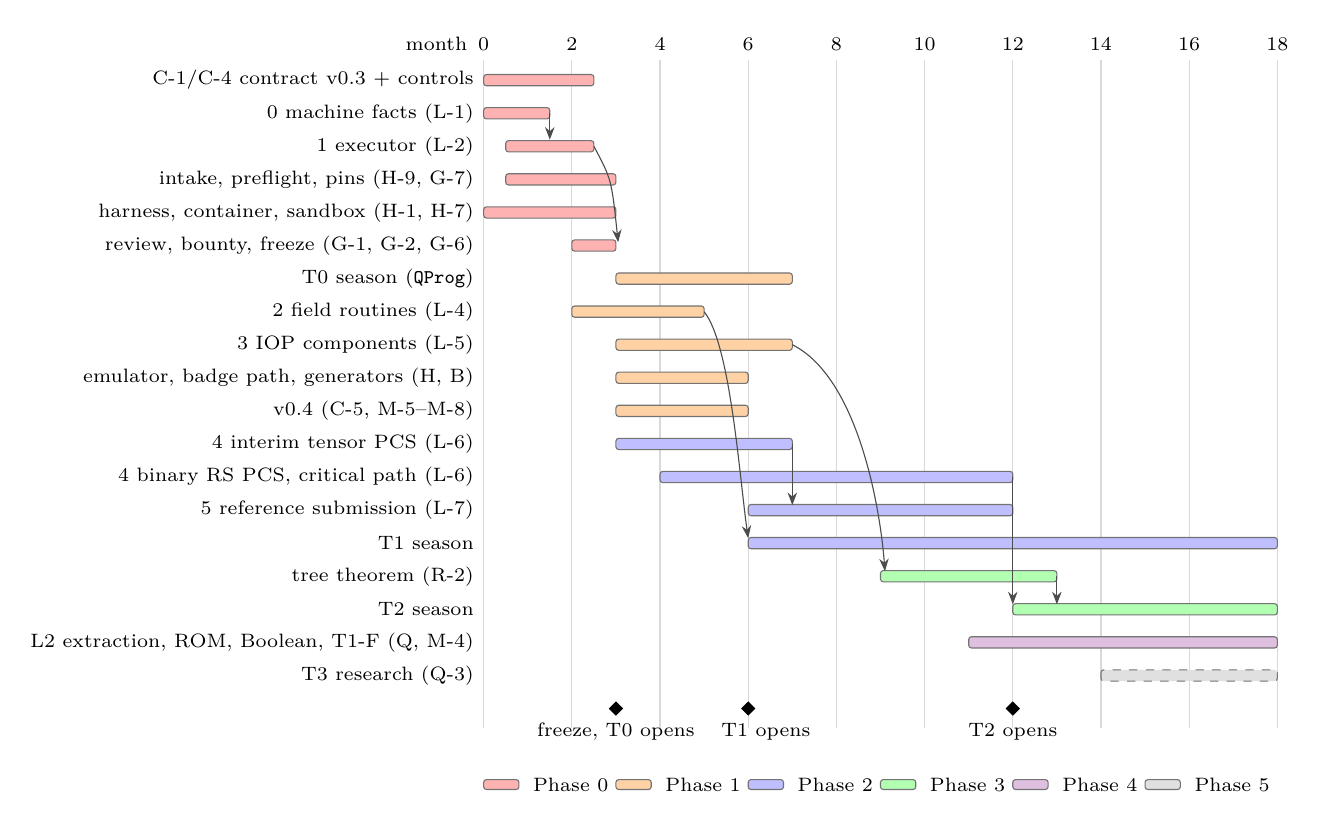
\begin{tikzpicture}[x=0.56cm,y=0.42cm,
  bar/.style={draw=black!55,rounded corners=1pt,minimum height=0.30cm,inner sep=0pt},
  p0/.style={bar,fill=red!30}, p1/.style={bar,fill=orange!35}, p2/.style={bar,fill=blue!25},
  p3/.style={bar,fill=green!30}, p4/.style={bar,fill=violet!25}, p5/.style={bar,fill=black!12},
  lab/.style={anchor=east,font=\scriptsize,inner sep=1pt},
  dep/.style={-{Stealth[length=1.6mm]},draw=black!70,thin},
  ms/.style={draw=black,fill=black,diamond,inner sep=1.2pt}]
% axis
\foreach \m in {0,2,...,18} {
  \draw[black!15] (\m,0.6) -- (\m,-19.6);
  \node[font=\scriptsize,anchor=south] at (\m,0.6) {\m};
}
\node[font=\scriptsize,anchor=south east] at (-0.15,0.6) {month};
% helper: \bar{row}{start}{end}{style}{label}
\newcommand{\gbar}[5]{%
  \draw[#4] (#2,-#1+0.17) rectangle (#3,-#1-0.17);
  \node[lab] at (-0.15,-#1) {#5};}
\gbar{0}{0}{2.5}{p0}{C-1/C-4 contract v0.3 + controls}
\gbar{1}{0}{1.5}{p0}{\libc{0} machine facts (L-1)}
\gbar{2}{0.5}{2.5}{p0}{\libc{1} executor (L-2)}
\gbar{3}{0.5}{3}{p0}{intake, preflight, pins (H-9, G-7)}
\gbar{4}{0}{3}{p0}{harness, container, sandbox (H-1, H-7)}
\gbar{5}{2}{3}{p0}{review, bounty, freeze (G-1, G-2, G-6)}
\gbar{6}{3}{7}{p1}{T0 season (\lean{QProg})}
\gbar{7}{2}{5}{p1}{\libc{2} field routines (L-4)}
\gbar{8}{3}{7}{p1}{\libc{3} IOP components (L-5)}
\gbar{9}{3}{6}{p1}{emulator, badge path, generators (H, B)}
\gbar{10}{3}{6}{p1}{v0.4 (C-5, M-5--M-8)}
\gbar{11}{3}{7}{p2}{\libc{4} interim tensor PCS (L-6)}
\gbar{12}{4}{12}{p2}{\libc{4} binary RS PCS, critical path (L-6)}
\gbar{13}{6}{12}{p2}{\libc{5} reference submission (L-7)}
\gbar{14}{6}{18}{p2}{T1 season}
\gbar{15}{9}{13}{p3}{tree theorem (R-2)}
\gbar{16}{12}{18}{p3}{T2 season}
\gbar{17}{11}{18}{p4}{L2 extraction, ROM, Boolean, T1-F (Q, M-4)}
\draw[p5,dashed] (14,-18+0.17) rectangle (18,-18-0.17);
\node[lab] at (-0.15,-18) {T3 research (Q-3)};
% milestones
\node[ms] (fz) at (3,-19) {}; \node[font=\scriptsize,anchor=north] at (3,-19.15) {freeze, T0 opens};
\node[ms] (t1) at (6,-19) {}; \node[font=\scriptsize,anchor=north] at (6.4,-19.15) {T1 opens};
\node[ms] (t2) at (12,-19) {}; \node[font=\scriptsize,anchor=north] at (12,-19.15) {T2 opens};
% dependencies
\draw[dep] (1.5,-1) -- (1.5,-1.8);
\draw[dep] (2.5,-2) .. controls (2.9,-3) .. (3.05,-4.9);
\draw[dep] (5,-7) .. controls (5.6,-8) and (5.8,-12) .. (6,-13.85);
\draw[dep] (7,-11) -- (7,-12.85);
\draw[dep] (12,-12) -- (12,-15.85);
\draw[dep] (13,-15) -- (13,-15.85);
\draw[dep] (7,-8) .. controls (8.5,-9) and (9,-13) .. (9.1,-14.85);
% phase legend
\begin{scope}[shift={(0,-21.3)}]
\foreach \s/\t/\x in {p0/Phase 0/0, p1/Phase 1/3, p2/Phase 2/6, p3/Phase 3/9, p4/Phase 4/12, p5/Phase 5/15} {
  \draw[\s] (\x,0.15) rectangle (\x+0.8,-0.15);
  \node[font=\scriptsize,anchor=west] at (\x+0.9,0) {\t};
}
\end{scope}
\end{tikzpicture}
\caption{Indicative schedule with the main dependencies (arrows): \libc{0}$\to$\libc{1}$\to$freeze; \libc{2}$\to$T1 opens; interim \libc{4}$\to$\libc{5}; full \libc{4}$\to$T2;
\libc{3}$\to$tree theorem$\to$T2. Months count from the start of Phase~0.}
\label{fig:iss-gantt}
\end{figure}

\paragraph{Reading the plan.} Phase~0 is the only phase whose output is trusted; after the freeze
only security fixes change the contract id (G-2). Its exit criteria include the harness order and the
manifest (vii), because round~3 showed that a correct contract can still certify a false statement
under a wrong build order. The v0.4 items (\cref{tab:iss-v04}) land before T1 with a new
contract id. Phase~1 overlaps the T0 season with the library work T1 needs (A3-S6). Until \libc{4} and
\libc{5} exist, T1 is expected to show only trivial and hybrid entries, so \libc{4}, the critical path,
starts in Phase~1 with the interim tensor-code PCS as a hedge. Phases 4 and 5 enter as versioned
contract extensions with their own controls and baselines.

\FloatBarrier
\begin{takeaway}[Launch-blocking work in one paragraph]
The 15 P0 issues are C-1, C-3, C-4, M-1, M-2, L-1, L-2, H-1, H-7, H-9, G-1, G-2, G-3, G-6 and G-7.
The certified baseline already shows the certificate inhabited and checkable in about 6\,min per
harness run. Before anything opens:
\begin{itemize}[nosep]
\item freeze the v0.3 contract with the round-3 fixes and all controls, including the T0
  certificate; publish the compiled-code policy that the gate already enforces;
\item finish the Zbc differential tests, decide the class set and ship \libc{0}--\libc{1};
\item build the intake (preflight, source policy) and run the harness in the order of Decision~A-3
  under the production sandbox, with the \code{.olean} manifest checked before and after every stage
  and the checker binaries pinned; fix the second-kernel policy;
\item have the release candidate, pipeline included, reviewed once more and offer a bounty;
\item freeze it with versioning and revalidation in place.
\end{itemize}
Everything else, including the v0.4 cost and timer fixes and the critical-path PCS, can follow the T0
launch.
\end{takeaway}
\clearpage


\appendix
% Provenance: copied from the design workspace CambridgePQ/recursion.fast, `report/sections/A-lean-contract.tex`, on 2026-10-19. Read-only copy; the source is authoritative.
% A-lean-contract -- written by W7; listings regenerated from contract-v03 by scripts/regen-appendix-a.py (W10b)
% The group below adds a glyph fallback (e.g. U+2113) to the monospace font of the listings only.
\begingroup
\directlua{luaotfload.add_fallback("rfleanmono", {"DejaVu Sans:mode=node;", "STIX Two Math:mode=node;"})}
\setmonofont{DejaVu Sans Mono}[Scale=0.82,RawFeature={fallback=rfleanmono}]
\section{Lean contract listings}\label{sec:appendix-contract}

This appendix reproduces the trusted contract v0.3 (\code{contract-v03/RecursionFast/Contract/}),
which compiles against Lean v4.34.1 and Mathlib v4.34.1 and imports nothing else except the vendored
riscv-zkvm model. The files appear in the import order of the root module, which is the intended
reading order. Each listing is the \emph{complete} compiled source, generated from it by a script
(\path{report/scripts/regen-appendix-a.py}, which also has a \code{--check} mode for CI), with
three mechanical changes: the module header comment, paraphrased in the paragraph before the
listing, is omitted; the lines \lean{namespace RecursionFast} and \lean{end RecursionFast} that
enclose every file are omitted; and lines longer than 112 characters are broken at a space, with
the continuation indented four further spaces. Nothing is elided. The listings in
\cref{sec:protocol,sec:security} are excerpts of these. For each file the paragraph states what it
defines and what an auditor must check. \Cref{tab:app-loc} gives the line counts, and
\cref{subsec:app-checklist} the auditor's checklist.

\begin{table}[h]
\centering\small
\begin{tabular}{@{}lrrrrl@{}}
\toprule
File & Code & Comment & Blank & Total & v0.2 code \\
\midrule
\code{Field.lean} & 36 & 27 & 20 & 83 & 36 \\
\code{R1CS.lean} & 36 & 31 & 18 & 85 & 41 \\
\code{Shapes.lean} & 50 & 37 & 25 & 112 & 50 \\
\code{Security.lean} & 55 & 38 & 20 & 113 & 55 \\
\code{Protocol.lean} & 27 & 23 & 10 & 60 & 27 \\
\code{Timer.lean} (new) & 22 & 23 & 14 & 59 & -- \\
\code{Machine.lean} & 297 & 117 & 59 & 473 & 165 \\
\code{Agrees.lean} & 18 & 17 & 11 & 46 & 18 \\
\code{Cost.lean} & 73 & 61 & 35 & 169 & 38 \\
\code{QProg.lean} & 21 & 13 & 8 & 42 & 21 \\
\code{Accumulation.lean} & 77 & 48 & 29 & 154 & 72 \\
\code{Certificate.lean} & 72 & 35 & 19 & 126 & 48 \\
\code{Contract.lean} (root) & 12 & 1 & 1 & 14 & 11 \\
\midrule
\textbf{Total} & \textbf{796} & \textbf{471} & \textbf{269} & \textbf{1{,}536} & \textbf{582} \\
\bottomrule
\end{tabular}
\caption{Line counts of the trusted contract after the round-3 fixes (\code{contract-v03/scripts/loc.py},
re-run for this appendix; a line with code and a comment counts as code; doc comments count as comments). Not counted: the vendored riscv-zkvm model, of
which the contract reaches 474 declarations in 930 source lines (205 of them theorems pulled in by
\lean{deriving DecidableEq} on \lean{Instruction}).}
\label{tab:app-loc}
\end{table}

\subsection{Root module}\label{subsec:app-root}

The root module only imports the twelve files. An auditor checks that its import list is the
reading order below and that no file imports anything outside Lean core, Mathlib and
\code{RiscvZkvm} (the closure of \lean{import RecursionFast.Contract} has 2,635 modules and no
ArkLib, CompPoly or VCVio module).

\begin{leancode}[fontsize=\scriptsize,label={\footnotesize RecursionFast/Contract.lean}]
import RecursionFast.Contract.Field
import RecursionFast.Contract.R1CS
import RecursionFast.Contract.Shapes
import RecursionFast.Contract.Security
import RecursionFast.Contract.Protocol
import RecursionFast.Contract.Timer
import RecursionFast.Contract.Machine
import RecursionFast.Contract.Agrees
import RecursionFast.Contract.Cost
import RecursionFast.Contract.QProg
import RecursionFast.Contract.Accumulation
import RecursionFast.Contract.Certificate

/-! # recursion.fast trusted contract v0.3 (root). The imports above are the reading order. -/
\end{leancode}

\subsection{\texttt{Field.lean}: the fields \texorpdfstring{$K$}{K} and \texorpdfstring{$E$}{E}}

$K=\mathbb{F}_2[x]/(x^{64}+x^4+x^3+x+1)$ in the polynomial basis (bit $i$ of a word is the
coefficient of $x^i$), so every 64-bit word is an element and every 8-byte string a canonical
encoding; $E=K[y]/(y^3+y+1)$ as three limbs. Lean core only. The field axioms, $|K|=2^{64}$,
$|E|=2^{192}$, irreducibility of both moduli and the definitional identification with CompPoly's
\lean{BF64} and \lean{BF64.Ext3} are theorems of the untrusted library. \emph{Check}: the reduction
constant \lean{0x1B} is $x^4+x^3+x+1$; two folds suffice (after one fold the degree is below 67);
the $E$ product folds $y^3=y+1$ and $y^4=y^2+y$; the encodings are little-endian, limbs in the order
$c_0,c_1,c_2$; \lean{K.clmul} is also the semantics of Zbc.

\begin{leancode}[fontsize=\scriptsize,label={\footnotesize Contract/Field.lean}]
/-- A 64-bit machine word (also the unit of the tape and of oracle leaves). -/
abbrev Word := BitVec 64

/-- An element of `K = GF(2^64)`: bit `i` of `bits` is the coefficient of `x^i`. -/
structure K where
  bits : Word
  deriving DecidableEq

namespace K

/-- Carry-less product of two polynomials of degree `< 64` over GF(2), as a 128-bit word
(schoolbook shift-and-xor). Also the semantics of the Zbc instructions (`Machine.lean`). -/
def clmul (a b : Word) : BitVec 128 :=
  Fin.foldl 64 (fun acc i => if a.getLsbD i then acc ^^^ (b.zeroExtend 128 <<< (i : Nat)) else acc) 0

/-- One reduction fold `hi·x^64 + lo ↦ hi·(x^4 + x^3 + x + 1) + lo` (`x^64 ≡ 0x1B`). -/
def fold (t : BitVec 128) : BitVec 128 :=
  clmul ((t >>> 64).setWidth 64) 0x1B ^^^ (t.setWidth 64).zeroExtend 128

/-- Reduction modulo `x^64 + x^4 + x^3 + x + 1`: two folds bring the degree below 64. -/
def reduce (t : BitVec 128) : Word := (fold (fold t)).setWidth 64

instance : Zero K := ⟨⟨0⟩⟩
instance : One K := ⟨⟨1⟩⟩
/-- Addition = subtraction = xor (characteristic 2); negation is the identity. -/
instance : Add K := ⟨fun a b => ⟨a.bits ^^^ b.bits⟩⟩
instance : Sub K := ⟨fun a b => ⟨a.bits ^^^ b.bits⟩⟩
instance : Neg K := ⟨fun a => a⟩
/-- Multiplication: carry-less product, then reduction. -/
instance : Mul K := ⟨fun a b => ⟨reduce (clmul a.bits b.bits)⟩⟩

/-- Canonical encoding: the 8 little-endian bytes of `bits` (Rust `u64::to_le_bytes`). On the
machine an element is one doubleword, which memory stores little-endian, i.e. these bytes. -/
def toBytes (a : K) : List (BitVec 8) := List.ofFn fun i : Fin 8 => (a.bits >>> (8 * i.val)).setWidth 8

end K

/-- An element `c0 + c1·y + c2·y²` of `E = K[y]/(y^3 + y + 1) = GF(2^192)`. -/
structure E where
  c0 : K
  c1 : K
  c2 : K
  deriving DecidableEq

namespace E

instance : Zero E := ⟨⟨0, 0, 0⟩⟩
instance : One E := ⟨⟨1, 0, 0⟩⟩
instance : Add E := ⟨fun a b => ⟨a.c0 + b.c0, a.c1 + b.c1, a.c2 + b.c2⟩⟩
/-- Schoolbook product folded by `y^3 = y + 1`, `y^4 = y^2 + y` (9 products in K). -/
instance : Mul E := ⟨fun a b =>
  let p3 := a.c1 * b.c2 + a.c2 * b.c1
  let p4 := a.c2 * b.c2
  ⟨a.c0 * b.c0 + p3, a.c0 * b.c1 + a.c1 * b.c0 + p3 + p4, a.c0 * b.c2 + a.c1 * b.c1 + a.c2 * b.c0 + p4⟩⟩

/-- Canonical encoding as words: limbs `c0, c1, c2` in this order (24 bytes, each limb LE). -/
def toWords (a : E) : List Word := [a.c0.bits, a.c1.bits, a.c2.bits]

/-- Canonical 24-byte encoding: limbs `c0, c1, c2`, each 8 bytes little-endian. -/
def toBytes (a : E) : List (BitVec 8) := a.c0.toBytes ++ a.c1.toBytes ++ a.c2.toBytes

end E
\end{leancode}

\subsection{\texttt{R1CS.lean}: the relation and the size classes}

\lean{Sizes} with $\mathit{cols}=1+n_x+n_w$; the class shape \lean{classSizes k}
($m=\mathit{cols}=2^k$, $n_x=2^{10}$, $\mathit{nnz}\le2^{k+4}$) at \lean{classExp c}${}\in\{16,20,24\}$;
sparse matrices as entry lists (duplicates summed); the index with \lean{nnz\_le} on the list
lengths; $z=(1,x,w)$; \lean{R1CS} and \lean{rel}; and the harness padding maps, whose
satisfiability preservation in both directions is \lean{pad\_sat\_iff} in the library.
\emph{Check}: the constant wire is column 0 (\lean{Fin.cons 1}); \lean{SpMat.mulVec} sums all entries
of row $r$; \lean{R1CS} quantifies over every row; padding keeps public inputs at their columns,
moves witness columns past the larger $n_x$, and pads $x$ with zeros. A statement is a
representation: equal matrices given by different lists are different statements, so the harness
fixes a canonical form for benchmark indices.

\begin{leancode}[fontsize=\scriptsize,label={\footnotesize Contract/R1CS.lean}]
import RecursionFast.Contract.Field
import Mathlib.Data.Fin.Tuple.Basic

/-- Sizes of an R1CS instance: `m` rows, `nx` public inputs, `nw` witness entries, at most
`nnz` nonzero matrix entries in total. Columns: `cols = 1 + nx + nw` (the constant wire first). -/
structure Sizes where
  m : ℕ
  nx : ℕ
  nw : ℕ
  nnz : ℕ
  deriving DecidableEq

/-- Number of columns, `1 + nx + nw`. -/
abbrev Sizes.cols (sz : Sizes) : ℕ := sz.nx + sz.nw + 1

/-- The fixed class shape for exponent `k` (meaningful for `k ≥ 10`): `m = cols = 2^k`. -/
def classSizes (k : ℕ) : Sizes := ⟨2 ^ k, 2 ^ 10, 2 ^ k - 1 - 2 ^ 10, 2 ^ (k + 4)⟩

/-- The three scored classes, by exponent: `classExp 0 = 16`, `classExp 1 = 20`, `classExp 2 = 24`. -/
def classExp (c : Fin 3) : ℕ := 16 + 4 * c.val

/-- A **sparse** matrix: a list of entries `(row, column, value)`, indices in range by typing.
Entries at a repeated position are **summed**: the matrix denoted is the sum of its entries
(`Library/R1CS.lean`: `SpMat.toMat`, and `mulVec` equals Mathlib's dense `Matrix.mulVec`). -/
abbrev SpMat (sz : Sizes) := List (Fin sz.m × Fin sz.cols × K)

/-- Row `r` of the matrix-vector product, `Σ_{(r, c, v) ∈ M} v · z[c]` in K (left to right; the
order is irrelevant since `+` is xor). -/
def SpMat.mulVec {sz : Sizes} (M : SpMat sz) (z : Fin sz.cols → K) (r : Fin sz.m) : K :=
  M.foldl (fun acc e => if e.1 = r then acc + e.2.2 * z e.2.1 else acc) 0

/-- An R1CS index (the circuit): three sparse matrices with at most `nnz` entries in total (so an
indexer runs in time linear in `nnz`, not in `m · cols`). -/
structure Index (sz : Sizes) where
  A : SpMat sz
  B : SpMat sz
  C : SpMat sz
  nnz_le : A.length + B.length + C.length ≤ sz.nnz

/-- Public input `x ∈ K^nx`. -/
abbrev PubInput (sz : Sizes) := Fin sz.nx → K
/-- Witness `w ∈ K^nw`. -/
abbrev Wit (sz : Sizes) := Fin sz.nw → K

/-- The full assignment `z = (1, x, w)`. -/
def zVec {sz : Sizes} (x : PubInput sz) (w : Wit sz) : Fin sz.cols → K := Fin.cons 1 (Fin.append x w)

/-- **The relation**: every row satisfies `(A z)_r · (B z)_r = (C z)_r`. -/
def R1CS {sz : Sizes} (i : Index sz) (x : PubInput sz) (w : Wit sz) : Prop :=
  ∀ r, i.A.mulVec (zVec x w) r * i.B.mulVec (zVec x w) r = i.C.mulVec (zVec x w) r

instance {sz : Sizes} (i : Index sz) (x : PubInput sz) (w : Wit sz) : Decidable (R1CS i x w) :=
  inferInstanceAs (Decidable (∀ _, _))

/-- The relation as a set: statement `(index, public input)`, witness `w`. -/
def rel (sz : Sizes) : Set ((Index sz × PubInput sz) × Wit sz) := {p | R1CS p.1.1 p.1.2 p.2}

/-- Harness padding of an instance of size `sz` into a larger size `sz'` (column map): the
constant column stays at 0, public input `j < nx` stays at column `1 + j`, witness `j < nw` moves
to column `1 + nx' + j`; `none` if it does not fit. Rows keep their number. The padded public
input is `x` followed by zeros. (Satisfiability preservation and reflection: `Library/Pad.lean`.) -/
def padCol (sz sz' : Sizes) (c : Fin sz.cols) : Option (Fin sz'.cols) :=
  let t := if c.val ≤ sz.nx then c.val else c.val - sz.nx + sz'.nx
  if h : t < sz'.cols then some ⟨t, h⟩ else none

/-- The padded matrix: every entry moved by `padCol` (entries that do not fit are dropped). -/
def SpMat.pad {sz : Sizes} (sz' : Sizes) (M : SpMat sz) : SpMat sz' :=
  M.filterMap fun e => if h : e.1.val < sz'.m then (padCol sz sz' e.2.1).map (⟨e.1.val, h⟩, ·, e.2.2) else none

/-- The padded public input: `x` followed by zeros. -/
def PubInput.pad {sz : Sizes} (sz' : Sizes) (x : PubInput sz) : PubInput sz' :=
  fun j => if h : j.val < sz.nx then x ⟨j.val, h⟩ else 0
\end{leancode}

\subsection{\texttt{Shapes.lean}: round shapes, transcripts and oracles}

The fixed round menu (\cref{subsec:proto-rounds}): a prover round sends a raw vector of
$2^{\mathit{logLen}}$ elements of $K$, read in leaves of $2^{\mathit{logLeaf}}$; a verifier round
sends $n_E$ elements of $E$ and one $b$-bit index per $b$ in \lean{idx}. Transcript prefixes are
dependent functions on \lean{Fin m}, as in ArkLib. \emph{Check}: message types are exactly
\lean{OVal o} (no submitter type, so \enquote{for all transcripts} is \enquote{for all oracle
contents}); there are no $K$-valued challenges; \lean{Round.tapeWords} writes an $E$ element as its
three limbs and an index zero-extended to one word, in round order; prover messages become QUERY
oracles $1,2,\dots$ in round order; \lean{Oracle.get} returns $0$ beyond the length, which
\code{QUERY} never reads.

\begin{leancode}[fontsize=\scriptsize,label={\footnotesize Contract/Shapes.lean}]
import RecursionFast.Contract.Field
import Mathlib.Data.Fin.Tuple.Basic

/-- Contract round cap (DESIGN §3/§5): every protocol and reduction has at most `2^14` rounds. -/
def roundCap : ℕ := 2 ^ 14

/-- Shape of an oracle: `2^logLen` elements of K, read in leaves of `2^logLeaf` elements, so a
QUERY opens one of `2^(logLen - logLeaf)` leaves (Merkle depth `logLen - logLeaf`). -/
structure OShape where
  logLen : ℕ
  logLeaf : ℕ
  deriving DecidableEq

/-- Contents of an oracle of shape `o`. -/
abbrev OVal (o : OShape) := Fin (2 ^ o.logLen) → K

/-- A round of the contract's fixed menu. -/
inductive Round where
  /-- The prover sends an oracle of shape `o`. -/
  | msg (o : OShape)
  /-- The verifier sends `nE` elements of E and one `b`-bit index for each `b ∈ idx`. -/
  | chal (nE : ℕ) (idx : List ℕ)
  deriving DecidableEq

/-- What is sent in a round: a raw K-vector, or (E-vector, indices). -/
def Round.Ty : Round → Type
  | .msg o => OVal o
  | .chal nE idx => (Fin nE → E) × ((j : Fin idx.length) → BitVec (idx.get j))

/-- Whether the prover speaks in this round. -/
def Round.isMsg : Round → Bool
  | .msg _ => true
  | .chal _ _ => false

variable {n : ℕ} (sh : Fin n → Round)

/-- Transcript prefix of length `m`: the values of rounds `0, …, m-1`. -/
abbrev Transcript (m : Fin (n + 1)) := (i : Fin m) → (sh (Fin.castLE (Nat.le_of_lt_succ m.isLt) i)).Ty

/-- A full transcript: a value for every round. -/
abbrev FullTranscript := (i : Fin n) → (sh i).Ty

/-- The empty transcript. -/
def Transcript.empty : Transcript sh 0 := fun i => Fin.elim0 i

/-- Append the value of round `m` to a prefix of length `m`. -/
def Transcript.concat {sh : Fin n → Round} {m : Fin n} (tr : Transcript sh m.castSucc) (a : (sh m).Ty) :
    Transcript sh m.succ :=
  Fin.snoc (α := fun i : Fin (m.val + 1) => (sh (Fin.castLE m.isLt i)).Ty) tr a

/-- Indices of prover rounds. -/
abbrev MessageIdx := {m : Fin n // (sh m).isMsg = true}
/-- Indices of verifier (challenge) rounds. -/
abbrev ChallengeIdx := {m : Fin n // (sh m).isMsg = false}
/-- A choice of all challenges. -/
abbrev Challenges := (c : ChallengeIdx sh) → (sh c.1).Ty

/-- An oracle as the machine sees it: a shape and contents. -/
structure Oracle where
  shape : OShape
  data : OVal shape

instance : Inhabited Oracle := ⟨⟨⟨0, 0⟩, fun _ => 0⟩⟩

/-- Element `p` of an oracle (`0` beyond its length; QUERY never reads there). -/
def Oracle.get (o : Oracle) (p : ℕ) : K := if h : p < 2 ^ o.shape.logLen then o.data ⟨p, h⟩ else 0

/-- Number of leaves, `2^(logLen - logLeaf)`. -/
def OShape.leaves (o : OShape) : ℕ := 2 ^ (o.logLen - o.logLeaf)

/-- Leaf `l`: elements `l·2^logLeaf, …, (l+1)·2^logLeaf - 1`. -/
def Oracle.leaf (o : Oracle) (l : ℕ) : List K :=
  List.ofFn fun t : Fin (2 ^ o.shape.logLeaf) => o.get (l * 2 ^ o.shape.logLeaf + t.val)

/-- The oracles a round contributes (one for a `msg` round). -/
def Round.oracles : (r : Round) → r.Ty → List Oracle
  | .msg o, v => [⟨o, v⟩]
  | .chal _ _, _ => []

/-- The tape words a round contributes: E elements as 3 limbs each, then each index
zero-extended to one word (`b ≤ 64` is an admission rule). Prover rounds contribute none. -/
def Round.tapeWords : (r : Round) → r.Ty → List Word
  | .msg _, _ => []
  | .chal nE idx, (es, is) =>
      (List.ofFn fun j : Fin nE => (es j).toWords).flatten ++
        List.ofFn fun j : Fin idx.length => (is j).setWidth 64

/-- The prover messages of a transcript, as oracles `1, 2, …` in round order. -/
def FullTranscript.oracles {sh : Fin n → Round} (tr : FullTranscript sh) : List Oracle :=
  (List.ofFn fun i => (sh i).oracles (tr i)).flatten

/-- The challenges of a transcript, as tape words in round order. -/
def FullTranscript.tapeWords {sh : Fin n → Round} (tr : FullTranscript sh) : List Word :=
  (List.ofFn fun i => (sh i).tapeWords (tr i)).flatten
\end{leancode}

\subsection{\texttt{Security.lean}: completeness and round-by-round knowledge soundness}

The definitions of \cref{sec:security}, over the contract's round shapes and Mathlib only: a
deterministic \lean{Strategy}, a pure verifier, the honest transcript built by
\lean{Fin.induction}, \lean{PerfectComplete} for every challenge vector, the backward
\lean{Extractor}, the knowledge state function with its three laws, \lean{KSF.Bad}, \lean{RbrKS} in
counting form and \lean{SecureWith} with the error cap. \emph{Check}: \lean{Transcript sh m} is the
prefix of length $m$, so \lean{m.castSucc} and \lean{m.succ} are before and after round $m$;
\lean{cast E.eqIn} is an identity coercion; the $\exists w$ in \lean{Bad} ranges over next-stage
witnesses; the worst case is over every statement, challenge round and prefix; \lean{Nat.card} is
the size of a finite, non-empty challenge type; \lean{errorCap} is $2^{-128}$ (control
\lean{errorCap\_lt\_one}). At L1 \lean{RbrKS} is equivalent to RBR soundness
(\cref{thm:sec-collapse}).

\begin{leancode}[fontsize=\scriptsize,label={\footnotesize Contract/Security.lean}]
import RecursionFast.Contract.Shapes
import Mathlib.Basic.NNReal.Defs
import Mathlib.SetTheory.Cardinal.Finite

open scoped NNReal

/-- Contract error cap (DESIGN §5): every round's error is at most `2^-128`. -/
noncomputable def errorCap : ℝ≥0 := (2 : ℝ≥0)⁻¹ ^ 128

variable {n : ℕ} (sh : Fin n → Round) (Stmt Wit StmtOut WitOut : Type)

/-- A deterministic prover: each message is a function of the input and the transcript so far;
the output (statement, witness) is a function of the full transcript. -/
structure Strategy where
  next : Stmt → Wit → (m : MessageIdx sh) → Transcript sh m.1.castSucc → (sh m.1).Ty
  output : Stmt → Wit → FullTranscript sh → StmtOut × WitOut

/-- A pure verifier: a total function of the statement and the full transcript; `none` = reject. -/
abbrev PureVerifier := Stmt → FullTranscript sh → Option StmtOut

variable {sh Stmt Wit StmtOut WitOut}

/-- The honest transcript prefixes on challenge vector `ρ`: round `j` is the prover's message if
`j` is a prover round, and `ρ`'s entry otherwise. -/
def Strategy.prefixes (P : Strategy sh Stmt Wit StmtOut WitOut) (s : Stmt) (w : Wit)
    (ρ : Challenges sh) : (m : Fin (n + 1)) → Transcript sh m :=
  Fin.induction (Transcript.empty sh) fun j tr =>
    tr.concat (if h : (sh j).isMsg then P.next s w ⟨j, h⟩ tr else ρ ⟨j, by simpa using h⟩)

/-- The full honest transcript on challenge vector `ρ`. -/
def Strategy.transcript (P : Strategy sh Stmt Wit StmtOut WitOut) (s : Stmt) (w : Wit)
    (ρ : Challenges sh) : FullTranscript sh :=
  P.prefixes s w ρ (Fin.last n)

/-- **Perfect completeness**: for every `(s, w) ∈ relIn` and every challenge vector, the verifier
accepts the honest transcript with the prover's output statement, and the output pair is in
`relOut`. -/
def PerfectComplete (relIn : Set (Stmt × Wit)) (relOut : Set (StmtOut × WitOut))
    (P : Strategy sh Stmt Wit StmtOut WitOut) (V : PureVerifier sh Stmt StmtOut) : Prop :=
  ∀ s w, (s, w) ∈ relIn → ∀ ρ : Challenges sh,
    V s (P.transcript s w ρ) = some (P.output s w (P.transcript s w ρ)).1 ∧
      P.output s w (P.transcript s w ρ) ∈ relOut

variable (sh Stmt Wit WitOut) in
/-- A round-by-round extractor with intermediate witness types `WitMid` (ArkLib's
`Extractor.RoundByRound`): `extractMid m` maps a witness after round `m` to one before it. -/
structure Extractor (WitMid : Fin (n + 1) → Type) where
  eqIn : WitMid 0 = Wit
  extractMid : (m : Fin n) → Stmt → Transcript sh m.succ → WitMid m.succ → WitMid m.castSucc
  extractOut : Stmt → FullTranscript sh → WitOut → WitMid (Fin.last n)

/-- A **knowledge state function** for `V` and the named extractor `E`. Laws: `empty` (before
round 0 the state is the input relation), `next` (a prover message cannot make the state true
unless it was true before, with the extracted witness), `full` (an accepted full transcript with
an output pair in `relOut` makes the state true with the extracted final witness). -/
structure KSF (relIn : Set (Stmt × Wit)) (relOut : Set (StmtOut × WitOut))
    (V : PureVerifier sh Stmt StmtOut) {WitMid : Fin (n + 1) → Type}
    (E : Extractor sh Stmt Wit WitOut WitMid) where
  toFun : (m : Fin (n + 1)) → Stmt → Transcript sh m → WitMid m → Prop
  empty : ∀ s w, (s, cast E.eqIn w) ∈ relIn ↔ toFun 0 s (Transcript.empty sh) w
  next : ∀ (m : MessageIdx sh) s (tr : Transcript sh m.1.castSucc) (msg : (sh m.1).Ty) w,
    toFun m.1.succ s (tr.concat msg) w → toFun m.1.castSucc s tr (E.extractMid m.1 s (tr.concat msg) w)
  full : ∀ s tr sOut wOut, V s tr = some sOut → (sOut, wOut) ∈ relOut →
    toFun (Fin.last n) s tr (E.extractOut s tr wOut)

variable {relIn : Set (Stmt × Wit)} {relOut : Set (StmtOut × WitOut)}
  {V : PureVerifier sh Stmt StmtOut} {WitMid : Fin (n + 1) → Type}
  {E : Extractor sh Stmt Wit WitOut WitMid}

/-- A fresh challenge `ch` in round `c` is **bad** for prefix `tr` if some witness makes the state
true after `ch` while the extracted witness does not make it true before `ch`. -/
def KSF.Bad (kSF : KSF relIn relOut V E) (c : ChallengeIdx sh) (s : Stmt)
    (tr : Transcript sh c.1.castSucc) (ch : (sh c.1).Ty) : Prop :=
  ∃ w, ¬ kSF.toFun c.1.castSucc s tr (E.extractMid c.1 s (tr.concat ch) w) ∧
    kSF.toFun c.1.succ s (tr.concat ch) w

/-- **Worst-case RBR knowledge soundness with errors `ε`**, counting form: for every statement,
challenge round and prefix, at most an `ε c`-fraction of the round's challenges is bad. (All
challenge types are finite and nonempty, `Library/Field.lean`, so `Nat.card` is the size.) -/
def RbrKS (kSF : KSF relIn relOut V E) (ε : ChallengeIdx sh → ℝ≥0) : Prop :=
  ∀ s (c : ChallengeIdx sh) (tr : Transcript sh c.1.castSucc),
    (Nat.card {ch // kSF.Bad c s tr ch} : ℝ≥0) ≤ ε c * Nat.card (sh c.1).Ty

/-- The security clause shared by protocols and reductions: perfect completeness, an RBR-KS
state function for the named extractor at errors `ε`, and the error cap `ε c ≤ 2^-128`. -/
structure SecureWith (relIn : Set (Stmt × Wit)) (relOut : Set (StmtOut × WitOut))
    (P : Strategy sh Stmt Wit StmtOut WitOut) (V : PureVerifier sh Stmt StmtOut)
    (E : Extractor sh Stmt Wit WitOut WitMid) (ε : ChallengeIdx sh → ℝ≥0) : Prop where
  complete : PerfectComplete relIn relOut P V
  sound : ∃ kSF : KSF relIn relOut V E, RbrKS kSF ε
  cap : ∀ c, ε c ≤ errorCap
\end{leancode}

\subsection{\texttt{Protocol.lean}: holographic protocols}

A base-track protocol for one size: at most \lean{roundCap} rounds of the menu, a key of at most
\lean{vkCap}${}=2^{10}$ elements, an index oracle of a declared shape, an honest prover, the spec
verifier's decision from $(\mathsf{VK}\,i,x,\mathsf{IDX}\,i,\mathrm{tr})$, a named extractor and
declared errors. \emph{Check}: \lean{verify} never receives the index $i$; \lean{Secure} uses the
contract relation \lean{rel sz}, output relation \lean{Set.univ} and the declared errors.
Computability of the badge-path fields \lean{VK}, \lean{IDX}, \lean{prover} and \lean{extractor}
is a gate check (rule~4), not a Lean property; since round~4 the other fields, \lean{ε} included, may
be \lean{noncomputable} (A7-M2, \code{NOTICE-P2e.md}). The check only guarantees that compiled code
exists: a brute-force indexer is computable, and feasibility is the badge path's job (A7-M1). The
index-oracle cap $2^{k+8}$ is an admission clause in \code{Cost.lean}.

\begin{leancode}[fontsize=\scriptsize,label={\footnotesize Contract/Protocol.lean}]
import RecursionFast.Contract.Security
import RecursionFast.Contract.R1CS

open scoped NNReal

/-- Contract cap on the verification key: at most `2^10` K-elements. -/
def vkCap : ℕ := 2 ^ 10

/-- A holographic public-coin IOP for `rel sz`. -/
structure Protocol (sz : Sizes) where
  /-- Number of rounds, at most `roundCap = 2^14`. -/
  n : ℕ
  n_le : n ≤ roundCap
  /-- The round shapes (contract menu). -/
  shape : Fin n → Round
  /-- Verification key length and the (honest, computable) key. -/
  vkLen : ℕ
  vkLen_le : vkLen ≤ vkCap
  VK : Index sz → (Fin vkLen → K)
  /-- The index oracle (oracle 0): its shape and the (honest, computable) indexer. -/
  idxShape : OShape
  IDX : Index sz → OVal idxShape
  /-- The honest prover. -/
  prover : Strategy shape (Index sz × PubInput sz) (Wit sz) Unit Unit
  /-- The spec verifier's decision, from `VK i`, `x`, `IDX i` and the full transcript. -/
  verify : (Fin vkLen → K) → PubInput sz → OVal idxShape → FullTranscript shape → Bool
  /-- The named round-by-round extractor. -/
  WitMid : Fin (n + 1) → Type
  extractor : Extractor shape (Index sz × PubInput sz) (Wit sz) Unit WitMid
  /-- Declared per-round errors. -/
  ε : ChallengeIdx shape → ℝ≥0

namespace Protocol
variable {sz : Sizes} (P : Protocol sz)

/-- The verifier as a pure verifier on the statement `(i, x)`; `i` enters only via `VK i`, `IDX i`. -/
def specVerifier : PureVerifier P.shape (Index sz × PubInput sz) Unit :=
  fun s tr => if P.verify (P.VK s.1) s.2 (P.IDX s.1) tr then some () else none

/-- **Security of a protocol**: perfect completeness for `rel sz`, worst-case RBR knowledge
soundness with the named extractor at the declared errors, and `ε ≤ 2^-128` in every round
(the round cap `n ≤ 2^14` is a field of `Protocol`). -/
def Secure : Prop :=
  SecureWith (rel sz) Set.univ P.prover P.specVerifier P.extractor P.ε

end Protocol
\end{leancode}

\subsection{\texttt{Timer.lean}: the latency board's pipeline timer}

New in v0.3 (\cref{subsec:cost-lat}): a deterministic in-order dual-issue scoreboard. An operation
issues in the first free slot at or after the cycle in which its sources are ready, its result is
ready \lean{lat} cycles later, and a bubble \lean{pen} (taken branch or jump: 5; \code{QUERY}: 1,560
cycles per Merkle level plus the leaf length) flushes the rest of the cycle. \emph{Check}: the
timer is pure accounting and is never read by the decision; the constants match
\cref{subsec:cost-lat}. Its composition theorem $\mathit{time}(a\mathbin{+\!\!+}b)\le
\mathit{time}\,a+\mathit{time}\,b+L_{\max}$ is in \code{Library/Timer.lean}.

\begin{leancode}[fontsize=\scriptsize,label={\footnotesize Contract/Timer.lean}]
/-- One scheduled operation: destination register (none for `x0`/no result), source registers,
result latency in cycles, and the issue bubble after it in cycles. -/
structure Op where
  dst : Option Nat
  srcs : List Nat
  lat : Nat
  pen : Nat

/-- Scoreboard: the next free issue slot, and per register the cycle its value is ready. -/
structure SB where
  slot : Nat
  ready : Nat → Nat

/-- A fresh pipeline whose clock starts at cycle `t` (every register ready at `t`). -/
def SB.start (t : Nat) : SB := ⟨2 * t, fun _ => t⟩

/-- Elapsed cycles: the cycle after the last occupied slot. -/
def SB.time (sb : SB) : Nat := (sb.slot + 1) / 2

/-- Issue one operation (in order: never before `slot`; after its sources are ready). -/
def SB.step (sb : SB) (o : Op) : SB :=
  let t := o.srcs.foldl (fun m r => max m (2 * sb.ready r)) sb.slot
  { slot := if o.pen = 0 then t + 1 else 2 * (t / 2 + 1 + o.pen)
    ready := fun r => if o.dst = some r then t / 2 + o.lat else sb.ready r }

/-- Stall until cycle `t` (a `JOIN` waiting for its child). -/
def SB.wait (sb : SB) (t : Nat) : SB := { sb with slot := max sb.slot (2 * t) }

/-- Maximum result latency (the composition slack). -/
def Lmax : Nat := 16

/-- Bubble after a taken branch or a jump (D4 §2b `inord`: mispredict 5, static not-taken). -/
def TAKEN_PENALTY : Nat := 5

/-- Pipeline cycles per Merkle level of a QUERY on the latency board (D4 §1.2: software
BLAKE2s compression on the in-order model, 1,560 cycles). -/
def QUERY_LEVEL_CYCLES : Nat := 1560

/-- Fork-join overheads in cycles (D4 §3.2: a pooled runtime, about 1 µs at 2 GHz). -/
def C_SPAWN : Nat := 2000
def C_JOIN : Nat := 2000
\end{leancode}

\subsection{\texttt{Machine.lean}: the RISC-V oracle machine}

The largest file (297 code lines; v0.2: 165). Base instruction semantics and decoder are vendored;
the file adds the constants and memory map, the image, the 18-counter \lean{CostVec}, the decoder
arms for \code{ECALL}, Zbc and the W-ops, their semantics, the memory checks, \code{QUERY} in
closed form, the cost classes and pipeline operations, the shared accounting with first-touch
sets, fork-join harts, \lean{execute}, the initial state and \lean{run}. The module header
(omitted) is the specification restated in \cref{subsec:proto-machine}: system calls by \code{t0}
(0 \code{HALT}, 1 \code{QUERY}, 2 \code{HASH} reserved and trapping, 3 \code{SPAWN}, 4 \code{JOIN}
only with \lean{img.harts}), the memory map, fuel $2^{36}$ per hart with exhaustion rejecting, and
the separation of decision and accounting. \emph{Check}: \lean{decodeInstruction} accepts
\code{ECALL} only as the exact word and never \code{EBREAK} or CSR instructions; the Zbc
(\code{funct7}${}=5$) and W-op encodings; W-op division by zero and shift masking follow the ISA;
loads and stores are naturally aligned, inside $2^{36}$ bytes, and stores miss the tape window;
\code{QUERY} writes exactly the leaf and checks oracle, leaf and destination; \lean{HALT} accepts
only with $a_0=1$ and no live child; in \lean{execute} no \lean{if} or \lean{match} reads the
accounting \lean{x} or the timer \lean{sb}, except the spawn counter \lean{xc.spawns} (handles and
the $2^{16}$ cap); \lean{Ctx.allows} implements the hart discipline (own region, live children's
regions); a child that fails rejects the run; \lean{Acct.vec} counts a written page twice;
\lean{initState} places data at 0, the tape at \lean{TAPE\_BASE}, $\mathit{sp}=2^{36}$. Fuel is per
hart: a child runs with its parent's remaining fuel and the parent is not charged for the child's
steps, so a run with harts may execute up to $(\#\mathrm{spawns}+1)\cdot2^{36}$ steps (A6-F1,
row H12 of \cref{tab:thr-catalogue}).

\begin{leancode}[fontsize=\scriptsize,label={\footnotesize Contract/Machine.lean}]
import RiscvZkvm.Rv64.Execution
import RiscvZkvm.Interpreter.Decode
import RecursionFast.Contract.Shapes
import RecursionFast.Contract.Timer
import Mathlib.Data.Finset.Card
import Mathlib.Order.Interval.Finset.Nat

open RiscvZkvm.Rv64 (MachineState Instr Reg execInstrBr signExtend12)
open RiscvZkvm.Interpreter (decode regOfBits)

/-! ### Constants, image, counters -/

/-- Data memory size: addresses `[0, 2^36)` (bytes). -/
def MEM_BYTES : ℕ := 2 ^ 36
/-- Address of the first instruction (separate code space: loads and stores never reach it). -/
def CODE_BASE : ℕ := 0x1000
/-- Start of the read-only tape. -/
def TAPE_BASE : ℕ := 2 ^ 32
/-- Size of the read-only window at `TAPE_BASE` (= the tape admission cap, 1 MiB). -/
def TAPE_CAP : ℕ := 2 ^ 20
/-- Where a T2 program leaves its output accumulator's plain part (one word per K-element). -/
def OUT_BASE : ℕ := 2 ^ 33
/-- Step limit per hart; running out rejects. -/
def FUEL : ℕ := 2 ^ 36

/-- A program: raw instruction words, data words loaded at address 0, and whether it uses
fork-join harts (`SPAWN`/`JOIN`; if not, they trap as in v0.2). -/
structure Image where
  code : List (BitVec 32)
  data : List Word
  harts : Bool := false

/-- `k` little-endian `w`-bit words packed into the natural `x` (how the challenge renderer
encodes the submitted image files). -/
def unpack (w : ℕ) : ℕ → ℕ → List ℕ
  | 0, _ => []
  | k + 1, x => x % 2 ^ w :: unpack w k (x / 2 ^ w)

/-- Size in bytes (admission cap `2^20`, `Certificate.lean`). -/
def Image.byteSize (img : Image) : ℕ := 4 * img.code.length + 8 * img.data.length

/-- The 18 counters of a run (DESIGN §15.1, D4 §2a, §4.2): instructions by class (`add`:
add/sub/addi/lui/auipc and W forms; `logic`: and/or/xor/slt*; `shift`; `mul`: MUL/MULH*/MULW;
`div`: DIV*/REM* and W forms; `clmul`: Zbc; `ld`/`st`: doubleword, `ldsub`/`stsub`: narrower;
`br`: conditional branches; `jmp`: JAL/JALR), `sys` (HALT, SPAWN, JOIN), first-touched
doublewords `mWords` and 1 KiB pages `mPages` (code and data; a written page counts twice),
and QUERY count / Merkle levels / leaf bytes. -/
structure CostVec where
  add : ℕ := 0
  logic : ℕ := 0
  shift : ℕ := 0
  mul : ℕ := 0
  div : ℕ := 0
  clmul : ℕ := 0
  ld : ℕ := 0
  ldsub : ℕ := 0
  st : ℕ := 0
  stsub : ℕ := 0
  br : ℕ := 0
  jmp : ℕ := 0
  sys : ℕ := 0
  mWords : ℕ := 0
  mPages : ℕ := 0
  qCount : ℕ := 0
  qLevels : ℕ := 0
  qBytes : ℕ := 0
  deriving DecidableEq, Repr

/-- Instruction cost classes (the first twelve counters). -/
inductive Kind where
  | add | logic | shift | mul | div | clmul | ld | ldsub | st | stsub | br | jmp

/-- Count one instruction of class `k`. -/
def CostVec.tick (c : CostVec) : Kind → CostVec
  | .add => { c with add := c.add + 1 } | .logic => { c with logic := c.logic + 1 }
  | .shift => { c with shift := c.shift + 1 } | .mul => { c with mul := c.mul + 1 }
  | .div => { c with div := c.div + 1 } | .clmul => { c with clmul := c.clmul + 1 }
  | .ld => { c with ld := c.ld + 1 } | .ldsub => { c with ldsub := c.ldsub + 1 }
  | .st => { c with st := c.st + 1 } | .stsub => { c with stsub := c.stsub + 1 }
  | .br => { c with br := c.br + 1 } | .jmp => { c with jmp := c.jmp + 1 }

/-- Count one QUERY to an oracle of shape `o`: one Merkle path of depth `logLen - logLeaf` and
`8·2^logLeaf` leaf bytes. -/
def CostVec.addQuery (c : CostVec) (o : OShape) : CostVec :=
  { c with qCount := c.qCount + 1, qLevels := c.qLevels + (o.logLen - o.logLeaf),
           qBytes := c.qBytes + 8 * 2 ^ o.logLeaf }

/-! ### Decoding -/

/-- W-suffixed operations (upstream decodes only `ADDIW`). -/
inductive WordOp where
  | add | sub | sll | srl | sra | mul | div | divu | rem | remu
  deriving DecidableEq

/-- Zbc carry-less multiplications. -/
inductive ClOp where
  | clmul | clmulh | clmulr
  deriving DecidableEq

/-- A decoded instruction: upstream's, a W-op (register or immediate shift), or Zbc. -/
inductive Instruction where
  | base (i : Instr)
  | word (op : WordOp) (rd rs1 rs2 : Reg)
  | wordShift (op : WordOp) (rd rs1 : Reg) (shamt : BitVec 5)
  | cl (op : ClOp) (rd rs1 rs2 : Reg)
  deriving DecidableEq

/-- Decode a raw word: `ECALL` exactly (no `EBREAK`, no CSR), Zbc (`OP`, `funct7 = 5`,
`funct3 = 1/3/2`), the W-ops (`OP-32`, and `OP-IMM-32` shifts), then upstream `decode`. -/
def decodeInstruction (w : BitVec 32) : Option Instruction :=
  let opcode := (w.extractLsb' 0 7).toNat
  let rd := regOfBits (w.extractLsb' 7 5)
  let rs1 := regOfBits (w.extractLsb' 15 5)
  let rs2 := regOfBits (w.extractLsb' 20 5)
  let f3 := (w.extractLsb' 12 3).toNat
  let f7 := (w.extractLsb' 25 7).toNat
  if opcode = 0x73 then (if w = 0x00000073 then some (.base .ECALL) else none)
  else if opcode = 0x33 ∧ f7 = 5 then
    (match f3 with | 1 => some ClOp.clmul | 3 => some .clmulh | 2 => some .clmulr | _ => none).map
      fun op => .cl op rd rs1 rs2
  else if opcode = 0x3b then
    (match f7, f3 with
      | 0, 0 => some WordOp.add | 0x20, 0 => some .sub | 0, 1 => some .sll | 0, 5 => some .srl
      | 0x20, 5 => some .sra | 1, 0 => some .mul | 1, 4 => some .div | 1, 5 => some .divu
      | 1, 6 => some .rem | 1, 7 => some .remu | _, _ => none).map fun op => .word op rd rs1 rs2
  else if opcode = 0x1b ∧ f3 ≠ 0 then
    (match f7, f3 with
      | 0, 1 => some WordOp.sll | 0, 5 => some .srl | 0x20, 5 => some .sra | _, _ => none).map
      fun op => .wordShift op rd rs1 (w.extractLsb' 20 5)
  else (decode w).map .base

/-- 32-bit result of a W-op (RISC-V: shifts use 5 bits; `x/0 = -1`, `x % 0 = x`). -/
def wordResult (op : WordOp) (a b : BitVec 32) : BitVec 32 :=
  match op with
  | .add => a + b | .sub => a - b
  | .sll => a <<< (b.toNat % 32) | .srl => a >>> (b.toNat % 32) | .sra => a.sshiftRight (b.toNat % 32)
  | .mul => a * b
  | .div => if b = 0 then BitVec.allOnes 32 else a.sdiv b
  | .divu => if b = 0 then BitVec.allOnes 32 else a / b
  | .rem => if b = 0 then a else a.srem b
  | .remu => if b = 0 then a else a % b

/-- Zbc: low, high, and reversed (bits 126..63) halves of the 128-bit carry-less product. -/
def clResult (op : ClOp) (a b : Word) : Word :=
  match op with
  | .clmul => (K.clmul a b).setWidth 64
  | .clmulh => (K.clmul a b >>> 64).setWidth 64
  | .clmulr => (K.clmul a b >>> 63).setWidth 64

/-! ### One step -/

/-- `[a, a + len)` lies in data memory. -/
def inMemory (a len : ℕ) : Bool := a + len ≤ MEM_BYTES

/-- `[a, a + len)` lies in data memory and misses the read-only tape window. -/
def writable (a len : ℕ) : Bool :=
  inMemory a len && (a + len ≤ TAPE_BASE || TAPE_BASE + TAPE_CAP ≤ a)

/-- Address, width and direction (`true` = store) of each load and store. -/
def memAccess (s : MachineState) : Instr → Option (Word × ℕ × Bool)
  | .LD _ r o => some (s.getReg r + signExtend12 o, 8, false)
  | .LW _ r o | .LWU _ r o => some (s.getReg r + signExtend12 o, 4, false)
  | .LH _ r o | .LHU _ r o => some (s.getReg r + signExtend12 o, 2, false)
  | .LB _ r o | .LBU _ r o => some (s.getReg r + signExtend12 o, 1, false)
  | .SD r _ o => some (s.getReg r + signExtend12 o, 8, true)
  | .SW r _ o => some (s.getReg r + signExtend12 o, 4, true)
  | .SH r _ o => some (s.getReg r + signExtend12 o, 2, true)
  | .SB r _ o => some (s.getReg r + signExtend12 o, 1, true)
  | _ => none

/-- One non-`ECALL` instruction; `none` is a fault (misaligned or out-of-range access, store
into the tape, `EBREAK`/CSR/pseudo-instructions, which the decoder never produces anyway). -/
def ordinaryStep (s : MachineState) : Instruction → Option MachineState
  | .base .ECALL | .base .EBREAK | .base (.CSRS _ _) | .base (.LI _ _) | .base (.MV _ _)
  | .base .NOP => none
  | .base i =>
    match memAccess s i with
    | some (a, width, store) =>
      if a.toNat % width = 0 && (if store then writable a.toNat width else inMemory a.toNat width)
      then some (execInstrBr s i) else none
    | none => some (execInstrBr s i)
  | .word op rd rs1 rs2 =>
    let v := wordResult op ((s.getReg rs1).truncate 32) ((s.getReg rs2).truncate 32)
    some ((s.setReg rd (v.signExtend 64)).setPC (s.pc + 4))
  | .wordShift op rd rs1 sh =>
    let v := wordResult op ((s.getReg rs1).truncate 32) (sh.zeroExtend 32)
    some ((s.setReg rd (v.signExtend 64)).setPC (s.pc + 4))
  | .cl op rd rs1 rs2 => some ((s.setReg rd (clResult op (s.getReg rs1) (s.getReg rs2))).setPC (s.pc + 4))

/-- Fetch at `pc` (4-aligned, at or above `CODE_BASE`) and decode. -/
def fetch (img : Image) (s : MachineState) : Option Instruction :=
  if CODE_BASE ≤ s.pc.toNat ∧ s.pc.toNat % 4 = 0 then
    (img.code[(s.pc.toNat - CODE_BASE) / 4]?).bind decodeInstruction
  else none

/-- QUERY (see the header). Memory after the call, in closed form: the destination words hold
the leaf, every other word is unchanged. Returns the new state and the oracle's shape. -/
def query (os : List Oracle) (s : MachineState) : Option (MachineState × OShape) := do
  let o ← os[(s.getReg .x10).toNat]?
  let l := (s.getReg .x11).toNat
  let dst := (s.getReg .x12).toNat
  let bytes := 8 * 2 ^ o.shape.logLeaf
  if l < o.shape.leaves ∧ dst % 8 = 0 ∧ writable dst bytes = true then
    some ({ s with
      mem := fun a => if dst ≤ a.toNat ∧ a.toNat < dst + bytes
        then (o.get (l * 2 ^ o.shape.logLeaf + (a.toNat - dst) / 8)).bits else s.mem a
      pc := s.pc + 4 }, o.shape)
  else none

/-! ### Cost classes and pipeline operations -/

/-- The raw word at `pc` (only consulted after `fetch` succeeded). -/
def rawAt (img : Image) (s : MachineState) : BitVec 32 :=
  (img.code[(s.pc.toNat - CODE_BASE) / 4]?).getD 0

/-- Cost class of an instruction (`ECALL` is counted as `sys`; `FENCE` as `add`). -/
def kind : Instruction → Kind
  | .base i =>
    match i with
    | .ADD .. | .SUB .. | .ADDI .. | .LUI .. | .AUIPC .. | .ADDIW .. => .add
    | .AND .. | .OR .. | .XOR .. | .SLT .. | .SLTU .. | .ANDI .. | .ORI .. | .XORI .. | .SLTI .. | .SLTIU .. =>
        .logic
    | .SLL .. | .SRL .. | .SRA .. | .SLLI .. | .SRLI .. | .SRAI .. => .shift
    | .MUL .. | .MULH .. | .MULHSU .. | .MULHU .. => .mul
    | .DIV .. | .DIVU .. | .REM .. | .REMU .. => .div
    | .LD .. => .ld
    | .LW .. | .LWU .. | .LH .. | .LHU .. | .LB .. | .LBU .. => .ldsub
    | .SD .. => .st
    | .SW .. | .SH .. | .SB .. => .stsub
    | .BEQ .. | .BNE .. | .BLT .. | .BGE .. | .BLTU .. | .BGEU .. => .br
    | .JAL .. | .JALR .. => .jmp
    | _ => .add
  | .word op .. => match op with | .add | .sub => .add | .sll | .srl | .sra => .shift | .mul => .mul | _ => .div
  | .wordShift .. => .shift
  | .cl .. => .clmul

/-- Result latency per class in cycles (D4 §2b `inord`, SiFive-7-like: loads, `mul`, `clmul` 3,
`div` 16, everything else 1). -/
def latency : Kind → ℕ
  | .mul | .clmul | .ld | .ldsub => 3
  | .div => 16
  | _ => 1

/-- The pipeline operation of a raw word: destination and sources from its format (`x0` is never
a destination), result latency `lat`, bubble `pen`. -/
def opOf (w : BitVec 32) (lat pen : ℕ) : Op :=
  let f (lo : ℕ) := (w.extractLsb' lo 5).toNat
  let d := if f 7 = 0 then none else some (f 7)
  let (dst, srcs) : Option ℕ × List ℕ := match (w.extractLsb' 0 7).toNat with
    | 0x33 | 0x3b => (d, [f 15, f 20])
    | 0x13 | 0x1b | 0x03 | 0x67 => (d, [f 15])
    | 0x23 | 0x63 => (none, [f 15, f 20])
    | 0x37 | 0x17 | 0x6f => (d, [])
    | _ => (none, [5, 10, 11, 12, 13, 14, 15, 16])
  ⟨dst, srcs, lat, pen⟩

/-- A system call reads `t0, a0, …, a6`; `SPAWN` writes `a0`. -/
def ecallOp (dst : Option ℕ) (pen : ℕ) : Op := ⟨dst, [5, 10, 11, 12, 13, 14, 15, 16], 1, pen⟩

/-! ### Accounting (shared by all harts of a run; never consulted by the decision) -/

/-- Key of a doubleword or page number `n`: data `2n`, code `2n+1` (Harvard: separate spaces). -/
def key (code : Bool) (n : ℕ) : ℕ := 2 * n + if code then 1 else 0

/-- Counters, first-touch sets (doublewords, pages, written pages), pipeline work `W`, spawns. -/
structure Acct where
  cost : CostVec := {}
  words : Finset ℕ := ∅
  pages : Finset ℕ := ∅
  dirty : Finset ℕ := ∅
  work : ℕ := 0
  spawns : ℕ := 0

/-- Touch the bytes `[a, a + len)` of code or data; a store also dirties their pages. -/
def Acct.touch (x : Acct) (code store : Bool) (a len : ℕ) : Acct :=
  let ps := (Finset.Ico (a / 1024) ((a + len + 1023) / 1024)).image (key code)
  { x with words := x.words ∪ (Finset.Ico (a / 8) ((a + len + 7) / 8)).image (key code)
           pages := x.pages ∪ ps, dirty := if store then x.dirty ∪ ps else x.dirty }

/-- One more `HALT`/`SPAWN`/`JOIN`. -/
def Acct.sys (x : Acct) : Acct := { x with cost := { x.cost with sys := x.cost.sys + 1 } }

/-- The 18-counter vector: first-touch counts are the sizes of the sets. -/
def Acct.vec (x : Acct) : CostVec :=
  { x.cost with mWords := x.words.card, mPages := x.pages.card + x.dirty.card }

/-- Issue `o` on the hart's pipeline and charge the cycles it adds as work. -/
def tock (sb : SB) (x : Acct) (o : Op) : SB × Acct :=
  let sb' := sb.step o
  (sb', { x with work := x.work + (sb'.time - sb.time) })

/-! ### Harts (D4 §3.2): fork-join with declared disjoint regions, sequentialised

`SPAWN` (`a0` = entry pc, `a1` = argument, `a2` = child `sp`, `a3`/`a4` = base/length of the
child's write region `Wr`, `a5`/`a6` = base/length of its read region `R`; all 8-aligned, `Wr`
writable) runs the child **to completion at once** (registers `0` except `a0 = a1`, `sp = a2`;
its memory view is the parent's; it may load only from `R ∪ Wr`, store and QUERY only into
`Wr`; it must end with `HALT(1)`, else the whole run rejects) and returns a handle in `a0`. The
child's writes become visible to the parent only at `JOIN` (`a0` = handle). While a child is
live, no other hart may store into its `R ∪ Wr` or load from its `Wr`; the regions of a new
child must be accessible to its parent under these rules. Every violation faults (= reject).
Hence every interleaving of live harts yields the same state at `JOIN`, so a deployed runtime
may run children in parallel. Caps: depth `8`, `64` live children per hart, `2^16` spawns. -/

/-- A byte interval `[base, base + len)`. -/
structure Region where
  base : ℕ
  len : ℕ

/-- `[a, a + len)` lies inside the region. -/
def Region.has (r : Region) (a len : ℕ) : Bool := r.base ≤ a && a + len ≤ r.base + r.len
/-- `[a, a + len)` is disjoint from the region. -/
def Region.misses (r : Region) (a len : ℕ) : Bool := a + len ≤ r.base || r.base + r.len ≤ a

/-- A spawned, not yet joined child: its regions, final memory and the cycle it finished. -/
structure Child where
  handle : ℕ
  wr : Region
  rd : Region
  mem : Word → Word
  finish : ℕ

/-- Hart context: own `(Wr, R)` (`none` = the root hart) and live children. -/
structure Ctx where
  own : Option (Region × Region) := none
  live : List Child := []
  depth : ℕ := 0

/-- May this hart load (`store = false`) or store `[a, a + len)`? -/
def Ctx.allows (h : Ctx) (store : Bool) (a len : ℕ) : Bool :=
  (match h.own with | none => true | some (wr, rd) => wr.has a len || (!store && rd.has a len)) &&
    h.live.all fun ch => ch.wr.misses a len && (!store || ch.rd.misses a len)

/-- Address, width and direction (`true` = store) of a load or store instruction. -/
def access (s : MachineState) : Instruction → Option (ℕ × ℕ × Bool)
  | .base i => (memAccess s i).map fun (a, w, st) => (a.toNat, w, st)
  | _ => none

/-! ### Execution -/

/-- Run one hart for at most `fuel` steps in context `h`, threading the pipeline `sb` and the
accounting `x`. `some` iff the hart reaches `HALT` with `a0 = 1` and no live child; every
fault, trap, rejecting `HALT`, failed child and fuel exhaustion is `none` (reject). -/
def execute (img : Image) (os : List Oracle) :
    ℕ → Ctx → MachineState → SB → Acct → Option (Acct × SB × MachineState)
  | 0, _, _, _, _ => none
  | fuel + 1, h, s, sb, x =>
    let x := x.touch true false s.pc.toNat 4
    match fetch img s with
    | none => none
    | some (.base .ECALL) =>
      match (s.getReg .x5).toNat with
      | 0 => if s.getReg .x10 = 1 ∧ h.live.isEmpty then
          let (sb', x') := tock sb x (ecallOp none 0); some (x'.sys, sb', s) else none
      | 1 => match query os s with
        | some (s', o) =>
          let dst := (s.getReg .x12).toNat
          if h.allows true dst (8 * 2 ^ o.logLeaf) then
            let (sb', x') := tock sb x (ecallOp none
              (QUERY_LEVEL_CYCLES * (o.logLen - o.logLeaf) + 2 ^ o.logLeaf))
            execute img os fuel h s' sb'
              ({ x' with cost := x'.cost.addQuery o }.touch false true dst (8 * 2 ^ o.logLeaf))
          else none
        | none => none
      | 3 =>
        let wr : Region := ⟨(s.getReg .x13).toNat, (s.getReg .x14).toNat⟩
        let rd : Region := ⟨(s.getReg .x15).toNat, (s.getReg .x16).toNat⟩
        let (sb', x') := tock sb x (ecallOp (some 10) 0)
        if img.harts ∧ h.depth < 8 ∧ h.live.length < 64 ∧ wr.base % 8 = 0 ∧ wr.len % 8 = 0 ∧
            rd.base % 8 = 0 ∧ rd.len % 8 = 0 ∧ writable wr.base wr.len ∧ inMemory rd.base rd.len ∧
            h.allows true wr.base wr.len ∧ h.allows false rd.base rd.len then
          let child : MachineState := { s with pc := s.getReg .x10, regs := fun r =>
            match r with | .x10 => s.getReg .x11 | .x2 => s.getReg .x12 | _ => 0 }
          match execute img os fuel ⟨some (wr, rd), [], h.depth + 1⟩ child
              (SB.start (sb'.time + C_SPAWN)) x'.sys with
          | some (xc, sbc, sc) =>
            if xc.spawns < 2 ^ 16 then
              execute img os fuel { h with live := ⟨xc.spawns, wr, rd, sc.mem, sbc.time⟩ :: h.live }
                ((s.setReg .x10 xc.spawns).setPC (s.pc + 4)) sb'
                { xc with spawns := xc.spawns + 1, work := xc.work + C_SPAWN + C_JOIN }
            else none
          | none => none
        else none
      | 4 =>
        match h.live.find? (·.handle = (s.getReg .x10).toNat) with
        | some ch =>
          let (sb', x') := tock sb x (ecallOp none 0)
          execute img os fuel { h with live := h.live.filter (·.handle ≠ ch.handle) }
            { s with pc := s.pc + 4, mem := fun a => if ch.wr.has a.toNat 8 then ch.mem a else s.mem a }
            (sb'.wait (ch.finish + C_JOIN)) x'.sys
        | none => none
      | _ => none
    | some i =>
      let acc := access s i
      if acc.all fun (a, w, st) => h.allows st a w then
        match ordinaryStep s i with
        | some s' =>
          let (sb', x') := tock sb x
            (opOf (rawAt img s) (latency (kind i)) (if s'.pc = s.pc + 4 then 0 else TAKEN_PENALTY))
          let x' := { x' with cost := x'.cost.tick (kind i) }
          execute img os fuel h s' sb' (match acc with | some (a, w, st) => x'.touch false st a w | none => x')
        | none => none
      else none

/-- Initial state: data words from address 0, the tape from `TAPE_BASE` (both zero beyond
their length), `sp = 2^36`, all other registers 0, `pc = CODE_BASE`. -/
def initState (img : Image) (tape : List Word) : MachineState where
  regs := fun r => match r with | .x2 => BitVec.ofNat 64 MEM_BYTES | _ => 0
  mem := fun a => if TAPE_BASE ≤ a.toNat then tape.getD ((a.toNat - TAPE_BASE) / 8) 0
    else img.data.getD (a.toNat / 8) 0
  pc := BitVec.ofNat 64 CODE_BASE

/-- What an accepting run yields: the 18 counters (summed over all harts: the zkVM work), the
pipeline work `W` (all harts, plus `C_SPAWN + C_JOIN` per spawn) and the span `S` (the root
hart's clock, which waits at each `JOIN` for its child). -/
structure Final where
  cost : CostVec
  work : ℕ
  span : ℕ

/-- **The deployed verifier with its accounting**: run `img` on `tape` with oracles `os`
(QUERY oracle `j` is `os[j]`). `some (final, state)` = accept. -/
def runFull (img : Image) (tape : List Word) (os : List Oracle) : Option (Final × MachineState) :=
  (execute img os FUEL {} (initState img tape) (SB.start 0) {}).map fun (x, sb, s) =>
    (⟨x.vec, x.work, sb.time⟩, s)

/-- **The deployed verifier** (decision, counters, final state). -/
def run (img : Image) (tape : List Word) (os : List Oracle) : Option (CostVec × MachineState) :=
  (runFull img tape os).map fun r => (r.1.cost, r.2)

/-- The `len` words a T2 program left at `OUT_BASE`. -/
def readOut (s : MachineState) (len : ℕ) : List Word :=
  List.ofFn fun j : Fin len => s.getMem (BitVec.ofNat 64 (OUT_BASE + 8 * j.val))
\end{leancode}

\subsection{\texttt{Agrees.lean}: the verifier--spec link}

The tape (\lean{sizes} $\|$ \lean{VK i} $\|$ $x$ $\|$ challenges), the oracle list (\lean{IDX i}
then the messages), \lean{Agrees} and the machine as a pure verifier for the transfer lemma.
\emph{Check}: \lean{Agrees} quantifies over every index of the size, every public input and every
full transcript, i.e.\ every raw oracle content and every challenge; preprocessing is the honest
\lean{VK i}, \lean{IDX i}; acceptance is \lean{isSome}, so faults, traps and fuel exhaustion are
rejections. No cost is transferred from the spec.

\begin{leancode}[fontsize=\scriptsize,label={\footnotesize Contract/Agrees.lean}]
import RecursionFast.Contract.Protocol
import RecursionFast.Contract.Machine

/-- Tape header: the four sizes `m, nx, nw, nnz`, one word each. -/
def Sizes.header (sz : Sizes) : List Word := [sz.m, sz.nx, sz.nw, sz.nnz].map (BitVec.ofNat 64)

/-- A K-vector as tape words, in index order. -/
def wordsOf {l : ℕ} (v : Fin l → K) : List Word := List.ofFn fun j => (v j).bits

namespace Protocol
variable {sz : Sizes} (P : Protocol sz)

/-- The tape: `sizes ‖ VK i ‖ x ‖ challenges` (challenges in round order, `Round.tapeWords`). -/
def tape (i : Index sz) (x : PubInput sz) (tr : FullTranscript P.shape) : List Word :=
  sz.header ++ wordsOf (P.VK i) ++ wordsOf x ++ tr.tapeWords

/-- The QUERY oracles: `IDX i` is oracle 0, the prover messages are oracles `1, 2, …`. -/
def oracles (i : Index sz) (tr : FullTranscript P.shape) : List Oracle :=
  ⟨P.idxShape, P.IDX i⟩ :: tr.oracles

/-- **Decision agreement** of the image with the spec verifier, on all transcripts. -/
def Agrees (img : Image) : Prop :=
  ∀ (i : Index sz) (x : PubInput sz) (tr : FullTranscript P.shape),
    (run img (P.tape i x tr) (P.oracles i tr)).isSome = P.verify (P.VK i) x (P.IDX i) tr

/-- The deployed machine as a pure verifier on `(i, x)` (for the transfer lemma,
`Library/Transfer.lean`: `Agrees` + `Secure` ⇒ the machine verifier is secure). -/
def machineVerifier (img : Image) : PureVerifier P.shape (Index sz × PubInput sz) Unit :=
  fun s tr => (run img (P.tape s.1 s.2 tr) (P.oracles s.1 tr)).map fun _ => ()

end Protocol
\end{leancode}

\subsection{\texttt{Cost.lean}: cost clauses, profiles, score functions and admission}\label{subsec:app-cost}

The componentwise order on the 18 counters; \lean{Accepting\allowbreak CostAtMost} and the optional
\lean{Accepting\allowbreak LatencyAtMost}; the four zkVM profiles and the displayed v0.2 weights; the per-run
cost $C_P$; the shape \lean{Summary} and its Fiat--Shamir, byte and blow-up terms;
\lean{scoreFourth}, \lean{scoreZk4} and \lean{scoreLat3}; and the admission predicates.
\emph{Check}: \lean{CostVec.toList} lists each of the 18 fields once, so \lean{≤} is componentwise;
the cost clause quantifies over honest preprocessing and all $x$ and transcripts, and only over
accepting runs; the 15 weights of each profile match \cref{tab:cost-profiles} (\lean{zip} stops at
the shorter list, so the three query counters are priced only through
$(P_H+35)\,q^{\mathrm{lev}}+P_H\,(q^{\mathrm{bytes}}/64+q^{\mathrm{count}})$, the leaf term an upper
bound with at most one compression of slack per \code{QUERY} (A6-P1), and a profile with fewer than
15 weights would silently drop counters, A6-N2); \lean{fs} charges absorbing
$\mathsf{VK}\,\|\,x$ (A4-F6); \lean{scoreZk4} is the product over 4 profiles and 3 classes of $S^4$,
so $\mathrm{Score}_{\mathrm{zk}}=\mathit{zk4}^{1/48}$; message oracles are capped at
$2^{10}\max(m,\mathit{cols})$ and the index oracle at $2^{8}\max(m,\mathit{cols})$
(\lean{IdxAdmissible}, A5-M4).

\begin{leancode}[fontsize=\scriptsize,label={\footnotesize Contract/Cost.lean}]
import RecursionFast.Contract.Agrees
import Mathlib.Algebra.Order.Floor.Defs
import Mathlib.Data.Rat.Floor
import Mathlib.Algebra.BigOperators.Fin

/-- The counters in a fixed order: `add, logic, shift, mul, div, clmul, ld, ldsub, st, stsub,
br, jmp, sys, mWords, mPages, qCount, qLevels, qBytes`. -/
def CostVec.toList (c : CostVec) : List ℕ :=
  [c.add, c.logic, c.shift, c.mul, c.div, c.clmul, c.ld, c.ldsub, c.st, c.stsub, c.br, c.jmp,
    c.sys, c.mWords, c.mPages, c.qCount, c.qLevels, c.qBytes]

/-- Componentwise order on counters. -/
instance : LE CostVec := ⟨fun a b => List.Forall₂ (· ≤ ·) a.toList b.toList⟩

instance (a b : CostVec) : Decidable (a ≤ b) := inferInstanceAs (Decidable (List.Forall₂ _ _ _))

/-- **Accepting-run cost bound**: every accepting run, for every index of the size, every `x`
and every transcript, has counters `≤ c` componentwise. -/
def Protocol.AcceptingCostAtMost {sz : Sizes} (P : Protocol sz) (img : Image) (c : CostVec) : Prop :=
  ∀ (i : Index sz) x (tr : FullTranscript P.shape) v s, run img (P.tape i x tr) (P.oracles i tr) = some (v, s) →
      v ≤ c

/-- **Accepting-run latency bound** (latency board, optional): pipeline work `≤ W` and span `≤ S`. -/
def Protocol.AcceptingLatencyAtMost {sz : Sizes} (P : Protocol sz) (img : Image) (W S : ℕ) : Prop :=
  ∀ (i : Index sz) x (tr : FullTranscript P.shape) f s,
    runFull img (P.tape i x tr) (P.oracles i tr) = some (f, s) → f.work ≤ W ∧ f.span ≤ S

/-! ### zkVM profiles (D4 §2a, normalised table; refreshed per season, re-scoring without re-proof) -/

/-- A zkVM cost profile: weights of `add … mPages` (the first 15 counters, `toList` order),
the hash price `PH` per 64-byte compression (a Merkle level, a 64-byte block of a QUERY leaf, a
transcript absorption), and the price `lam` per proof byte. -/
structure Profile where
  w : List ℚ
  PH : ℚ
  lam : ℚ

/-- ZK-A ZisK (`zisk_ops_costs.rs` areas, logic op = 1). `sys` = 1 in every profile ([J]: D4's
table has no `sys` row; v0.2 charged 1). -/
def zisk : Profile :=
  ⟨[73/100, 1, 97/100, 129/100, 129/100, 97/100, 6/10, 6/10, 6/10, 6/10, 1, 73/100, 1, 0, 0], 72, 1/8⟩
/-- ZK-B SP1 Hypercube (`rv64im_costs.json` areas, Add = 1; a hypothetical clmul chip priced as Mul). -/
def sp1 : Profile :=
  ⟨[1, 110/100, 127/100, 138/100, 264/100, 138/100, 105/100, 110/100, 105/100, 113/100, 109/100, 1, 1,
    12/100, 0], 174, 1/8⟩
/-- ZK-C RISC Zero (1 per instruction, bitwise and DIV/REM 2, 1,130 cycles per page in or out). -/
def risc0 : Profile := ⟨[1, 2, 1, 1, 2, 1, 1, 1, 1, 1, 1, 1, 1, 0, 1130], 100, 1/8⟩
/-- ZK-D Jolt (lookup-uniform; DIV/REM virtual sequences 8, sub-word load 3, sub-word store 9). -/
def jolt : Profile := ⟨[1, 1, 1, 1, 8, 1, 1, 3, 1, 9, 1, 1, 1, 0, 0], 200, 1/8⟩
/-- v0.2 / sig.golf weights (1; MUL = DIV = CLMUL = 4; `P_H = 8`): **displayed only**. -/
def uniformV02 : Profile := ⟨[1, 1, 1, 4, 4, 4, 1, 1, 1, 1, 1, 1, 1, 0, 0], 8, 1/8⟩

/-- The four scored profiles: ZisK, SP1 Hypercube, RISC Zero, Jolt. -/
def profiles : Fin 4 → Profile := ![zisk, sp1, risc0, jolt]

/-- `C_P = w_P · c + (P_H + 35)·q_levels + P_H·(q_bytes/64 + q_count)`: a QUERY is a virtual
Merkle opening, priced as its path (`P_H + 35` per level) plus the hash of the leaf it reads.
**Leaf hash** (A6-P1; v0.2 charged `q_bytes/8`, i.e. `P_H = 8`, in every profile): QUERY `i` reads
`b_i = 8·2^logLeaf` bytes and hashing them costs `⌈b_i/64⌉` compressions of 64 bytes; since
`⌈b/64⌉ ≤ b/64 + 1`, the sum over a run is `Σ_i ⌈b_i/64⌉ ≤ q_bytes/64 + q_count`. This upper bound
uses only the existing counters (exact up to one compression per QUERY; for leaves of `< 8`
elements it charges at most `P_H` per QUERY, where `⌈b/64⌉ = 1`), at the profile's own `P_H`, so a
leaf costs what absorbing the same words into the transcript costs (`Summary.fs`, A4-F6). -/
def Profile.C (P : Profile) (c : CostVec) : ℚ :=
  ((P.w.zip c.toList).map fun (a, n) => a * n).sum + (P.PH + 35) * c.qLevels +
    P.PH * ((c.qBytes : ℚ) / 64 + c.qCount)

/-! ### Declared shape: the score inputs a protocol's round shapes determine -/

variable {n : ℕ} (sh : Fin n → Round)

/-- Per-round sums over a shape. -/
def shapeSum (f : Round → ℕ) : ℕ := ((List.ofFn sh).map f).sum

/-- The shape-derived score inputs: rounds, prover rounds, E-challenge elements, index
challenges, total message length `Σ 2^logLen`, and tape input words (header ‖ VK ‖ x for a
protocol; header ‖ plain parts for an accumulation step). Rendered into the challenge. -/
structure Summary where
  n : ℕ
  msgs : ℕ
  nE : ℕ
  nIdx : ℕ
  msgLen : ℕ
  inWords : ℕ
  deriving DecidableEq

/-- The summary of a shape with `inWords` tape input words. -/
def summarize (inWords : ℕ) : Summary :=
  ⟨n, shapeSum sh (fun | .msg _ => 1 | _ => 0), shapeSum sh (fun | .chal nE _ => nE | _ => 0),
    shapeSum sh (fun | .chal _ idx => idx.length | _ => 0), shapeSum sh (fun | .msg o => 2 ^ o.logLen | _ => 0),
    inWords⟩

namespace Summary
variable (d : Summary)

/-- `FS_P = rounds·(2·P_H + 30) + (¾·P_H + 6)·#E + 4·#idx + ⌈(input words)·8/64⌉·P_H`: squeezing
per round and challenge, plus absorbing the input `VK ‖ x` (A4-F6); v0.2's 46/12/4 at `P_H = 8`. -/
def fs (P : Profile) : ℚ :=
  d.n * (2 * P.PH + 30) + (3 / 4 * P.PH + 6) * d.nE + 4 * d.nIdx + ((d.inWords - 4 + 7) / 8 : ℕ) * P.PH

/-- `B = tapeBytes + q_bytes + 32·q_levels + 32·#msg rounds` (proof-byte charge). -/
def bytes (c : CostVec) : ℕ := 8 * (d.inWords + 3 * d.nE + d.nIdx) + c.qBytes + 32 * c.qLevels + 32 * d.msgs

/-- `V = Σ_{msg rounds} ℓ_j / (N + nnz)` (declared message lengths; `IDX` excluded). -/
def blowup (sz : Sizes) : ℚ := d.msgLen / (max sz.m sz.cols + sz.nnz : ℕ)

/-- `S_P⁴ = (C_P + FS_P + ⌈λ_P·B⌉)⁴ · max(1, V/16)` (D4 §4.2), root-free. -/
def scoreFourth (P : Profile) (sz : Sizes) (c : CostVec) : ℚ :=
  (P.C c + d.fs P + ⌈P.lam * d.bytes c⌉) ^ 4 * max 1 (d.blowup sz / 16)

end Summary

/-- Size of class `c` (`k = 16, 20, 24`). -/
abbrev classSz (c : Fin 3) : Sizes := classSizes (classExp c)

/-- **Recursion board (T0/T1)**: `scoreZk4 = Π_P Π_k S_P,k⁴`, so
`Score_zk = (Π_P Π_k S_P,k)^(1/12) = scoreZk4^(1/48)` (lower is better). -/
def scoreZk4 (d : Fin 3 → Summary) (c : Fin 3 → CostVec) : ℚ :=
  ∏ P : Fin 4, ∏ k : Fin 3, (d k).scoreFourth (profiles P) (classSz k) (c k)

/-- **Latency board**: with `T_16,k = W_k/16 + S_k` (Brent, 16 cores),
`scoreLat3 = Π_k T_16,k` and `Score_lat = scoreLat3^(1/3)`. `lat k = (W_k, S_k)`. -/
def scoreLat3 (lat : Fin 3 → ℕ × ℕ) : ℚ := ∏ k : Fin 3, (((lat k).1 : ℚ) / 16 + (lat k).2)

/-! ### Admission caps (certificate clauses) -/

/-- An oracle shape is admissible at size `sz`: `leaf ≤ ℓ ≤ 2^10·N` (`= 2^(k+10)` at class `k`). -/
def OShape.Admissible (sz : Sizes) (o : OShape) : Prop :=
  o.logLeaf ≤ o.logLen ∧ 2 ^ o.logLen ≤ 2 ^ 10 * max sz.m sz.cols

/-- The index oracle is admissible at size `sz`: `leaf ≤ idxLen ≤ 2^8·N` (`= 2^(k+8)` at class `k`;
DESIGN §15.3, A5-M4: with it the compiled bound's `t*` is a function of declared quantities). -/
def OShape.IdxAdmissible (sz : Sizes) (o : OShape) : Prop :=
  o.logLeaf ≤ o.logLen ∧ 2 ^ o.logLen ≤ 2 ^ 8 * max sz.m sz.cols

/-- A round is admissible: admissible oracle shape, index challenges of at most 64 bits. -/
def Round.Admissible (sz : Sizes) : Round → Prop
  | .msg o => o.Admissible sz
  | .chal _ idx => ∀ b ∈ idx, b ≤ 64

/-- Shape caps shared by every protocol and reduction: rounds admissible, tape `≤ 2^20` bytes,
blow-up `V ≤ 2^8`. (`rounds ≤ 2^14` and `vkLen ≤ 2^10` are structure fields.) -/
def ShapeAdmissible (sz : Sizes) (inWords : ℕ) : Prop :=
  (∀ j, (sh j).Admissible sz) ∧ 8 * (inWords + 3 * (summarize sh inWords).nE + (summarize sh inWords).nIdx) ≤
      TAPE_CAP ∧
    (summarize sh inWords).blowup sz ≤ 2 ^ 8

/-- Tape input words of a protocol: header, `VK`, `x`. -/
def Protocol.inWords {sz : Sizes} (P : Protocol sz) : ℕ := 4 + P.vkLen + sz.nx

/-- The protocol's score inputs. -/
def Protocol.summary {sz : Sizes} (P : Protocol sz) : Summary := summarize P.shape P.inWords

/-- Admission of a protocol at its size (shape caps, `idxLen ≤ 2^(k+8)`), and of a claimed cost
vector (`Q ≤ 2^16`). -/
def Protocol.Admissible {sz : Sizes} (P : Protocol sz) (c : CostVec) : Prop :=
  ShapeAdmissible P.shape sz P.inWords ∧ P.idxShape.IdxAdmissible sz ∧ c.qCount ≤ 2 ^ 16
\end{leancode}

\subsection{\texttt{QProg.lean}: T0 query programs}

A free monad over \code{QUERY}, with free local computation, for the Lean-only track.
\emph{Check}: \lean{eval} and \lean{cost} fail exactly where the machine's \code{QUERY} traps
(oracle or leaf out of range), and \lean{cost} adds exactly \lean{CostVec.addQuery}, the machine's
charge.

\begin{leancode}[fontsize=\scriptsize,label={\footnotesize Contract/QProg.lean}]
import RecursionFast.Contract.Machine

/-- A query program with result type `α`. -/
inductive QProg (α : Type) where
  /-- Stop with result `a`. -/
  | done (a : α)
  /-- QUERY leaf `l` of oracle `j`, continue with the leaf (its `2^logLeaf` elements). -/
  | query (j l : ℕ) (k : List K → QProg α)

namespace QProg
variable {α : Type}

/-- Run against oracles `os` (QUERY numbering as on the machine); an out-of-range oracle or leaf
is `none` (the machine traps there). -/
def eval : QProg α → List Oracle → Option α
  | .done a, _ => some a
  | .query j l k, os =>
    match os[j]? with
    | some o => if l < o.shape.leaves then (k (o.leaf l)).eval os else none
    | none => none

/-- The query counters along the executed path, added to `c` (`none` as for `eval`). -/
def cost : QProg α → List Oracle → CostVec → Option CostVec
  | .done _, _, c => some c
  | .query j l k, os, c =>
    match os[j]? with
    | some o => if l < o.shape.leaves then (k (o.leaf l)).cost os (c.addQuery o.shape) else none
    | none => none

end QProg
\end{leancode}

\subsection{\texttt{Accumulation.lean}: the accumulation track (T2)}

Accumulator shapes (plain part on the next step's tape, at most $2^{12}$ elements; at most 16
oracles of declared shapes), typed accumulator statements (A4-F1), the three reductions
\lean{embed}, \lean{fold}, \lean{decide} with their views, output agreement and cost clauses, and
\lean{Accumulation.Secure} and \lean{Admissible}. \emph{Check}: each view is what the machine sees
(\lean{embed}: \lean{sizes} $\|$ \lean{VK i} $\|$ $x$ with oracle 0 \lean{IDX i}; \lean{fold}: both
plain parts and both accumulators' oracles; \lean{decide}: one); the output oracles are a declared
\lean{select}ion among the step's QUERY oracles, so an output never carries anything the step did
not receive or commit to; \lean{SelectOk} makes the selection well-shaped; \lean{Agrees} includes
equality of the plain output with the words at \lean{OUT\_BASE}; \lean{fold} is secure for two
independent instances (\lean{pairRel}); \lean{decide} outputs the empty accumulator.

\begin{leancode}[fontsize=\scriptsize,label={\footnotesize Contract/Accumulation.lean}]
import RecursionFast.Contract.Cost

open scoped NNReal

/-- Cap on the plain part of an accumulator, in K-elements. -/
def accCap : ℕ := 2 ^ 12
/-- Cap on the number of accumulator oracles. -/
def accOracleCap : ℕ := 16

/-- Declared accumulator shape. -/
structure AccShape where
  plain : ℕ
  oracles : List OShape

/-- An accumulator statement: plain part and one oracle of each declared shape. -/
abbrev AccStmt (A : AccShape) := (Fin A.plain → K) × ((j : Fin A.oracles.length) → OVal (A.oracles.get j))

/-- The accumulator's oracles as the machine sees them (QUERY numbering in declared order). -/
def AccStmt.oracles {A : AccShape} (s : AccStmt A) : List Oracle := List.ofFn fun j => ⟨A.oracles.get j, s.2 j⟩

/-- What a program sees of its input: tape words and QUERY oracles. -/
abbrev View := List Word × List Oracle

/-- Shapes of the oracles a transcript's prover messages produce, in round order. -/
def msgShapes {n : ℕ} (sh : Fin n → Round) : List OShape :=
  (List.ofFn fun i => match sh i with | .msg o => [o] | .chal _ _ => []).flatten

/-- One step: from inputs `Inp` to an accumulator of shape `B`. -/
structure Reduction (Inp WitIn WitOut : Type) (B : AccShape) where
  n : ℕ
  n_le : n ≤ roundCap
  shape : Fin n → Round
  prover : Strategy shape Inp WitIn (AccStmt B) WitOut
  /-- The output plain part, or `none` = reject. -/
  verify : Inp → FullTranscript shape → Option (Fin B.plain → K)
  /-- Output oracle `j` is QUERY oracle `select[j]` of this step (inputs first, then messages). -/
  select : List ℕ
  WitMid : Fin (n + 1) → Type
  extractor : Extractor shape Inp WitIn WitOut WitMid
  ε : ChallengeIdx shape → ℝ≥0

namespace Reduction
variable {Inp WitIn WitOut : Type} {B : AccShape} (R : Reduction Inp WitIn WitOut B) (view : Inp → View)

/-- The step's QUERY oracles: the input's, then the prover messages. -/
def oraclesOf (s : Inp) (tr : FullTranscript R.shape) : List Oracle := (view s).2 ++ tr.oracles

/-- The spec verifier with its full output statement: plain part, and as output oracle `j`
the contents of QUERY oracle `select[j]` (read at the declared length). -/
def verifier : PureVerifier R.shape Inp (AccStmt B) :=
  fun s tr => (R.verify s tr).map fun p =>
    (p, fun j q => ((R.oraclesOf view s tr).getD (R.select.getD j 0) default).get q)

/-- Security of one step for input/output relations. -/
def Secure (relIn : Set (Inp × WitIn)) (relOut : Set (AccStmt B × WitOut)) : Prop :=
  SecureWith relIn relOut R.prover (R.verifier view) R.extractor R.ε

/-- Static check: given input oracle shapes `ins`, the selection yields the declared shapes. -/
def SelectOk (ins : List OShape) : Prop := R.select.map (fun q => (ins ++ msgShapes R.shape)[q]?) =
    B.oracles.map some

/-- The machine run of one step on input `s` and transcript `tr`. -/
def runOn (img : Image) (s : Inp) (tr : FullTranscript R.shape) : Option (CostVec × RiscvZkvm.Rv64.MachineState)
    :=
  run img ((view s).1 ++ tr.tapeWords) (R.oraclesOf view s tr)

/-- **Agreement with output**: on every input and transcript the image accepts iff the spec
does, and then leaves the spec's plain output at `OUT_BASE`. -/
def Agrees (img : Image) : Prop :=
  ∀ s tr, (R.runOn view img s tr).map (fun r => readOut r.2 B.plain) = (R.verify s tr).map wordsOf

/-- Accepting-run cost bound for one step. -/
def AcceptingCostAtMost (img : Image) (c : CostVec) : Prop :=
  ∀ s tr v st, R.runOn view img s tr = some (v, st) → v ≤ c

end Reduction

/-- Two independent instances of a relation. -/
def pairRel {S W : Type} (R : Set (S × W)) : Set ((S × S) × (W × W)) :=
  {p | (p.1.1, p.2.1) ∈ R ∧ (p.1.2, p.2.2) ∈ R}

/-- An accumulation scheme for size `sz`. -/
structure Accumulation (sz : Sizes) where
  acc : AccShape
  acc_le : acc.plain ≤ accCap ∧ acc.oracles.length ≤ accOracleCap
  /-- Holographic preprocessing for `embed`, as in `Protocol`. -/
  vkLen : ℕ
  vkLen_le : vkLen ≤ vkCap
  VK : Index sz → (Fin vkLen → K)
  idxShape : OShape
  IDX : Index sz → OVal idxShape
  /-- The accumulator relation (submitter-chosen). -/
  AccWit : Type
  Racc : Set (AccStmt acc × AccWit)
  embed : Reduction (Index sz × PubInput sz) (Wit sz) AccWit acc
  fold : Reduction (AccStmt acc × AccStmt acc) (AccWit × AccWit) AccWit acc
  decide : Reduction (AccStmt acc) AccWit Unit ⟨0, []⟩

namespace Accumulation
variable {sz : Sizes} (A : Accumulation sz)

/-- `embed` sees `sizes ‖ VK i ‖ x` and oracle 0 = `IDX i`. -/
def embedView : Index sz × PubInput sz → View :=
  fun s => (sz.header ++ wordsOf (A.VK s.1) ++ wordsOf s.2, [⟨A.idxShape, A.IDX s.1⟩])
/-- `fold` sees `sizes ‖ plain₁ ‖ plain₂` and both accumulators' oracles. -/
def foldView : AccStmt A.acc × AccStmt A.acc → View :=
  fun s => (sz.header ++ wordsOf s.1.1 ++ wordsOf s.2.1, AccStmt.oracles s.1 ++ AccStmt.oracles s.2)
/-- `decide` sees `sizes ‖ plain` and the accumulator's oracles. -/
def decideView : AccStmt A.acc → View := fun s => (sz.header ++ wordsOf s.1, AccStmt.oracles s)

/-- **Security of the scheme**: each step secure for its relations; selections well-shaped. -/
structure Secure : Prop where
  embed : A.embed.Secure A.embedView (rel sz) A.Racc
  fold : A.fold.Secure A.foldView (pairRel A.Racc) A.Racc
  decide : A.decide.Secure A.decideView A.Racc Set.univ
  select : A.embed.SelectOk [A.idxShape] ∧ A.fold.SelectOk (A.acc.oracles ++ A.acc.oracles) ∧
    A.decide.SelectOk A.acc.oracles

/-- Shape caps of the three steps (input tape words: header + VK + x, 2·plain, plain). -/
def Admissible : Prop :=
  ShapeAdmissible A.embed.shape sz (4 + A.vkLen + sz.nx) ∧
    ShapeAdmissible A.fold.shape sz (4 + 2 * A.acc.plain) ∧
    ShapeAdmissible A.decide.shape sz (4 + A.acc.plain) ∧ A.idxShape.IdxAdmissible sz ∧
    ∀ o ∈ A.acc.oracles, o.Admissible sz

/-- Score inputs of the three steps (embed, fold, decide). -/
def summary : Summary × Summary × Summary :=
  (summarize A.embed.shape (4 + A.vkLen + sz.nx), summarize A.fold.shape (4 + 2 * A.acc.plain),
    summarize A.decide.shape (4 + A.acc.plain))

end Accumulation
\end{leancode}

\subsection{\texttt{Certificate.lean}: what a record certifies}

One submission structure, one rendered-data structure and one certificate per track, plus the
latency record. \emph{Check}: every field of \lean{Declared0/1/2} is organiser data rendered into
the challenge, and the stub leaves only \lean{submission} open; every clause holds for each of the
three classes; the \lean{summary} and \lean{score} clauses bind the scorer's inputs to the proved
protocols; the T0 cost clause bounds every accepting path of the query program; the T2 admission
caps the query count of each step; there is no decider cap (A5-M8).

\begin{leancode}[fontsize=\scriptsize,label={\footnotesize Contract/Certificate.lean}]
import RecursionFast.Contract.QProg
import RecursionFast.Contract.Accumulation

/-- Image admission: code + data `≤ 2^20` bytes. -/
def imageCap : ℕ := 2 ^ 20

/-! ### T0: Lean-only, query programs -/

/-- A T0 submission: a protocol per class and a query program reading `VK i`, `x` and the
challenges as values and the oracles only through QUERY. -/
structure Submission0 where
  protocol : (c : Fin 3) → Protocol (classSz c)
  qprog : (c : Fin 3) → (Fin (protocol c).vkLen → K) → PubInput (classSz c) →
    Challenges (protocol c).shape → QProg Bool

/-- Rendered T0 data: shape summaries, claimed query counters (all other counters `0`: local
computation is free in T0), claimed `scoreZk4` (the T0 score is the recursion-board formula on
these counters: virtual query cost, FS surcharge and bytes). -/
structure Declared0 where
  summary : Fin 3 → Summary
  claim : Fin 3 → CostVec
  zk4 : ℚ

/-- T0 certificate. -/
structure Certificate0 (S : Submission0) (D : Declared0) : Prop where
  summary : ∀ c, (S.protocol c).summary = D.summary c
  score : scoreZk4 D.summary D.claim = D.zk4
  secure : ∀ c, (S.protocol c).Secure
  admissible : ∀ c, (S.protocol c).Admissible (D.claim c)
  /-- The query program accepts exactly when the spec verifier does (all transcripts). -/
  agrees : ∀ c i x tr, ((S.qprog c ((S.protocol c).VK i) x (fun r => tr r.1)).eval
      ((S.protocol c).oracles i tr) = some true) = ((S.protocol c).verify ((S.protocol c).VK i) x ((S.protocol
          c).IDX i) tr = true)
  /-- Query counters of every accepting path are `≤ claim c`. -/
  cost : ∀ c i x tr v, (S.qprog c ((S.protocol c).VK i) x (fun r => tr r.1)).eval ((S.protocol c).oracles i tr)
      = some true →
      (S.qprog c ((S.protocol c).VK i) x (fun r => tr r.1)).cost ((S.protocol c).oracles i tr) {} = some v → v ≤
          D.claim c

/-! ### T1: RISC-V verifier -/

/-- A T1 submission: a protocol per class (the image is rendered challenge data). -/
structure Submission1 where
  protocol : (c : Fin 3) → Protocol (classSz c)

/-- Rendered T1 data: the image, shape summaries, claimed counters, claimed `scoreZk4`. -/
structure Declared1 where
  image : Image
  summary : Fin 3 → Summary
  claim : Fin 3 → CostVec
  zk4 : ℚ

/-- T1 certificate (DESIGN §4, §5, §15). -/
structure Certificate1 (S : Submission1) (D : Declared1) : Prop where
  summary : ∀ c, (S.protocol c).summary = D.summary c
  score : scoreZk4 D.summary D.claim = D.zk4
  secure : ∀ c, (S.protocol c).Secure
  admissible : ∀ c, (S.protocol c).Admissible (D.claim c)
  imageSize : D.image.byteSize ≤ imageCap
  agrees : ∀ c, (S.protocol c).Agrees D.image
  cost : ∀ c, (S.protocol c).AcceptingCostAtMost D.image (D.claim c)

/-- Latency-board record (on top of `Certificate1`): claimed `(W, S)` per class, `scoreLat3`. -/
structure Latency1 (S : Submission1) (D : Declared1) (lat : Fin 3 → ℕ × ℕ) (lat3 : ℚ) : Prop where
  bound : ∀ c, (S.protocol c).AcceptingLatencyAtMost D.image (lat c).1 (lat c).2
  score : scoreLat3 lat = lat3

/-! ### T2: accumulation -/

/-- A T2 submission: an accumulation scheme per class (the three images are challenge data). -/
structure Submission2 where
  scheme : (c : Fin 3) → Accumulation (classSz c)

/-- Claimed cost vectors of the three steps at one class. -/
structure Claim2 where
  embed : CostVec
  fold : CostVec
  decide : CostVec

/-- `S⁴` of (embed, fold, decide) per profile and class. The T2 score is
`Score_T2 = (Π_P Π_k (a^(1/4) + b^(1/4) + c^(1/4)/64))^(1/12)` with `(a, b, c)` these values
(DESIGN §6: `S_leaf + S_fold + S_dec/64`, geomean over profiles and classes). -/
def scoreT2Fourths (d : Fin 3 → Summary × Summary × Summary) (c : Fin 3 → Claim2) (P : Fin 4) (k : Fin 3) :
    ℚ × ℚ × ℚ :=
  ((d k).1.scoreFourth (profiles P) (classSz k) (c k).embed,
    (d k).2.1.scoreFourth (profiles P) (classSz k) (c k).fold,
    (d k).2.2.scoreFourth (profiles P) (classSz k) (c k).decide)

/-- Rendered T2 data: the three images, summaries, claims, claimed `S⁴` table. -/
structure Declared2 where
  embedImage : Image
  foldImage : Image
  decideImage : Image
  summary : Fin 3 → Summary × Summary × Summary
  claim : Fin 3 → Claim2
  fourths : Fin 4 → Fin 3 → ℚ × ℚ × ℚ

/-- T2 certificate. There is no decider cap (DESIGN §15.3, A5-M8, superseding §7's
`C_dec ≤ 2^32`): the decider is bounded only by the fuel `2^36` and enters the score at `/64`, so
linear (Arc/WARP-style) deciders are admissible. -/
structure Certificate2 (S : Submission2) (D : Declared2) : Prop where
  summary : ∀ c, (S.scheme c).summary = D.summary c
  score : ∀ P k, scoreT2Fourths D.summary D.claim P k = D.fourths P k
  secure : ∀ c, (S.scheme c).Secure
  admissible : ∀ c, (S.scheme c).Admissible ∧ (D.claim c).embed.qCount ≤ 2 ^ 16 ∧
    (D.claim c).fold.qCount ≤ 2 ^ 16 ∧ (D.claim c).decide.qCount ≤ 2 ^ 16
  imageSize : D.embedImage.byteSize ≤ imageCap ∧ D.foldImage.byteSize ≤ imageCap ∧
    D.decideImage.byteSize ≤ imageCap
  agrees : ∀ c, (S.scheme c).embed.Agrees (S.scheme c).embedView D.embedImage ∧
    (S.scheme c).fold.Agrees (S.scheme c).foldView D.foldImage ∧
    (S.scheme c).decide.Agrees (S.scheme c).decideView D.decideImage
  cost : ∀ c, (S.scheme c).embed.AcceptingCostAtMost (S.scheme c).embedView D.embedImage (D.claim c).embed ∧
    (S.scheme c).fold.AcceptingCostAtMost (S.scheme c).foldView D.foldImage (D.claim c).fold ∧
    (S.scheme c).decide.AcceptingCostAtMost (S.scheme c).decideView D.decideImage (D.claim c).decide
\end{leancode}

\subsection{Auditor's checklist}\label{subsec:app-checklist}

The checklist merges the definitions review (A2, \enquote{what a human auditor must check}) and the
contract review's auditability assessment (A4), updated for v0.3. Statement-level holes are the one
class of error no checker detects (\cref{subsec:bg-lean}), so this reading is the last line of
defense.

\paragraph{Lean text, in reading order.}
\begin{enumerate}[nosep,leftmargin=1.6em]
\item \lean{K}, \lean{E} and their encodings (\code{Field.lean}); the library controls \lean{K\_spec},
  \lean{card\_K}, \lean{card\_E}.
\item \lean{R1CS}, $z=(1,x,w)$, \lean{rel}, the sparse \lean{Index} and its \lean{nnz\_le}, the class
  shapes; padding and \lean{pad\_sat\_iff}.
\item \lean{Round}, \lean{Round.Ty}: message types are raw \lean{OVal o}, challenge types the
  contract's $E^{n_E}\times\prod_b\{0,1\}^b$; \lean{Round.tapeWords}.
\item \lean{Strategy.transcript}, \lean{PerfectComplete}; \lean{KSF} (three laws), \lean{Bad},
  \lean{RbrKS} (counting form), read as backward extraction, worst case over prefixes;
  \lean{SecureWith} with \lean{cap}.
\item \lean{Protocol} caps (\lean{n ≤ roundCap}, \lean{vkLen ≤ vkCap}) and \lean{Protocol.Secure}.
\item The machine: decoder arms, memory checks, system calls, \code{QUERY} closed form, fuel,
  \lean{HALT}; the hart discipline; that the accounting and the timer never drive the decision; the
  cost classes (\lean{kind}) and first-touch keys.
\item \lean{Agrees}: quantified over all indices, inputs and raw transcripts; tape layout and oracle
  numbering.
\item Cost clauses and score functions: componentwise order, accepting-run quantifier, profile
  weights against the published table, \lean{Summary}, \lean{fs}, \lean{bytes}, \lean{blowup},
  \lean{scoreFourth}, \lean{scoreZk4}, \lean{scoreLat3}; admission predicates.
\item \lean{QProg.eval} and \lean{QProg.cost} against \code{QUERY}.
\item The accumulation shape, views, \lean{select}/\lean{SelectOk}, the three \lean{Reduction.Secure}
  and output agreement.
\item Each \lean{Certificate*} clause and the challenge stubs: only \lean{submission} is open.
\end{enumerate}

\paragraph{Outside the Lean text.}
\begin{enumerate}[nosep,leftmargin=1.6em,resume]
\item Harness prose and scripts (\code{harness.sh}, \code{Gate.lean}, \code{olean-manifest.py},
  \code{render-challenge.py}): the renderer and claim schema with path confinement; the stage order of
  Decision~A-3 (comparator \emph{first}, in a fresh tree in which no solution code has run, with the
  organiser package read-only; then the gate in a second fresh tree, whose build must be
  byte-identical to the comparator-verified one (round~4, A7-M3); the badge as its own process);
  the \code{.olean} manifest checked before and after each stage; the environment gate's trust rule (a
  module is trusted iff every \code{.olean} part matches the organiser manifest by content hash, never
  by name, location or import graph: \lean{SpoofCert}, A6-G2) and its rejection list (non-standard
  axioms, \lean{sorryAx}, \lean{Lean.ofReduceBool}; \lean{implemented\_by}, \lean{extern},
  \lean{csimp}, \lean{init}, \lean{builtin\_init} and \lean{export} entries in any untrusted module,
  the organiser library included; rule~4 on the badge-path fields only); the axiom audit; two kernel
  replays (Lean kernel and nanoda);
  the production sandbox.
\item Fiat--Shamir prefix, sampler and canonical encodings (\cref{subsec:sec-fs}); the canonical
  form of benchmark indices. None of these is implemented yet (H-3).
\item The emulator against \lean{run}. No organiser emulator exists yet (H-4); the baseline's
  unverified \code{rfemu} was differential-tested against \lean{runFull} on two tiny instances
  (counters, first touch and timer; harts not covered), and the QEMU tests of A4 cover register, M,
  Zbc, W-op and load/store semantics but not control flow or fetch.
\item The cited meta-theorems with exact numbers: Chiesa--Yogev Thms.~31.2.1 and 32.8.9 (soundness),
  WARP Thm.~B.4 with Chiesa--Yogev Thm.~32.8.10 (knowledge, extraction time unbounded at L1), and the
  side conditions $t\ge t^*$ of \cref{subsec:sec-cap}.
\end{enumerate}

\paragraph{Auditability.} \emph{Size}: 796 contract code lines plus the vendored code they reach
(474 declarations, 930 source lines: \lean{execInstrBr}, \lean{decode}, \lean{MachineState}, and
ZisK accelerator code that is dead at run time), and the meaning of a few core and Mathlib notions:
\lean{Nat.card}, \lean{Finset.card} with \lean{Ico} and \lean{image}, \lean{Set}, \lean{ℝ≥0},
\lean{ℚ} with ceiling, \lean{BitVec}, \lean{List.ofFn}, \lean{![…]} (\lean{Matrix.vecCons}, used by
\lean{profiles}), \lean{Fin.foldl}, \lean{Fin.cons}, \lean{Fin.append}, \lean{Fin.snoc},
\lean{Fin.induction}, \lean{List.Forall₂}. Beyond the text, the trusted surface includes the Lean
elaborator (for the challenge), Lake, the Lean compiler (gate, axiom audit, badge path), the
comparator, \code{lean4export} and nanoda binaries (not covered by the \code{.olean} manifest), and
the host tools of the harness (Python~$\ge$3.11, bubblewrap, \code{sha256sum}); see G-7.
\emph{Time}: A4 estimated, for v0.2, 1--1.5 days for the contract and one more day for the machine and
vendored semantics for a cryptographer who reads Lean, and 3--5 days without Lean experience; v0.3
is 37\% larger, almost all of it in \code{Machine.lean} and \code{Cost.lean}, so these estimates
grow by roughly a day (our extrapolation, not a measurement). \emph{Hardest definitions}, in order:
(1)~\code{Security.lean} (prefix indexing by \lean{Fin (n+1)}, \lean{castSucc}/\lean{succ},
\lean{cast E.eqIn}, the $\exists w$ in \lean{Bad}); (2)~\code{Machine.lean}, now with harts: the
nested \lean{execute} at \code{SPAWN}, the \lean{allows} discipline, the threaded accounting, and
memory as \lean{Word → Word} keyed by aligned address (defined on every key, read only at aligned
ones); (3)~\code{Accumulation.lean} (views, \lean{select} with \lean{getD default}; the untyped
oracle lists where A4-F1 hid are now typed by \lean{AccStmt}); (4)~\code{Cost.lean} (score
functions, now wired into the certificates by the \lean{summary} and \lean{score} clauses, which
closes A4's F2 and F4 inside the statement). \emph{What remains outside Lean}: the emulator, the
Fiat--Shamir derivation and sampler, the canonical index form, the badge checks, the submission
preflight and source policy, and the production sandbox, most of which are specified but not yet
built (H-9); an auditor cannot sign off on deployment meaning until these are reviewed with
their test vectors.
\endgroup

% Provenance: copied from the design workspace CambridgePQ/recursion.fast, `report/sections/B-glossary.tex`, on 2026-10-19. Read-only copy; the source is authoritative.
\section{Glossary}\label{sec:glossary}

Terms are listed alphabetically. A term in \emph{italics} inside a definition has its own entry.
Section references point to the full treatment.

\begingroup\small
\begin{description}[leftmargin=0pt,itemsep=2pt,parsep=0pt,font=\normalfont\bfseries]

\item[Accepting-run bound.] The cost clause \lean{AcceptingCostAtMost}: for every index of the
  class shape, every instance and every transcript (raw prover messages and challenges), a run of
  the image that halts with \emph{accept} has \emph{cost vector} $\le c$ componentwise; the latency
  clause \lean{AcceptingLatencyAtMost} bounds \emph{work and span} the same way. Rejecting runs are
  bounded only by the \emph{fuel} (user input U2; \cref{subsec:cost-u2}).

\item[Accumulation scheme.] A scheme that defers the expensive part of verification. Each step
  checks a new instance cheaply and \emph{folds} it into a running accumulator, and a final
  \emph{decider} checks the accumulator once \cite{BCMS20,BCLMS21}. recursion.fast models it by
  three reductions, \lean{embed}, \lean{fold} and \lean{decide} (\cref{sec:recursion}).

\item[Additive FFT.] An FFT over an $\F_2$-linear subspace of a binary field, in the novel
  polynomial basis of \cite{LCH14-AdditiveFFT}. It encodes Reed--Solomon codewords on additive
  domains in $O(n\log n)$ field operations; binary fields have no large multiplicative subgroups
  of 2-power order.

\item[Admission cap.] A decidable bound in the certificate that a submission must meet in order to be
  scored: code and data at most $2^{20}$\,B, tape at most $2^{20}$\,B, $\mathit{vkLen}\le2^{10}$,
  message oracles $\ell_j\le2^{k+10}$, index oracle $\mathit{idxLen}\le2^{k+8}$, $V_k\le2^8$,
  $Q_k\le2^{16}$, at most $2^{14}$ rounds (\cref{subsec:cost-caps}).

\item[Agrees.] The verifier--spec link (\cref{def:proto-agrees}). For every class, every index of
  class shape, every instance, every raw oracle content and every challenge vector, the machine's
  decision equals the spec verifier's. Preprocessing (VK, IDX) is honest; everything the prover
  controls is universally quantified.

\item[ArkLib.] The Lean library of interactive oracle reductions and their security notions
  \cite{arklib2026}. The contract restates what it needs locally; ArkLib appears only in
  \code{Bridge/} and in the organiser library.

\item[Axiom (Lean).] A constant postulated without proof. Submissions may depend only on
  \lean{propext}, \lean{Quot.sound} and \lean{Classical.choice}; \emph{sorry} and
  \emph{native\_decide} introduce further axioms and are refused.

\item[Badge path.] The unscored harness runs that gate \emph{record} eligibility: the compiled
  indexer on hidden indices, the native prover against sampled challenges, transcript comparison
  up to $2^{16}$, measured $\le$ claimed on the trusted emulator, and prover budgets
  (\cref{subsec:arch-badge}). It runs last, as its own process; v0.3 has the hook, not the checks.

\item[BCS transformation.] The compiler from a public-coin IOP to a succinct non-interactive
  argument in the random-oracle model. It commits to oracles with Merkle trees and derives
  challenges by hashing \cite{BCS16,CY24-Book}. Its soundness follows from \emph{state-restoration
  soundness}.

\item[Capacity.] For a code of \emph{rate} $\rho$, the distance $1-\rho$, beyond which a received
  word can be close to too many codewords. \enquote{Up to capacity} proximity conjectures are
  banned in both tracks, and several have been refuted \cite{CS25-PGC,BCHKS25}.

\item[Certificate.] The \lean{Prop} structure that a submission inhabits (\lean{Certificate0},
  \lean{Certificate1}, \lean{Certificate2}; \lean{Latency1} on top of \lean{Certificate1}). Its
  fields are the shape summary, the score, security (completeness, RBR-KS, error cap), the admission
  caps, \emph{Agrees} and the cost clauses. Its scalars and the image are rendered from
  \emph{claim.json} and the image files (\cref{subsec:proto-certificate}).

\item[claim.json.] The submitted claim: per class the 18 claimed counters, the declared shape
  summary (rounds, message rounds, $E$-challenges, index challenges, total message length, tape
  input words), the image paths and the claimed scores; on the latency board also $(W_k,S_k)$
  (\cref{tab:arch-bundle}). A strict schema; every value is rendered into the theorem statement.

\item[Class.] One of the three size classes $k\in\{16,20,24\}$, with fixed shape $m=\mathrm{cols}=2^k$,
  $n_x=2^{10}$ and $\mathsf{nnz}\le2^{k+4}$. Smaller R1CS are padded to the class shape by the
  harness.

\item[Class-uniform cost theorem.] The adopted anti-overfitting rule: the cost bound is one
  theorem over \emph{every} index of the class shape, every instance and every transcript, so a
  fast path for one circuit cannot lower the score (\cref{subsec:bench-hardcode}). Not to be
  confused with the rejected \emph{flat per-instruction model}.

\item[clmul, clmulh, clmulr.] The Zbc instructions \cite{RISCV-Bitmanip}. They return,
  respectively, the low 64 bits, the high 64 bits, and bits 63--126 of the 128-bit carry-less
  product of two 64-bit registers. A $K$ multiplication is \code{clmul} plus \code{clmulh} plus a
  reduction.

\item[Comparator.] The judge for Lean proofs \cite{comparator}. It checks that each target theorem
  of the solution has exactly the type it has in the trusted challenge, and that every constant used
  by the statements is identical. It audits the axiom closure and replays the solution in a fresh
  kernel, via \emph{lean4export}. It runs first, in a fresh tree in which no solution code has run
  (Decision~A-3).

\item[CompPoly.] The Lean library of computable polynomials \cite{comppoly2026}. It provides the
  binary fields \lean{BF64} and \lean{BF64.Ext3}, a kernel-checked Rabin irreducibility
  certificate, and \lean{carryLessMul}.

\item[Completeness (perfect).] For every $(i,x,w)$ in the relation and every challenge vector, the
  honest prover's transcript is accepted (\cref{def:sec-complete}).

\item[Contract; contract id.] The trusted part of the competition: Lean definitions and statements,
  the machine, the vendored ISA files, stubs and pins. The contract id is the SHA-256 digest of the
  file that pins all protected files (\cref{subsec:arch-versioning}). \emph{Freeze} means that, after
  launch, only security fixes change the id.

\item[Cost vector.] The 18 counters \lean{CostVec}, certified per class: $n_{\mathrm{add}}$,
  $n_{\mathrm{logic}}$, $n_{\mathrm{shift}}$, $n_{\mathrm{mul}}$, $n_{\mathrm{div}}$,
  $n_{\mathrm{clmul}}$, $n_{\mathrm{ld}}$, $n_{\mathrm{ldsub}}$, $n_{\mathrm{st}}$,
  $n_{\mathrm{stsub}}$, $n_{\mathrm{br}}$, $n_{\mathrm{jmp}}$, $n_{\mathrm{sys}}$, the
  \emph{first-touch} counters $m_{\mathrm{words}}$, $m_{\mathrm{pages}}$, and the query counters
  $q^{\mathrm{count}}$, $q^{\mathrm{lev}}$, $q^{\mathrm{bytes}}$. Each \emph{zkVM profile} prices it;
  re-weighting needs no re-proof (\cref{subsec:cost-vector}).

\item[Cycle.] One retired instruction of the contract machine (a step, against the \emph{fuel}).
  On the recursion board its price is set by its class in the \emph{cost vector}; on the latency
  board the pipeline timer assigns it cycles.

\item[decide +kernel.] Proving a decidable proposition by kernel reduction alone. It trusts no
  compiled code, but it can be very slow and memory-hungry; compare \emph{native\_decide}.

\item[Decider.] The final check of an \emph{accumulation scheme}, \lean{decide}: $\Racc\to\top$. It
  enters $\mathrm{Score}_{T2}$ as $S_{\mathrm{dec}}/64$ and is bounded only by the fuel; an all-runs
  bound is planned, not in v0.3.

\item[Definition hole.] A definition whose body is supplied by the submission, such as the
  submission bundle, and which comparator matches by name and type only. The certificate must pin it
  so tightly that any inhabitant is a legitimate entry.

\item[ECALL.] The RISC-V environment-call instruction. In the contract, register \code{t0} selects
  the system call: \code{0 HALT}, \code{1 QUERY}, \code{2 HASH} (reserved for the ROM track; traps),
  \code{3 SPAWN}, \code{4 JOIN} (\emph{harts} only).

\item[Elaboration vs replay.] Elaboration turns source into kernel terms by running tactics and
  metaprograms; it parallelises across modules. Replay re-checks the exported declarations in a
  fresh kernel; it is single-threaded and sets a floor on check time (\cref{subsec:arch-budgets}).

\item[Environment gate.] The harness check, run on the elaborated \code{.olean}s in a second fresh
  tree after comparator, that rejects \lean{sorryAx} and non-whitelisted axioms in the certificate's
  closure, \lean{unsafe}/\lean{partial}/\lean{opaque} untrusted constants, any
  \lean{implemented\_by}, \lean{extern}, \lean{csimp}, \lean{init}, \lean{builtin\_init} or
  \lean{export} entry in an untrusted module, and badge-path fields (\lean{VK}, \lean{IDX}, prover,
  extractor) without compiled code. A module
  is trusted iff its files match the \emph{organiser manifest}. \lean{noncomputable} means
  \enquote{no compiled code}, not \enquote{infeasible}, so the gate does not establish feasibility
  (\cref{subsec:arch-ci}).

\item[Error cap; round cap.] Every per-round RBR-KS error is at most $2^{-128}$, and every
  protocol or reduction has at most $\mathit{roundCap}=2^{14}$ rounds (\cref{subsec:sec-cap}).

\item[Extractor.] The algorithm that recovers a witness from an accepting prover. In the contract
  it is \emph{straight-line} (it reads the oracles and never rewinds), named and computable.
  Without a running-time bound it may brute-force the witness, so L1 \enquote{knowledge} equals
  RBR soundness (\cref{subsec:sec-extractor}).

\item[Fiat--Shamir.] Replacing the verifier's random challenges by hashes of the transcript so far
  \cite{FS86}; its multi-round security is analysed in \cite{CCHLRRW19,AFK22}. recursion.fast fixes the transcript prefix (statement binding) and
  charges a static surcharge $\mathit{FS}_k$ for the in-circuit hashing (\cref{subsec:sec-fs}).

\item[First touch.] The first access to a doubleword or a 1\,KiB page in a run; the counters
  $m_{\mathrm{words}}$, $m_{\mathrm{pages}}$ count them (code and data apart, a written page twice),
  pricing memory in profiles that charge paging.

\item[Flat per-instruction model.] One fixed weight per instruction class for every prover, as in
  sig.golf and recursion.fast v0.2 (kept as a display column). Rejected because agents overfit it
  (user input U3; \cref{subsec:cost-diagnosis}).

\item[Folding scheme.] An accumulation scheme in which two instances of a relation are reduced to
  one instance of the same relation, as in Nova \cite{KST22-Nova}.

\item[Fuel.] The step limit $F=2^{36}$ per hart of \lean{execute}. Running out of fuel counts as
  rejection, so no separate termination theorem is needed. A child hart runs on its parent's
  remaining fuel, so a run with harts may take $(\#\mathrm{spawns}+1)\cdot2^{36}$ steps.

\item[fullRecAcc.] The T2 baseline: \lean{embed} is the whole verifier, and \lean{fold} and
  \lean{decide} accept everything over $\Racc=\mathrm{univ}$. It scores exactly the T1 cost.

\item[Grinding.] A proof of work by the prover before a challenge is derived, which raises the cost
  of Fiat--Shamir attacks and lets the protocol use fewer queries. It exists only after
  compilation, so it is outside the IOP model (ROM track).

\item[Hart; SPAWN, JOIN.] A hardware thread. \code{SPAWN} runs a child hart with declared read and
  write regions, sequentialised in the model; \code{JOIN} makes its writes visible to the parent. Only
  images with the \lean{harts} flag may use them; races reject (\cref{subsec:proto-machine}).

\item[Harvard memory.] Code and data in separate address spaces. Code cannot be read or written as
  data. The data memory is flat, $2^{36}$ bytes, naturally aligned.

\item[Holography; indexer.] An \emph{indexer} preprocesses the index $i$ (the R1CS matrices) once
  into a short verification key $\vk\,i$ and an index oracle $\idx\,i$. The verifier reads the key
  and queries the oracle, so it never reads $i$ \cite{CHMMVW20-Marlin,COS20}
  (\cref{def:bg-holographic}).

\item[IOP; IOPP.] An interactive oracle proof \cite{BCS16,RRR16}: the prover sends oracles, and the
  verifier sends random challenges and reads a few positions of the oracles. An IOPP is an IOP of
  proximity, which tests that an oracle is close to a code. FRI, STIR and WHIR are IOPPs.

\item[IVC; PCD.] Incrementally verifiable computation \cite{Val08} and its generalisation to DAGs,
  proof-carrying data \cite{CT10}: each step proves that the previous proofs verified. They are
  built from recursive SNARKs or accumulation.

\item[Johnson regime.] Proximity parameters $\delta<1-\sqrt\rho$ (the Johnson bound), within which
  list decoding of RS codes has polynomially small lists. Proven proximity gaps cover it
  \cite{BCIKS20,BCHKS25}. ArkLib formalises the result for lines only, so in practice WHIR-type
  designs in this regime need the named hypothesis \lean{McaJohnson} (\cref{subsec:sec-hypotheses}).

\item[$K$, $E$.] The relation field $K=\mathrm{GF}(2^{64})=\F_2[x]/(x^{64}+x^4+x^3+x+1)$, with
  8-byte elements, and the challenge field $E=K[y]/(y^3+y+1)=\mathrm{GF}(2^{192})$, with 24-byte
  elements (\cref{subsec:proto-fields}).

\item[Kernel (Lean).] The small type checker that accepts or rejects declarations. It is the root of
  trust. nanoda \cite{nanoda} is an independent implementation and the second kernel of the
  harness; \code{lean4checker} \cite{lean4checker} replays in Lean's own kernel, a further replay
  but not kernel diversity.

\item[KSF.] Knowledge state function: predicates $S_m(s,\mathrm{tr},w)$, together with the
  per-move backward extractor, satisfying three laws (empty, next, full). A challenge is bad if it
  makes some $w$ valid when its pullback was not (\cref{subsec:sec-rbrks}).

\item[Latency board; Latency1.] The secondary leaderboard for native multicore latency: a proved
  pipeline \emph{work} $W_k$ and \emph{span} $S_k$ per class, scored by
  $\mathrm{Score}_{\mathrm{lat}}$ (\cref{subsec:cost-lat}). Its certificate clause is
  \lean{Latency1}, rendered from the stub \code{L1.lean.in}; the file name does not refer to
  security level L1.

\item[Level (L0--L4).] A security level of the contract (\cref{sec:protocol}). L0 is the baseline;
  L1 is the v1 base track with one-step accumulation; L2 adds the tree theorem, efficient
  extraction and named hypotheses; L3 is the ROM argument; L4 is full recursion, as a target
  schema. Not to be confused with the library components lib-L0--lib-L6 (\cref{sec:issues}) or
  with the latency stub \code{L1.lean.in}.

\item[lean4export.] The tool that exports Lean declarations in a plain-text format, for replay by an
  independent checker \cite{lean4export}.

\item[leanerVM; leanVM.] leanVM is a minimal zkVM over binary fields, with 2-to-1 recursion
  \cite{leanVM}. leanerVM is its Lean formalisation, the source of the reused components,
  \lean{McaJohnson} and the toolchain pins.

\item[List decoding.] Decoding beyond half the minimum distance: the output is the list of all
  codewords within distance $\delta$. Soundness analyses in this regime pay for the list size, and
  extractors need efficient list decoders.

\item[Mathlib.] Lean's community mathematics library. Besides Lean core and the vendored RISC-V
  model, it is the only import of the trusted contract.

\item[MCA.] Mutual correlated agreement: if a random linear combination of words is close to the
  code, then all the words agree with codewords on a \emph{common} large set. It is the
  proximity-gap form used by WHIR-type protocols \cite{ACFY24-WHIR,BCGM25-MCA}.

\item[native\_decide.] Proving a decidable proposition by running compiled code. It trusts the compiler and
  adds the axiom \lean{Lean.ofReduceBool}, so it is refused.

\item[Negative and positive controls.] Kernel-checked tests of the contract. A negative control
  (for instance an accept-all verifier) must fail the certificate; a positive control (for instance
  the baseline) must satisfy it (\cref{tab:sec-controls}).

\item[OOD sample.] An out-of-domain query: the verifier asks for the evaluation of the committed
  polynomial at a random point outside the evaluation domain. In the list-decoding regime this pins
  down a unique codeword (DEEP, STIR, WHIR).

\item[Oracle; leaf.] Oracle $j=0$ is $\idx\,i$, and oracles $j\ge1$ are the prover's messages. A
  \code{QUERY} returns one leaf of $\mathit{leaf}_j$ elements, priced as an opening of a Merkle path
  of depth $\log_2(\ell_j/\mathit{leaf}_j)$.

\item[Organiser package; manifest.] The organiser's build of the contract, vendored model, library,
  controls, bridge, \code{gate} and \code{axiomaudit}, made outside every tree in which solution
  code runs and mounted read-only. A committed SHA-256 manifest of every toolchain, package and
  organiser \code{.olean} is checked before and after each harness stage (\cref{subsec:arch-ci}).

\item[pad.] The contract maps \lean{SpMat.pad}, \lean{PubInput.pad} that embed a smaller R1CS into
  the class shape (entries moved by a column map, zero public inputs). The library theorem
  \lean{pad\_sat\_iff} proves that padding preserves and reflects satisfiability.

\item[PCS.] Polynomial commitment scheme. Hash-based PCSs combine an RS code, Merkle commitments and
  an IOPP. A knowledge-sound PCS over binary RS codes is the critical path of the organiser library.

\item[PIOP.] Polynomial IOP: an IOP whose oracles are low-degree polynomials, compiled to an IOP over
  codes by a PCS.

\item[Precompile.] An instruction or system call with a fixed price that performs a heavy function
  natively, such as a hash or a field multiplication. v1 has none beyond Zbc; \code{HASH} and
  \code{EMUL} are reserved for later boards.

\item[Proximity gap.] For an affine family of words and a code, either almost every member is
  $\delta$-close to the code, or almost none is. The exceptional fraction is the error that enters
  the soundness of FRI- and WHIR-type tests \cite{BCIKS20} (\cref{subsec:bg-proximity}).

\item[QProg.] The contract's query program, a free monad over \code{QUERY} with pure local
  computation. It is the verifier form of T0 and the midpoint of the T1 refinement
  (\cref{subsec:proto-qprog}).

\item[QUERY.] System call 1: \code{a0} is the oracle $j$, \code{a1} the leaf index and \code{a2} the
  destination. It writes the leaf to memory, and an out-of-range request traps.

\item[R1CS.] Rank-1 constraint system: $(Az)\circ(Bz)=Cz$ with $z=(1,x,w)$ over $K$
  (\cref{def:bg-r1cs}).

\item[Rate.] $\rho=\dim/\text{length}$ of a code. A lower rate gives more distance per query but
  longer oracles, so a higher prover cost.

\item[RBR soundness.] Round-by-round soundness \cite{CCHLRRW19}: there is a state function under
  which a false statement starts doomed, the verifier rejects every full transcript whose state is
  doomed, and from every doomed prefix the next challenge leaves the doomed set with probability
  at most $\eps_i$
  (\cref{def:bg-rbr}).

\item[RBR-KS.] Round-by-round knowledge soundness: the knowledge analogue of RBR soundness, stated
  with a \emph{KSF} and a per-move backward extractor. The contract uses the worst-case counting
  form $\#\mathrm{bad}_i\le\eps_i|C_i|$ \cite{BCFW25-WARP} (\cref{subsec:sec-rbrks}).

\item[Record.] A leaderboard entry under a given contract id: certified, and passed the badge
  path. Records are revalidated on every toolchain or semantics change.

\item[Recursion board.] The primary leaderboard: the certified \emph{cost vector} priced under four
  \emph{zkVM profiles}, scored by $\mathrm{Score}_{\mathrm{zk}}$ (\cref{subsec:cost-zk}).

\item[RecursionHeuristic.] The named deployment assumption that instantiating the random oracle
  inside the recursion preserves straight-line extraction. It is never a hypothesis of a scored
  theorem (\cref{subsec:rec-cannot}).

\item[Ring switching.] A technique that reduces an evaluation claim about a multilinear polynomial
  over a small binary field, with packed coefficients, to a claim over an extension field. It
  allows small-field commitments with large-field challenges \cite{DP24-FRIBinius}.

\item[RS code.] Reed--Solomon code: evaluations of polynomials of degree $<\rho n$ on a domain of
  size $n$. In recursion.fast the domains are additive subspaces of $K$.

\item[riscv-zkvm.] The Lean RISC-V model whose \code{Rv64/*} files are vendored byte-identically
  from commit \repo{6810fc1} \cite{riscvzkvm2026}.

\item[ROM track.] A planned track in the random-oracle model, with a \code{HASH} system call, real
  Merkle and Fiat--Shamir costs, and grinding (security level L3).

\item[Round shape.] A contract-fixed round type: \lean{msg o}, a raw vector
  \lean{Fin (2\^{}o.logLen) → K} from the prover, or \lean{chal nE idx}, $n_E$ elements of $E$
  plus index challenges from the verifier (\cref{subsec:proto-rounds}).

\item[RV64IM; W-ops.] The 64-bit RISC-V base integer ISA with the multiply/divide extension. The
  W-ops (\code{ADDW}, \code{MULW}, \code{SRAW} and so on) operate on 32-bit words and sign-extend
  the result.

\item[Score.] Per profile $P$ and class $k$,
  \[S_{P,k}=\bigl(w_P\cdot c_k+(P_{H,P}+35)q^{\mathrm{lev}}_k+P_{H,P}(q^{\mathrm{bytes}}_k/64+q^{\mathrm{count}}_k)
  +\mathit{FS}_{P,k}+\lceil\lambda_PB_k\rceil\bigr)\max(1,V_k/16)^{1/4};\]
  $\mathrm{Score}_{\mathrm{zk}}=(\prod_P\prod_kS_{P,k})^{1/12}$;
  $\mathrm{Score}_{T2}$ uses $S_{\mathrm{leaf}}+S_{\mathrm{fold}}+S_{\mathrm{dec}}/64$;
  $\mathrm{Score}_{\mathrm{lat}}=(\prod_k(W_k/16+S_k))^{1/3}$. Lower is better. The certificate
  proves the claimed fourth powers (\lean{scoreZk4}) and the scorer takes the root
  (\cref{subsec:cost-score}).

\item[sorry.] Lean's placeholder for a missing proof. It adds the axiom \lean{sorryAx} and is
  refused.

\item[State-restoration soundness.] Soundness against provers that may rewind the verifier to any
  earlier state and draw fresh challenges, up to $t$ times. It governs the security of BCS and
  Fiat--Shamir in the random-oracle model, and RBR soundness implies it \cite{CY24-Book,Hol19}.

\item[Submission root.] The single flat directory per pull request, holding the image,
  \emph{claim.json} and the Lean solution. It is exported at blob level from a frozen commit.

\item[Sumcheck.] The interactive protocol that reduces a claim about the sum of a multivariate
  polynomial over the Boolean hypercube to one evaluation, with error $d/|E|$ per round.

\item[Track (T0--T3).] A score track. T0 is Lean-only, with a \emph{QProg} verifier and its three
  query counters. T1 is RISC-V images on the \emph{recursion board} (and optionally the
  \emph{latency board}). T2 is recursion: leaf, fold and decider. T3 is arithmetised recursion,
  future work.

\item[Tree composition theorem.] \lean{tree\_secure}: an accumulation tree of $N$ leaves is complete
  and RBR-KS, with $k_{\mathrm{tree}}$ rounds and independent per-node challenges. It is an
  organiser obligation at L2.

\item[Trusted surface.] Everything a reader must accept for a record to mean what it says: the
  contract text, the vendored ISA, Lean's kernel, elaborator, Lake and compiler, comparator and
  nanoda, the harness and its host tools, and the cited meta-theorems (\cref{tab:arch-trusted}).

\item[Unique decoding.] Decoding within half the minimum distance, $\delta<(1-\rho)/2$ for RS
  codes, where the closest codeword is unique. It is the regime of the unconditional track: its
  proximity gaps are proved in ArkLib \cite{BCIKS20}.

\item[$V_k$ (blow-up).] $\sum_{j\ge1}\ell_j/(N_k+2^{k+4})$, the declared prover-message length
  relative to the instance size. It enters the score through the factor $\max(1,V_k/16)^{1/4}$ and
  is capped at $2^8$.

\item[VCVio.] The Lean framework for oracle computations and cryptographic proofs
  \cite{tuma2026vcvio}, on which ArkLib builds.

\item[W, S (work, span).] Latency-board quantities: $W$ is the pipeline time of all harts plus a
  fixed charge per spawn, $S$ the root hart's clock, which waits at each \code{JOIN}.

\item[Zbc.] The RISC-V carry-less multiplication extension (\emph{clmul, clmulh, clmulr}), with its
  own counter, priced per profile (0.97--1.38; 4 in the v0.2 display column).

\item[zkVM profile.] A weight vector on the counters plus a hash price $P_{H,P}$ and a byte charge,
  calibrated from a zkVM's published cost tables: ZisK, SP1-Hypercube, RISC~Zero, Jolt
  (\cref{tab:cost-profiles}).

\end{description}
\endgroup

% Provenance: copied from the design workspace CambridgePQ/recursion.fast, `report/sections/C-reproducibility.tex`, on 2026-10-19. Read-only copy; the source is authoritative.
\section{Reproducibility}\label{sec:reproducibility}

Every number in this report traces to a file in the study workspace \path{recursion.fast/}. The
workspace was built on one 32-core, 62\,GB Linux machine. This appendix lists the artefacts, the
pinned revisions and tools, and the commands that regenerate each load-bearing result. Times are wall
clock on that machine, which was shared with other builds while the study ran, so they are upper
bounds. The current results are those of contract v0.3 with the round-3 fixes and of the baseline
certified against it; the v0.2 commands are kept as history.

\subsection{Workspace layout}

\begin{center}\small
\begin{tabularx}{\linewidth}{@{}>{\raggedright\arraybackslash}p{4.4cm}X@{}}
\toprule
Path & Contents \\
\midrule
\path{PLAN.md} & critique of the brief, work plan, task ledger, user inputs (U1--U3) \\
\path{notes/R1}--\path{R8} & research notes: ots.golf, sig.golf, Proximity Prize, ArkLib, leanerVM, RISC-V
  semantics, literature (with the bibliography), binary fields in Lean \\
\path{design/D1}--\path{D4} & design proposals: security and recursion; cost and incentives; binary fields;
  cost realism and parallelism \\
\path{design/DESIGN.md} & the decisions in force (v0.2 body, \S15 v0.3 amendments and round-3 fixes) \\
\path{reviews/A1}--\path{A8} & adversarial reviews: incentives, definitions, feasibility, compiled
  v0.2 contract, cryptography of the report, compiled v0.3 contract and harness, formal methods and
  editing of the report \\
\path{probes/*/} & every probe with its commands and logs; \path{probes/a6-probes/} holds A6's
  pipeline, pricing, render and hart probes \\
\path{contract-v03/} & \textbf{current}: trusted contract v0.3, library, bridge, controls, harness
  (\path{scripts/}), regressions (\path{tests/pipeline/}, \path{probes/a6/}, \path{probes/a7/}), logs
  (\path{logs/v03/}, \path{logs/orch-ci.log}), change notices \path{NOTICE-P2d.md}, \path{NOTICE-P2e.md} \\
\path{submissions/baseline-v03/} & \textbf{current}: the certified baseline (T1 and \lean{Latency1}),
  its emulator (\path{emu/}) and logs \\
\path{contract/}, \path{submissions/baseline/} & historical: contract v0.2 and the baseline certified
  against it; \path{contract/} also holds the shared Lake packages and the comparator build \\
\path{report/} & this report; \path{report/scripts/regen-appendix-a.py} regenerates and checks the
  listings of \cref{sec:appendix-contract} \\
\bottomrule
\end{tabularx}
\end{center}

\subsection{Pinned revisions and tools}

\begin{center}\small
\begin{tabularx}{\linewidth}{@{}>{\raggedright\arraybackslash}p{5.2cm}>{\raggedright\arraybackslash}X@{}}
\toprule
Component & Revision \\
\midrule
Lean toolchain & \texttt{leanprover/lean4:v4.34.1} \\
Mathlib & \texttt{v4.34.1} (\texttt{d13f23b}) \\
ArkLib (bridge and library only) & \texttt{7653a90} (leanerVM's pin; HEAD \texttt{db7005f} probed) \\
CompPoly / VCVio / PolyFun (library only) & \texttt{572f997} / \texttt{a4232d0} / \texttt{41d3b21} \\
riscv-zkvm (vendored \texttt{Rv64}) & \texttt{6810fc1}, byte-identical, \path{scripts/check-vendor.sh} \\
comparator / lean4export & \texttt{d03acab} / \texttt{076e8e5}, rebuilt on v4.34.1 (\path{contract/tools/}) \\
nanoda (second kernel) & \texttt{nanoda\_lib} v0.4.19 (\texttt{3a24072}), \path{contract-v03/tools/ext/nanoda_lib} \\
host tools (harness, baseline) & Python $\ge$3.11 (3.14.4 used), bubblewrap 0.11.1, \texttt{qemu-riscv64} 10.2.1, GNU binutils for \texttt{riscv64-unknown-elf} 2.45.50 \\
ots.golf-dev / sig.golf-dev / proximity-prize & \texttt{8b140a9} / \texttt{eaa0c7f} / \texttt{ed2b68c} \\
leanVM (Rust) & \texttt{a386121f} \\
\bottomrule
\end{tabularx}
\end{center}
The comparator, \texttt{lean4export} and nanoda binaries are not covered by the \code{.olean} hash
manifest (G-7).

\subsection{Commands for the current results (v0.3)}

\path{contract-v03/} builds only next to \path{contract/}, because its \path{lakefile.toml} sets
\texttt{packagesDir} to \path{../contract/.lake/packages}. A clean dependency setup removes that line
and the \texttt{packagesDir} key of the Lake manifest, then runs \texttt{lake exe cache get} and
\texttt{lake build}; the comparable closure measured by probe P1 took 7.8
minutes from an empty \path{.lake} (\path{probes/p1-clean-check}).

\begin{Verbatim}[fontsize=\scriptsize,frame=single,framerule=0.3pt,rulecolor=\color{black!30},framesep=4pt]
cd contract-v03
# Full CI, 10 steps (source checks, organiser package, manifest, axiom audit, score probes,
# renderer, toy through the harness, A4 and A7-M2 gate probes, pipeline regressions, manifest)
scripts/ci.sh [RISCV_ZKVM_CHECKOUT]   # round 3: CI OK, 614 s (logs/v03/ci-round3.log), independent
                                      # re-run 624 s (logs/orch-ci.log); round 4: CI OK 685 s
                                      # (logs/v03/ci-round4.log), independent re-run 687 s (logs/orch-ci-r4.log)
scripts/org-build.sh .lake/org        # read-only organiser package used by every harness stage
python3 -I scripts/olean-manifest.py check --org .lake/org scripts/olean-manifest.sha256  # 35,093 files
(cd .lake/org && lake env .lake/build/bin/axiomaudit)                  # logs/v03/axioms.log
python3 scripts/loc.py RecursionFast/Contract.lean RecursionFast/Contract/*.lean   # 796 / 471 / 1,536
G=.lake/org/.lake/build/bin/gate
tests/pipeline/cmpproj.sh; tests/pipeline/gateproj.sh $G   # A6-G0, G1/G2 regressions (CI step 9)
tests/pipeline/bindproj.sh $G      # A7-M3: gate-tree build must equal the comparator's (round 4)

# Production harness on one submission (stage 0 manifest; 1 comparator first, fresh tree;
# 2 gate, second fresh tree, build byte-identical to stage 1; 3 optional --badge CMD as its own process)
scripts/harness.sh --org .lake/org --manifest scripts/olean-manifest.sha256 \
  --gate RecursionFast.Challenge.certified --computable RecursionFast.Challenge.submission \
  CHALLENGE.lean SOLUTION_DIR config.json        # prints HARNESS: ACCEPT or HARNESS: REJECT (stage)

# Probes against the contract's own functions
lake env lean probes/a6/Pricing.lean                     # A6-P1 leaf pricing (also CI step 5)
lake env lean ../probes/a6-probes/EpsComputable.lean     # A6-N3: the v0.3 limitation (fixed in round 4;
                                                         # regression probes/a7/m2/M2Err.lean, CI step 8)

# Certified baseline (T1 and Latency1), from the workspace root; needs riscv64-unknown-elf-as
submissions/baseline-v03/scripts/check.sh          # CHECK OK: 815 s; independent re-run 13 min 35 s
submissions/baseline-v03/emu/measure.sh 16 20 24   # class runs at the nonzero cap (k=24: ~10 GB, ~40 min)

# Appendix A against the contract source (from report/)
python3 -I scripts/regen-appendix-a.py ../contract-v03 sections/A-lean-contract.tex --check
\end{Verbatim}

\subsection{Historical commands (v0.2)}

\begin{Verbatim}[fontsize=\scriptsize,frame=single,framerule=0.3pt,rulecolor=\color{black!30},framesep=4pt]
# Trusted contract v0.2: build, vendor check, hygiene, controls, axiom audit, comparator
cd contract && lake build && bash scripts/ci.sh             # ~72 s warm
# Baseline certified against v0.2 (image, hygiene, build, axioms, challenge, comparator, emulator diff)
bash submissions/baseline/scripts/check.sh                 # "CHECK OK", 2 min 15 s warm
# Round-1 counterexamples (from a leanerVM checkout) and round-2 probes (A4, compiled v0.2 contract)
lake env lean <recursion.fast>/probes/a2-probes/A2Probes.lean
cd contract && lake env lean ../probes/a4-probes/<Probe>.lean
# Cost-model probes (nine models; field kernels; trajectory)
bash probes/d4-probes/run.sh
python3 probes/d3-probes/model/trajectory_bin.py
\end{Verbatim}

\subsection{What was not re-run}

The following were measured once by the probe that produced them:
\begin{itemize}[nosep]
\item the sig.golf candidate build and replay (\path{probes/sig-golf-build});
\item the ots.golf record check (R1);
\item the Proximity Prize builds (\path{probes/proximity-build});
\item review A7's scratch probes (\lean{ε} computability, an IR-overwrite attempt), which were not kept
  in the workspace; \path{probes/a6-probes/EpsComputable.lean} reproduces the first, and the
  round-4 regressions \path{contract-v03/probes/a7/} cover A7-M2 and M3.
\end{itemize}
The literature claims carry the verification tags of \path{notes/R7-literature.md} and the source
checks of review A5.


\printbibliography[heading=bibintoc]
\end{document}
